% !TeX spellcheck = ug_CN-China
\documentclass[UTF8, 12pt, AutoFakeBold]{ctexart}
% 广西大学物理学院2021级硕士王信哲制作
% 广西大学计电学院2022级硕士IPWL修改
%加载并设置宏包
%广西大学物理学院2021级硕士王信哲制作
\ctexset{
	bibname = 参考文献,
	contentsname=\heiti\zihao{3} 目\ 录,
	section={
		name={第,章},number=\chinese{section},
		format=\heiti\bfseries\centering\zihao{3}\linespread{1.25},
		beforeskip=20pt,%18ex plus 0.2ex minus .2ex,
		afterskip=20pt%18ex plus 0.2ex minus .2ex
	},
	subsection={
		format=\heiti\bfseries\raggedright\zihao{4}\linespread{1.25},
		beforeskip=8.75pt,%18ex plus 0.1ex minus .1ex,
		afterskip=8.75pt%18ex plus 0.1ex minus .1ex
	},
	subsubsection={
		format=\heiti\bfseries\raggedright\zihao{-4}\linespread{1.25},
		beforeskip=0pt,
		afterskip=0pt
	},
	appendix/name=附录
}
% \usepackage[UTF-8]{ctex}%設置中文

\usepackage{tocloft}
\renewcommand{\cfttoctitlefont}{\hfill} % 将目录标题设置为三号字、黑体
\renewcommand{\cftaftertoctitle}{\hfill} % 将目录标题居中
\renewcommand{\cftsecleader}{\cftdotfill{\cftdotsep}}%让一级标题的章节和页面之间也有点线连接
\renewcommand{\cftsecfont}{\normalfont}%取消section字体在目录中加粗
\renewcommand{\cftsecpagefont}{\normalfont}%取消section在目录中对应的页码加粗
\setlength{\cftbeforesecskip}{0pt}
\renewcommand{\cftdotsep}{1}


\setCJKmainfont{STSong}%设置全局中文字体
\usepackage{fontspec}%设置英文
\setmainfont{Times New Roman} % 设置英文为Times New Roman
\usepackage{amsmath,amssymb,amsthm}
\let\hbaroriginal\hbar
\AtBeginDocument{\let\hbar\hbaroriginal}
%\usepackage{unicode-math}
%\setmathfont{Latin Modern Math}

\usepackage{geometry}
\geometry{papersize={21cm,29.7cm}}
\geometry{left=2.8cm,right=2.5cm,top=2.8cm,bottom=2.2cm}
\usepackage{mathrsfs}
\usepackage{wasysym}
\usepackage{braket}
\usepackage{indentfirst}
\usepackage{cases}
\usepackage{bm}
\usepackage{graphicx}
\usepackage{subcaption}
\usepackage{longtable,booktabs}
\usepackage{color}
\usepackage[colorlinks,linkcolor=blue,anchorcolor=blue,citecolor=blue]{hyperref}%#006eb2
%\hypersetup{
	%	colorlinks=true,
	%	linkcolor=[rgb]{0,0.43,0.70},
	%	citecolor=[rgb]{0,0.43,0.70},
	%	filecolor=[rgb]{0,0.43,0.70},
	%	urlcolor=[rgb]{0,0.43,0.70}
	%}
\usepackage{cleveref}   %可以调用 \Cref{fig:xxx}或者 \ref{fig:xxx}
\usepackage{pdfpages}
\usepackage{float}
\usepackage{booktabs}
\usepackage{fancyhdr}%設置頁眉

\usepackage{setspace}%设置行间距
\setstretch{1.25}

\usepackage[nottoc]{tocbibind}%[nottoc,numbib]
%\usepackage{gbt7714}
\usepackage{gbt7714-gxu}
\bibliographystyle{gxu}
\usepackage{natbib}
\setlength{\bibsep}{0pt}
%\bibliographystyle{gbt7714-numerical}

\usepackage{appendix}


\usepackage{booktabs}
\usepackage{lipsum} % 用于生成随机文本
\graphicspath{{图/}{./}}
\usepackage[justification=centering]{caption}
\usepackage{bicaption}
\captionsetup[figure][bi]{labelfont=bf, textfont=bf}
\captionsetup[figure][bi-second]{name=Figure,labelfont=bf,textfont=bf}
\captionsetup[table][bi]{labelfont=bf, textfont=bf}
\captionsetup[table][bi-second]{name=Table,labelfont=bf,textfont=bf}

%设置图表编号格式为{章节号}-{章节内序号}
\usepackage{chngcntr}
\counterwithin{figure}{section}
\counterwithin{table}{section}
\renewcommand{\thefigure}{\thesection-\arabic{figure}}
\renewcommand{\thetable}{\thesection-\arabic{table}}

\usepackage{pdfpages}

% 定义中文摘要环境
\newenvironment{cnabstract}{
	\par\small
	\noindent\mbox{}\hfill{\bfseries \cnabstractname}\hfill\mbox{}
	\par\vskip 2.5ex
}{\par\vskip 2.5ex}

% 定义英文摘要环境
\newenvironment{enabstract}{
	\par\small
	\noindent\mbox{}\hfill{\bfseries \enabstractname}\hfill\mbox{}
	\par\vskip 2.5ex
}{\par\vskip 2.5ex}

\newcommand{\cnabstractname}{\heiti \fontsize{16pt}{20pt}\textbf{摘\ 要}} % 中文摘要标题
\newcommand{\enabstractname}{\fontsize{16pt}{20pt}\textbf{ABSTRACT}} % 英文摘要标题

\newcommand{\aj}{AJ}%        % Astronomical Journal 
\newcommand{\araa}{ARA\&A}%  % Annual Review of Astron and Astrophys 
\newcommand{\apj}{ApJ}%    % Astrophysical Journal 
\newcommand{\apjl}{ApJL}     % Astrophysical Journal, Letters 
\newcommand{\apjs}{ApJS}%    % Astrophysical Journal, Supplement 
\newcommand{\ao}{ApOpt}%   % Applied Optics 
\newcommand{\apss}{Ap\&SS}%  % Astrophysics and Space Science 
\newcommand{\aap}{A\&A}%     % Astronomy and Astrophysics 
\newcommand{\aapr}{A\&A~Rv}%  % Astronomy and Astrophysics Reviews 
\newcommand{\aaps}{A\&AS}%    % Astronomy and Astrophysics, Supplement 
\newcommand{\azh}{AZh}%       % Astronomicheskii Zhurnal 
\newcommand{\baas}{BAAS}%     % Bulletin of the AAS 
\newcommand{\icarus}{Icarus}% % Icarus
\newcommand{\jaavso}{JAAVSO}  % The Journal of the American Association of Variable Star Observers
\newcommand{\jrasc}{JRASC}%   % Journal of the RAS of Canada 
\newcommand{\memras}{MmRAS}%  % Memoirs of the RAS 
\newcommand{\mnras}{MNRAS}%   % Monthly Notices of the RAS 
\newcommand{\pra}{PhRvA}% % Physical Review A: General Physics 
\newcommand{\prb}{PhRvB}% % Physical Review B: Solid State 
\newcommand{\prc}{PhRvC}% % Physical Review C 
\newcommand{\prd}{PhRvD}% % Physical Review D 
\newcommand{\pre}{PhRvE}% % Physical Review E 
\newcommand{\prl}{PhRvL}% % Physical Review Letters 
\newcommand{\pasp}{PASP}%     % Publications of the ASP 
\newcommand{\pasj}{PASJ}%     % Publications of the ASJ 
\newcommand{\qjras}{QJRAS}%   % Quarterly Journal of the RAS 
\newcommand{\skytel}{S\&T}%   % Sky and Telescope 
\newcommand{\solphys}{SoPh}% % Solar Physics 
\newcommand{\sovast}{Soviet~Ast.}% % Soviet Astronomy 
\newcommand{\ssr}{SSRv}% % Space Science Reviews 
\newcommand{\zap}{ZA}%       % Zeitschrift fuer Astrophysik 
\newcommand{\nat}{Nature}%  % Nature 
\newcommand{\iaucirc}{IAUC}% % IAU Cirulars 
\newcommand{\aplett}{Astrophys.~Lett.}%  % Astrophysics Letters 
\newcommand{\apspr}{Astrophys.~Space~Phys.~Res.}% % Astrophysics Space Physics Research 
\newcommand{\bain}{BAN}% % Bulletin Astronomical Institute of the Netherlands 
\newcommand{\fcp}{FCPh}%   % Fundamental Cosmic Physics 
\newcommand{\gca}{GeoCoA}% % Geochimica Cosmochimica Acta 
\newcommand{\grl}{Geophys.~Res.~Lett.}%  % Geophysics Research Letters 
\newcommand{\jcp}{JChPh}%     % Journal of Chemical Physics 
\newcommand{\jgr}{J.~Geophys.~Res.}%     % Journal of Geophysics Research 
\newcommand{\jqsrt}{JQSRT}%   % Journal of Quantitiative Spectroscopy and Radiative Trasfer 
\newcommand{\memsai}{MmSAI}% % Mem. Societa Astronomica Italiana 
\newcommand{\nphysa}{NuPhA}%     % Nuclear Physics A 
\newcommand{\physrep}{PhR}%       % Physics Reports 
\newcommand{\physscr}{PhyS}%        % Physica Scripta 
\newcommand{\planss}{Planet.~Space~Sci.}%  % Planetary Space Science 
\newcommand{\procspie}{Proc.~SPIE}%      % Proceedings of the SPIE 

\newcommand{\actaa}{AcA}%  % Acta Astronomica
\newcommand{\caa}{ChA\&A}%  % Chinese Astronomy and Astrophysics
\newcommand{\cjaa}{ChJA\&A}%  % Chinese Journal of Astronomy and Astrophysics
\newcommand{\jcap}{JCAP}%  % Journal of Cosmology and Astroparticle Physics
\newcommand{\na}{NewA}%  % New Astronomy
\newcommand{\nar}{NewAR}%  % New Astronomy Review
\newcommand{\pasa}{PASA}%  % Publications of the Astron. Soc. of Australia
\newcommand{\rmxaa}{RMxAA}%  % Revista Mexicana de Astronomia y Astrofisica

%% added feb 9, 2016
\newcommand{\maps}{M\&PS}% Meteoritics and Planetary Science
\newcommand{\aas}{AAS Meeting Abstracts}% American Astronomical Society Meeting Abstracts
\newcommand{\dps}{AAS/DPS Meeting Abstracts}% American Astronomical Society/Division for Planetary Sciences Meeting Abstracts



\let\astap=\aap
\let\apjlett=\apjl
\let\apjsupp=\apjs
\let\applopt=\ao


%% From earlier version of AASTeX, for usefulness and 
%% backward compatibility, with some requested additions
\newcommand\memsocai{Mem. Societ\`a Astronomica Italiana}
\newcommand\aspconf{Ast. Soc. of the Pac. Conference Series}

%%% More useful commands from Earlier version of Aastex:
\let\la=\lesssim            % For Springer A&A compliance...
\let\ga=\gtrsim

% 拟定文章的标题
\newcommand{\ArticleTitle}{我的文章标题}
\newcommand{\ArticleTitleEn}{English Title}

\begin{document}

% 加载封面;封面需要自己修改word模板后导出为pdf文件
\setcounter{page}{1} % 重置页码
\pagenumbering{roman}
% 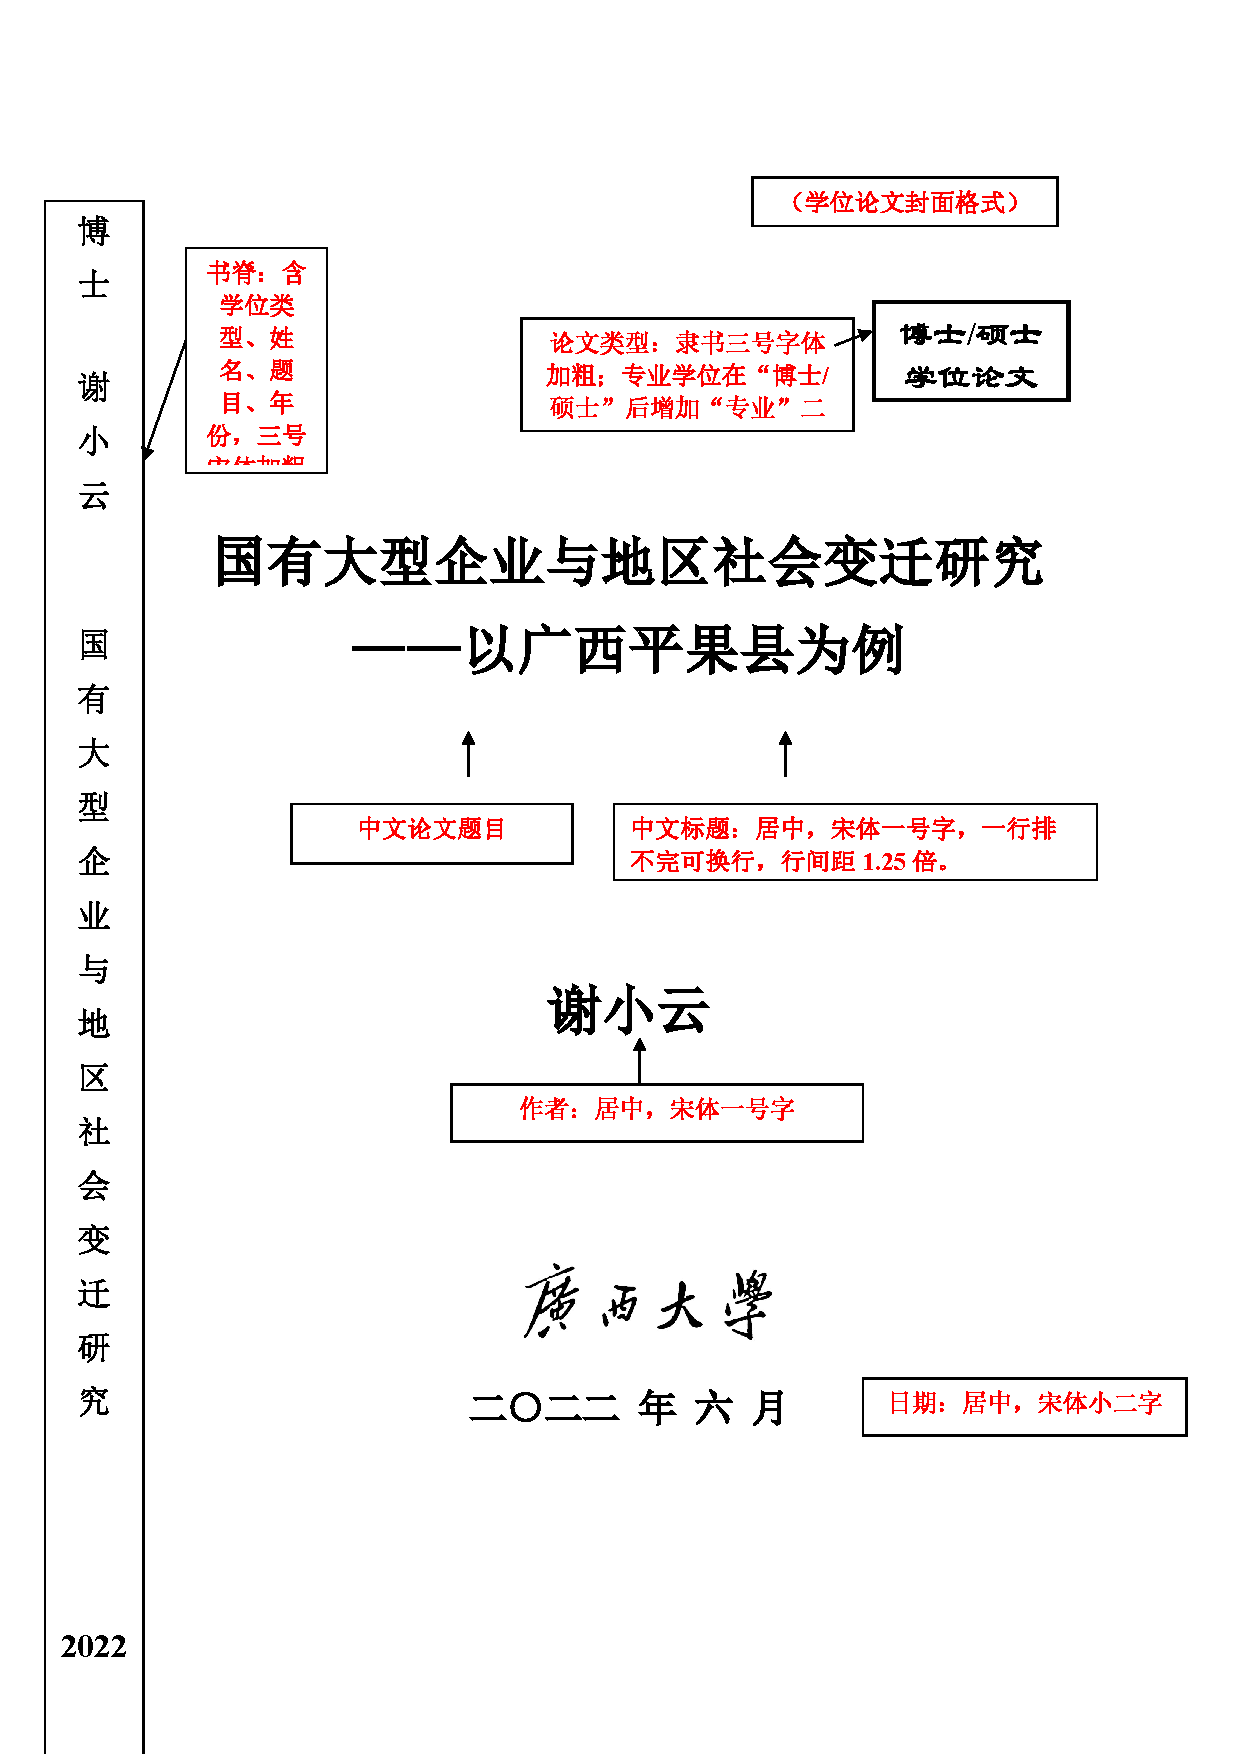
\includepdf[pages={-}]{毕业论文封面.pdf}


% 设置摘要、目录部分页码
\setcounter{page}{1} % 重置页码
\pagenumbering{Roman}
\pagestyle{fancy} % 清除原页眉页脚样式
\fancyhf{}
\fancyfoot[C]{\thepage} % 在页脚中间添加页码


%% 中文摘要
\section*{\ArticleTitle}
\begin{cnabstract}\addcontentsline{toc}{section}{摘\ 要}
\fontsize{14pt}{17.5pt}\selectfont %设置字体为四号,行间距1.25倍

% 本研究聚焦于雾天环境下交通小目标检测这一关键课题,旨在为智能交通系统和无人技术在复杂气象条件下的应用提供高效、鲁棒的解决方案。随着智能交通系统的快速发展,交通物体的检测与识别对于保障道路安全和优化交通管理具有不可替代的重要作用。然而,雾天等恶劣天气条件严重干扰了无人机拍摄图像的质量,导致基于良好天气图像训练的检测模型性能大幅下降,尤其对于小目标检测而言,挑战更为严峻。

% 雾天环境下交通小目标检测面临着多重问题与挑战。雾气的弥散作用导致图像能见度降低、对比度下降,目标轮廓模糊不清,边界难以辨认,这使得基于良好天气图像训练的检测模型难以适应,准确识别目标的能力受到极大限制。小目标在图像中所占像素比例极低,传统检测算法受限于分辨率和信息丢失问题,难以有效捕捉和识别这些小目标。在雾天条件下,小目标检测的难度被进一步放大,去雾过程可能导致目标细节的丢失,影响检测精度;不同去雾算法在不同雾天场景下的适用性和稳定性存在差异;去雾与检测算法的融合优化尚未达到理想状态,两者的协同作用未能充分发挥,导致整体检测系统的性能提升有限。

% 为应对上述挑战,本研究提出了一系列创新性的方法。在目标检测方面,以 YOLOv11 算法为基础,提出了改进的 EX-YOLO 算法。通过深入分析 YOLOv11 网络结构,发现其在交通小目标检测中存在浅层特征图分辨率不足、跨尺度特征融合效率低等问题。为此,引入了改进的特征融合模块 SPPC,融合 SPPF 模块的多尺度特征提取能力和 CAM 的特征增强能力,显著提升了对小目标的特征捕获能力。同时,采用轻量化的卷积模块 DBSS 替代原始模块,降低了计算复杂度,使其更适用于资源受限设备。此外,引入 NWD 损失函数与 DIoU 损失函数相结合,提高了对小目标定位的精准度。在图像去雾方面,基于 CycleGAN 网络提出了改进的 CGANFormer 算法。将 Transformer 模块与 CycleGAN 的生成器网络相结合,利用其自注意力机制捕捉图像全局依赖关系,突破了传统卷积局部感受野的限制,能够更精准地还原雾天图像中的细节信息,如物体边缘和纹理。同时,采用局部 - 全局结合的判别器架构,局部判别器关注图像细节特征,全局判别器把控图像宏观特征,提升了去雾图像的整体质量和视觉效果。

% 本研究方法在多个数据集上进行了全面验证,取得了显著的效果。EX-YOLO 算法在保持较高检测精度的同时大幅降低了计算量,与 YOLOv11s、YOLOv10s 和 YOLOv9s 等模型相比,在 mAP、P、R 等关键指标上均展现出优异的综合性能,尤其在小目标检测任务中具有很强的竞争力,有效平衡了精度与效率,满足了无人机等有限设备环境下的实际应用需求。CGANFormer算法与AOD-Net、FFA-Net、CGA-Net等网络模型对比,表现出更有效的去雾性能。CGANFormer 与 EX-YOLO 算法的结合在雾天图像去雾和目标检测联合实验中表现出色,在 FOG-TT100K 和 FOG-VisDrone 数据集上的精确度、召回率和 mAP 等指标上均取得显著提升,证明了该算法在无人机等资源受限设备上进行实时目标检测的可行性,有效解决了雾天环境下交通目标检测的难点问题。

% 本研究在雾天环境下交通小目标检测领域具有重要的意义。一方面,通过改进图像去雾和目标检测算法,为智能交通系统在恶劣天气条件下的稳定运行提供了技术保障,有助于提高道路安全和交通管理效率。另一方面,研究成果推动了计算机视觉技术在无人领域的应用,为无人机在复杂环境中的交通监测、目标识别等任务提供了更可靠的解决方案,促进了无人技术的进一步发展。此外,本研究提出的算法在保持高性能的同时降低了计算资源需求,有利于降低智能交通系统和无人设备的硬件成本,提高其实用性和可推广性。未来,随着相关技术的不断完善和优化,本研究成果有望在更广泛的交通场景和气象条件下发挥更大的作用,为构建更加智能、安全、高效的交通体系奠定坚实的基础。

本研究聚焦于雾天环境下交通小目标检测的前沿课题,致力于攻克低能见度条件下无人机拍摄图像中小目标识别的难题,为智能交通系统与无人技术的深度发展提供关键技术支持。雾天图像受大气散射模型影响,呈现出对比度降低、颜色失真及目标轮廓模糊等特征,致使传统检测算法性能显著退化,尤其对小目标的检测精度与召回率难以满足实际应用场景需求。在复杂交通场景中,小目标如行人、非机动车以及远处交通标志等,因所占像素比例极低且易受背景干扰,检测难度急剧攀升。

针对上述挑战,本文提出基于改进 YOLOv11 网络的交通小目标检测算法 EX-YOLO 与基于改进 CycleGAN 网络的去雾还原算法 CGANFormer,并将二者有机融合,构建出适配雾天场景的高效目标检测系统。在目标检测环节,EX-YOLO 算法引入多尺度特征融合模块 SPPC,融合 SPPF 模块的池化操作与 CAM 模块的多尺度卷积,有效增强小目标特征提取能力;搭载轻量化卷积模块 DBSS,以深度可分离卷积及 SimAM 注意力机制替代原始标准卷积,大幅削减计算量;采用 DIoU 损失与 NWD 损失函数相结合的优化策略,精准定位小目标。在图像去雾环节,CGANFormer 算法革新传统 CycleGAN 架构,将 Transformer 模块嵌入生成器网络,利用自注意力机制捕捉全局依赖关系,突破卷积局部感受野限制;判别器引入局部 - 全局结合架构,协同保障去雾图像细节与整体质量。

实验验证表明,EX-YOLO 算法相较于 YOLOv11s,在 TT100K 数据集上 mAP0.5 提升至 0.893,计算量降低至 17.0 GFLOPs;在 VisDrone 数据集上 mAP0.5 达 0.390,计算量仅 15.4 GFLOPs,较基准模型均有显著优化。CGANFormer 算法在 NYU2 数据集 PSNR 达 21.0121、SSIM 为 0.9426,在 Dense-Haze 数据集 PSNR 为 16.8625、SSIM 为 0.5879,去雾效果全面超越对比算法。二者融合后的系统在 FOG-TT100K 数据集上 mAP0.5 达 0.592,精确度与召回率分别提升至 0.699 和 0.449;在 FOG-VisDrone 数据集上 mAP0.5 为 0.397,精确度与召回率分别为 0.721 和 0.074,综合性能指标显著占优。

本研究的成果为雾天交通小目标检测开辟了新的路径,不仅有效提升了复杂气象条件下智能交通系统的感知能力,还为无人机在低能见度环境下的广泛应用奠定了坚实基础,推动了计算机视觉技术在实际交通管理与无人驾驶领域的深化落地,具有重大的现实意义与应用前景。
\\
\\
\heiti 关键词:
\songti 深度学习\ \ 雾天目标检测\ \ 改进YOLO算法\ \ 循环对抗生成网络\ \ Transformer模块

\end{cnabstract}
\pagebreak


%% 英文摘要
\section*{\ArticleTitleEn}
\begin{enabstract}\addcontentsline{toc}{section}{ABSTRACT}
\fontsize{14pt}{17.5pt}\selectfont %设置字体为四号,行间距1.25倍

% This research focuses on the key topic of detecting small traffic targets in foggy environments, aiming to provide efficient and robust solutions for the application of intelligent transportation systems and unmanned technologies under complex meteorological conditions. With the rapid development of intelligent transportation systems, the detection and identification of traffic objects plays an irreplaceable and important role in ensuring road safety and optimizing traffic management. However, bad weather conditions such as foggy days have seriously interfered with the quality of the images taken by drones, resulting in a significant decline in the performance of detection models based on good weather image training, especially for small target detection, which is more serious.

% Traffic small target detection faces multiple problems and challenges in a foggy environment. The diffusion effect of fog leads to reduced image visibility, reduced contrast, blurred target contours, and unrecognizable boundaries, which makes it difficult for detection models based on good weather image training to adapt, and the ability to accurately identify targets is greatly limited. The pixel ratio of small targets in the image is extremely low. Traditional detection algorithms are limited by resolution and information loss problems, and it is difficult to effectively capture and identify these small targets. Under the condition of foggy weather, the difficulty of small target detection is further amplified. The defogging process may lead to the loss of target details, affecting the detection accuracy. There are differences in the applicability and stability of different fogging algorithms in different foggy weather scenarios. The integration optimization of fogging and detection algorithms has not reached the ideal state, and the synergy of the two Failure to give full play has led to a limited improvement in the performance of the overall detection system.

% In order to meet the above challenges, this study puts forward a series of innovative methods. In terms of target detection, an improved EX-YOLO algorithm is proposed based on the YOLOv11 algorithm. Through in-depth analysis of the YOLOv11 network structure, it is found that it has problems such as insufficient resolution of shallow feature map and low cross-scale feature fusion efficiency in traffic small target detection. To this end, an improved feature fusion module SPPC has been introduced to integrate the multi-scale feature extraction ability of the SPPF module and the feature enhancement ability of CAM, which significantly improves the feature capture ability for small targets. At the same time, the use of lightweight convolutional module DBSS to replace the original module reduces the complexity of computing and makes it more suitable for resource-limited devices. In addition, the combination of the NWD loss function and the DIoU loss function has improved the accuracy of small target positioning. In terms of image defogging, an improved CGANFormer algorithm is proposed based on the CycleGAN network. Combining the Transformer module with CycleGAN's generator network, it uses its self-attention mechanism to capture the global dependency of images, breaks through the limitations of traditional convolutional local sensing fields, and can more accurately restore detailed information in the foggy images, such as object edges and textures. At the same time, the local-ground combined discister architecture is adopted. The local discisiser focuses on the detailed characteristics of the image, and the global discisifier controls the macro characteristics of the image, which improves the overall quality and visual effect of the defogging image.

% This research method has been comprehensively verified on multiple data sets and achieved remarkable results. The EX-YOLO algorithm greatly reduces the calculation amount while maintaining high detection accuracy. Compared with benchmark models such as YOLOv11s, YOLOv10s and YOLOv9s, it shows excellent comprehensive performance in key indicators such as mAP, P and R, especially in It has strong competitiveness in small target detection tasks, effectively balances accuracy and efficiency, and meets the actual application needs of limited equipment environments such as unmanned aerial vehicles. The combination of CGANFormer and EX-YOLO algorithm performed well in the joint experiments of foggy image defogging and target detection, and the accuracy, recall rate and mAP on the FOG-TT100K and FOG-VisDrone data sets are all taken. It has been significantly improved, and at the same time, the computing volume has been significantly reduced, showing a low computational complexity, which proves the feasibility of the algorithm for real-time target detection on resource-limited equipment such as drones, and effectively solves the difficult problem of traffic target detection in a foggy environment.

% This research is of great significance in the field of traffic small target detection in a foggy environment. On the one hand, by improving image defogging and target detection algorithms, it provides technical guarantee for the stable operation of intelligent traffic systems under bad weather conditions, which is conducive to improving road safety and traffic management efficiency. On the other hand, the research results have promoted the application of computer vision technology in the unmanned field, provided more reliable solutions for traffic monitoring, target identification and other tasks of drones in complex environments, and promoted the further development of unmanned technology. In addition, the algorithm proposed in this study reduces the demand for computing resources while maintaining high performance, which is conducive to reducing the hardware cost of intelligent transportation systems and unmanned equipment, and improving practicality and generalization. In the future, with the continuous improvement and optimization of relevant technologies, the results of this research are expected to play a greater role in a wider range of traffic scenarios and meteorological conditions, and lay a solid foundation for building a more intelligent, safe and efficient transportation system.

This research focuses on the cutting-edge topic of traffic small target detection in a foggy environment. It is committed to overcoming the problem of identifying small and small targets in drone images under low visibility conditions, and providing key technical support for the in-depth development of intelligent transportation systems and unmanned technology. Affected by the atmospheric scattering model, the foggy images show characteristics such as reduced contrast, color distortion and blurred target contours, resulting in a significant degradation of the performance of traditional detection algorithms. In particular, the detection accuracy and recall rate of small targets are difficult to meet the requirements of practical application scenarios. In complex traffic scenarios, small targets such as pedestrians, non-motorized vehicles and distant traffic signs, etc., are extremely low in pixel ratio and susceptible to background interference, and the difficulty of detection increases sharply.

In response to the above challenges, this paper proposes the traffic small target detection algorithm EX-YOLO based on the improvement of the YOLOv11 network and the defogging reduction algorithm CGANFormer based on the improvement of the CycleGAN network, and organically integrates the two to build an efficient target detection system adapted to the foggy scene. In the target detection link, the EX-YOLO algorithm introduces the multi-scale feature fusion module SPPC, integrates the pooled operation of the SPPF module and the multi-scale convolution of the CAM module, and effectively enhances the ability to extract small target features; equipped with a lightweight convolution module DBSS, it replaces the original standard convolution with deep separable convolution and SimAM attention mechanism, and greatly reduces the calculation volume; adopts the optimization strategy of combining DIoU loss and NWD loss function to accurately locate small targets. In the image defogging link, the CGANFormer algorithm innovates the traditional CycleGAN architecture, embeds the Transformer module into the generator network, uses the self-attention mechanism to capture global dependencies, and breaks through the convolutional local sensing field restrictions; the discriminator introduces a local-pheral combination architecture to jointly ensure the details and overall quality of the defogging image.

Experimental verification shows that compared with YOLOv11s, the EX-YOLO algorithm increased mAP0.5 to 0.893 on the TT100K data set, and the calculation volume was reduced to 17.0 GFLOPs; the mAP0.5 reached 0.390 on the VisDrone data set, and the calculation volume was only 15.4 GFLOPs, which was significantly optimized compared with the benchmark model. The CGANFormer algorithm has a PSNR of 21.0121 and SSIM of 0.9426 in the NYU2 data set. In the Dense-Haze data set, PSNR is 16.8625 and SSIM is 0.5879. The defogging effect comprehensively surpasses the comparison algorithm. After the integration of the two, the system has mAP0.5 up to 0.592 on the FOG-TT100K data set, and the accuracy and recall rate are increased to 0.699 and 0.449 respectively; mAP0.5 is 0.397 on the FOG-VisDrone data set, and the accuracy and recall rate are 0.721 and 0.074 respectively, and the comprehensive performance indicators are significantly superior.

The results of this research have opened up a new path for the detection of small targets in foggy traffic, which not only effectively improves the perception ability of intelligent traffic systems under complex meteorological conditions, but also lays a solid foundation for the wide application of drones in low-visibility environments, and promotes the deepening implementation of computer vision technology in the field of actual traffic management and unmanned vehicles, which is of great practical significance and application prospects.
\\
\\
\textbf{KEW WORDS:} Deep learning;  Target detection on foggy days;  Improve the YOLO algorithm;  CycleGAN Net;  Transformer Block
\end{enabstract}
\pagebreak

%% ------------------------------ %%
{\hypersetup{linkcolor=black}\tableofcontents}
\newpage
\setcounter{page}{1} % 重置页码
\pagenumbering{arabic} % 开始阿拉伯数字编码
% R:页面右边; L:页面左边; C:页面中间
\pagestyle{fancy}%清除原页眉页脚样式
\fancyhf{}
% \fancyhead[L]{\lishu \fontsize{12pt}{15pt}\selectfont 广西大学硕士学位论文}
\fancyhead[L]{\fontsize{12pt}{15pt}\selectfont 广西大学硕士学位论文} %\leftmark:表示“一级标题”
% \fancyhead[C]{\rightmark} %\rightmark:表示“二级标题”
\fancyhead[R]{\fontsize{12pt}{15pt}\selectfont \ArticleTitle}%\thepage:表示“页码”
\fancyfoot[C]{\thepage} % 在页脚中间添加页码
%% ------------------------------ %%


\section{绪论\label{绪论}}

\subsection{课题背景及研究的目的和意义}

随着智能交通系统和无人技术的迅猛发展,交通物体的检测和识别已成为确保道路安全和优化交通管理的关键环节。大量研究表明,这一技术对于构建高效、安全的现代交通体系具有不可替代的重要作用 \cite{review1, review2, review3}。近年来,无人机图像目标检测技术取得长足进步,一系列创新方法不断涌现\cite{ye2022dense, Mffsodnet, sun2022rsod},这些成果为无人机图像目标检测领域带来了显著的性能提升,使其在良好天气和充足光照条件下的检测效果达到令人满意的水平,为实际应用奠定了坚实基础。

然而,实际的交通环境远比理想条件复杂多变,特别是在劣天气环境下,无人机拍摄图像的质量会受到严重干扰和影响。其中,雾天环境对图像质量的破坏尤为突出,雾气的弥散作用导致图像能见度大幅降低、对比度显著下降,目标轮廓变得模糊不清,边界难以辨认。这种情况下,基于良好天气图像训练出的检测模型往往难以适应,准确识别目标的能力受到极大限制,检测性能出现明显下滑,无法满足实际应用中对高精度检测的需求。

小目标检测在无人机交通物体检测场景中同样面临诸多严峻挑战。对于交通物体检测而言,小目标如远处的行人、交通标志等,由于其体积小、在复杂背景中易被遮挡,在图像中所占像素比例极低。传统检测算法受限于分辨率和信息丢失问题,难以有效捕捉和识别这些小目标,检测效果不尽如人意,进而影响整个智能交通系统的可靠性和稳定性。尤其在夜间和恶劣天气等复杂交通环境下,对检测算法的鲁棒性提出了更高的要求。此时,准确识别行人和其他交通参与者变得尤为重要,这不仅关乎智能交通系统的安全运行,更是无人驾驶技术得以进一步发展的关键前提,任何微小的检测失误都可能引发严重的后果。

在雾天环境下,小目标检测的难度被进一步放大。雾天图像质量的退化使得原本就难以识别的小目标更加模糊不清,目标的特征信息被大量遮蔽和混淆,特征提取过程变得更加困难重重。尽管一些研究开始关注这一棘手问题,并尝试提出相应的改进方法,例如通过结合图像去雾技术和目标检测算法,先对雾天图像进行预处理,增强图像质量,改善能见度和对比度,再进行目标检测,从而在一定程度上提高了检测性能。但目前这些方法仍存在诸多亟待解决的挑战,如去雾过程可能导致目标细节的丢失,影响检测精度;不同去雾算法在不同雾天场景下的适用性和稳定性存在差异;去雾与检测算法的融合优化尚未达到理想状态,两者的协同作用未能充分发挥,导致整体检测系统的性能提升有限。

雾天环境和小目标特性的复杂组合给无人机图像目标检测带来了前所未有的难题。如何有效整合图像去雾、图像增强技术与先进的深度学习检测算法,形成一套高效、鲁棒的检测系统,以提高在雾天环境下对小目标的检测能力,已成为当前计算机视觉和交通流量管理领域亟待攻克的重要研究课题。解决这一难题对于提升无人机在实际复杂环境中的应用效果、推动智能交通系统和无人驾驶技术的发展具有极其重要的理论意义和应用价值,有望为未来智能交通体系的构建提供坚实的保障。


\subsection{国内外研究现状}

\subsubsection{目标检测算法}

目标检测作为计算机视觉领域的核心任务之一,在众多实际应用场景中发挥着关键作用,如自动驾驶、智能安防、医疗影像分析、机器人视觉等。它的目标是在图像或视频中准确识别出特定目标物体的位置和类别。随着计算机技术的飞速发展,目标检测技术经历了从简单到复杂、从低效到高效的演变过程,其理论和方法不断推陈出新,以满足日益增长的实际应用需求。

早期目标检测依赖人工设计的传统特征,如 Haar \cite{Haar_like} 特征,其能捕捉图像边缘等信息,通过积分图快速计算特征值,基于此的 Viola - Jones 人脸检测算法借助 AdaBoost 算法选择训练特征构建级联分类器实现高效面部检测。还有基于边缘、纹理特征等的方法,这类传统特征提取方式虽直观、计算复杂度低,但对复杂场景适应性差,难以自动学习深层规律,对目标各种变化敏感致检测精度受限。
后机器学习发展,浅层学习方法如利用 SVM 分类的目标检测受关注\cite{svm},通常先用 SIFT、HOG 等特征提取手段获取目标特征再用分类器区分目标与背景。其中 HOG 特征描述子在行人检测等任务表现好,但浅层学习方法在特征提取阶段仍有限,特征表达能力不足,难全面刻画复杂目标特征,且训练需大量标注数据,面对新类别、场景泛化能力弱。

深度学习的兴起为目标检测带来了革命性的变化。深度卷积神经网络(CNN)\cite{cnn}能够自动学习图像中的深层特征表示,从而极大地提高了目标检测的性能。
早期的基于深度学习的目标检测方法之一是 R-CNN\cite{fast_rcnn,mask_rcnn}。它首先通过选择性搜索等区域提议方法生成候选区域,然后对每个候选区域进行特征提取和分类。然而,R-CNN 存在计算速度慢、训练过程复杂等缺点,因为它对每个候选区域都要进行独立的 CNN 计算。

为了克服这些问题,Fast R-CNN 相继提出。Fast R-CNN 将整个图像输入网络一次性提取特征,然后对所有候选区域共享这些特征,大大提高了计算效率。之后,Faster R-CNN 进一步引入了区域提议网络(RPN)来替代传统的区域提议方法,实现了端到端的训练,进一步提升了检测速度和精度,成为目标检测领域的一个重要里程碑。

随后,YOLO(You Only Look Once)\cite{yolov1, yolov2, yolov3, yolov4, yolov6, yolov7, yolov9, yolov10, yolov11}系列算法和 SSD(Single Shot Multibox Detector)\cite{ssd, dssd}等单阶段目标检测算法崭露头角。YOLO 将目标检测任务视为一个回归问题,将图像划分为多个网格,每个网格同时预测多个边界框和类别概率,实现了快速、实时的目标检测,在一些对速度要求较高的应用场景中表现出色。

YOLOv1 以提升检测速度为核心,将检测任务视为回归问题求解,不过在准确性方面尚有不足。YOLOv4 在此基础上引入 Mish 激活函数、CSPDarknet 主干网络\cite{csp}及 SPP 模块等先进组件,显著提升检测精度与速度。YOLOv9 首次引入混合 CNN - Transformer 主干网络架构,并融合可编程梯度信息(PGI)与广义高效层聚合网络(GELAN),使小目标检测性能实现质的飞跃。YOLOv10 创新性地引入无 NMS训练机制与多尺度特征融合技术,进一步优化小目标检测性能。YOLOv11 则通过引入 C3k2 和 C2PSA 模块,对网络结构与训练策略进行深度优化,再次提升检测精度与速度。这些持续迭代的改进,不仅全方位提升模型检测精度与速度,还显著增强其在复杂场景下的稳健性与适应性,为无人机小目标检测等前沿应用提供坚实可靠的技术支撑。

然而,尽管 YOLO 的单级结构在效率上独树一帜,小目标检测仍面临诸多挑战。小目标像素稀缺,极易受背景干扰,致使检测准确性下降。FPN\cite{fpn}应运而生,其借助自上而下的功能融合机制,有效提升多尺度检测能力。

在损失函数优化领域,传统 YOLO 采用的二进制交叉熵(BCE)与均方误差(MSE)\cite{mse}对小目标检测中边界细微变化敏感度较低,易引发准确性降低。IoU 损失函数系列,包括 GIoU\cite{giou}、DIoU 与 CIoU\cite{diou},通过对预测框与真实框重叠区域优化,显著提高检测精度。
Yang 等人\cite{gwd}提出的 GWD(Generalized Wasserstein Distance)损失函数,创新性地通过位置关系测量边界框,提升定向物体检测准确性,但对小目标的敏感度仍有待提高。

为攻克小目标检测难题,研究人员致力于优化 FPN 结构。
特征金字塔网络(FPN)开创性地整合不同尺度特征,增强对各类目标的检测能力。
FPN 由 Tsung - Yi Lin 等人于 2017 年首次提出,通过自上而下路径在特征图上取样,巧妙融合高级语义信息与低级空间信息,使其在小目标检测领域表现卓越。PANet(Path Aggregation Network)\cite{pan}与 BiFPN(Bidirectional Feature Pyramid Network)\cite{bifpn}等网络在 FPN 基础上推陈出新。
PANet 增加自下而上的路径聚合与全景特征融合,助力浅层信息向深层高效传输,适用于复杂背景下的小目标检测。
BiFPN 则借助双向特征融合与权重学习机制,自适应调整特征层贡献,进一步优化多尺度检测效果。
Su Peng 等人\cite{mod-yolo}设计的 GRF - SPPF 模块,通过整合全球与本地传感现场信息,有效降低不同尺度对检测的影响。
Li Haibin 等人\cite{yolo-pl}提出的 E - PAN(Enhanced Path Aggregation Network),通过相同尺度近似采样与残差操作,强化多尺度特征融合,过滤复杂背景信息以提升检测精度。
Zhao Chao 等人\cite{rdd-yolo}设计的双特征金字塔网络(DFPN),增强特征融合能力,提高整体检测性能。
Zhang Yan 等人\cite{dsp-yolo}打造的轻量级且对细节敏感的 DsPAN,强化本地特征与细节,减少特征融合过程中的信息损失。
然而,深度学习算法在追求高精度过程中,通常伴随着计算开销的显著增加,在有限计算资源约束下,实现实时检测面临巨大挑战。


\subsubsection{图像去雾还原算法}

图像去雾是计算机视觉关键技术之一,在安防监控、自动驾驶等众多实际应用场景中,大气散射常导致图像退化,出现对比度降低、颜色失真、细节模糊等问题,影响后续图像分析与识别任务准确性,深入研究图像去雾还原算法技术理论发展及现状意义重大。

20 世纪 80 年代,大气光学相关研究为图像去雾奠定基础,大气散射模型被提出,阐述光线传播受散射和吸收作用机制,因当时假设大气是均匀介质且对不同波长光线散射作用相同,模型较简单,后续研究引入非均匀大气介质假设,考虑不同波长光线散射特性差异,使模型更贴近实际。模型可表示为:
\begin{equation}
    \label{eq:haze}
    I(x) = J(x)t(x)+A(1-t(x))
\end{equation}

公式 \ref{eq:haze} 中,$I(x)$ 表示观测到的含雾图像,$J(x)$ 是无雾场景的清晰图像,$t(x)$ 为大气透射率,反映了场景中光线传播时未被散射和吸收的比例,$A$ 是大气光照,在远处场景点,大部分光线被散射,此时观测到的像素值趋近于大气光照。

20 世纪末至 21 世纪初,随着计算机视觉技术发展,研究者利用图像先验知识去雾,物理模型去雾方法优势凸显,其中基于暗通道先验方法地位重要,其通过计算暗通道图、估算透射率并与大气散射模型结合去雾。如 Dark-ControlNet \cite{Dark_ControlNet}融合冻结骨干网络与暗通道先验特征提升去雾效果,He 等人\cite{he2010single}提出的方法结合暗通道先验与雾霾成像模型恢复无雾图像,Peng 等人\cite{peng2018generalization}引入自适应色彩校正机制应对图像退化问题。

基于颜色衰减先验的方法为物理模型去雾提供了另一条有效途径,其关键在于利用雾气影响下图像亮度与饱和度之间的内在关系来实现去雾。Zhu 等人 \cite{zhu2015fast} 提出的基于颜色衰减先验的单图像去雾方法,通过构建线性模型精准估计场景深度,并借助监督学习优化参数,从而高效恢复出透射率和场景光芒,实现雾霾的有效去除。Liang 等人 \cite{liang2021single} 设计的基于衰减图引导的色彩校正方法以及细节保留的去雾方法,在色彩校正和细节保留方面表现出色。Qiu 等人 \cite{qiu2024perception} 对物理模型进行改进,创新性地结合超像素场景先验(SPSP)和简单线性迭代聚类(SLIC)等前沿技术,对去雾过程进行了深度优化。

随着人工智能技术的飞速发展,深度学习在图像去雾领域逐渐崭露头角,成为当下图像去雾的主流方向。众多基于深度学习的去雾方法不断涌现并得到广泛验证,其中包括基于生成对抗网络(GAN)、循环神经网络(RNN)以及 Transformer 架构的图像去雾方法。Dong 等人 \cite{dong2020fd} 提出的带有融合判别器的端到端生成对抗网络,用于单张图像去雾,其巧妙地以频率信息作为先验知识,有效解决了传统去雾方法中因中间参数估计不准确而引发的伪影和颜色失真问题。Ashwini 等人 \cite{ashwini2024epq} 采用差分进化算法,并创新性地结合感知损失、质量评估损失和对抗性损失对对抗生成网络进行训练,进一步提升了去雾效果。Zheng 等人 \cite{zheng2022dehaze} 提出的增强型注意力引导生成对抗网络,专门针对遥感图像去雾难题,取得了显著成效。Frants 等人 \cite{frants2023qcnn} 提出的基于鲁棒性四元数神经网络架构的单图像去雾方法,为去雾技术提供了新的思路。Guo 等人 \cite{guo2022image} 通过引入特征调制和传输感知 3D 位置嵌入模块,成功解决了 CNN 和 Transformer 之间存在的特征不一致问题。Song 等人 \cite{song2023vision} 对 Swin Transformer 的归一化层(如用 RescaleNorm 替代 LayerNorm)、激活函数(ReLU 优于 GELU)和空间信息聚合方案进行了全面改进,进一步提升了深度学习去雾方法的性能。

\subsubsection{雾天目标检测技术}

在复杂环境下的目标检测领域,雾天场景下的目标识别占据着举足轻重的地位。传统雾天目标检测技术的流程通常是,先借助图像恢复技术,像去雾算法这类手段,对雾天图像开展预处理操作,以此来提高图像的视觉质量。紧接着,将经过去雾处理的图像输入至预先训练好的目标检测模型之中进行识别工作。例如,部分研究通过引入图像增强技术,包括对比度调整或者基于物理模型的散射估计方法等,来提升雾天图像的可见性。与此同时,还有一些研究着重于设计具备鲁棒性的目标检测算法,以便能够适应去雾之后图像的特征变化情况。这种分阶段处理的模式,虽能在一定程度上减轻雾天环境对于目标检测性能产生的负面干扰,然而其存在的局限性不容忽视,即图像恢复与目标检测任务之间缺乏协同优化机制。去雾算法一般是独立于检测任务来进行优化的,这就造成生成的去雾图像可能无法充分契合目标检测对于特征表达的特有需求,进而在很大程度上限制了整体性能的进一步提升。

基于此现状,近年来研究的重点方向逐渐向联合优化去雾与目标检测这一领域倾斜\cite{liu2024oriented, liu2024approach, zhang2020unified},也就是所谓的检测友好的去雾方法。此类方法不再仅仅执着于实现高质量的图像恢复,转而致力于优化去雾过程,使其能够与检测任务的特征学习相互适配。

在诸如雾天、雨天这类降级环境下,目标特征往往会被掩盖或者模糊化,倘若直接在降质图像上开展目标识别,其效果通常都不尽如人意\cite{freire2024beyond}。不过,图像恢复技术,像去雾、去噪等操作,能够有效改善图像质量,进而增强目标识别的性能表现。目前的研究大多将图像恢复与目标识别分割开来,主要聚焦于图像质量的评价,而鲜少有研究着重关注恢复后的图像在实际目标识别任务中所实现的性能提升情况。本研究着重探究图像恢复与目标识别之间存在的内在联系,并通过实验来验证图像恢复技术对于目标识别性能产生的实际影响。

部分研究选择直接在降质图像上开展目标识别训练工作,通过改进对比损失、利用辅助信息以及先验知识等手段来增强模型的性能。例如,Singh 等人\cite{singh2019dual}提出 DirectCapsNet 双导向胶囊网络模型,经由引入 HR-anchor 损失以及目标重建损失,借助高分辨率图像辅助训练,从而显著提升了低分辨率(VLR)图像的识别性能。Sindagi 等人\cite{sindagi2020prior}构建了一种基于先验知识的无监督领域自适应目标检测框架,通过引入先验对抗损失以及残差特征恢复块。Zhong 等人\cite{zhong2024dehazing}设计出先验知识引导网络,依托大气散射模型以及共现关系图来引导特征学习。

而另外一些研究则是先训练用于恢复图像的模型,将降质图像恢复之后再输入至模型中进行检测。这类方法普遍分为恢复与识别两个阶段,先训练图像恢复算法,随后在增强后的图像上对预训练的对象识别算法开展评估工作。由于恢复和识别任务相互分离,实验较难验证它们之间存在的相互作用情况。例如,Hu 等人\cite{hu2024beyond}提出名为 HRAOD 的雾霾稳健航空目标检测方法,引入图像去雾方法作为目标检测的预处理步骤。而少数研究将去雾模块同检测模块进行联合训练,像 Liu 等人\cite{liu2024oriented}提出遥感图像目标检测模型 DFENet,引入去雾特征增强模块以及动态平衡机制。Liu 等人\cite{liu2024approach}提出一种轻量化目标检测模型,实现与去雾模块的联合优化。Zhang 等人\cite{zhang2020unified}以雾霾密度为先验知识,经由残差感知雾霾密度分类器、密度感知去雾网络以及密度感知目标检测器开展相关工作。

与上述各类方法存在差异的是,本文同时将目光聚焦于图像的质量恢复以及恢复后图像的目标检测效果方面。通过预先训练改进后的生成器和判别器,以此确保图像质量恢复的效果得以保障,同时运用该网络来制作模拟雾天场景下的数据集。将预训练完成的生成器与改进后的目标检测进行联合优化,使得生成器所生成的去雾图像能够更加契合目标检测任务的需求,进而进一步提升了检测性能表现。


\subsection{论文研究的主要内容及组织架构}

\subsubsection{论文研究内容}

在雾霾天气条件下,由于特定天气信息的干扰,所拍摄的图像能见度较低,尤其在交通路口,目标数量众多且种类相对单一,呈现出目标物密集、尺度多样化等特性。在低能见度的雾天环境下,监测采集的图像不仅视觉效果欠佳,还存在噪声较高的问题,致使目标检测的难度显著增大。

与一般目标检测领域相比,雾天环境下交通路口的目标检测识别面临更大的挑战。行人、车辆以及交通标志的检测工作面临诸多困难,尤其是图像中远处尺寸较小的交通标志,其特征提取难度较大。为应对这一复杂情况,本文以图像去雾和不同尺寸目标检测作为研究重点,对相关算法进行了改进与优化,致力于提升雾霾天气下行人、车辆以及交通标志检测算法的效能。

针对雾天图像去噪问题,本文提出基于对抗生成网络的去雾方法,旨在生成干净清晰的图像。我们构建了基于 CycleGAN \cite{cgan}的去雾网络 CGANFormer,该网络采用全局 - 局部鉴别器结构,能够有效应对空间变化的雾霾天气状况。同时,为更好地保存细节信息,设计了融合 Transformer 模块与残差块连接的编码 - 解码生成器架构,以生成高质量的无雾图像。

区别于传统的依赖大气散射模型参数估计的方法,本文通过定义一种颜色损失,并将其与感知损失相结合,共同构成 CycleGAN 中的损失函数。这一改进措施不仅提高了纹理信息恢复的质量,还能够生成具有鲜艳颜色的图像,有效缓解了颜色失真的问题。

为了提升对不同尺寸行人、车辆以及交通标志的检测能力,并兼顾精确度与实时性,本文选择当前性能优良的 YOLOv11 算法作为改进基础,新算法名为 EX-YOLO。在 YOLOv11 的 SPPF 模块基础上,我们改进为 SPPC 模块,以学习更深刻的多重尺度目标信息,特别是中小目标的信息。考虑到实际应用中计算资源的限制,尤其是无人机等设备的运行需求,我们引入轻量化的卷积模块,确保算法在有限计算资源下能够高效运行。

此外,采用 DIoU 损失和 NWD 损失函数\cite{nwd},使得预测框和对小目标的识别能力更为精准和激进。这些改进措施在不显著增加计算成本的前提下,有效提升了算法在多尺度目标识别方面的能力。

本文将 CGANFormer 与改进后的 EX-YOLO 算法进行联合应用。在去雾网络的训练过程中,我们使用 NYU2\cite{nyu2}、Dense-Haze\cite{NTIRE_Dehazing_2019} 数据集进行训练。
同时,利用 TT100K\cite{tt100k}、VisDrone\cite{vd} 数据集和FOG-TT100K、FOG-VisDrone开展去雾目标检测网络的联合训练。通过精心设计的实验方案,我们对所提出的算法与不同目标检测算法进行对比实验,并开展消融实验,以系统地验证本文算法的有效性与优势。

综上所述,本文的研究内容紧密围绕雾霾天气下交通路口的目标检测问题,通过图像去雾与目标检测算法的改进与联合,力求为该领域的研究提供新的思路与方法,最终实现对行人、车辆以及交通标志等目标的高效、准确检测。

\subsubsection{论文章节安排}

第一章是绪论。
首先聚焦于雾天下无人机交通物体检测这一前沿领域,系统梳理了当前研究进展与现状,精准识别面临的关键问题与挑战。
在深度汲取与融合前人研究成果的基础上,创新性地提出了一套改进方案,旨在优化图像去雾检测算法,构建兼具高效性与健壮性的雾天交通物体检测技术方案。
最后,对整体研究内容与架构进行了系统概述,为后续各章节的深入探究及整个研究流程的有序推进提供了有力支撑。

第二章是相关理论基础。
首先系统性地阐述了目标检测的理论基础与算法体系,涵盖了从传统机器学习方法到基于深度学习的单阶段与双阶段目标检测算法。然后,聚焦于图像去雾还原领域,详细解读雾天成像原理,探讨基于深度学习的图像去雾算法的创新突破。
最后,对目标检测算法及图像去雾还原算法的评价指标进行了分析,为后续实验验证与算法性能比较提供了坚实的理论支撑与量化依据。

第三章是基于 YOLOv11 网络改进的交通小目标检测算法。
首先对 YOLOv11 网络结构进行了阐述,详尽分析了其各个模块所承载的作用,深入剖析了该网络在目标检测任务中的运作机制。
然后介绍了改进后的 EX-YOLO 网络结构,对其新增及优化的各个模块予以细致解读,明晰各模块如何协同作业以提升网络性能。
最后,通过严谨的实验设计,对 EX-YOLO 网络与其他现有多项主流网络的性能展开了全面且系统的对比分析,借助多维度的评估指标,直观呈现了 EX-YOLO 网络在目标检测领域的显著优势与优越性能表现,有力论证了改进方案的有效性与合理性。

第四章基于 CycleGAN 网络改进的去雾还原算法。
首先系统阐述了 CycleGAN 网络的运行原理,剖析了生成器与判别器的架构细节,全面展现了二者在对抗训练中的协同机制。然后聚焦于 Transformer 模块的运作机制,凭借其自注意力机制在捕捉长程依赖关系方面的优势,创新性地提出了将 Transformer 融入 CycleGAN 构成的改进网络 CGANFormer,详尽解读了改造后的网络架构如何重塑特征学习与图像映射能力。
最后,通过严谨的实验设计,验证了 CGANFormer 在图像去雾任务上相较于其他去雾网络的卓越性能。更进一步,本研究开创性地将 CGANFormer 与 EX-YOLO 目标检测网络有机结合,构建出一种全新的目标检测架构,使其在有雾或无雾天气条件下达成更精准高效的目标检测效果,为复杂环境下的视觉智能应用提供了全新的技术范式与性能突破路径。

第五章是结论与展望。
对本文中的研究内容及其结果做出总结归纳,然后分析雾天下无人机交通物体检测任务存在的不足与未来可以进一步研究的工作。

\subsection{本章小结}

本章深入阐述了在雾天环境下无人机交通物体检测领域的关键挑战与研究进展。首先,剖析了雾天环境对图像质量的负面影响,以及小目标检测在复杂交通场景中的特殊难点,明确了提升检测性能的迫切需求。接着,全面综述了目标检测算法的发展历程,从传统特征提取方法到基于深度学习的先进架构,重点关注了 YOLO 系列算法及其改进措施在小目标检测中的应用;同时,详细介绍了图像去雾技术的演变,包括传统物理模型和新兴的深度学习方法,探讨了去雾与目标检测融合的前沿研究方向。最后,本章概述了论文的研究内容与架构,提出通过优化图像去雾和目标检测算法,构建高效、鲁棒的雾天交通物体检测系统,为后续章节的具体算法改进与实验验证奠定了坚实的理论基础。

\newpage

\section{相关理论基础\label{相关工作}}

\subsection{目标检测的理论基础与算法}

\subsubsection{双阶段目标检测算法}

双阶段目标检测算法采用分步处理的策略,可分为区域候选生成阶段和区域分类识别阶段。在第一阶段,算法主要负责生成一系列可能包含目标物体的候选区域。这些候选区域是基于图像的局部特征和先验知识来提取的,例如在一些传统算法中利用滑动窗口结合图像金字塔的方式,或者在基于深度学习的算法中采用特定的区域生成网络(RPN,Region Proposal Network)来快速产生大量的候选区域。区域生成网络会扫描输入图像,基于图像的边缘、纹理等特征来预测可能的目标位置,生成大小不一、位置各异的候选区域提议(proposals)。这些候选区域通常具有一定的,数量例如几千个不等,它们覆盖了图像中可能存在的各种目标物体的潜在位置和尺度。

在第二阶段,将第一阶段生成的候选区域作为输入,对其进行更深入的特征提取和分类识别。此时,算法会针对每个候选区域提取更具有判别力的特征,通常是利用深度卷积神经网络对候选区域内的图像内容进行特征编码。然后,利用这些特征来判断该区域是否属于某一目标类别,并进一步对目标的位置进行精确回归调整,优化候选区域的边界框坐标,使其更准确地框定目标物体。这一阶段的处理通常涉及复杂的网络结构和大量的计算,目的是在候选区域的基础上实现高精度的目标分类和定位。

随着深度学习技术在计算机视觉领域的广泛应用,基于深度学习的特征提取方法成为双阶段目标检测算法的核心部分。深度卷积神经网络(CNN)\cite{cnn}通过多层卷积和池化操作,能够自动学习到图像的层次化特征表示。在双阶段目标检测算法中,通常采用预训练的深度 CNN 作为特征提取器,例如 VGGNet\cite{simonyan2014very}、ResNet \cite{he2016deep}等知名网络架构。这些网络经过在大规模图像数据集上的预训练,已经学习到了图像的通用特征表示,包括边缘、纹理、形状等低层特征以及更抽象的语义特征。

在区域候选生成阶段,特征提取网络会对输入图像进行初步的特征编码,为后续的候选区域生成提供特征基础。而在区域分类识别阶段,会进一步利用更深的网络结构对候选区域内的特征进行提取和压缩,以便更准确地区分不同目标类别。深度学习的特征提取方法相较于传统的手工特征(如 HOG、SIFT 等)\cite{Haar_like}具有明显的优势,能够更好地适应不同场景下目标物体的复杂变化,捕捉到更丰富的目标特征信息,从而为后续的目标分类和定位提供更有力的支持。

R-CNN \cite{girshick2014rich, fast_rcnn,faster_rcnn, mask_rcnn}是双阶段目标检测算法的开创性工作。R-CNN 网络结构如图 \ref{fig:rcnn} 所示。它首先利用选择性搜索算法在输入图像中生成约 2000 个候选区域。选择性搜索算法基于图像的分割和合并策略,根据颜色、纹理、大小等相似性将图像分割为多个区域,然后逐步合并相似区域,从而生成一系列不同尺度和形状的候选区域。接着,对每个候选区域进行归一化处理,调整其大小使其适应预定义的深度 CNN 输入尺寸。将归一化后的候选区域输入到深度 CNN 中(如 AlexNet)进行特征提取,得到每个候选区域的特征向量。最后,利用支持向量机(SVM)\cite{svm}分类器对候选区域进行分类,判断其属于哪个目标类别,并通过线性回归模型对候选区域的边界框坐标进行微调,以提高目标定位的精度。

\begin{figure}[htbp]
    \centering
    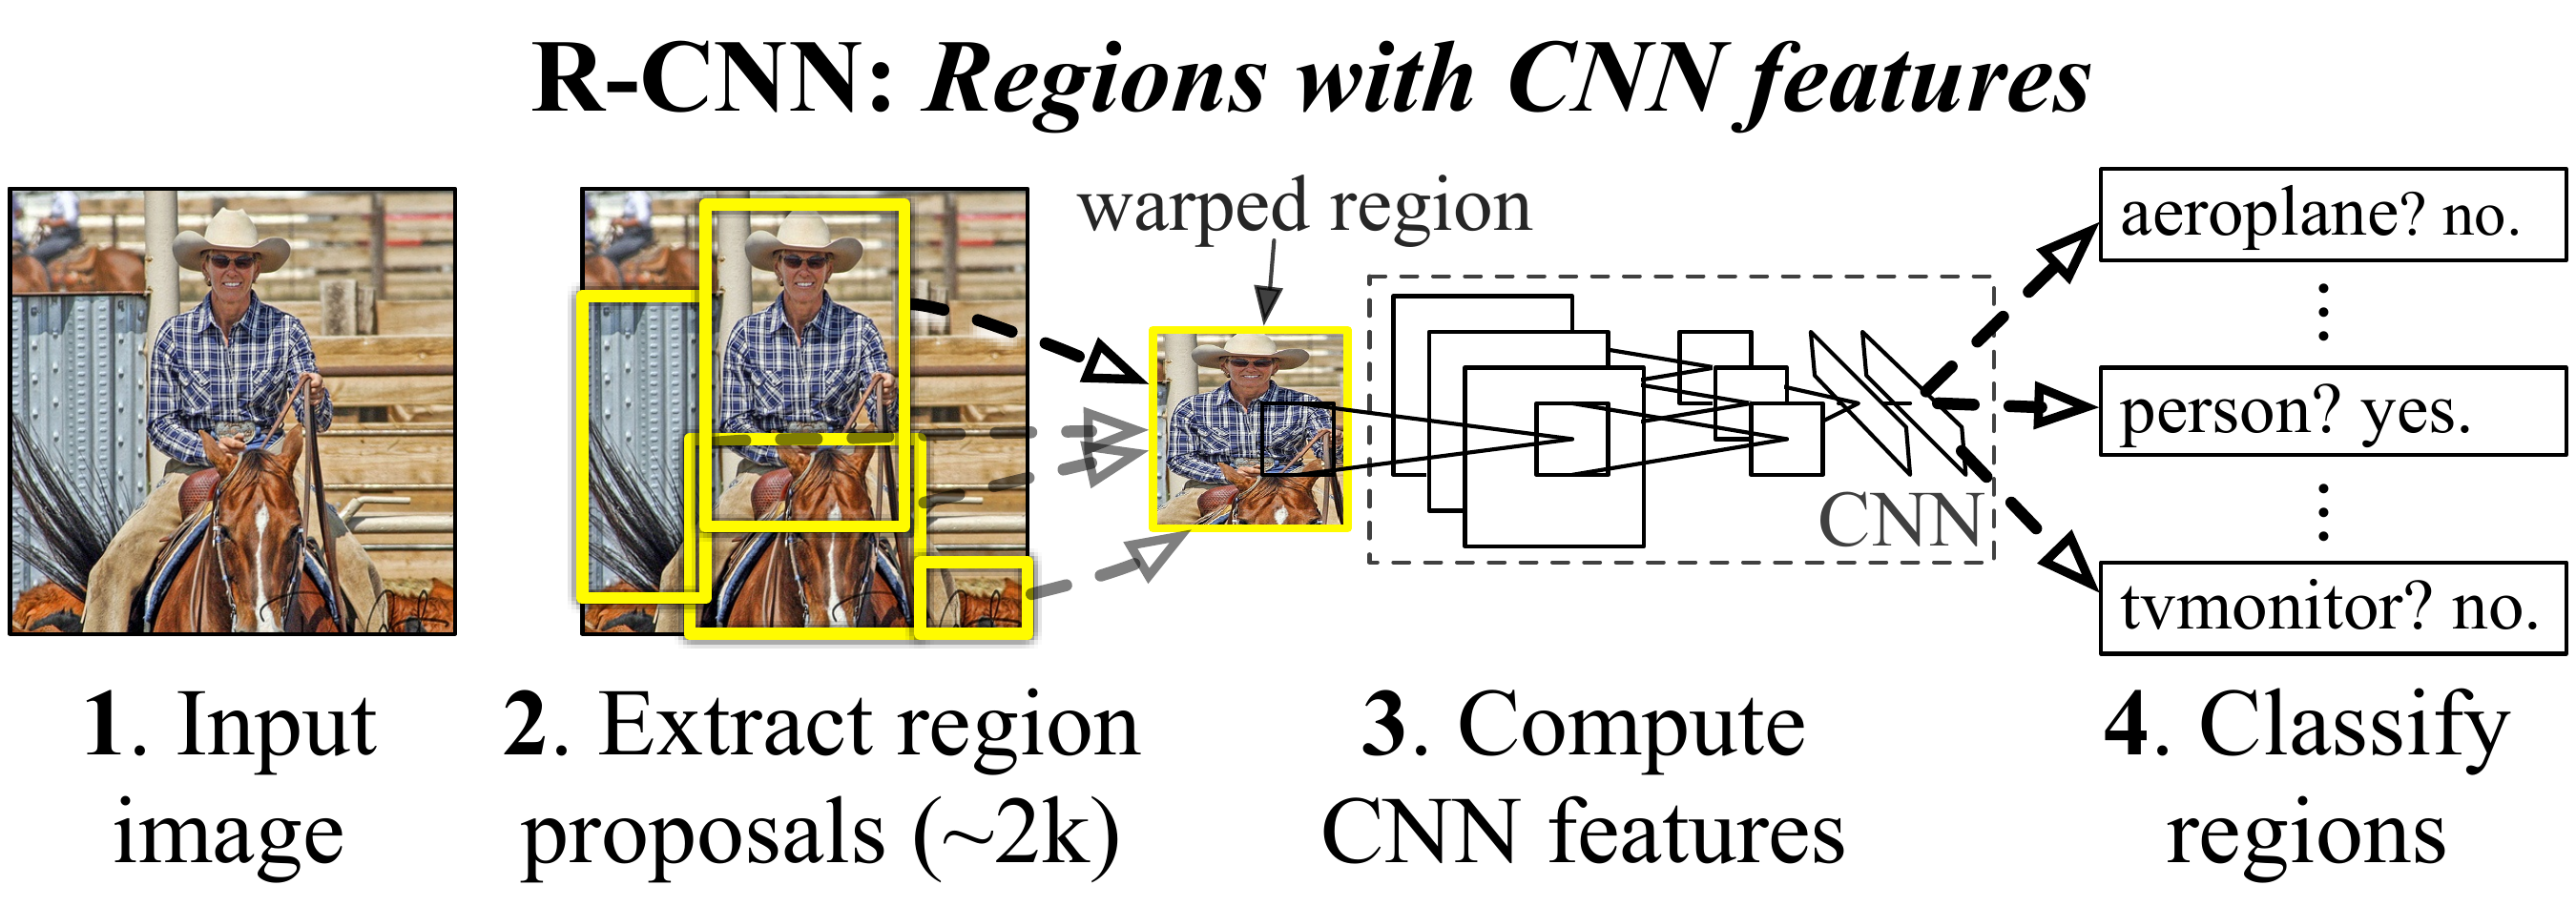
\includegraphics[width=0.7\textwidth]{../figure/rcnn.png}
    \captionsetup{font=footnotesize}
    \bicaption{RCNN 网络\cite{girshick2014rich}}{RCNN Net}
    \label{fig:rcnn}
\end{figure}

R-CNN 的提出在目标检测领域取得了重大突破,相较于传统的基于手工特征的目标检测方法,它在 PASCAL VOC 等基准数据集上取得了显著的性能提升。然而,R-CNN 也存在一些明显的不足。例如,候选区域生成过程较为耗时,选择性搜索算法的效率较低;对每个候选区域单独进行 CNN 特征提取导致计算冗余,因为大量候选区域之间存在重叠区域,重复计算了相同的图像特征,使得整个算法的处理速度较慢,难以满足实时应用的需求。

为了解决 R-CNN 中计算效率低下的问题,Fast R-CNN 对算法流程进行了改进。Fast R-CNN 网络结构如图 \ref{fig:fastrcnn} 所示。它不再对每个候选区域单独进行 CNN 特征提取,而是先将整个图像输入到深度 CNN 中进行特征提取,得到一个卷积特征图。然后,在这个卷积特征图上利用区域候选生成方法(如选择性搜索)生成候选区域,并将每个候选区域映射到卷积特征图上对应的区域。通过在卷积特征图上对候选区域进行感兴趣区域池化(ROIPooling)操作,将不同大小的候选区域池化到相同尺寸的特征向量。最后,将这些固定尺寸的特征向量输入到全连接层,进行目标分类和边界框回归。

\begin{figure}[htbp]
    \centering
    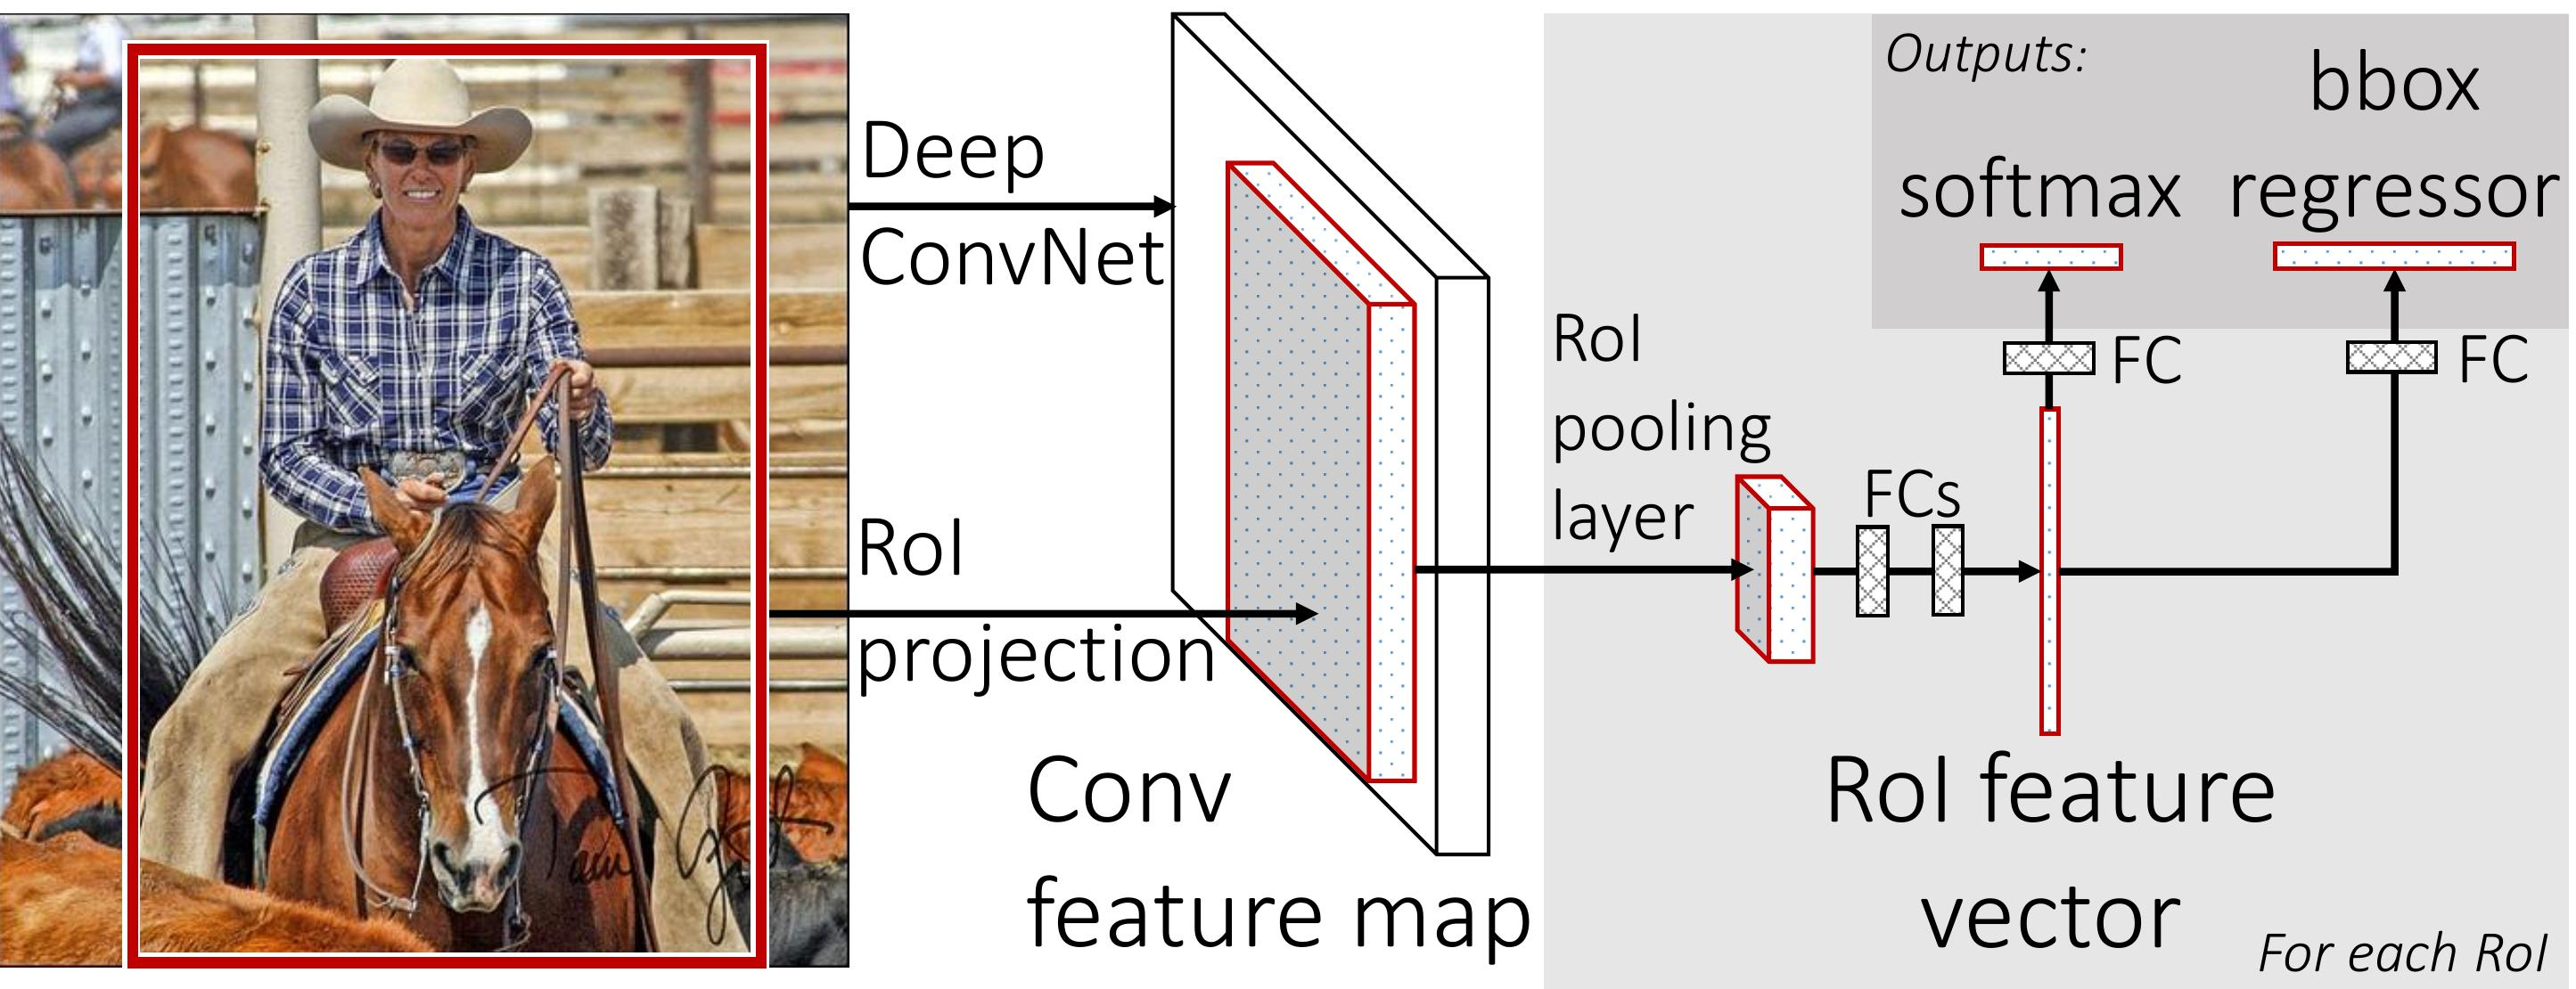
\includegraphics[width=0.7\textwidth]{../figure/fastrcnn.png}
    \captionsetup{font=footnotesize}
    \bicaption{Fast RCNN 网络\cite{fast_rcnn}}{Some descriptions of the pictures in question.}
    \label{fig:fastrcnn}
\end{figure}

这种改进方式大大提高了算法的处理速度,因为它避免了对每个候选区域重复进行卷积操作,而是在整个图像特征提取的基础上进行后续处理,有效地减少了计算量。同时,Fast R-CNN 还在训练过程中采用了多任务损失函数,将目标分类和边界框回归同时进行联合训练,进一步提升了模型的性能。然而,尽管 Fast R-CNN 在效率方面有了显著提升,但候选区域生成阶段仍然依赖选择性搜索算法,这在一定程度上限制了算法的速度和实时性。

Faster R-CNN 是在 Fast R-CNN 的基础上进一步引入了区域候选网络(RPN),实现了候选区域的自动生成,从而彻底摒弃了传统的目标区域候选生成方法。 Faster R-CNN 网络结构如图 \ref{fig:fasterrcnn} 所示。RPN 是一个全卷积网络,直接以卷积特征图为输入,通过在特征图上滑动窗口的方式,在每个位置同时预测候选区域的位置坐标和该区域属于目标物体前景或背景的概率分数。RPN 生成的候选区域经过非极大值抑制(NMS)处理后,筛选出最有可能包含目标的候选区域,并将这些区域通过 ROIPooling 层映射到固定尺寸的特征图,然后依次输入到全连接层进行目标分类和边界框回归,与 Fast R-CNN 的后续处理流程类似。

\begin{figure}[htbp]
    \centering
    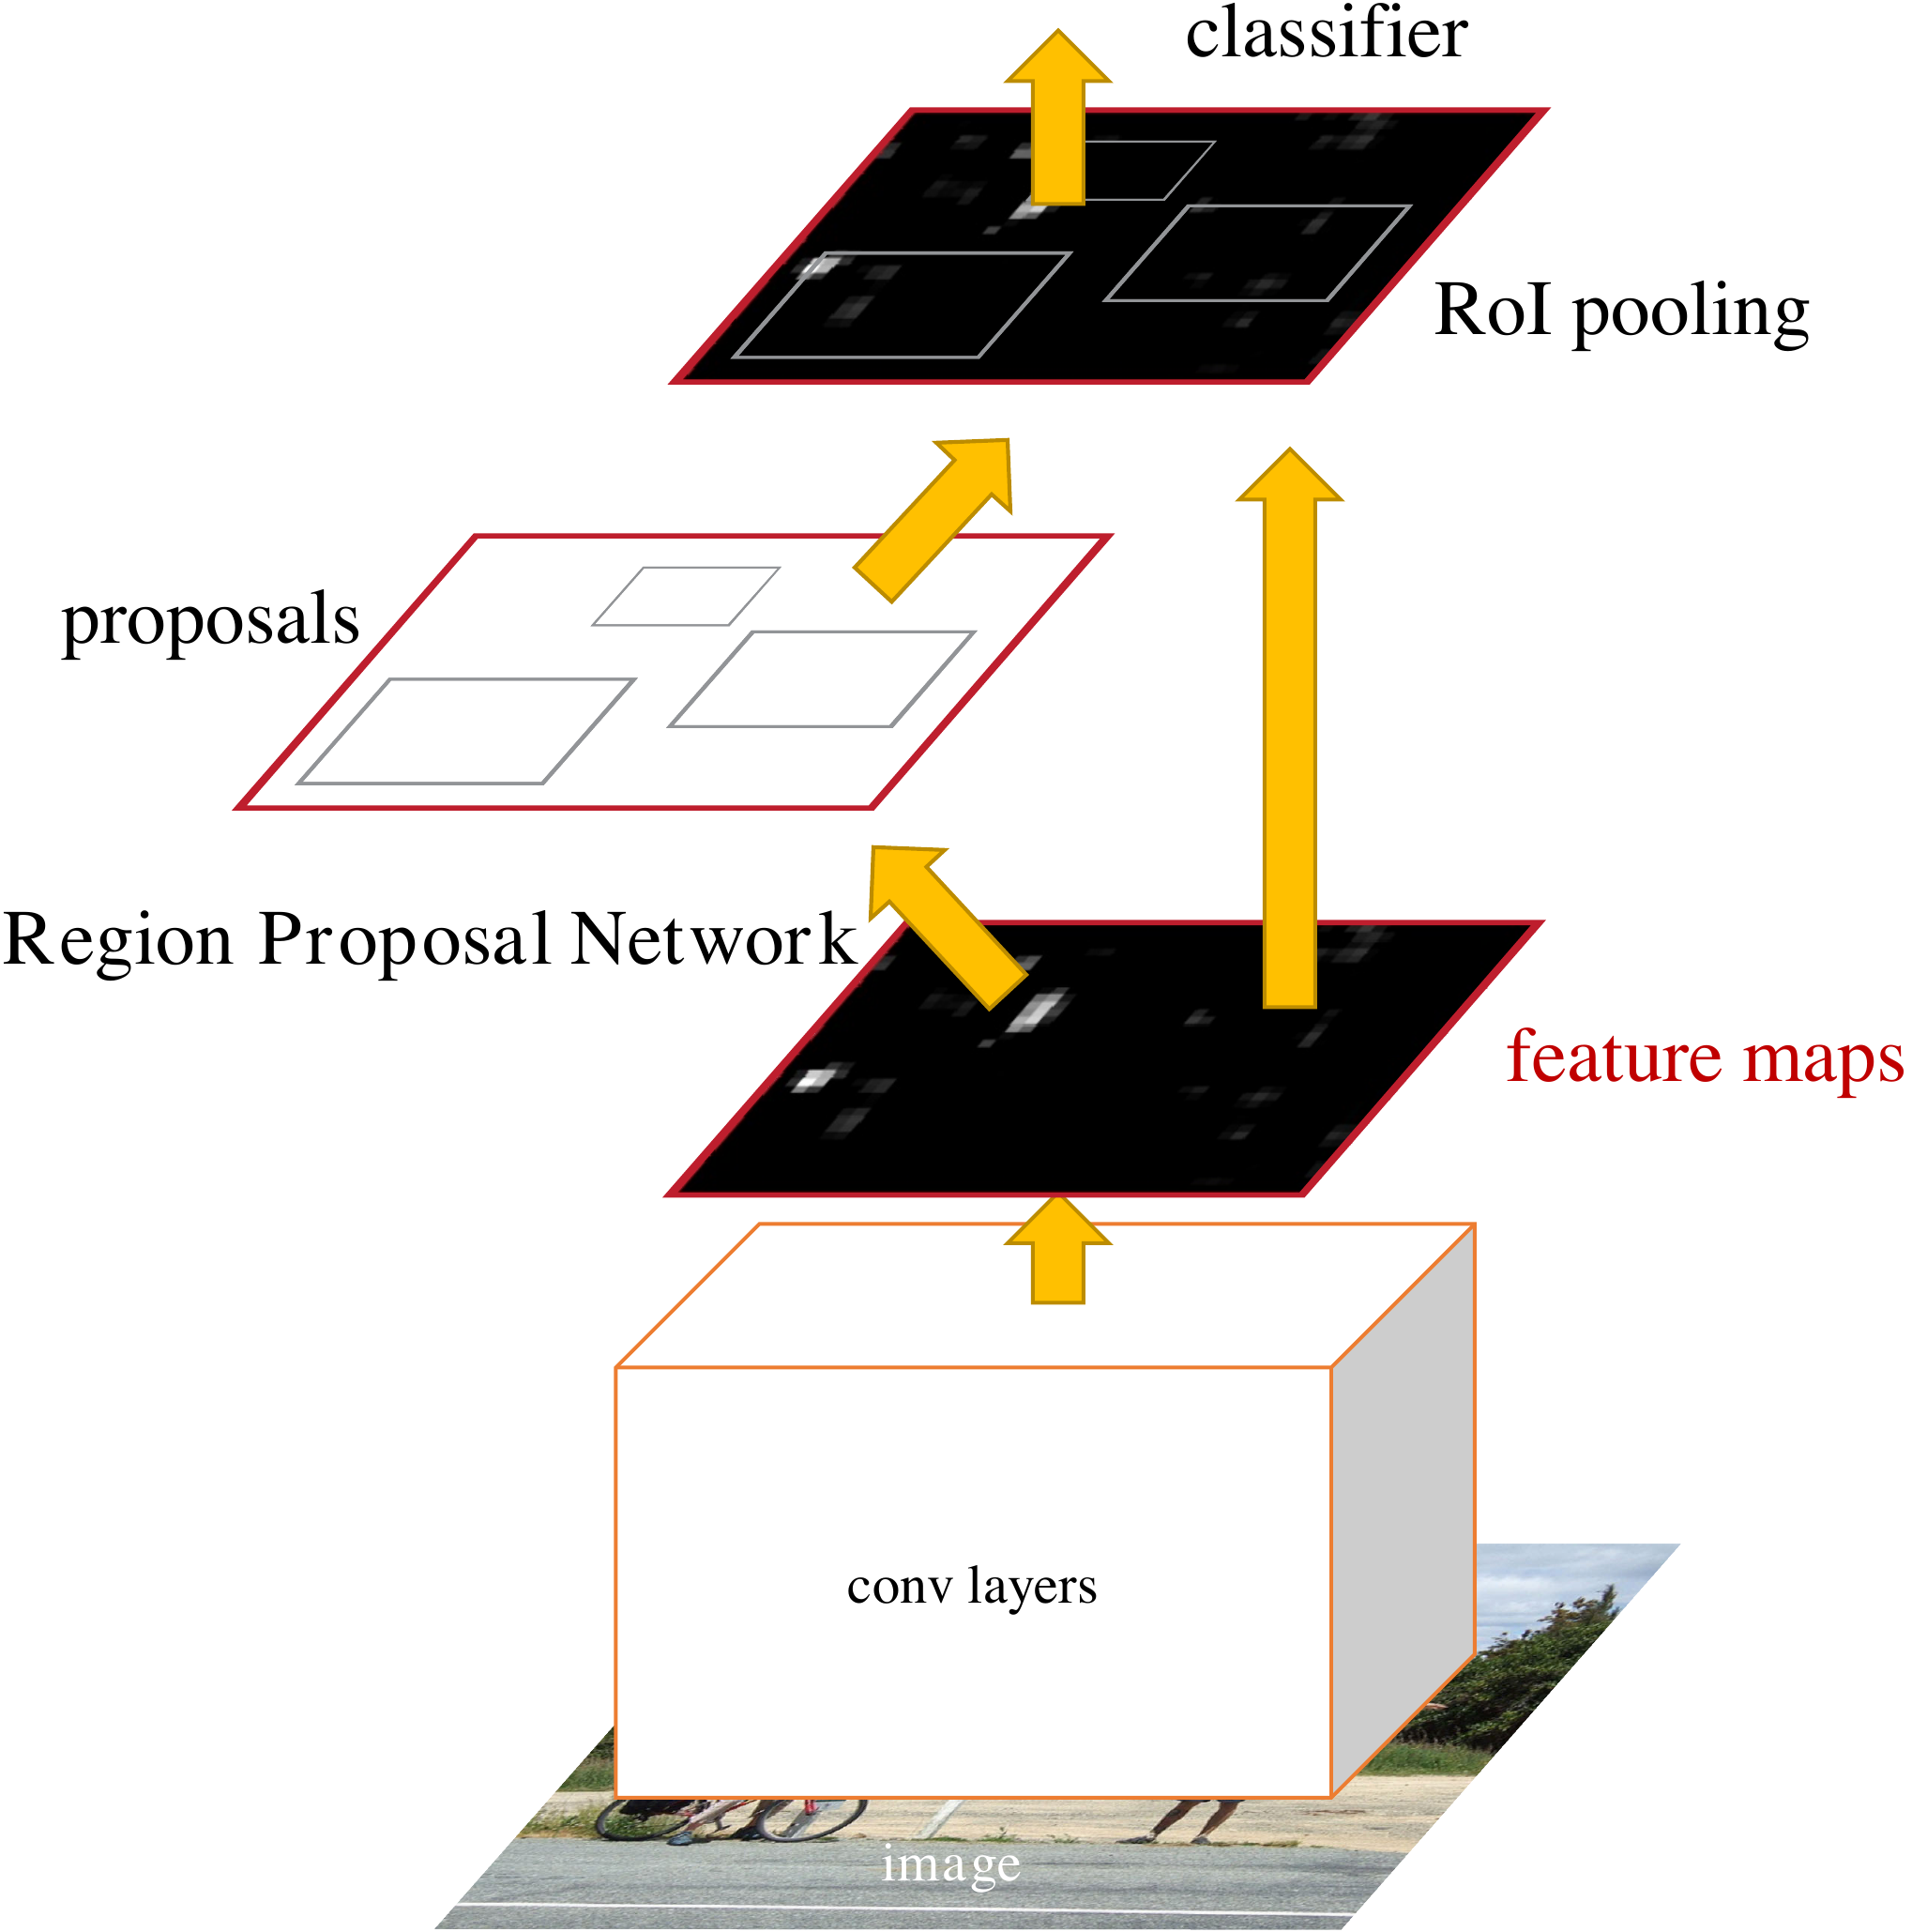
\includegraphics[width=0.5\textwidth]{../figure/fasterrcnn.png}
    \captionsetup{font=footnotesize}
    \bicaption{Faster RCNN 网络\cite{faster_rcnn}}{Faster RCNN Net}
    \label{fig:fasterrcnn}
\end{figure}

Faster R-CNN 的提出使得目标检测算法在高效性和准确性之间取得了更好的平衡。RPN 的引入大大加快了候选区域的生成速度,并且与整个检测网络共享卷积特征图,实现了端到端的训练和检测流程。这使得算法能够实时地处理图像数据,同时保持较高的检测精度,成为目前目标检测领域的主流算法之一,并且为后续的许多目标检测算法提供了基础架构。

Mask R-CNN 是在 Faster R-CNN 的基础上进行了扩展,主要用于同时进行目标检测和实例分割任务。Mask R-CNN 网络结构如图 \ref{fig:maskrcnn} 所示。在 Faster R-CNN 的目标检测框架基础上,Mask R-CNN 额外增加了一个分支网络用于预测每个目标实例的像素级分割掩码。具体来说,在 ROI Pooling 层之后,除了原来的全连接层用于分类和边界框回归外,增加了一个全卷积网络分支来预测目标的分割掩码。该分支网络对每个候选区域生成一个二值掩码,表示该区域内每个像素是否属于目标物体,从而实现对目标物体的精确分割。

\begin{figure}[htbp]
    \centering
    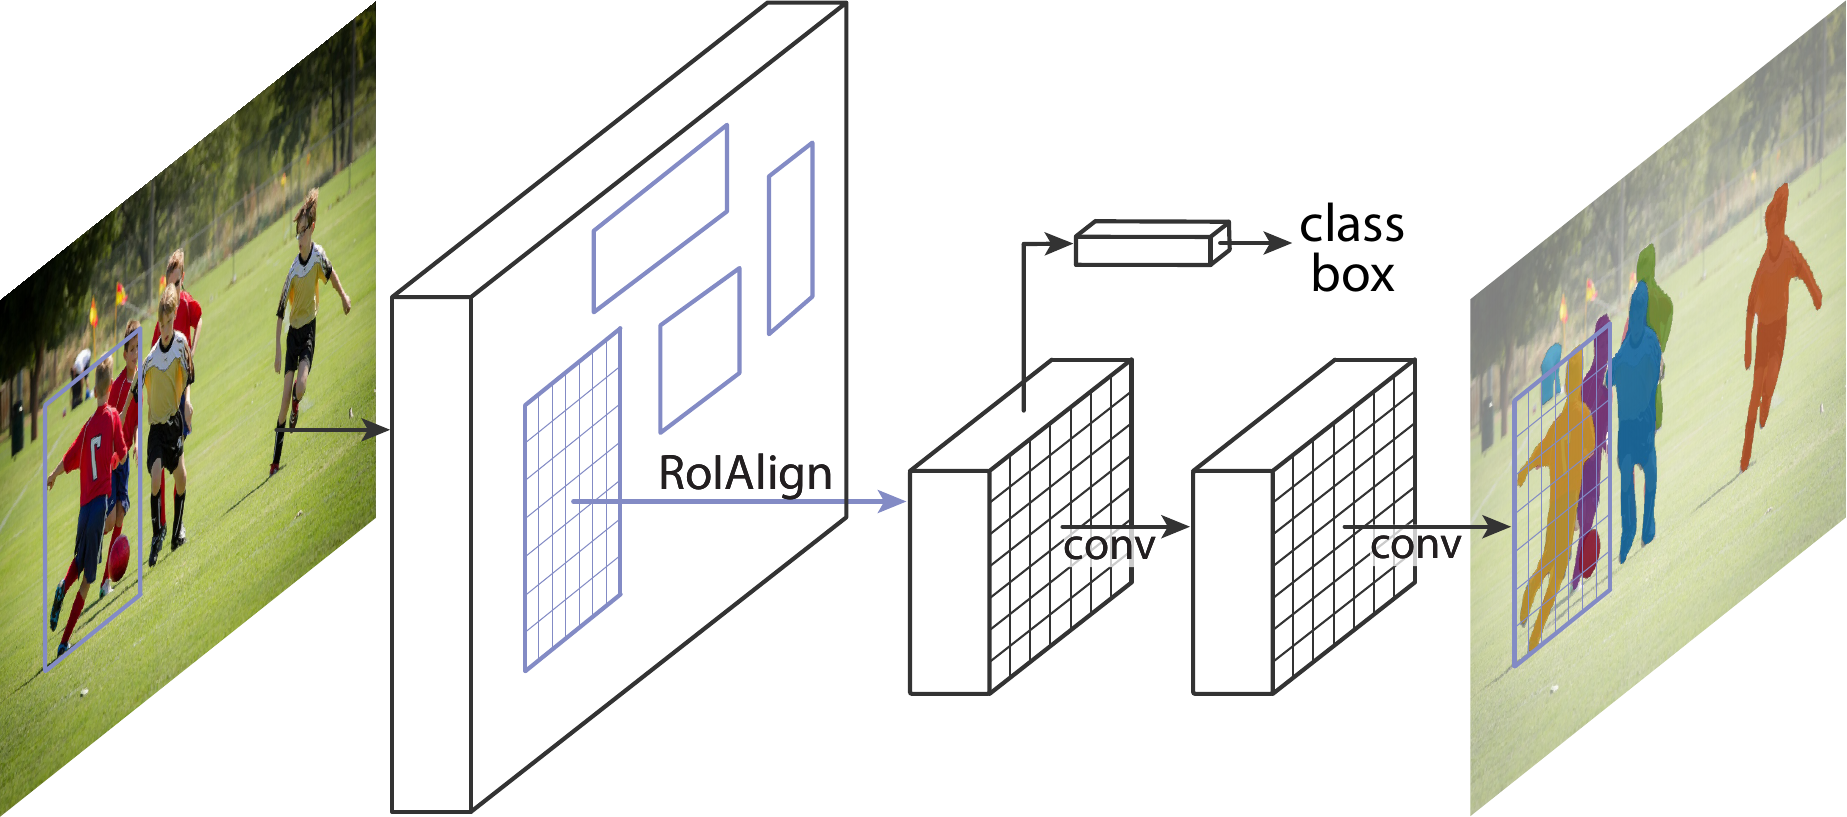
\includegraphics[width=0.7\textwidth]{../figure/maskrcnn.png}
    \captionsetup{font=footnotesize}
    \bicaption{Mask RCNN 网络\cite{mask_rcnn}}{Mask RCNN Net}
    \label{fig:maskrcnn}
\end{figure}

Mask R-CNN 在目标检测和实例分割领域都取得了优异的性能,它不仅能够准确地检测出图像中的目标类别和位置,还能对每个目标物体进行像素级别的分割,为更细粒度的图像理解和分析提供了支持。在诸如医学图像分析、自然场景理解等需要精确分割目标的应用场景中,Mask R-CNN 发挥了重要作用,并且推动了目标检测任务从单纯的边界框定位向更精细化的语义理解方向发展。

尽管在 Fast R-CNN 和 Faster R-CNN 等算法中对计算效率进行了优化,但由于双阶段算法涉及两个阶段的处理,包括候选区域的生成、特征提取、分类识别以及边界框回归等多个步骤,整体计算复杂度仍然较高。在处理高清图像或实时视频流时,可能难以满足实时性的要求,尤其是在资源受限的设备(如移动终端、嵌入式系统等)上,如何进一步降低算法的计算复杂度以实现高效实时的目标检测是一个重要的挑战。例如,在自动驾驶场景中,需要实时处理来自车辆摄像头的大量视频数据,以及时准确地识别道路上的车辆、行人、交通标志等目标,这对算法的实时性提出了极高的要求。

对于图像中的小目标物体,由于其在图像中占据的像素区域较少,特征信息相对有限,在双阶段目标检测算法中容易出现漏检或误检的情况。在候选区域生成阶段,小目标可能由于特征不明显而未被包含在候选区域中;在分类识别阶段,有限的特征信息也难以使模型准确地识别出小目标类别。例如在遥感图像中检测小型建筑物、在显微图像中检测细胞等小目标检测任务中,双阶段算法需要针对小目标的特点进行专门的优化和改进,如采用多层次特征融合策略、设计专门的小目标增强方法等,以提高对小目标的检测性能。

\subsubsection{单阶段目标检测算法}

单阶段目标检测算法摒弃了传统两阶段目标检测算法中先生成候选区域再进行分类识别的繁琐流程,而是将目标分类和定位任务同时进行,直接在图像上进行一次性的预测,从而大大提高了检测速度。其核心思想是将目标检测问题转化为一个端到端的回归问题,输入图像经过深度卷积神经网络的处理后,直接输出目标的类别概率和边界框坐标,这种一体化的处理方式使得单阶段目标检测算法具有较高的实时性和效率。

YOLO 系列\cite{yolov1, yolov2, yolov3, yolov4, yolov6, yolov7, yolov8, yolov9, yolov10, yolov11}算法作为单阶段目标检测算法的重要分支,基于深度学习的卷积神经网络构建其检测模型。卷积神经网络通过卷积层、池化层、激活函数等结构对图像进行特征提取和非线性变换,学习到图像的层次化特征表示。YOLO 网络结构如图 \ref{fig:yolov1} 所示。在 YOLO 算法中,网络将输入图像划分为多个大小相等的网格(grid cell),每个网格负责预测一定数量的边界框(bounding box)以及该边界框内包含目标物体的类别概率和边界框坐标。边界框的坐标通常包括边界框的中心坐标、宽度和高度等信息,而类别概率则表示该边界框内属于每个目标类别的可能性。

\begin{figure}[htbp]
    \centering
    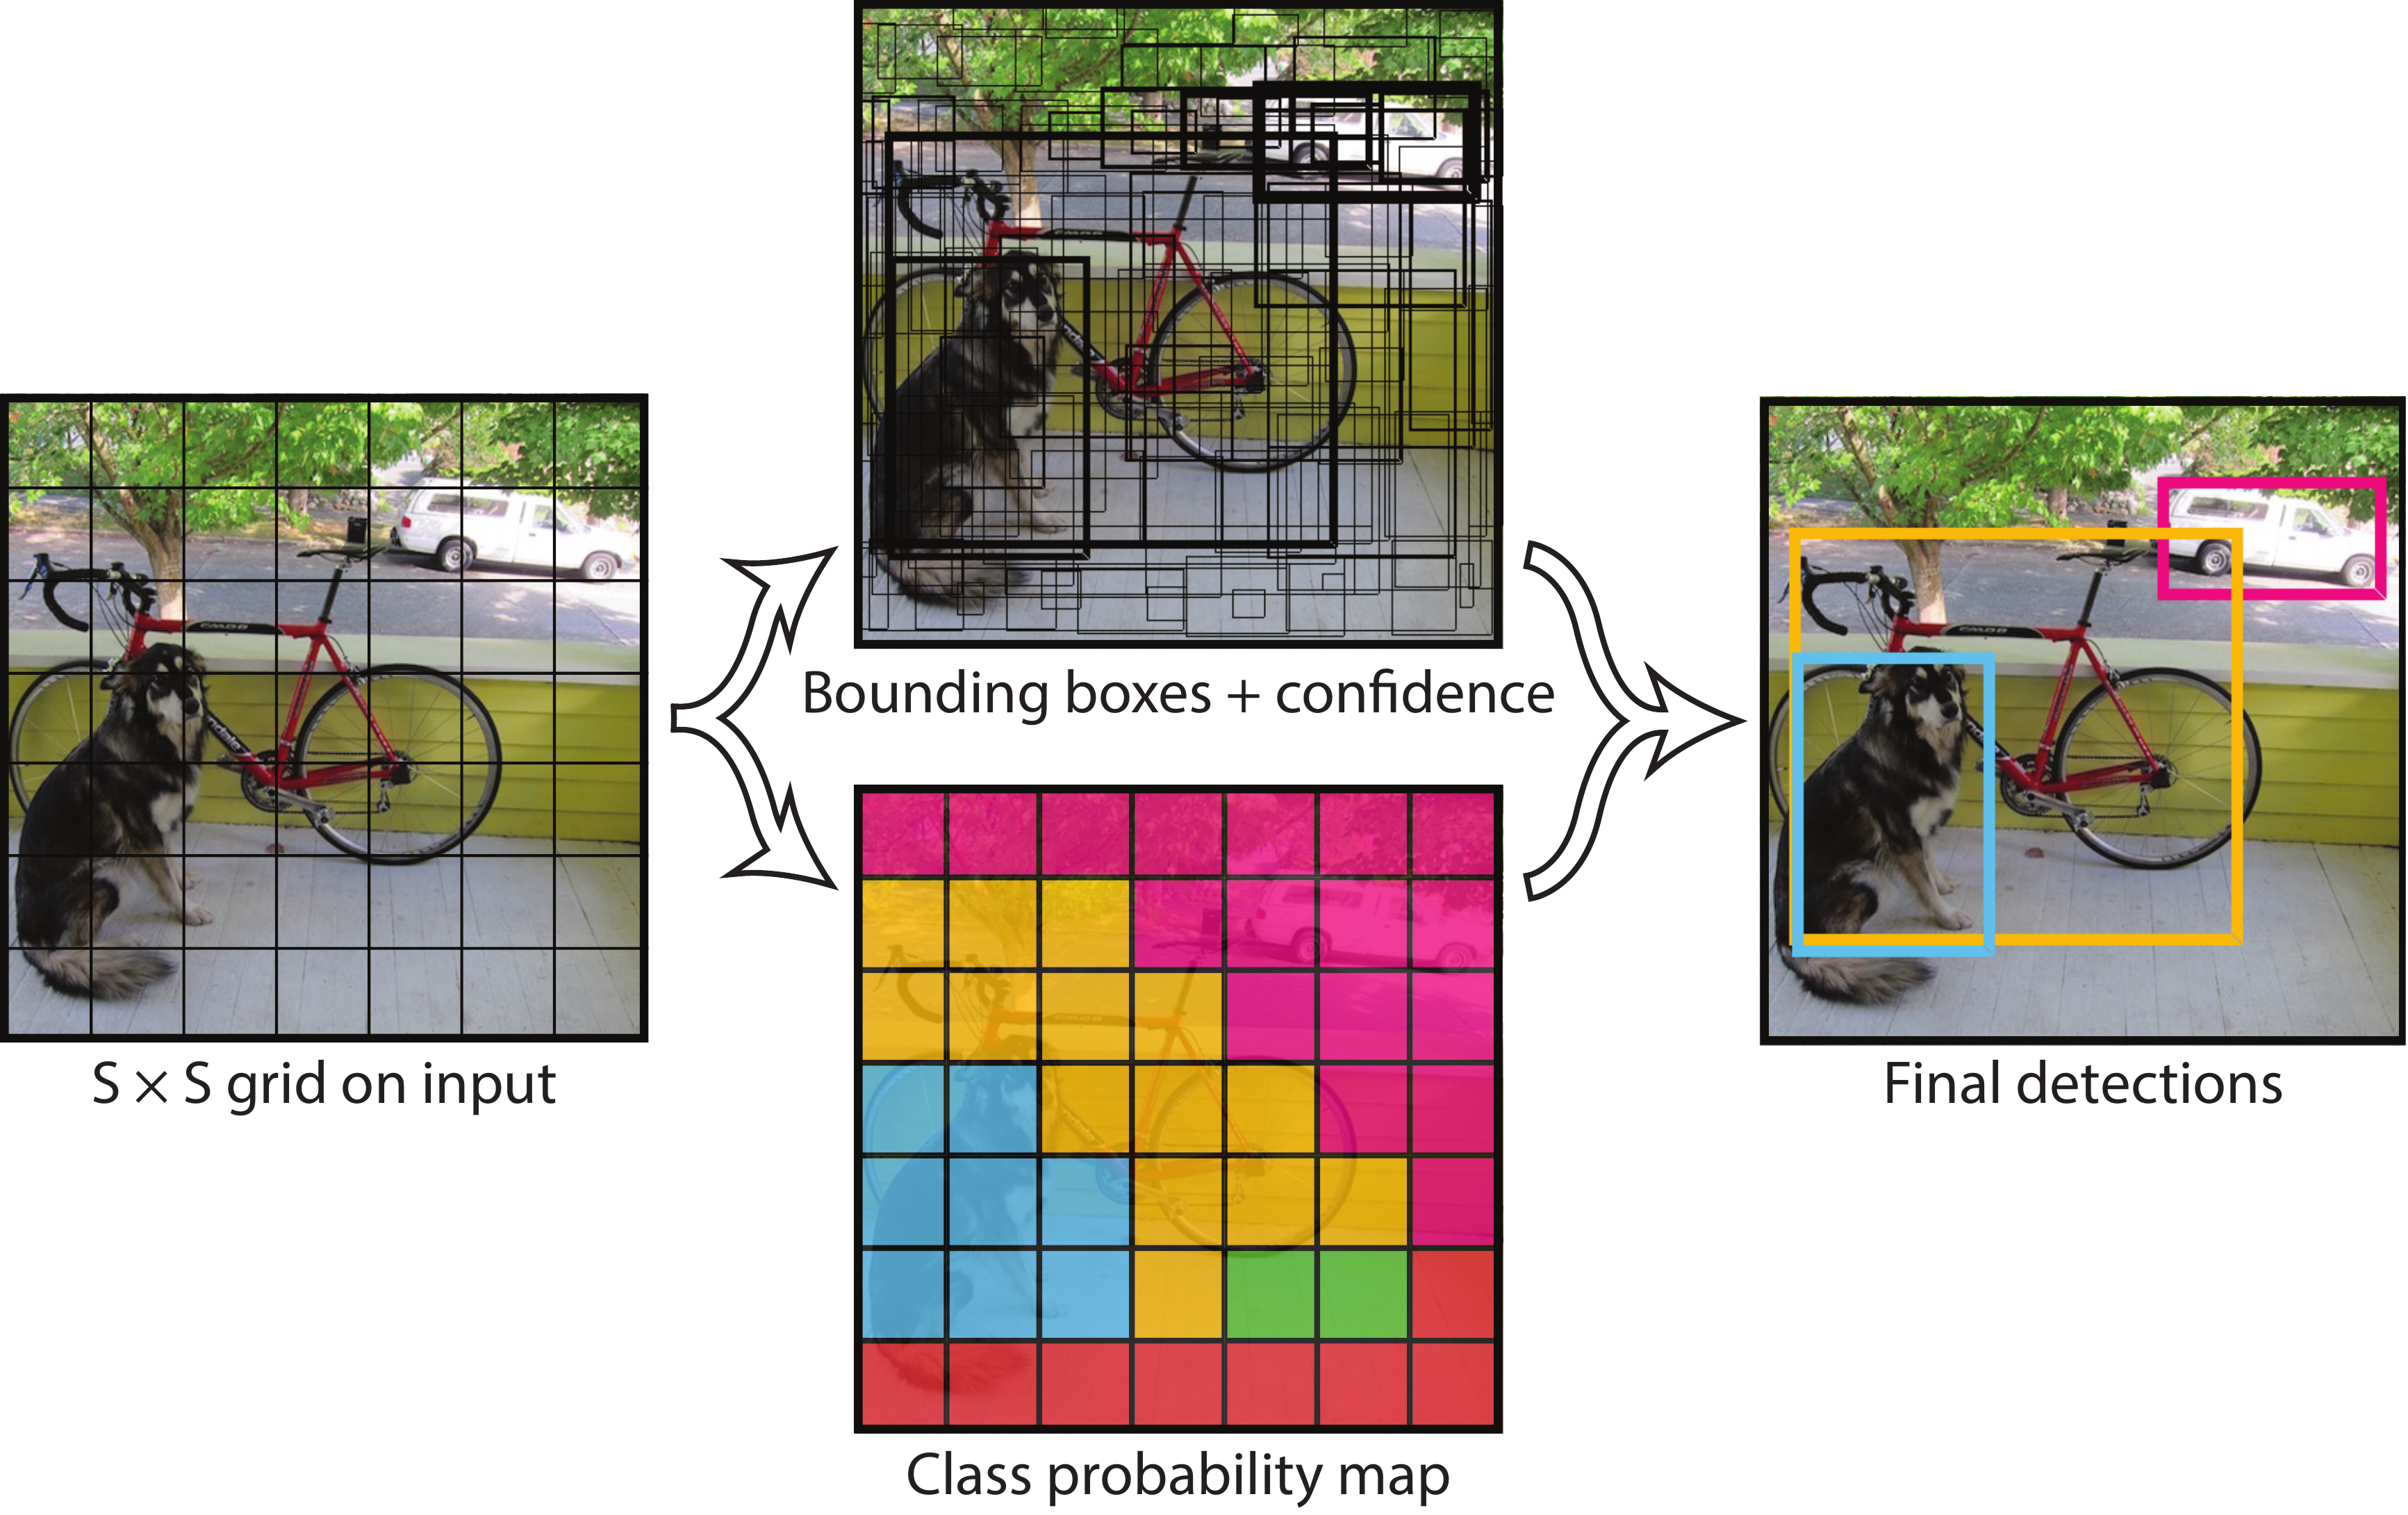
\includegraphics[width=0.7\textwidth]{../figure/yolov1.png}
    \captionsetup{font=footnotesize}
    \bicaption{YOLO 网络\cite{yolov1}}{YOLO Net}
    \label{fig:yolov1}
\end{figure}

在训练过程中,YOLO 系列算法采用监督学习的方式,利用标注有目标类别和边界框的训练数据对模型进行训练。通过定义损失函数,将预测的边界框坐标和类别概率与真实值之间的误差进行度量,并利用反向传播算法不断调整网络的参数,使得模型能够学习到准确的目标检测特征和知识,从而在测试时对新的图像进行快速、准确的目标检测。YOLOv4 网络结构如图 \ref{fig:yolov4} 所示。

\begin{figure}[htbp]
    \centering
    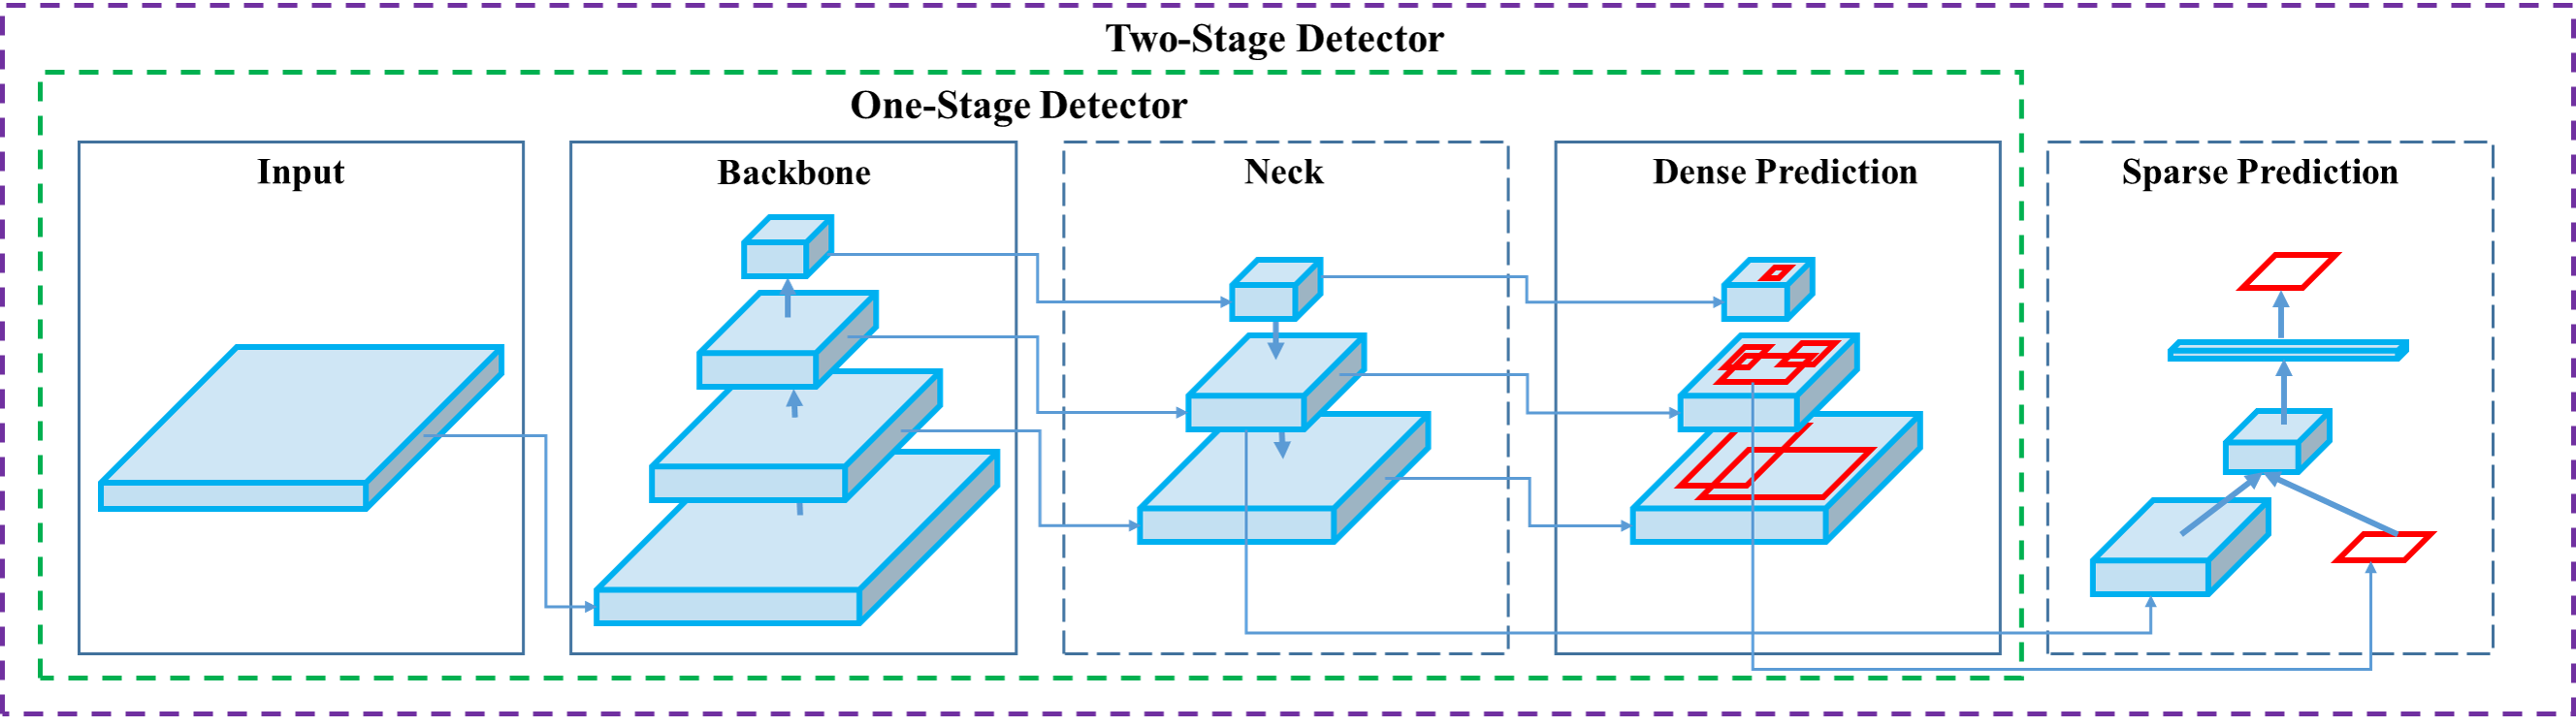
\includegraphics[width=0.8\textwidth]{../figure/yolov4.png}
    \captionsetup{font=footnotesize}
    \bicaption{YOLOv4 网络\cite{yolov4}}{YOLOv4 Net}
    \label{fig:yolov4}
\end{figure}

YOLOv5 以其简洁高效的特点,在工业界得到了广泛的应用和推广。它对 YOLO 系列算法进行了进一步的简化和优化,使其更易于部署和使用。
YOLOv5 在网络结构上进行了调整,采用了更少的参数量和计算量,同时保持了较高的检测精度。它引入了一种新的 PANet(Path Aggregation Network)结构\cite{pan},优化了特征融合的方式,使得特征信息能够更有效地在不同尺度之间传递和共享。此外,YOLOv5 还提供了多种不同规模的模型版本,以满足不同应用场景下对速度和精度的平衡需求。
YOLOv5 的出现大大降低了 YOLO 算法在实际工业应用中的部署门槛,使得更多的企业能够快速地将目标检测技术应用于产品开发和生产过程中,如智能安防、智能交通等领域。

在 YOLOv5 之后,YOLO 系列又相继推出了 YOLOv6、YOLOv7 和 YOLOv8 等版本。这些版本在前作的基础上不断进行改进和创新。
YOLOv6 专注于提高模型的效率和实时性,在移动端等资源受限设备上的表现尤为突出。它采用了更轻量化的网络结构和优化算法,进一步降低了模型的计算复杂度,同时通过一系列的优化技巧,如量化感知训练等,确保了模型在低精度硬件上的性能。
YOLOv7 则在速度和精度的平衡方面取得了新的突破,提出了一些新颖的架构设计和训练策略,使得模型能够在保持较高速度的同时,进一步提升检测精度,为高精度目标检测任务提供了更好的解决方案。
YOLOv8 改进的注意力机制和更先进的特征融合方法等。YOLOv8 在模型的易用性、灵活性以及性能方面都有显著的提升,能够适应各种不同的目标检测任务和应用场景。YOLOv8 网络结构如图 \ref{fig:yolov8} 所示。

\begin{figure}[htbp]
    \centering
    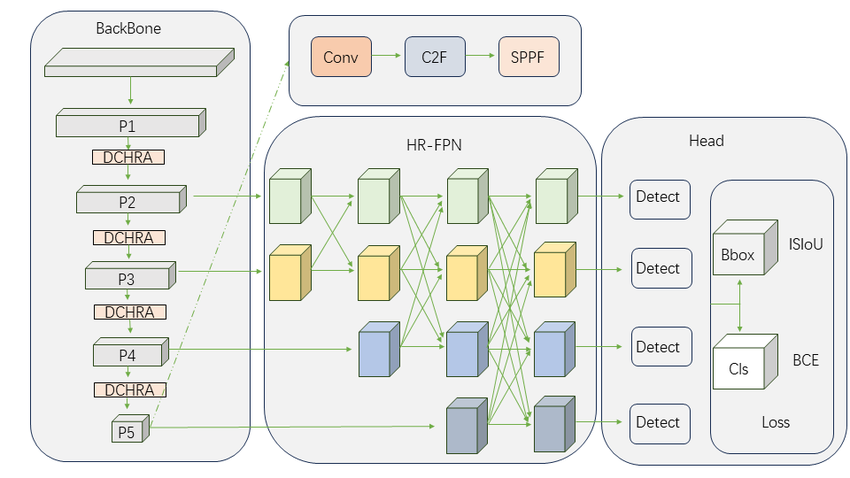
\includegraphics[width=0.8\textwidth]{../figure/yolov8.png}
    \captionsetup{font=footnotesize}
    \bicaption{YOLOv8 网络\cite{yolov8}}{YOLOv8 Net}
    \label{fig:yolov8}
\end{figure}

YOLO 系列算法作为单阶段目标检测算法的代表,其最大的优势在于能够实现实时、快速的目标检测。通过将目标检测任务转化为端到端的回归问题,省去了候选区域生成和特征提取的中间步骤,大大提高了检测速度。例如,YOLOv4 在常见的 GPU 设备上可以达到每秒数十帧甚至更高的检测速度,能够满足实时视频监控、自动驾驶等对实时性要求较高的应用场景的需求。

随着 YOLO 系列算法的不断演进,其检测精度也在不断提高。从 YOLOv1 到 YOLOv5,通过引入锚框机制、多尺度预测、改进的特征提取网络等技术手段,YOLO 系列算法在各种目标检测数据集上的平均精度均值(mAP)等性能指标上取得了显著的提升,能够准确地识别和定位图像中的目标物体,即使在复杂场景下也能保持较好的检测效果。

虽然 YOLO 系列算法在整体检测精度上取得了较好的成绩,但对于图像中的小目标物体,其检测精度仍然存在一定的提升空间。小目标物体由于在图像中占据的像素区域较少,特征信息有限,容易受到背景噪声和其他物体的干扰,导致 YOLO 算法在检测小目标时出现漏检或误检的情况。例如,在航拍图像中的行人检测、显微图像中的细胞检测等场景中,小目标检测的准确性仍然是 YOLO 系列算法需要进一步解决的难题。

在追求更高检测速度和精度的过程中,YOLO 系列算法需要在模型复杂度、计算资源消耗以及检测性能之间进行优化和平衡。随着模型深度和复杂度的增加,虽然检测精度可能会有所提高,但计算量和内存占用也会随之增大,这可能会导致算法在资源受限的设备上无法高效运行,甚至无法部署。因此,如何在保证检测性能的前提下,通过模型压缩、剪枝、量化等技术手段对 YOLO 系列算法进行优化,以适应不同硬件平台的性能要求,是当前 YOLO 系列算法发展面临的一个重要挑战。


\subsection{图像去雾还原的理论基础与算法}

\subsubsection{传统的图像去雾算法相关研究}

于晴朗天气下,场景中的物体光线能近乎直接、完整地抵达成像设备传感器,所获图像清晰且色彩精准。然雾天环境则截然不同,大气中的水汽凝结成微小水滴,悬浮于空气之中,其数量密度随雾浓度递增。当物体发出或反射的光线在传播途中,遭遇这些水滴时,便发生复杂的散射现象。
从光学层面而言,光线与雾粒子的相互作用遵循米氏散射理论。水滴尺寸与可见光波长相当,故米氏散射效应显著。入射光线在水滴表面发生散射,散射光强分布呈各向异性,部分光线偏离原传播方向,无法顺利抵达传感器。这就直接导致了场景中远处物体大量光线被散射损耗,成像时亮度信息弱化,图像整体暗淡且对比度严重下滑。不仅如此,不同波长光线散射程度有别,短波长的蓝光散射更为剧烈,使得雾天图像普遍呈现出偏蓝、偏灰的灰雾色调,色彩失真明显。

大气散射模型如图 \ref{dehaze} 所示。大气散射模型精准地数学化描述了雾天成像过程。其核心表达式为:
\begin{equation}
    \label{eq:haze2}
    I(x) = J(x)t(x)+A(1-t(x))
\end{equation}

公式\ref{eq:haze2}中,$I(x)$ 表示成像设备捕获的雾天图像某一点的观测强度;$J(x)$ 是该场景点在无雾状态下的真实场景辐射强度,蕴含着物体本来的颜色、纹理等关键信息;$t(x)$ 为大气透射率,衡量光线从场景点传播至传感器过程中,未被大气介质散射丢失的能量比例,其值介于 0 到 1 之间;$A$ 是大气光照,在均匀浓雾场景近似为常数,代表大气散射引入的背景光照强度,常呈现为灰白色调。
该模型直观展现了雾天图像退化根源:场景辐射光受大气阻碍衰减,同时大气散射光叠加其上。透射率 $t(x)$ 与大气光照 $A$ 成为模型两大关键参数,二者与雾浓度紧密关联且呈反向变化趋势。雾愈浓,透射率愈低,散射光干扰愈强,图像偏离真实场景愈远。

\begin{figure}[htbp]
    \centering
    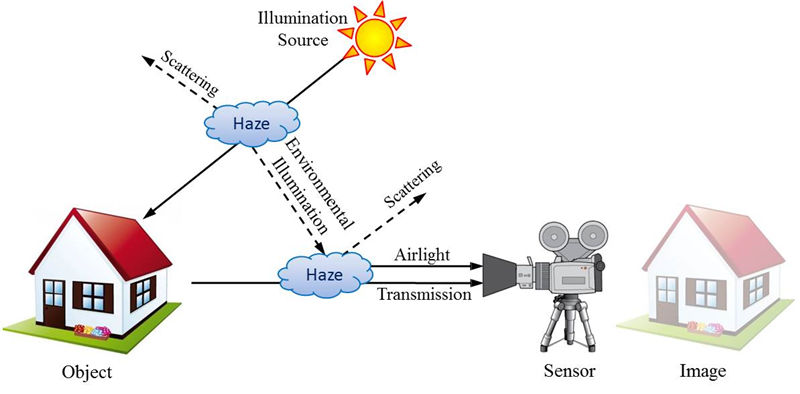
\includegraphics[width=0.8\textwidth]{../figure/dehaze.png}
    \captionsetup{font=footnotesize}
    \bicaption{大气散射模型\cite{cai2016dehazenet}}{Atmospheric Ejection Model.}
    \label{fig:dehaze}
\end{figure}

暗通道先验理论是图像去雾领域的重要突破。该理论基于在无雾自然图像的局部区域内,至少存在一种颜色通道(红、绿、蓝中的一个)具有非常低的像素强度这一观察结果。在无雾图像的局部区域中,往往存在一些没有被明亮光照直接照射到的暗区域,这些区域在某一颜色通道上的值会非常小,接近于零。在有雾图像中,由于雾的存在,这些暗区域的像素强度会被抬高,从而可以通过寻找图像中暗通道的最小值来估计大气光照,并进一步计算出传输系数。暗通道先预理论为图像去雾提供了一种有效的估计方法,具有计算效率高、对复杂场景适应性强等优点。但需要注意的是,暗通道先预在某些特定场景,如包含大面积亮白色物体或特殊光照条件的图像中,可能会出现估计误差,导致去雾效果不理想。

早期的基于物理模型的去雾算法主要依赖于对大气散射模型参数的手动估计,例如通过参考场景中的已知物体颜色或亮度来估计大气光照和传输系数。然而,手动估计参数的方法在实际应用中效率低下且准确性难以保证。随后,研究者们提出了一些基于物理模型的自动估计方法。例如,利用天空区域的特性来估计大气光照,假设天空区域的像素强度接近于大气光照强度,并通过图像分割技术提取天空区域进行估计。对于传输系数的估计,一些方法基于场景深度信息或散射系数的先验知识进行建模,如利用地形数据库或激光雷达测量数据来获取场景深度,进而计算传输系数。这类基于物理模型的方法在理论上有较强的物理意义,但在实际应用中往往对先验信息的依赖度较高,且计算复杂度较大,难以实时处理大规模图像数据。


图像处理相关理论也为图像去雾提供了支持。图像的对比度增强技术可以改善雾天图像的视觉效果,通过拉伸图像的灰度级范围,使图像中的暗细节更加清晰,但单纯的对比度增强并不能消除雾天图像中的散射光成分。图像的多尺度分析方法则可以从不同尺度上对图像进行分解和处理,有利于在去雾过程中同时保留图像的全局结构信息和局部细节特征。此外,图像的先验知识,如图像的边缘信息、纹理信息等,也可以作为约束条件融入到去雾算法中,以提高去雾的精度和质量。

基于图像处理的去雾算法不直接依赖于大气散射模型,而是通过对图像的像素强度、颜色分布、纹理等特征进行分析和处理来实现去雾效果。常见的基于图像处理的去雾算法包括基于图像对比度增强的方法、基于滤波的方法等。

基于图像对比度增强的方法通过对图像的灰度级或颜色通道进行拉伸、均衡化等操作,来提高图像的对比度,从而改善雾天图像的能见度。例如,直方图均衡化技术是一种简单而常用的对比度增强方法,它通过调整图像像素的分布,使图像的灰度级范围更加均匀,从而增强图像的对比度。然而,单纯的对比度增强方法可能会导致图像的色彩失真,且无法有效去除图像中的散射光成分。

基于滤波的方法则利用滤波器对图像进行处理,以提取图像中的有用信息并抑制雾的影响。高通滤波器可以突出图像中的高频细节信息,如边缘、纹理等,而低通滤波器则可以平滑图像中的噪声和模糊成分。一些去雾算法将高通滤波和低通滤波相结合,通过在不同频域上对图像进行处理来实现去雾效果。例如,通过高通滤波提取图像的细节信息,然后将其与经过低通滤波处理后的图像进行融合,以恢复出清晰的图像。此外,还有一些基于自适应滤波的去雾方法,可以根据图像局部区域的特性自动调整滤波器的参数,以更好地适应不同场景下的去雾需求。但基于滤波的去雾算法也可能存在一些问题,如滤波器的设计和参数选择对去雾效果影响较大,且在处理复杂图像时可能会出现伪影等现象。

传统图像去雾算法在理论和实践中都取得了一定的成果,但它们也存在一些局限性。基于物理模型的方法对先验信息的依赖性强,且计算复杂度较高;基于图像处理的方法虽然计算效率相对较高,但在去雾精度和效果上可能不如基于物理模型的方法。随着计算机视觉技术和机器学习技术的不断发展,新的图像去雾算法不断涌现,这些新算法在一定程度上克服了传统算法的不足,为图像去雾技术的发展带来了新的机遇和挑战。

\subsubsection{基于深度学习的图像去雾算法相关研究}

深度学习技术以其强大的特征自动学习能力,在图像去雾领域展现出独特的优势。传统的图像去雾方法往往依赖于人工设计的特征提取和先验知识,处理复杂场景时存在局限性。而深度学习模型,尤其是卷积神经网络(CNN),能够自动从大量带有雾和无雾的图像数据中学习到丰富的特征表示。这些特征涵盖了从低层的纹理、边缘信息到高层的语义信息,使得模型在面对多样化的雾天图像时,能够更精准地理解场景内容和雾的影响模式。例如,在城市街景图像去雾中,深度学习模型可以自动识别出建筑物、道路、车辆等不同物体的特征,并针对性地进行去雾处理,恢复出清晰的图像结构。此外,深度学习模型具有良好的泛化能力,经过充分训练后,能够在不同光照条件、不同雾浓度以及不同场景类型的图像上保持相对稳定的去雾效果。

端到端的卷积神经网络去雾算法以雾天图像作为输入,直接输出对应的无雾图像。其核心在于构建一个深度卷积神经网络模型,该模型通过大量的带有雾和无雾图像对进行训练,自动学习雾天图像与无雾图像之间的复杂非线性映射关系。在网络训练过程中,卷积神经网络的多层卷积结构能够自动提取图像的特征,从低层的边缘、纹理等基本特征到高层的语义特征。这些特征对于理解和恢复图像中的场景内容以及去除雾的影响至关重要。例如,卷积层中的卷积核可以看作是特征提取器,通过与图像进行卷积操作,生成特征图,突出图像中与去雾相关的特定模式和结构。池化层则用于降低特征图的维度,减少计算量的同时保留关键特征信息,增强模型对图像尺度变化的适应性。

在网络的反向传播过程中,通过定义合适的损失函数,如均方误差损失(MSE)或结构相似性损失(SSIM),来衡量生成的无雾图像与真实无雾图像之间的差异。模型根据损失函数的反馈,自动调整网络中的权重参数,使得网络不断学习和优化特征提取与映射能力,最终达到准确去雾的目的。

DehazeNet\cite{cai2016dehazenet} 是早期具有代表性的基于卷积神经网络的端到端去雾算法。DehazeNet 网络结构如图 \ref{fig:dehazenet} 所示。它采用了多层卷积结构,专门设计用于估计大气散射模型中的传输系数。DehazeNet 的网络结构相对简单,但有效。它通过三个卷积层逐步提取雾天图像的特征,并利用这些特征来估计传输系数,进而根据大气散射模型恢复出无雾图像。该算法首次将深度学习技术应用于图像去雾领域,并取得了一定的成果,在一些常见的图像去雾数据集上表现出了较好的性能,为后续基于深度学习的去雾研究奠定了基础。然而,DehazeNet 也存在一些局限性,例如模型参数较多,导致计算复杂度较高,训练和测试速度较慢,在处理大规模图像数据时效率较低。

\begin{figure}[htbp]
    \centering
    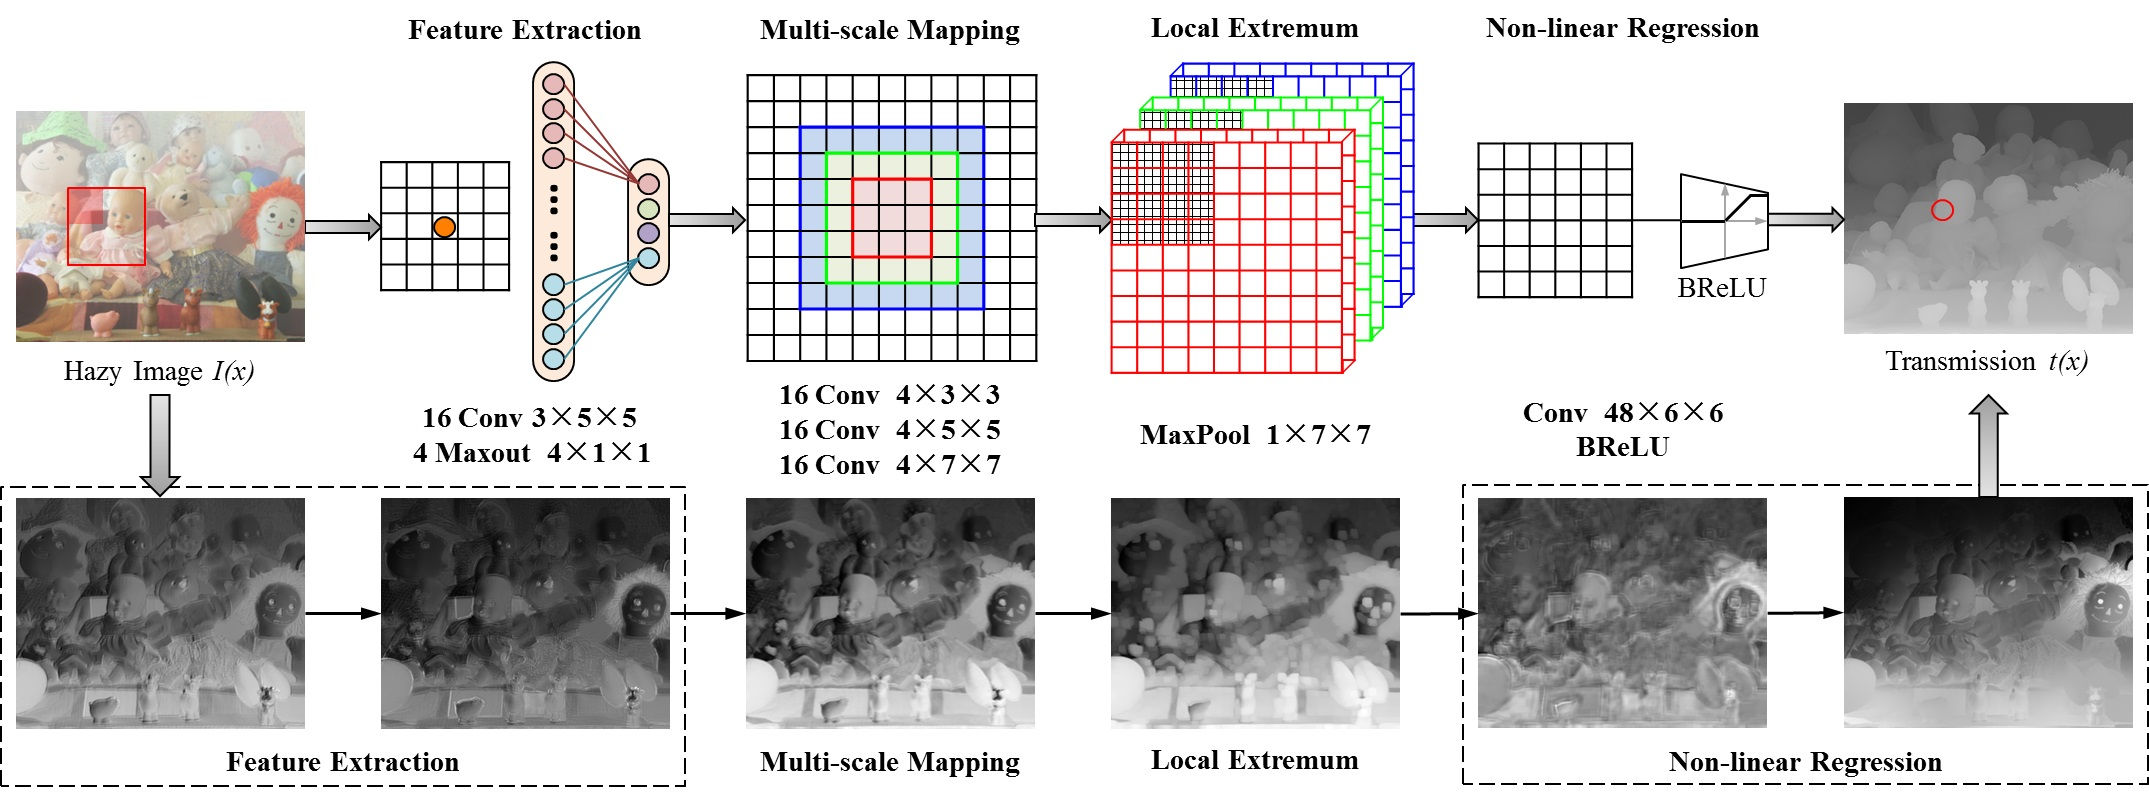
\includegraphics[width=0.9\textwidth]{../figure/hazenet.png}
    \captionsetup{font=footnotesize}
    \bicaption{DeHaze 网络\cite{cai2016dehazenet}}{DeHaze Net}
    \label{fig:dehazenet}
\end{figure}

为了解决 DehazeNet 等早期算法存在的问题,AOD-Net 应运而生。AOD-Net 提出了一种更紧凑的网络架构,将大气散射模型的逆过程融入到网络中,能够同时估计大气光照和传输系数。AOD-Net 网络结构如图 \ref{fig:aodnet} 所示。其网络结构主要包括一个编码器和一个解码器。编码器部分通过卷积层和池化层提取图像的多尺度特征,逐步降低特征图的空间维度,同时增加通道数,提取更抽象的特征。解码器部分则通过反卷积层或上采样层将编码器提取的特征逐步恢复到与输入图像相同的空间维度,生成对应的无雾图像。AOD-Net 引入了残差学习思想,在网络的每一层都学习输入与输出之间的残差,使得网络更容易训练,能够更快地收敛,并且有效地缓解了梯度消失问题。实验表明,AOD-Net 在多个公开数据集上的去雾性能优于以往的传统方法和一些早期的深度学习方法,能够生成更清晰、自然的无雾图像,并且在计算速度上有显著提升,具有较好的实时性。

\begin{figure}[ht]
    \centering
    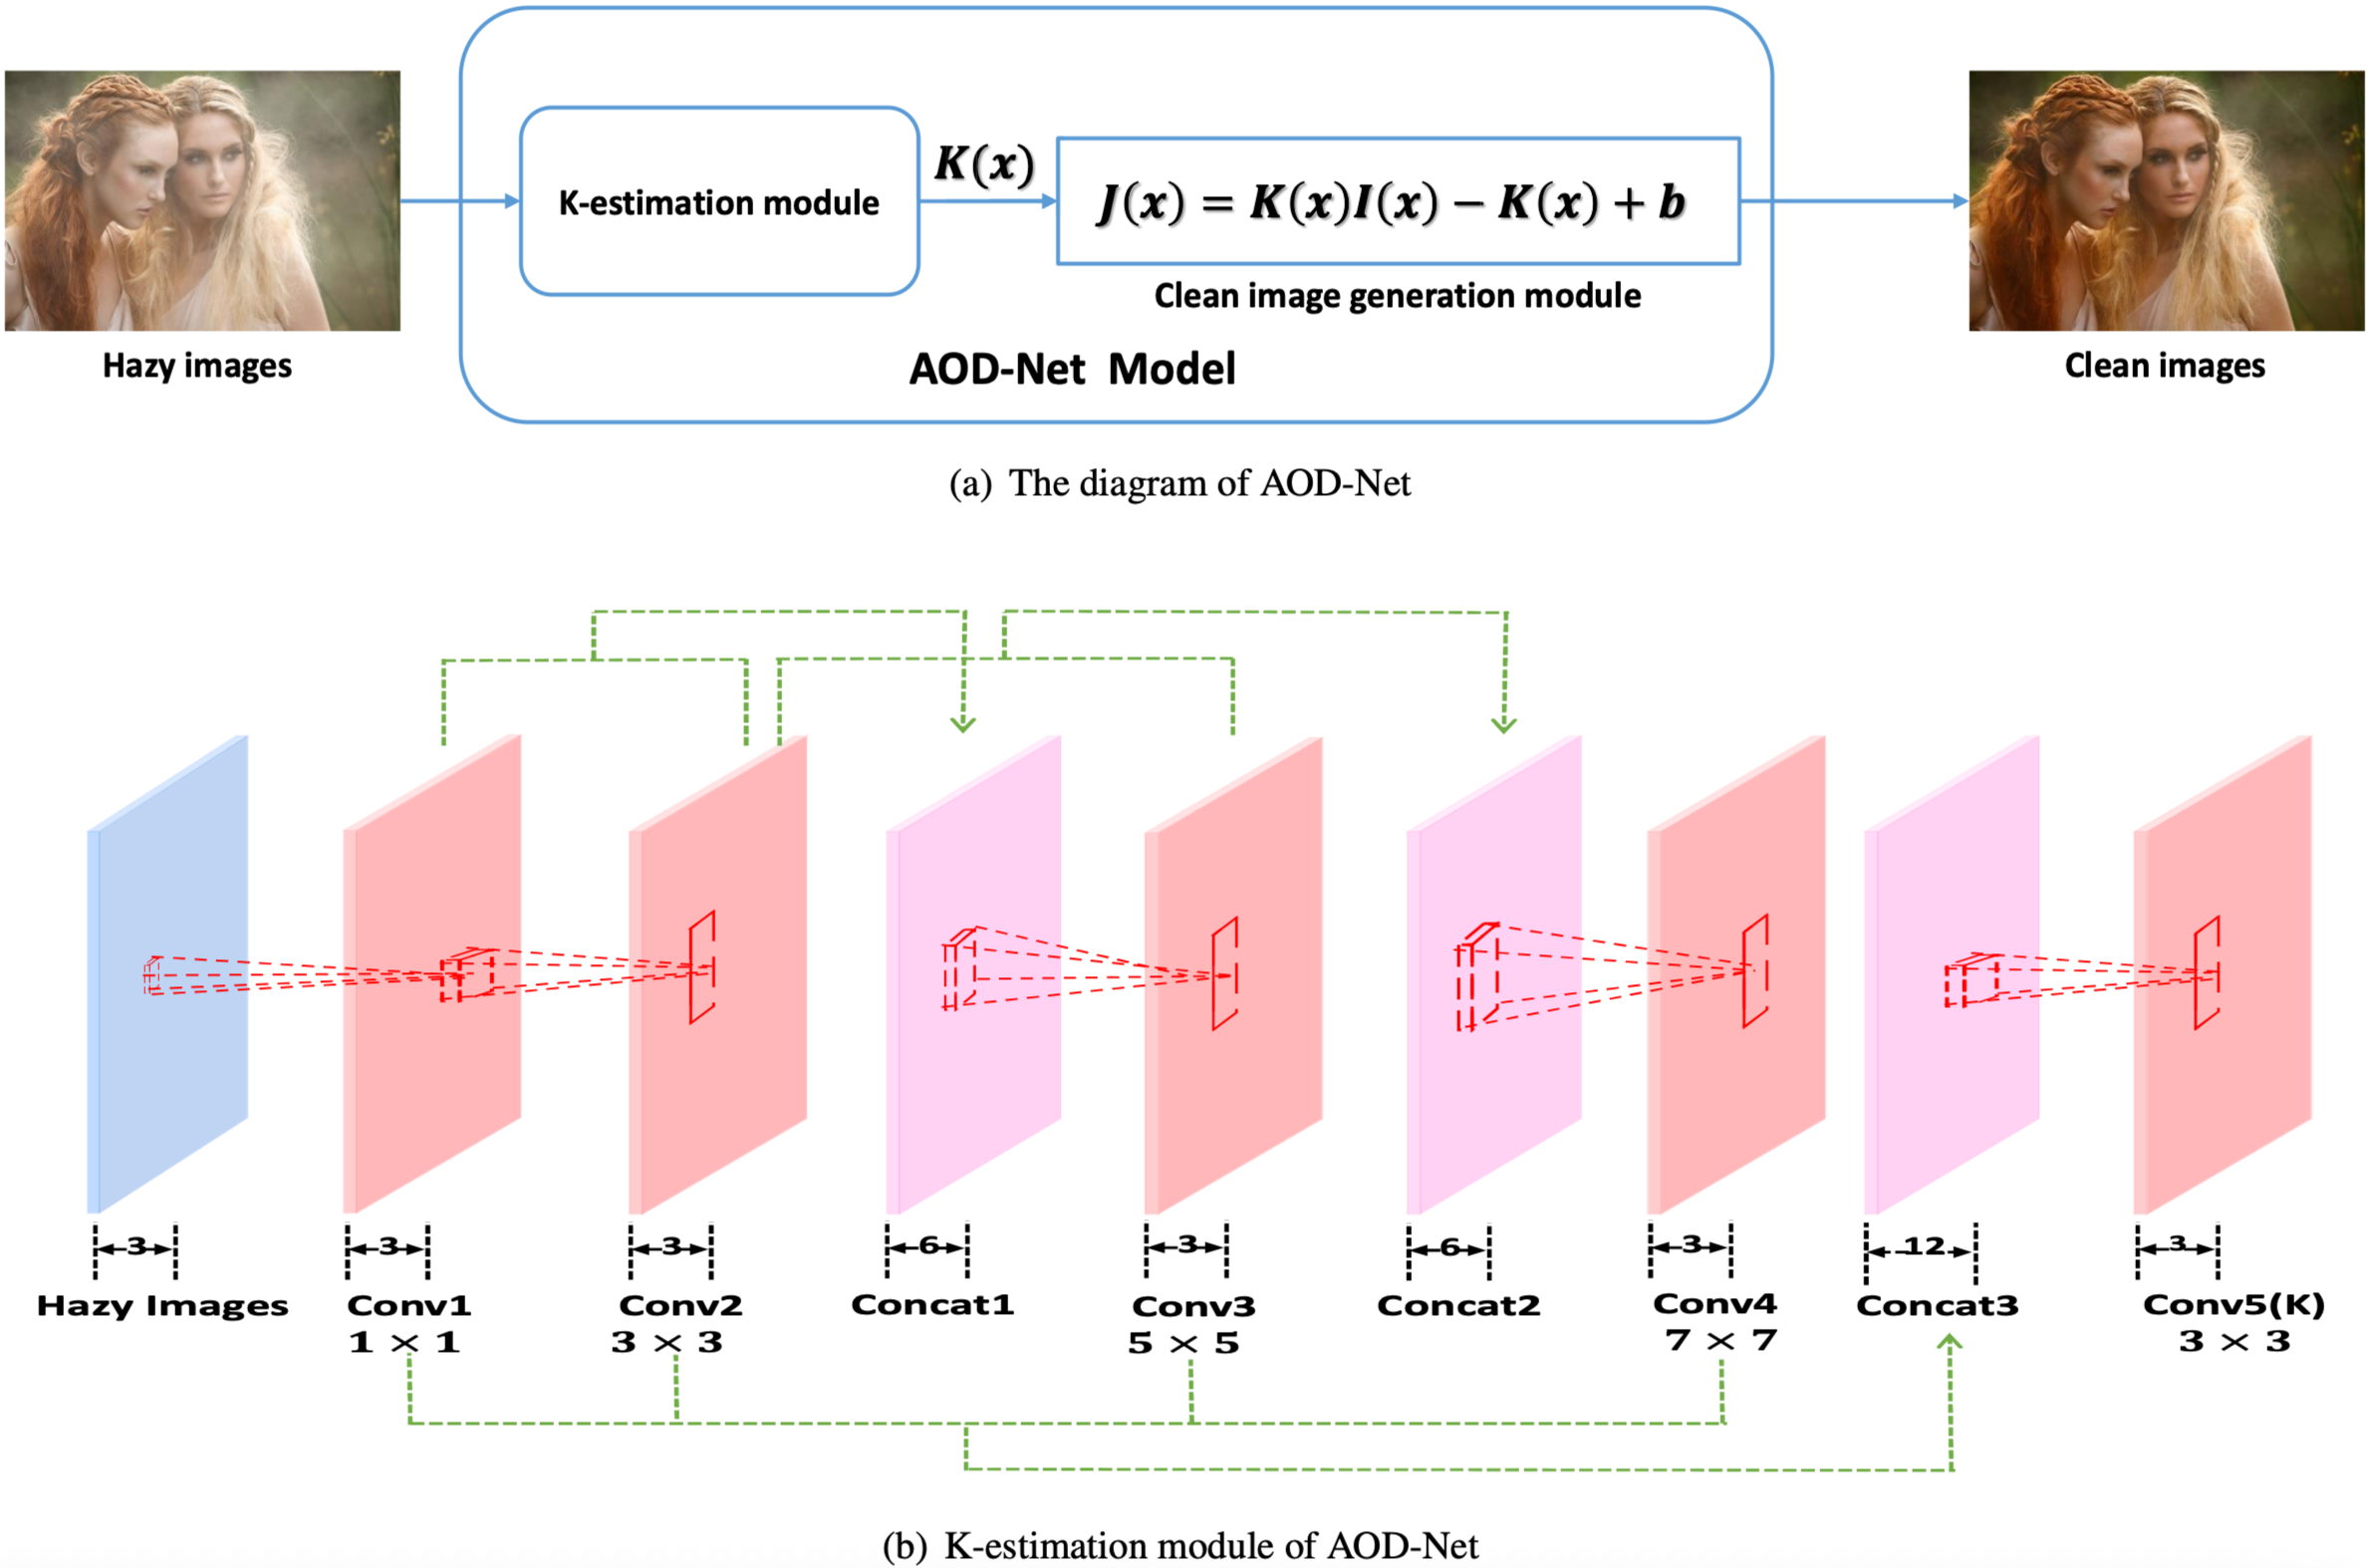
\includegraphics[width=0.8\textwidth]{../figure/aodnet.png}
    \captionsetup{font=footnotesize}
    \bicaption{AOD-Net 网络\cite{li2017aod}}{AOD-Net}
    \label{fig:aodnet}
\end{figure}

MSCNN\cite{zeng2017multi} 是另一种经典的基于卷积神经网络的端到端去雾算法。MSCNN 网络结构如图 \ref{fig:mscnn} 所示。它创新性地采用了多尺度网络结构来解决图像去雾中的细节恢复问题。MSCNN 包括两个子网络:一个全局子网络和一个局部子网络。全局子网络用于捕捉图像中的大尺度特征,如整体场景的结构和大气光照分布等;局部子网络则侧重于提取图像中的小尺度特征,如物体的边缘和纹理细节等。通过将全局和局部子网络的输出进行融合,MSCNN 能够更准确地恢复出无雾图像中的细节信息,避免了单一尺度网络可能出现的细节丢失或模糊问题。多尺度网络结构使得该算法在处理不同复杂度和不同分辨率的图像时具有更强的适应性和灵活性。例如,在处理包含精细纹理(如树叶、毛发等)的图像时,MSCNN 能够更好地保留这些细节,使去雾后的图像更加生动逼真。不过,MSCNN 的多尺度网络结构也导致其模型参数量和计算量相对较大,在实际应用中对硬件设备的计算能力有一定的要求。

\begin{figure}[ht]
    \centering
    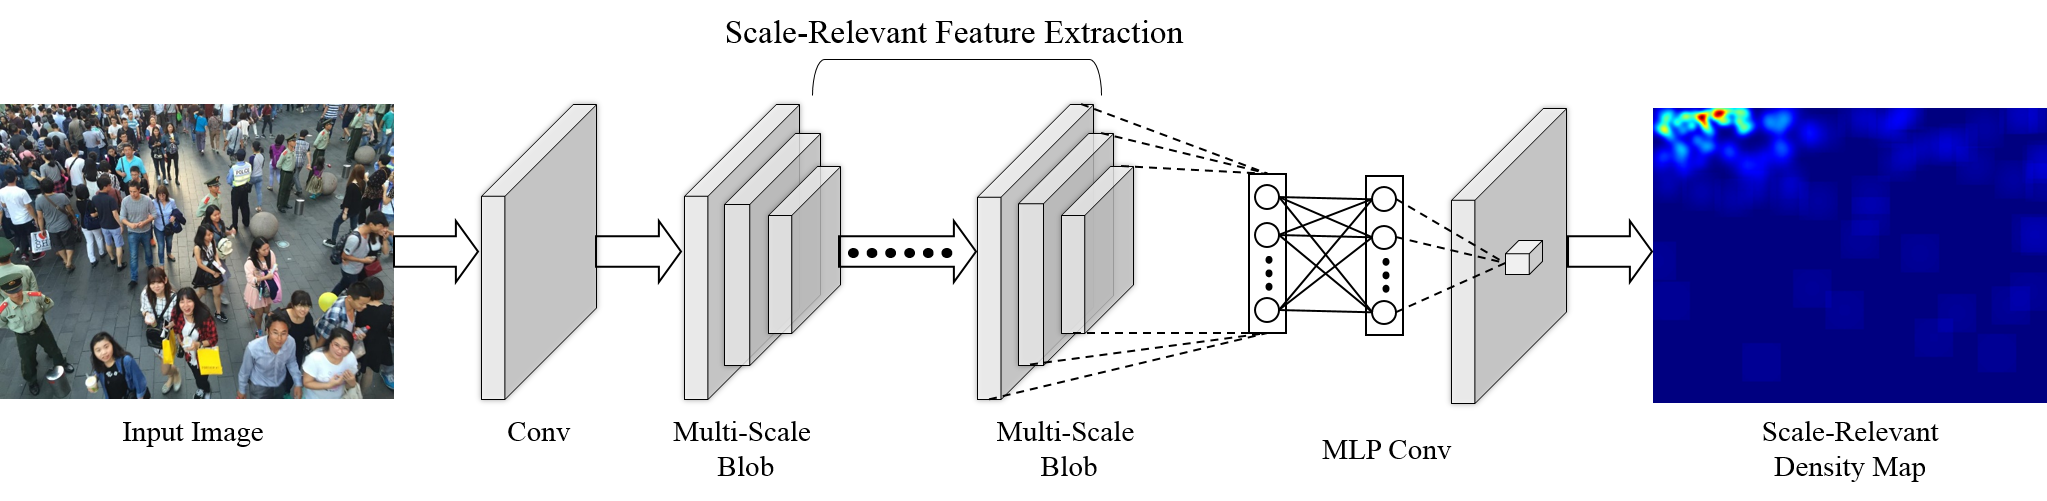
\includegraphics[width=0.9\textwidth]{../figure/mscnn.png}
    \captionsetup{font=footnotesize}
    \bicaption{MSCNN 网络\cite{zeng2017multi}}{MSCNN Net}
    \label{fig:mscnn}
\end{figure}

基于卷积神经网络的端到端去雾算法具有显著的优势。首先,它们能够自动学习图像中的复杂特征,不需要人工设计特征提取方法,大大提高了去雾算法的自动化程度和适应性。通过大量的数据训练,模型可以学习到不同类型场景、不同光照条件和不同雾浓度下的去雾模式,从而对各种雾天图像都能实现较好的去雾效果。其次,端到端的网络结构使得整个去雾过程更加简洁高效,避免了传统去雾方法中复杂的中间步骤和参数调整,减少了人工干预和计算错误的可能性。此外,随着硬件技术的发展,如图形处理器(GPU)的计算能力不断提升,这些基于卷积神经网络的端到端去雾算法能够实现较快的训练和测试速度,满足一些实时性要求较高的应用场景,如自动驾驶中的图像去雾辅助系统等。

然而,这类算法也存在一些局限性。首先,对训练数据的依赖程度较高。为了训练出性能良好的模型,需要大量的带有雾和无雾对应关系的图像数据。但在实际中,获取高质量的成对图像数据较为困难,因为很难保证在相同的场景和条件下分别拍摄到雾天和无雾的图像,并且图像的拍摄角度、光照强度等因素也可能存在差异,这会影响模型的训练效果和泛化能力。其次,模型的可解释性较差。由于卷积神经网络是复杂的黑盒模型,很难直观地理解网络内部是如何提取特征以及进行去雾映射的,这在一定程度上限制了对算法性能优化的深入研究和对特殊场景去雾效果的预测与改进。再者,一些端到端去雾算法在处理一些特殊场景或低质量的雾天图像时,可能会出现去雾效果不理想的情况,如图像出现伪影、颜色失真或细节过度增强等,这需要进一步优化网络结构和训练策略来解决。

生成对抗网络(GAN)\cite{gan}由生成器和判别器两部分组成,二者相互对抗、共同训练。生成器旨在生成逼真的无雾图像,而判别器则负责区分生成的无雾图像和真实的无雾图像。通过不断地对抗训练,生成器逐步学习到真实的图像数据分布,从而能够生成高质量的无雾图像,判别器也在这个过程中不断提升其判别能力。这种对抗训练机制使得 GAN 在图像生成和图像到图像的转换任务中展现出强大的性能,为图像去雾领域带来了新的思路和突破。

DehazeGAN\cite{raj2020single} 是较早将 GAN 引入图像去雾领域的算法之一。DehazeGAN 网络结构如图 \ref{fig:dehazegan} 所示。它通过构建生成器和判别器网络结构,利用对抗训练的思想来实现图像去雾。生成器采用编码器 - 解码器结构,编码器部分提取雾天图像的特征,解码器部分则根据提取的特征生成对应的无雾图像。判别器则是一个卷积神经网络,用于判断输入的图像是否为真实的无雾图像。在训练过程中,生成器和判别器不断更新参数,彼此竞争,使得生成器生成的无雾图像在视觉效果上更加逼真。DehazeGAN 在一定程度上提高了图像去雾的效果,能够生成较为自然的无雾图像,并且在一些简单的雾天图像场景下表现良好。然而,该算法也存在一些不足之处,例如在处理复杂场景时,生成的无雾图像可能会出现一些伪影,且对训练数据的质量和数量较为敏感,当训练数据不足或质量较差时,模型的性能会受到较大影响。

\begin{figure}[ht]
    \centering
    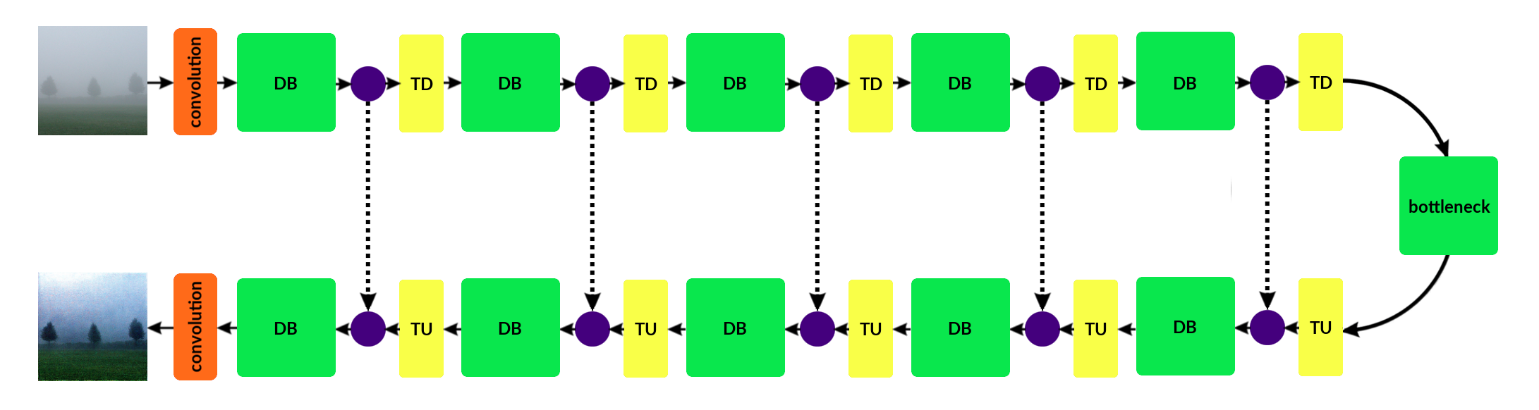
\includegraphics[width=0.8\textwidth]{../figure/dehazeGANG.png}
    \\
    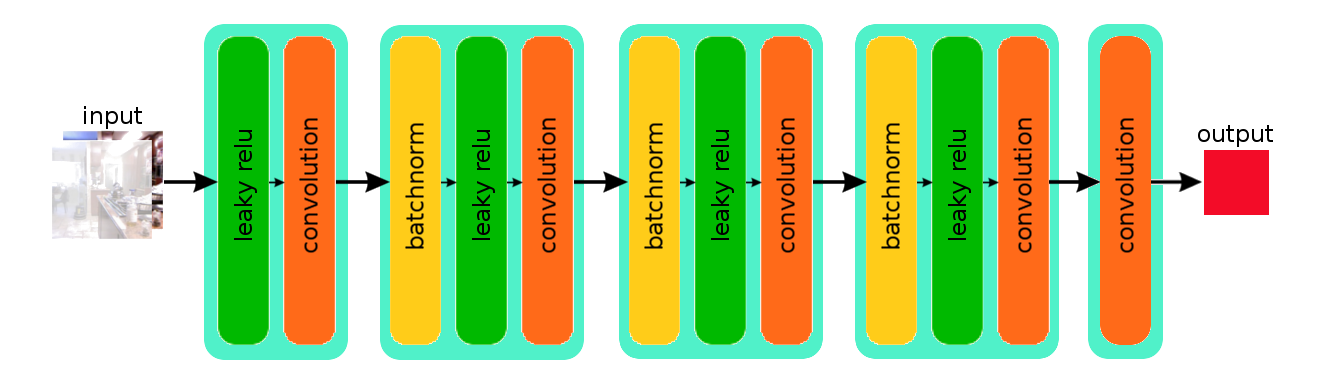
\includegraphics[width=0.8\textwidth]{../figure/dehazeGAND.png}
    \captionsetup{font=footnotesize}
    \bicaption{DehazeGAN 网络\cite{raj2020single}}{DehazeGAN Net}
    \label{fig:dehazegan}
\end{figure}

为了克服 DehazeGAN 等算法存在的问题,CycleDehazeGAN 被提出\cite{cgan}。CycleDehazeGAN 网络结构如图 \ref{fig:cycledehaze} 所示。该算法引入了循环一致性损失函数,通过构建两个生成器和两个判别器,实现从雾天图像到无雾图像以及从无雾图像到雾天图像的双向转换,并利用循环一致性约束来保证图像在转换过程中的信息完整性和一致性。具体来说,一个生成器将雾天图像转换为无雾图像,另一个生成器将无雾图像转换为雾天图像,同时两个判别器分别对转换后的无雾图像和雾天图像进行判别。循环一致性损失函数确保了经过双向转换后的图像与原始图像在内容和结构上的一致性,从而有效地避免了图像在转换过程中出现信息丢失或伪影等问题。CycleDehazeGAN 在处理复杂场景和多样化数据时具有更好的稳定性和鲁棒性,能够生成更高质量的无雾图像,并且在无监督学习环境下也能取得较好的去雾效果,扩大了其应用范围。

\begin{figure}[ht]
    \centering
    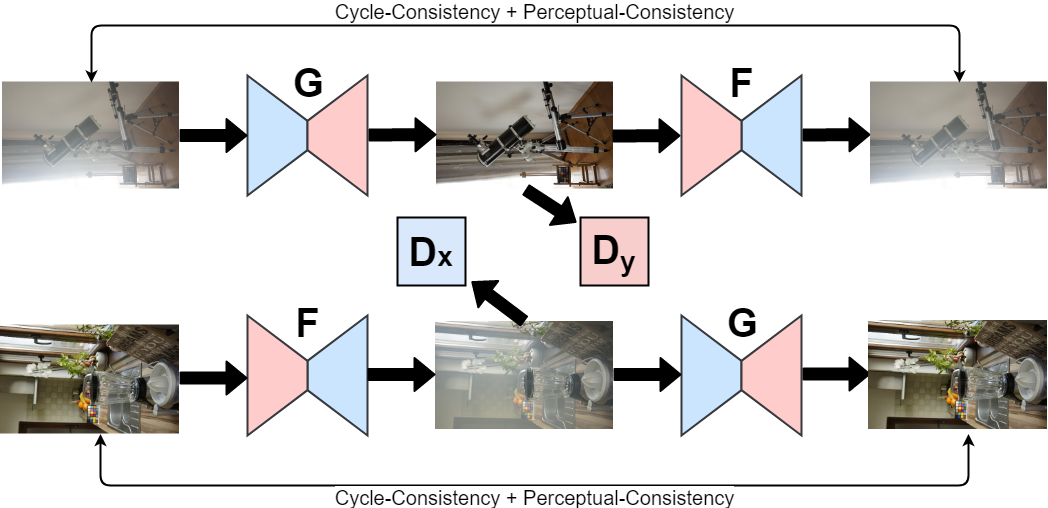
\includegraphics[width=0.7\textwidth]{../figure/Cycle-Dehaze.png}
    \captionsetup{font=footnotesize}
    \bicaption{CycleDehazeGAN 网络\cite{cgan}}{CycleDehazeGAN Net}
    \label{fig:cycledehaze}
\end{figure}

基于 GAN 的图像去雾算法具有显著的优势。首先,GAN 的对抗训练机制能够使生成器生成的无雾图像在视觉效果上更加逼真,更好地保留了图像的细节和纹理信息,避免了传统去雾方法可能出现的过度平滑或细节丢失等问题。例如,在去雾后的图像中,物体的边缘更加清晰锐利,表面的纹理更加丰富自然,这有助于提高图像的视觉质量和后续计算机视觉任务的准确性。其次,GAN 方法能够实现无监督或弱监督学习,在一定程度上缓解了获取大量成对雾天图像和无雾图像数据困难的问题,扩大了算法的应用范围和实用性,可以利用更多的未标注数据进行训练,提高了模型的泛化能力。再者,GAN 的灵活架构使得研究人员可以根据不同的需求和场景对网络结构进行定制和改进,例如引入多尺度结构、注意力机制等,以进一步提升去雾效果和适应性。


\subsection{目标检测算法的评价指标}

\subsubsection{基础指标}

准确率是指在所有被预测为正样本(即检测到目标)的结果中,实际为真阳性(True Positive)的比例。其计算公式如下:
\begin{equation}
    \label{eq:p}
    P = \frac{TP}{TP+FP}
\end{equation}

公式 \ref{eq:p} 中,$TP$(True Positive)代表正确检测到的目标数量,$FP$(False Positive)表示错误检测到的目标数量。准确率越高,表明算法在预测目标存在时的可信度越高,对虚假目标的误判越少。例如,在安防视频监控的目标检测场景中,较低的准确率可能导致大量误报,增加人工审核工作量,而高准确率的算法能有效减少此类干扰,精准定位真正可疑目标。


召回率衡量的是算法在所有真实存在的目标中,能正确检测出的比例。计算公式为:
\begin{equation}
    \label{eq:r}
    R = \frac{TP}{TP+FN}
\end{equation}

公式 \ref{eq:r} 中,$FN$(False Negative)表示未被检测到的真实目标数量。召回率反映了算法对目标的全面捕捉能力。以医学影像中的病变检测为例,过低的召回率意味着许多病变可能被遗漏,延误诊断,高召回率的算法可确保尽可能多地发现潜在病变区域,为后续的诊断分析提供更完整的信息基础。

帧率是与推理时间密切相关的指标,表示每秒能处理的图像帧数,计算公式为:
\begin{equation}
    \label{eq:fps}
    FPS = \frac{1}{Inference\ Time}
\end{equation}

公式 \ref{eq:fps} 中,$Inference\ Time$ 表示的是推理时间。推理时间是指算法对一张图像完成目标检测所需的时间,它直接决定了算法在实际应用中的实时性表现。通常以毫秒(ms)为单位,推理时间越短,算法的实时性越好。较高的帧率意味着算法能更流畅地处理视频流数据。在体育赛事直播中的目标检测应用(如运动员动作捕捉、球类追踪等),为了给观众提供实时、连贯的视觉特效和数据分析,需要算法具备较高的帧率,确保对每一帧视频都能及时准确地检测出目标物体,保证整个直播过程的流畅性和信息准确性。

\subsubsection{综合评价指标}

F1 - Score 是准确率和召回率的调和平均数,在一定程度上平衡了两者的关系,尤其在需要同时兼顾检测准确性和全面性的场景中具有重要意义。其公式为:
\begin{equation}
    \label{eq:f1}
    F1=\frac{2\cdot{P}\cdot{R}}{P+R}
\end{equation}

当准确率和召回率都较高时,F1 - Score 才能取得较大值。例如在自动驾驶场景下,对于车辆检测,既要保证将大部分车辆都检测出来(高召回率),避免遗漏引发碰撞风险;又要确保检测到的车辆信息真实可靠(高准确率),防止因虚假车辆信息导致决策失误,此时 F1 - Score 能很好地综合评估车辆检测算法的性能优劣。

AP 是评估目标检测算法的一个关键指标,尤其在多类别目标检测任务中广泛应用,计算公式为:
\begin{equation}
    \label{eq:AP}
    AP=\int_{0}^{1}p(r)\mathrm{d}r
\end{equation}

它计算的是特定类别对象在不同召回率阈值下的精确率 - 召回率曲线(PR 曲线)下的面积。AP 值越高,说明该类别目标的检测性能越好。
具体来说,首先确定一系列召回率阈值,如从 0 到 1 间隔为 0.1 的 11 个点。对于每个召回率阈值,找到对应的最大精确率,然后计算这些最大精确率的平均值即为 AP。例如在 COCO(Common Objects in Context)数据集的目标检测任务中,会对每个类别分别计算 AP,综合各类别 AP 可得到平均精度均值(Mean Average Precision, mAP),以此衡量整个目标检测模型在多类别上的整体性能,为模型的优化和选型提供关键数据支撑。

mAP 是多个类别 AP 的平均值,是对整个目标检测系统综合性能的一个全面衡量,计算公式为:
\begin{equation}
    \label{eq:mAP}
    mAP=\frac{1}{k}\textstyle \sum_{i=0}^{k}AP_i 
\end{equation}

它不仅考虑了各个类别目标的检测效果,还反映了算法在处理不同类型目标时的稳定性。比如在智能视频分析系统中,会涉及多种目标(如人、车、动物等)的检测,通过计算 mAP 可以直观地对比不同目标检测算法在同一数据集下的整体性能,从而选择更适合实际应用场景的算法模型。在实际应用中,mAP 计算方式也可能有一些变种,如在不同 IoU(Intersection over Union,交并比)阈值下的 mAP 等,以适应不同应用场景对检测精度的要求差异。


\subsubsection{基于位置和尺度的指标}

IoU 是衡量目标检测算法定位准确性的核心指标。它表示预测边界框(Predicted Bounding Box)与真实边界框(Ground Truth Bounding Box)交集面积与并集面积的比值。

\begin{equation}
    \label{eq:iou}
    IoU = \frac{Area_{pred} \cap Area_{gt}}{Area_{pred} \cup Area_{gt}}
\end{equation}

当 IoU 值大于等于某一设定阈值(如 0.5)时,认为该预测边界框准确定位到了目标;否则,预测结果不准确。IoU 值越接近 1,表明预测边界框与真实边界框越接近,目标定位越精确。在诸多目标检测竞赛和实际应用评估中,IoU 是不可或缺的评价标准,用于严格筛选出定位精准的检测算法,确保后续基于检测结果的应用(如图像分割、目标跟踪等)能建立在准确的目标位置信息基础上。

\subsection{图像去雾还原算法的评价指标}

PSNR 是衡量去雾图像与原始无雾图像之间差异的常用指标之一。它反映了图像像素值的均方误差(MSE)与最大可能像素值的平方之比,并以分贝(dB)为单位表示。PSNR 的计算公式为:
\begin{equation}
    \label{eq:psnr}
    PSNR = 10 \times \lg(\frac{MAX_I^2}{MSE})
\end{equation}

公式 \ref{eq:psnr} 中,$MAX_I$ 是图像像素的最大可能值,对于 8 位图像,通常为 255;$MSE$ 是均方误差,计算公式为:
\begin{equation}
    \label{eq:mse}
    MSE = \frac{1}{mn} \sum\nolimits_{i=0}^{m-1} \sum\nolimits_{j=0}^{n-1} [I(i,j) - K(i,j)]^2
\end{equation}

公式 \ref{eq:mse} 中,$I(i,j)$ 是去雾后的图像像素值,$K(i,j)$ 是原始无雾图像像素值,$m$ 和 $n$ 分别是图像的行数和列数。

较高的 PSNR 值意味着去雾后的图像与原始图像之间的差异较小,即去雾算法对图像的恢复效果较好。例如,当 PSNR 值达到 30 dB 以上时,通常认为去雾后的图像质量较好,与原始图像较为接近。然而,PSNR 也存在一定的局限性,因为它仅仅基于像素值的差异进行计算,可能无法完全反映图像的视觉质量,例如当去雾后的图像在整体亮度或色彩上有一定偏差,但像素值差异较小时,PSNR 可能仍然较高。


SSIM 是一种更关注图像结构信息的评价指标。图像的结构信息反映了物体的形状、纹理等特征。SSIM 通过对原始图像和去雾图像的亮度、对比度和结构三方面的相似性进行度量,综合得到一个取值范围在 -1 到 1 之间的指数。SSIM 的计算公式为:
\begin{equation}
    \label{eq:ssim}
    SSIM(x, y) = \frac{(2 \mu_x \mu_y + C_1)(2 \sigma_{xy} + C_2)}{(\mu_x^2 + \mu_y^2 + C_1)(\sigma_x^2 + \sigma_y^2 + C_2)}
\end{equation}

公式 \ref{eq:ssim} 中,$x$ 和 $y$ 分别表示原始图像和去雾图像;$\mu_x$ 和 $\mu_y$ 分别是两者的均值;$\sigma_x^2$ 和 $\sigma_y^2$ 分别是两者的方差;$\sigma_{xy}$ 是两者的协方差;$C_1$ 和 $C_2$ 是用于稳定公式的常数。

当 SSIM 值接近 1 时,说明原始图像和去雾图像在结构上具有高度相似性,即去雾算法较好地保留了图像的结构信息。与 PSNR 相比,SSIM 更能反映图像的视觉质量,因为它考虑了图像的结构特征,而不仅仅是像素值的差异。例如,在去雾后的图像中,即使某些区域的像素值略有变化,但只要物体的形状和纹理等结构信息得到较好保留,SSIM 仍可能取得较高的值。

\subsection{本章小结}

本章全面深入地探讨了目标检测与图像去雾还原的理论基础与算法进展。在目标检测领域,从双阶段算法的开创性工作R-CNN到Fast R-CNN、Faster R-CNN,再到Mask R-CNN的扩展应用,算法不断优化升级,性能逐步提升。同时,单阶段检测算法如YOLO系列的提出,实现了检测速度与精度的高效平衡,为实时性要求较高的应用场景提供了有力支持。

在图像去雾还原方面,传统算法基于物理模型和图像处理技术,为去雾研究奠定了基础。而深度学习技术的引入,如端到端的卷积神经网络、生成对抗网络等,使去雾算法在特征提取、场景适应性和图像质量提升等方面取得了显著突破。

此外,本章还系统阐述了目标检测和图像去雾还原算法的评价指标,涵盖基础指标、综合评价指标以及基于位置和尺度的指标,为客观评估算法性能提供了科学依据。总体而言,本章内容为后续研究工作奠定了坚实的理论基础,指明了目标检测与图像去雾还原领域的研究方向和应用前景。

\newpage

\section{基于YOLOv11网络改进的交通小目标检测算法\label{方法B}}

目标检测作为计算机视觉领域的核心任务之一,其算法性能直接决定了智能交通系统对车辆、行人及交通标志等目标的感知能力。在实时性与精度双重约束下,单阶段检测器YOLO\cite{yolov1, yolov2, yolov3, yolov4, yolov6, yolov7, yolov9, yolov10, yolov11}系列凭借其高效的端到端架构持续引领技术潮流。自YOLOv1被提出以来,该系列算法通过迭代式创新实现了检测精度与速度的协同优化。YOLOv3引入多尺度预测机制,YOLOv5优化训练,YOLOv8则进一步扩展至实例分割与姿态估计任务。然而,传统YOLO框架在交通小目标检测中仍面临以下挑战:(1)浅层特征图分辨率不足导致小目标细节丢失;(2)跨尺度特征融合机制对微小目标的空间信息传递效率低下;(3)复杂交通场景下背景噪声对分类置信度的干扰。

YOLOv11作为YOLO系列的最新演进版本,通过异构主干网络设计、动态特征金字塔融合及轻量化注意力机制三大核心创新,显著提升了小目标检测性能。本文基于YOLOv11网络,针对交通场景中因目标尺度小、遮挡频繁及环境干扰导致的漏检与误检问题,提出改进方案。本节将系统性阐述YOLOv11网络的核心架构设计及其在小目标检测中的理论优势。YOLOv11网络结构如图\ref{fig:YOLOv11}所示。

\subsection{YOLOv11网络结构分析}

\begin{figure}[htb]
    \centering
    \subfloat{
        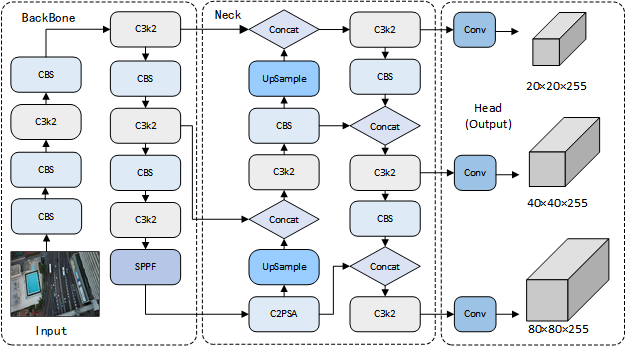
\includegraphics[width=0.8\linewidth]{../figure/yolov11.png}
    }
    \captionsetup{font=footnotesize}
    \bicaption{YOLOv11网络结构}{YOLOv11 network structure diagram.}
    \label{fig:YOLOv11}
\end{figure}

\subsubsection{主干网络}

YOLOv11 的主干网络是其整体架构的核心组成部分,其设计目标是通过改进特征提取能力来提升目标检测的精度,同时在计算效率和模型复杂度之间取得平衡。YOLOv11 的主干网络在继承了 YOLO 系列一贯的高效性和实时性特点的基础上,进一步优化了特征提取的深度和广度,以适应复杂场景下的目标检测需求。

YOLOv11 的主干网络通过多层次的特征金字塔结构(Feature Pyramid Network, FPN),能够提取不同尺度的特征,从而更好地处理不同大小的目标。这种设计特别适用于交通场景中的小目标检测,因为小目标的特征往往分布在较浅的特征层,而大目标则需要更深的特征层来捕捉。
主干网络采用了模块化的设计思路,通过堆叠多个基础模块(如卷积层、池化层和注意力模块)来构建深度网络。这种模块化设计不仅提高了网络的灵活性,还使得网络能够根据具体任务的需求进行调整。
YOLOv11 的主干网络在设计上注重参数的高效利用,通过减少冗余计算和优化网络结构,使得模型在保持高精度的同时,显著降低了参数量和计算复杂度。

YOLOv11 的主干网络基于改进的 CSPDarknet 架构,该架构通过引入跨阶段部分连接(Cross Stage Partial Connections, CSP)技术,显著提高了特征提取的效率和精度。

主干网络首先通过一个输入层接收图像数据,随后经过一系列初始卷积层(Convolutional Layers)进行特征提取。这些卷积层通常采用 $3\times3$ 或 $1\times1$ 的卷积核,用于提取图像的基本特征,如边缘、纹理和颜色信息。初始卷积层的设计旨在快速缩小特征图的尺寸,同时增加特征图的深度,为后续的特征提取奠定基础。
主干网络特征提取过程如图 \ref{fig:YOLOv11_BackBone_input} 所示。
\begin{figure}[htb]
    \centering
    \subfloat{
        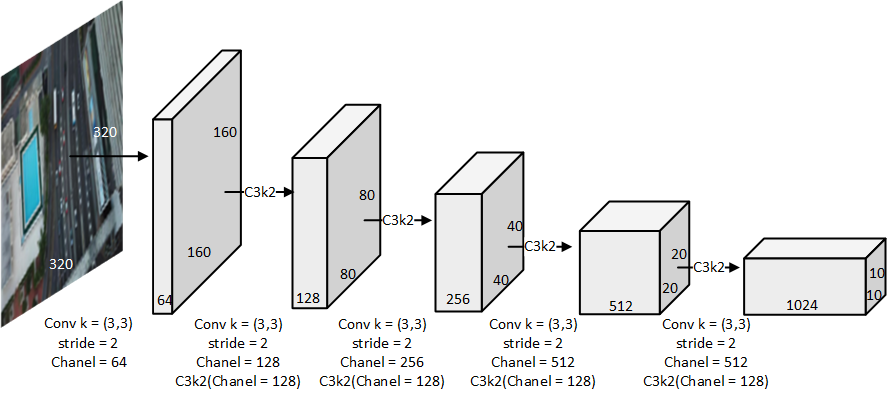
\includegraphics[width=0.8\linewidth]{../figure/yolov11_backbone_input.png}
    }
    \captionsetup{font=footnotesize}
    \bicaption{YOLOv11主干网络输入过程}{YOLOv11 BackBone network structure diagram.}
    \label{fig:YOLOv11_BackBone_input}
\end{figure}

主干网络中包含多个瓶颈模块(Bottleneck Module),这些模块通过 $1\times1$ 卷积层减少特征图的深度,随后通过 $3\times3$ 卷积层进行特征提取,最后再通过 $1\times1$ 卷积层恢复特征图的深度。这种设计在不显著增加计算量的情况下,提高了特征提取的深度和精度。
CBS 模块、BottleNeck 模块如图 \ref{fig:cbs} 、图 \ref{fig:bottleneck} 所示。
\begin{figure}[htb]
    \centering
    \subfloat{
        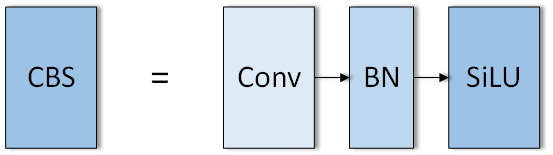
\includegraphics[width=0.5\linewidth]{../figure/cbs.png}
    }
    \captionsetup{font=footnotesize}
    \bicaption{CBS 模块}{YOLOv11 BackBone network structure diagram.}
    \label{fig:cbs}
\end{figure}

\begin{figure}[htb]
    \centering
    \subfloat{
        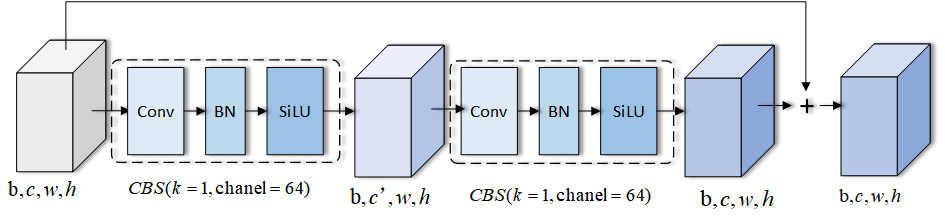
\includegraphics[width=0.9\linewidth]{../figure/bottleneck.png}
    }
    \captionsetup{font=footnotesize}
    \bicaption{BottleNeck模块}{YOLOv11 BackBone network structure diagram.}
    \label{fig:bottleneck}
\end{figure}

CSP 模块是 YOLOv11 主干网络的核心组成部分,其设计灵感来源于残差网络(ResNet)中的残差块。CSP 模块通过将特征图分为两部分,一部分直接传递到下一层,另一部分经过卷积操作后再与前一部分进行拼接,从而减少了计算量并提高了特征提取的效率。CSP 模块的引入不仅增强了网络的特征提取能力,还有效缓解了梯度消失问题,使得网络能够更深层次地学习目标的特征。
C3k2 模块、C2PSA 模块以及 PSA Block 模块如图 \ref{fig:c3k2} 、图 \ref{fig:psablock} 所示。
\begin{figure}[htb]
    \centering
    \subfloat{
        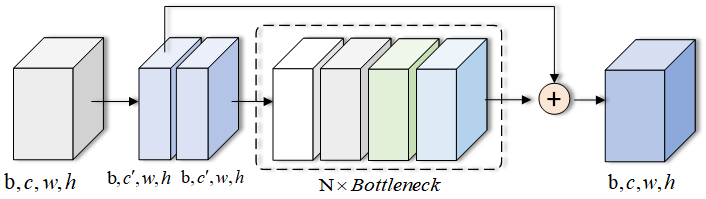
\includegraphics[width=0.8\linewidth]{../figure/c3k2.png}
    }
    \captionsetup{font=footnotesize}
    \bicaption{C3k2 模块}{YOLOv11 BackBone network structure diagram.}
    \label{fig:c3k2}
\end{figure}

\begin{figure}[htb]
    \centering
    \subfloat{
        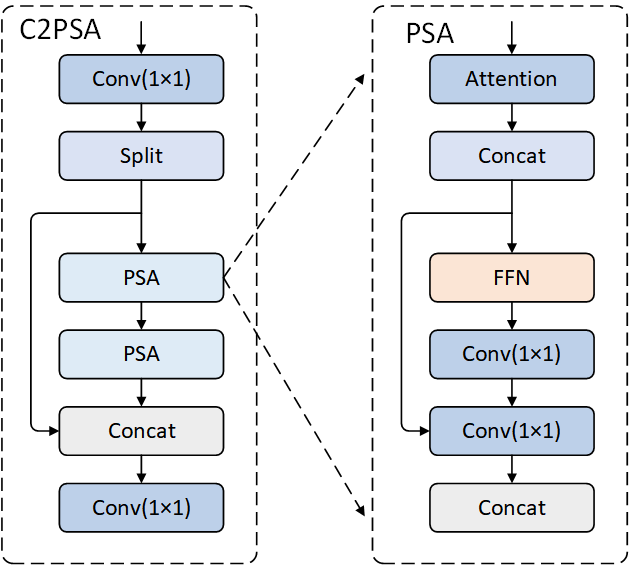
\includegraphics[width=0.6\linewidth]{../figure/pasblock.png}
    }
    \captionsetup{font=footnotesize}
    \bicaption{PSA Block模块}{YOLOv11 BackBone network structure diagram.}
    \label{fig:psablock}
\end{figure}


\subsubsection{特征融合网络}

YOLOv11 的特征融合网络是其整体架构中不可或缺的一部分,其设计目标是通过多尺度特征的融合来提升目标检测的精度和鲁棒性。特征融合网络的设计特点主要体现在以下几个方面:
多尺度特征融合:YOLOv11 的特征融合网络通过整合不同尺度的特征图,使得网络能够同时捕捉到目标的局部细节和全局上下文信息。这种设计特别适用于交通场景中的小目标检测,因为小目标的特征往往分布在较浅的特征层,而大目标则需要更深的特征层来捕捉。
自适应特征加权:YOLOv11 的特征融合网络引入了自适应特征加权机制,通过动态调整不同尺度特征图的权重,使得网络能够更加关注对检测任务更重要的特征。这种机制不仅提高了特征融合的效率,还增强了网络对复杂场景的适应能力。
高效性与实时性:特征融合网络在设计上注重计算效率和实时性,通过优化特征融合的流程和减少冗余计算,使得模型能够在资源受限的设备上高效运行。这对于交通监控系统等实时性要求较高的应用场景具有重要意义。

YOLOv11 的主干网络通过特征金字塔网络(FPN)实现了多尺度特征的融合。FPN 通过自底向上和自顶向下的路径,将不同层次的特征图进行融合,从而生成具有不同尺度的特征金字塔。这种设计使得网络能够同时捕捉到目标的局部细节和全局上下文信息,特别适用于交通场景中大小不一的目标检测。
SPPF 模块如图 \ref{fig:sppf} 所示。
\begin{figure}[htb]
    \centering
    \subfloat{
        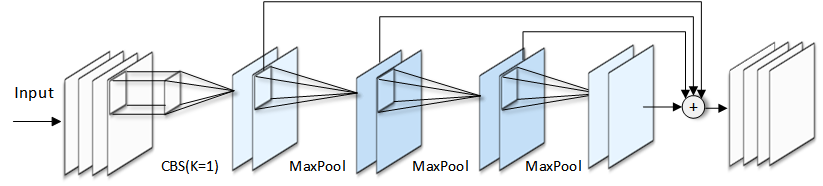
\includegraphics[width=0.85\linewidth]{../figure/sppf.png}
    }
    \captionsetup{font=footnotesize}
    \bicaption{SPPF模块}{YOLOv11 BackBone network structure diagram.}
    \label{fig:sppf}
\end{figure}

PANet 是 YOLOv11 特征融合网络的另一个重要组成部分,其通过在 FPN 的基础上引入横向连接和自底向上的增强路径,进一步优化了特征的融合过程。PANet 的设计使得特征能够在不同尺度之间更高效地流动,从而提高了特征融合的效率和检测的精度。
横向连接:PANet 在 FPN 的基础上增加了横向连接,使得不同尺度的特征图能够直接进行融合,避免了信息的丢失。
自底向上增强路径:PANet 通过自底向上的增强路径,将浅层特征的细节信息传递到深层特征中,从而进一步增强了特征的表达能力。
PANet 网络模型结构如图 \ref{fig:panet} 所示。
\begin{figure}[htb]
    \centering
    \subfloat{
    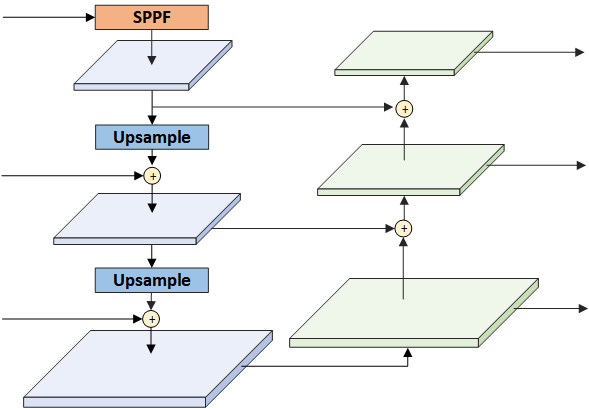
\includegraphics[width=0.6\textwidth]{../figure/panet.png}
    }
    \captionsetup{font=footnotesize}
    \bicaption{PANet网络}{YOLOv11 BackBone network structure diagram.}
    \label{fig:panet}
\end{figure}

YOLOv11 的特征融合网络通过特征融合模块将不同尺度的特征图进行融合,生成具有更高表达能力的特征图。特征融合模块通常采用逐元素加法或拼接操作,结合不同尺度的特征信息,从而提高检测的精度。

\subsection{优化的YOLO网络}

作为一个轻量级目标探测器,YOLOv11以其高效的性能和简单的架构而闻名。 然而,在处理小目标时,YOLOv11存在以下主要问题:(a)特征表征能力不足:YOLOv11采用的特征提取网络没有充分考虑小目标的特征表征,导致小目标的定位精度和检测精度降低。(b)规模感知不足:原始的YOLOv11模型缺乏多尺度目标检测的有效策略,对小目标规模变化的适应性差,容易导致遗漏或误认检查。 这些问题限制了YOLOv11在小目标检测场景中的应用效果。 

为了解决这些问题,本文提出了一系列基于现有方法的改进措施,包括多尺度融合模块SPPC模块、轻量级卷积模块DBSS模块和更高效的损失函数NWD损失函数,以提高检测性能,同时保持模型的轻量级。
用YOLOv11的SPPF模块替换改进的SPPC模块,以提高模型对小目标的检测性能。
使用DBS模块替换YOLOv11中的CBS,并使用DC3k2替换C3k2模块,这可以大大减少计算量,同时保持小目标的检测性能。
使用DBSS注意模块插入到第3层和第5层中,以提高模型对小目标的检测性能 
新方法的模型是EX-YOLO,如图\ref{fig:ex_yolo_detail}所示。

\begin{figure}[htbp]
    \centering
    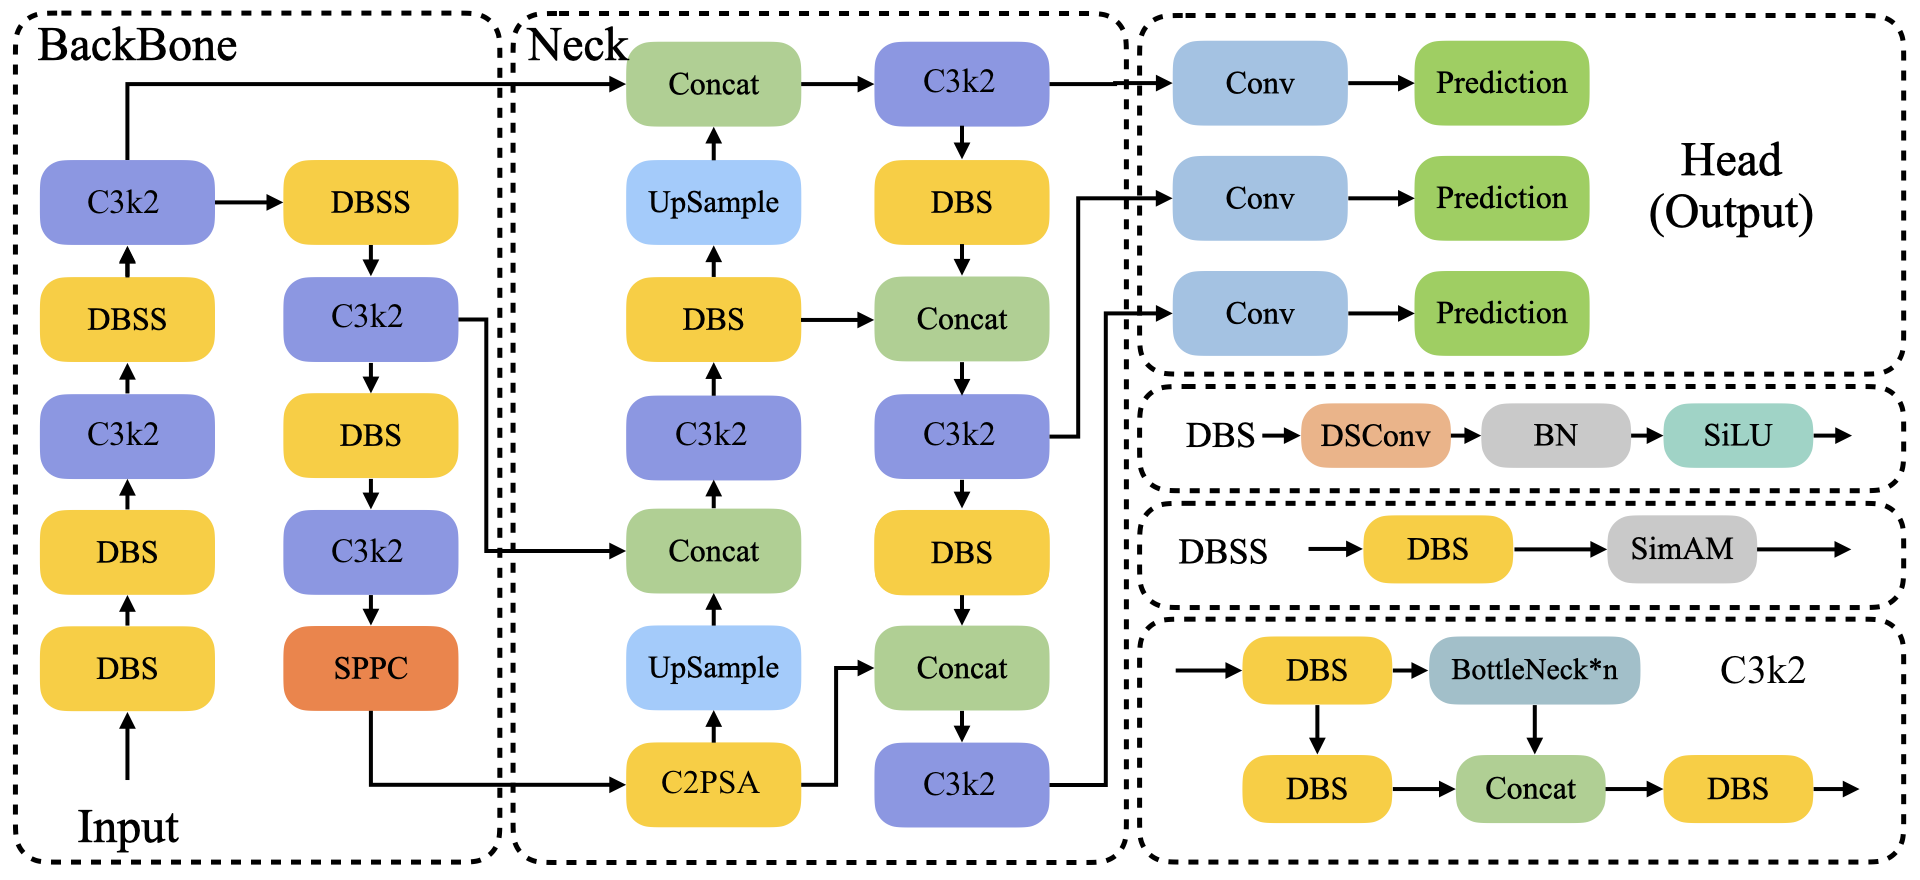
\includegraphics[width=0.9\textwidth]{../figure/ex_yolo_detail.png}
    \captionsetup{font=footnotesize}
    \bicaption{EX-YOLO 网络模型结构}{Some descriptions of the pictures in question.}
    \label{fig:ex_yolo_detail}
\end{figure}


\subsubsection{改进的特征融合模块}

在无人机的小目标检测任务中,传统目标检测算法经常面临特征提取能力不足的问题,特别是在处理中小型目标时,特征图分辨率低,导致关键信息丢失。 
作为一种先进的目标检测算法,尽管YOLOv11在速度和准确性方面表现良好,但在小目标检测任务方面仍有改进的余地。 
为了进一步增强中小型目标模型的特征提取能力,我们提出了SPPC模块。
SPPC模块结合了SPPF模块的多尺度特征提取能力和CAM的特征增强能力,从而提高了中小型目标模型的特征捕获能力,从而提高了mAP。

SPPC模块的结构如图\ref{fig:sppc}所示。
模块的输入特征图首先通过$1\times1$卷积层(cv1)按通道数进行压缩,然后是多个最大池操作(MaxPool),在池过程中将功能增强插入CAM模块中。
最后,所有特征图都通过$1\times1$卷积层(cv2)融合,以输出特征图。

CAM模块的核心设计是通过多尺度卷积运算提取特征,并通过融合增强特征表达。 CAM模块的结构如图\ref{fig:cam}所示,具体公式如下:
\begin{subnumcases}{\label{eq:cam1}}
% \begin{aligned}
    x_1 = Conv(x, kernel=3, dilation=1) \\
    x_2 = Conv(x, kernel=3, dilation=3) \\
    x_3 = Conv(x, kernel=3, dilation=5) 
% \end{aligned}
\end{subnumcases}
公式 \ref{eq:cam1} 中,$x_1$、$x_2$和$x_3$分别表示不同扩展率卷积的输出。
然后,通过$1\times1$卷积进行特征融合:
\begin{subnumcases}{}
    \label{eq:cam2}
% \begin{aligned}
    f_1 = Conv(x_1, kernel=1) \\
    f_2 = Conv(x_2, kernel=1) \\
    f_3 = Conv(x_3, kernel=1)
% \end{aligned}
\end{subnumcases}

最后,CAM模块的输出是:
\begin{equation}
    \label{eq:cam3}
    y = Concat(f_1, f_2, f_3)
\end{equation}

\begin{figure}[htbp]
    \centering
    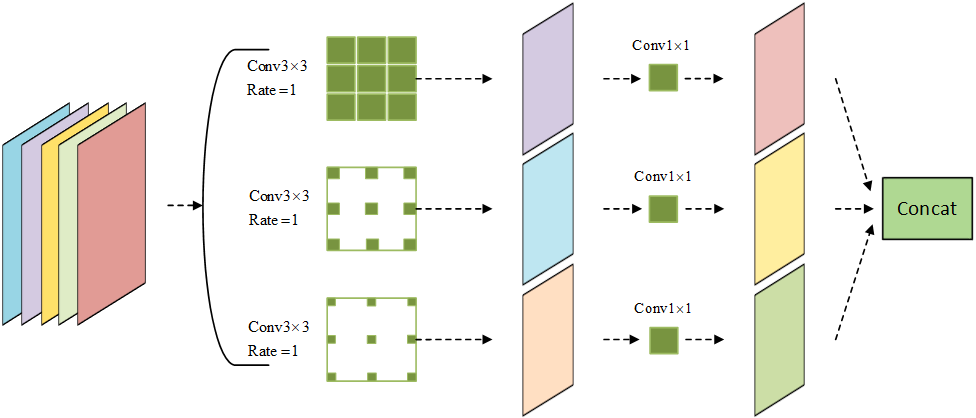
\includegraphics[width=0.7\textwidth]{../figure/CAM.png}
    \captionsetup{font=footnotesize}
    \bicaption{CAM 模块}{Some descriptions of the pictures in question.}
    \label{fig:cam}
\end{figure}

\begin{figure}[htbp]
    \centering
    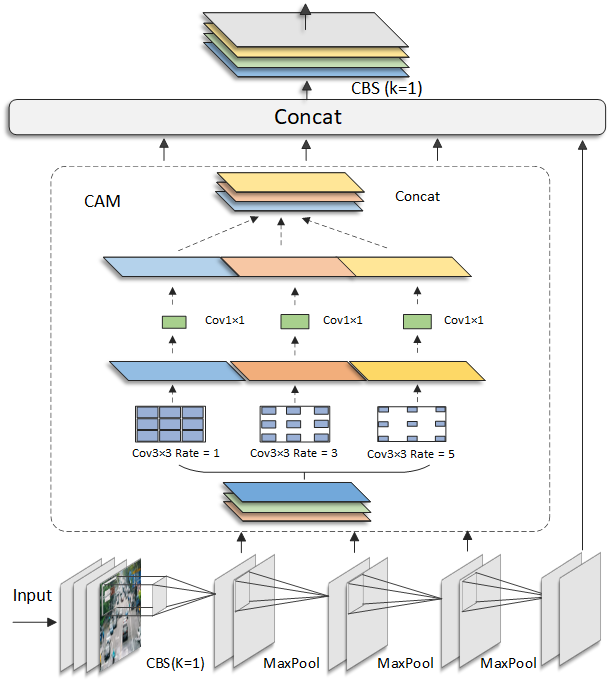
\includegraphics[width=0.6\textwidth]{../figure/SPPC.png}
    \captionsetup{font=footnotesize}
    \bicaption{SPPC 模块}{Some descriptions of the pictures in question.}
    \label{fig:sppc}
\end{figure}

SPPC模块的核心是将CAM模块嵌入到SPPF的池化过程中。 具体实现如下:(a)输入特征图$x$首先通过$1\times1$卷积层(cv1)和输出特征图$y_0$进行压缩。 在$y_0$上执行三个最大池操作(m),每次池后的功能图分别记录为$y_1$、$y_2$、$y_3$:
\begin{subnumcases}{}
% \begin{aligned}
    y_0 = cv_1(x) \\
    y_1 = m(y_0) \\
    y_2 = m(y_1) \\
    y_3 = m(y_2) 
% \end{aligned}
    % y_0 = cv_1(x), y_1 = m(y_0), y_2 = m(y_1), y_3 = m(y_2)
\end{subnumcases}

(b)将CAM模块插入$y_0$、$y_1$、$y_2$,以增强特征表达能力:
\begin{subnumcases}{}
% \begin{aligned}
    y_0' = CAM(y_0) \\
    y_1' = CAM(y_1) \\
    y_2' = CAM(y_2)  
% \end{aligned}
% y_0' = CAM(y_0), y_1' = CAM(y_1), y_2' = CAM(y_2)
\end{subnumcases}

(c)将增强功能图$y_0'$、$y_1'$、$y_2'$与功能图$y_3$进行匹配:
\begin{equation}
    y_{concat} = Concat(y_0', y_1', y_2', y_3)
\end{equation}

(d)最后,通过$1\times1$卷积层(cv2)进行通道融合,并输出最终特征图$y$:
\begin{equation}
    y = cv2(y_{concat})
\end{equation}

SPPC模块可以通过结合SPPF和CAM模块来有效地提取多尺度功能。
SPPF模块通过最大池操作捕获不同尺度的上下文信息,而CAM模块通过多尺度卷积和通道融合进一步增强了特征表达能力。
这种设计使模型能够更好地适应中小型目标的特征提取需求。

\subsubsection{轻量化的卷积模块}

YOLOv11的特征提取网络依靠标准卷积操作(nn.Conv2d)来提取图像的特征信息。 
尽管YOLOv11在目标检测任务中表现出色,但其基于标准卷积层的特征提取网络在计算资源有限的设备上的计算复杂性和资源消耗方面仍存在一些缺点。 
为了降低YOLOv11的计算复杂性和模型参数,并将精度损失最小化,本文介绍了一个轻量级卷积单元——深度可分离卷积(DSC)。 

DSC模块的核心结构如图\ref{fig:DSC}所示。该模块主要由深度卷积、点卷积和动态重量调节模块组成。

(a)深度卷积是每个输入通道上的单独卷积操作。 卷积内核的数量等于输入通道的数量,每个卷积内核只作用于一个通道。 这种方法大大减少了卷积运算的计算量。 深度卷积的数学表达式是:
\begin{equation}
    \label{eq:dsc1}
    O_i = \sum\limits_{k\in{K}}{I_i\otimes{W_{k,i}}}
\end{equation}

公式 \ref{eq:dsc1} 中,$O_i$表示第$i$个输出通道,$I_i$表示第$i$个输入通道,$W_{k,i}$表示作用于$i$通道的卷积内核,$K$表示卷积内核的大小,$\otimes$表示卷积操作。

(b)点卷积是一种$1\times1$卷积操作,用于将深度卷积的输出通道数调整到目标通道数。 点卷积的数学表达式是:
\begin{equation}
    \label{eq:dsc2}
    O = \sum\limits_{i=1}^{C_{in}}I_i\otimes{W_i}
\end{equation}

公式 \ref{eq:dsc2} 中,$O$表示输出通道,$C_{in}$表示输入通道数,$I_i$表示第$i$个输入通道,$W_i$表示点卷积的权重。

(c)为了进一步减少计算量,DSC模块引入了动态权重调整机制。 通过将输入通道划分为多个块,每个块使用共享权重参数$\alpha$来动态调整卷积内核的权重。 具体实现如代码所示。 $\alpha$参数根据块数和通道数展开,并乘以卷积内核权重来生成最终卷积权重。 动态重量调整模块的数学表达式是:
\begin{equation}
    \label{eq:dsc3}
    W_{res} = \alpha\odot{W_{net}}
\end{equation}

公式 \ref{eq:dsc3} 中,$W_{res}$表示调整后的卷积权重,$\alpha$表示动态权重参数,$W_{net}$表示原始卷积权重,$\odot$表示元素乘法。

标准卷积的核心结构如图\ref{fig:nnConv}所示。标准卷积的计算可以通过以下公式来计算:
\begin{equation}
    \label{eq:conv}
    F_{conv} = {C_{in}}\times{C_{out}}\times{K^2}\times{H}\times{W}
\end{equation}

公式 \ref{eq:conv} 中,$C_{in}$表示输入通道数,$C_{out}$表示输出通道数,$K$表示卷积内核的大小,$H$和$W$表示输入特征图的高度和宽度。 

DSC模块的计算体积由两部分组成,深度卷积和点卷积:
\begin{equation}
\begin{aligned}
    F_{depth} &= {C_{in}}\times{K^2}\times{H}\times{W} \\
\end{aligned} 
\label{eq:dsconv_depth}
\end{equation}

\begin{equation}
\begin{aligned}
    F_{point} &= {C_{in}}\times{C_{out}}\times{H}\times{W} \\
\end{aligned} 
\label{eq:dsconv_point}
\end{equation}

\begin{equation}
\begin{aligned}
    F_{DSC} &= F_{depth} + F_{point} \\
            &= {C_{in}}\times\left({K^2+C_{out}}\right)\times{H}\times{W}
\end{aligned} 
\label{eq:dsconv}
\end{equation}

通过比较方程\ref{eq:conv}和方程\ref{eq:dsconv},可以发现DSC模块的计算量显著降低。

\begin{figure}[htbp]
    \centering
    \subfloat {
        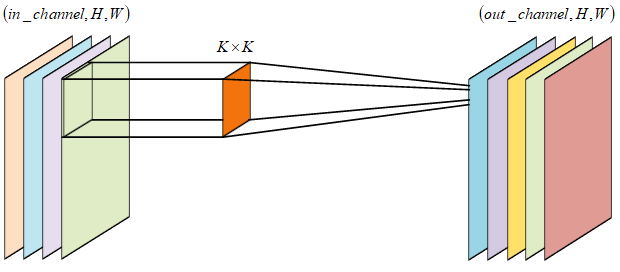
\includegraphics[width=0.7\textwidth]{../figure/nnConv.png}
    }
    \captionsetup{font=footnotesize}
    \bicaption{标准卷积模块}{Some descriptions of the pictures in question.}
    \label{fig:nnConv}
\end{figure}

\begin{figure}[htbp]
    \centering
    \subfloat {
        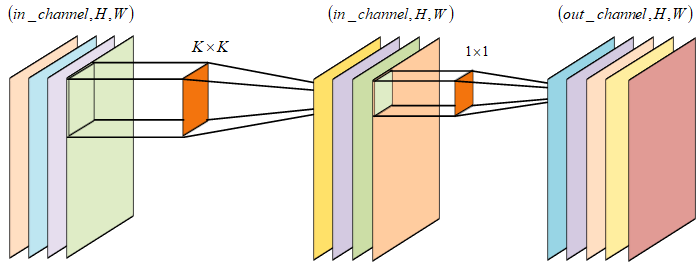
\includegraphics[width=0.7\textwidth]{../figure/DSC.png}
    } 
    % \caption{Compared nn.Conv Module with DSC Module}
    \captionsetup{font=footnotesize}
    \bicaption{DSC卷积模块}{Some descriptions of the pictures in question.}
    \label{fig:DSC}
\end{figure}

SimAM(Simple Attention Module)是一个简单且无参数的注意力模块\cite{simam}。 
SimAM通过推断特征图的3D注意力权重并优化能量函数来找出每个神经元的重要性,从而提高了各种视觉任务的性能。
SimAM通过计算特征图中每个位置的激活值与整体特征之间的相似性来动态调整每个位置的特征权重。
与传统的注意力机制相比,SimAM不依赖额外的卷积层或池操作,计算复杂性低,并且易于集成到现有的网络架构中。

SimAM的实现基于简单的数学运算,设输入特征图$x\in{R^{{B}\times{C}\times{H}\times{W}}}$,其中$B$、$C$、$H$和$W$分别表示批次数、通道数、高度和宽度。其核心公式如下:

(a)计算每个通道特征图的空间维度的平均值:
\begin{equation}
    \label{eq:simam1}
    \mu_c = \frac{1}{{H}\times{W}}\sum\limits_{i=1}^{H}\sum\limits_{j=1}^{W}x_{c,i,j}
\end{equation}

公式 \ref{eq:simam1} 中,$\mu_c$表示$c$通道的平均值。

(b)计算每个位置的激活值与通道平均值之间的相似性:
\begin{equation}
    \label{eq:simam2}
    y_{c,i,j} = \frac{(x_{c,i,j}-\mu_c)^2}{4\left(\sum_{k=1}^{H}\sum_{l=1}^{W}(x_{c,i,j}-\mu_c)^2/n+\lambda \right)}+0.5
\end{equation}

公式 \ref{eq:simam2} 中,$n={H}\times{W}-1$,$\lambda$是一个非常小的正则化常数,用于避免分母为$0$。

(c)使用Sigmoid激活函数将相似性归一化,并将归一化相似性作为输入特征图的权重应用。
\begin{equation}
    \label{eq:simam3}
    output_{c,i,j} = x_{c,i,j} \cdot \sigma(y_{c,i,j})
\end{equation}

DBSS模块连接DSC卷积单元和SimAM注意模块,以实现轻量级卷积计算和集成SimAM注意模块的轻量级模块。

\begin{figure}[htbp]
    \centering
    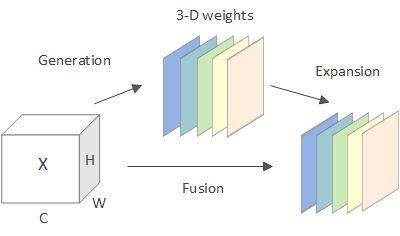
\includegraphics[width=0.6\textwidth]{../figure/SimAM.png}
    \captionsetup{font=footnotesize}
    \bicaption{SamAM 模块}{Some descriptions of the pictures in question.}
    \label{fig:SimAM}
\end{figure}

\subsubsection{更高效的损失函数}

在无人机的目标检测任务中,目标通常具有体积小、特征不显眼、背景复杂等特点,这对目标检测算法提出了更高的要求。 在处理小目标时,传统的IoU损失函数有一定的局限性。
IoU损失函数只考虑预测框和真实框之间的重叠区域。 对于小目标,预测框和真实框之间的小偏差可能会导致大的定位误差,而IoU损失函数对这些偏差不太敏感。

为了进一步提高小目标的检测性能,我们引入了NWD框损耗函数,并将其与DIoU箱损耗功能相结合。
NWD损失函数可以通过计算预测框和真实框之间的空间和规模差异来更准确地评估预测框和真实框之间的相似性,从而提高模型捕捉小目标的能力。

DIoU损失函数基于IoU损失函数的改进版本,其核心的想法是通过引入预测框和真实框中心点之间的距离来提高损失函数对空间位置的敏感性。
具体定义如下:
\begin{equation}
    \label{eq:diou}
    L_{DIoU} = 1 - \frac{A\cap{B}}{A\cup{B}} + \frac{\rho^2(c_p, c_g)}{c^2}
\end{equation}
公式 \ref{eq:diou} 中,$A\cap{B}$表示预测框和真实框的交集面积,$A\cup{B}$表示预测框和真实框的并集面积,$\rho^2(c_p, c_g)$表示预测框的中心点$c_p$和真实框的中心点$c_g$之间的欧几里得举例,$c$表示可以覆盖预测框和真实框最小闭合的对角线长度。

NWD框损失函数是通过计算预测框和真实框之间的空间和规模差异来评估的。 两者之间的相似性。
具体定义如下:
给定预测框$\mathbf{p}$和地面真理边界框$\mathbf{g}$,其中心坐标是$\mathbf{c}_p = (x_p, y_p)$和$\mathbf{c}_g = (x_g, y_g)$,宽度和高度分别为$(w_p, h_p)$和$(w_g, h_g)$。 NWD损失函数的定义是:
\begin{equation}
    L_{NWD} = \exp\left(-\frac{\sqrt{D_W}}{c}\right)
    \label{eq:nwd}
\end{equation}

公式 \eqref{eq:nwd} 中,Wasserstein距离$D_W$是:
\begin{equation}
    D_W = (\Delta x)^2 + (\Delta y)^2 + \frac{(w_p - w_g)^2 + (h_p - h_g)^2}{4} + \epsilon
    \label{eq:dw}
\end{equation}

公式 \eqref{eq:dw} 中,$\Delta x = x_p - x_g$,$\Delta y = y_p - y_g$,$\epsilon$是一个非常小的常数,以避免除法错误,$c$是用于调整距离变焦的常数。以DIoU损失函数和NWD盒子损失函数之和作为YOLOv11的盒子损失函数:
\begin{equation}
    L_{box\_loss} = \frac{L_{DIoU}+L_{NWD}}{2}
\end{equation}

通过将DIoU损失函数和NWD损失函数相加来取平均值,我们可以进一步提高模型对小目标的检测能力,同时保持大多数目标的DIoU损失函数的检测性能。
这种组合可以充分利用两种损失函数的优势,从而提高模型的整体检测性能。


\subsection{交通目标检测实验结果和分析}

新算法在TT100K数据集\cite{tt100k}和VisDrone数据集\cite{vd}上进行训练和测试,以改进每个阶段,并与YOLOv11s\cite{yolov11}进行比较。
为了在不降低其他比例目标的精度的情况下通过算法验证不同尺寸目标的检测精度,对TT100K和VisDrone的数据集进行了比较实验。
最后,在不同场景中选择复杂的场景图片,并将拟议算法的检测效果与实际场景中的YOLOv11s、YOLOv10s\cite{yolov10}和YOLOv9s\cite{yolov9}算法进行比较。

\subsubsection{数据集}

在目标检测领域,特别是对无人机小目标检测任务的研究,选择适当的数据集对于验证算法的性能至关重要。
这个实验采用了两个数据集,TT100K和VisDrone。
为了评估改进的YOLOv11算法,小目标检查测量任务的性能提供了强大的支持。

TT00K数据集由中国清华大学和腾讯团队收集。
数据集由无人机获得,是交通标志的目标识别数据集;它是在不同的场景、天气和光线下收集的,因此在复杂的环境中有许多小目标。
数据集还提供了一些属性,如场景可见性、对象类和遮挡。
图\ref{fig:tt100k_figure}显示了TT100K数据集中的一些数据。
从图\ref{fig:tt100k_figure}中可以看出,TT100K数据集中的小目标数量很小,分布不均匀,分布不在中心,并且有许多目标类别。

\begin{figure}[htbp]
    \centering
    \subfloat {
    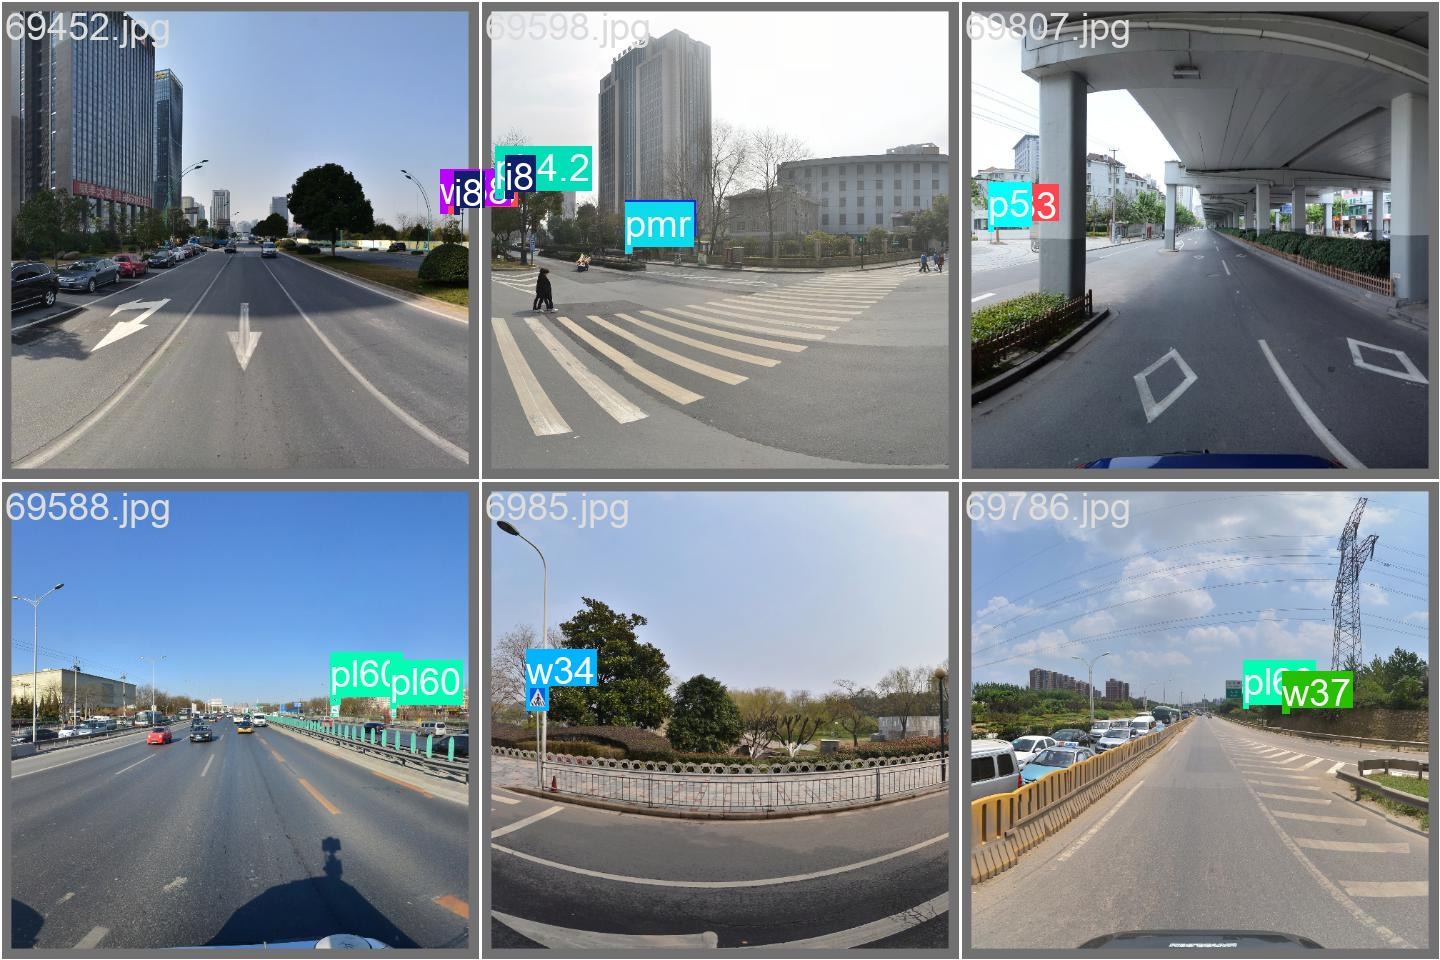
\includegraphics[width=0.8\textwidth]{../figure/TT100K.png}
    }
    \captionsetup{font=footnotesize}
    \bicaption{TT100K 数据集}{Some descriptions of the pictures in question.}
    \label{fig:tt100k_figure}
\end{figure}

VisDrone数据集是天津大学机器学习和数据挖掘实验室AISKYEYE团队创建的大规模基准数据集,专为无人机图像和视频分析中的各种计算机视觉任务而设计。
它包含288个视频剪辑、261,908帧图像和10,209个静态图像,涵盖了不同城市、环境、物体和密度的场景,并在各种天气和照明条件下收集。
图\ref{fig:vd_figure}显示了VisDrone数据集中的一些数据。
从图\ref{fig:vd_figure}中可以观察到,VisDrone数据集有大量的小目标和很少的目标类别。

\begin{figure}[htbp]
    \centering
    \subfloat {
    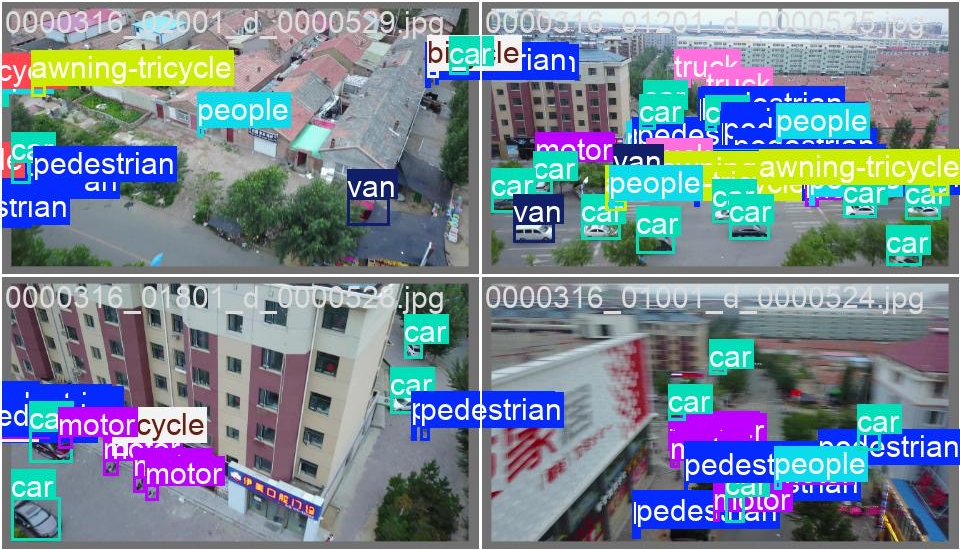
\includegraphics[width=0.8\textwidth]{../figure/VisDrone.png}
    }
    \captionsetup{font=footnotesize}
    \bicaption{VisDrone 数据集}{Some descriptions of the pictures in question.}
    \label{fig:vd_figure}
\end{figure}

虽然TT100K和VisDrone数据集不是直接基于无人机视角,但它们包含的目标类型与无人机在实际应用中需要识别的目标高度一致。
交通标志是交通检查、智能交通和其他领域中无人机的重要识别对象,而人、自行车、摩托车和汽车是安全监控、城市交通管理和其他场景中无人机的关键检测目标。
通过对这些数据集进行实验,可以间接评估改进的YOLOv11算法在无人驾驶飞行器小型目标检测任务中的潜力和优势。
与此同时,这些数据集的复杂场景和多样化的样本也为算法的泛化能力和鲁棒性测试提供了良好的基础,这有利于在不同情况下发现算法的优缺点,并为进一步优化算法以满足无人机的实际应用需求提供了重要的参考。

\subsubsection{实验环境}

本文中用于实验的系统、系统硬件设施和软件平台如表\ref{tab:environment}所示。
\begin{table}[htbp]
    \centering
    \captionsetup{font=footnotesize}
    \bicaption{实验环境设置}{Symbol cross-reference table}
    \label{tab:environment}
    \begin{tabular}{>{\centering\arraybackslash}p{0.4\textwidth}>{\centering\arraybackslash}p{0.4\textwidth}}
        \toprule
        List              & Version            \\ 
        \midrule
        Operating System  & Ubuntu 22          \\
        Memory            & 64G RAM            \\
        CPU               & Intel i9-13900K    \\
        GPU               & NVIDIA GTX4090 GPU \\
        Cuda              & cu121              \\
        Python            & 3.11               \\
        \bottomrule
    \end{tabular}
\end{table}

\subsubsection{实验结果和分析}

在这项研究中,我们通过比较实验评估了EX-YOLO模型(our)在2个不同数据集中,包括TT100K和VisDrone数据集上的性能,以验证小目标检测和多尺度目标检测的改进方法的有效性。
通过将其与基准模型YOLOv11s、YOLOv10s和YOLOv9s进行比较,评估改进模型在各种指标上的性能。

\begin{table}[htbp]
    \centering
    \captionsetup{font=footnotesize}
    \bicaption{在TT100K数据集上的对比实验结果}{Symbol cross-reference table}
    \label{tab:compare_studies_tt100k}
    \begin{tabular}{p{0.13\textwidth}p{0.13\textwidth}p{0.19\textwidth}p{0.1\textwidth}p{0.07\textwidth}p{0.07\textwidth}p{0.07\textwidth}}
        \toprule
        模型       & 参数量 MB & 计算量 GFLOPs & $mAP_{0.5}$   & P     & R     & FPS \\ 
        \midrule
        YOLOv11s     & 9.5           & 21.8          & 0.877          & 0.878  & 0.777 & 94.3 \\
        YOLOv10s     & 8.2           & 25.4          & 0.850          & 0.776  & 0.752 & 88.5 \\
        YOLOv9s      & 7.5           & 27.2          & \textbf{0.906} & 0.914  & 0.818 & 90.9 \\
        \textbf{our} & 11.4          & \textbf{17.0} & 0.893          & 0.875  & 0.830 & 84.7 \\
        \bottomrule
    \end{tabular}
\end{table}

\begin{figure}[htbp]
    \centering
        \subfloat[EX-YOLO\label{fig:tt100k_ex_cmn}]{
            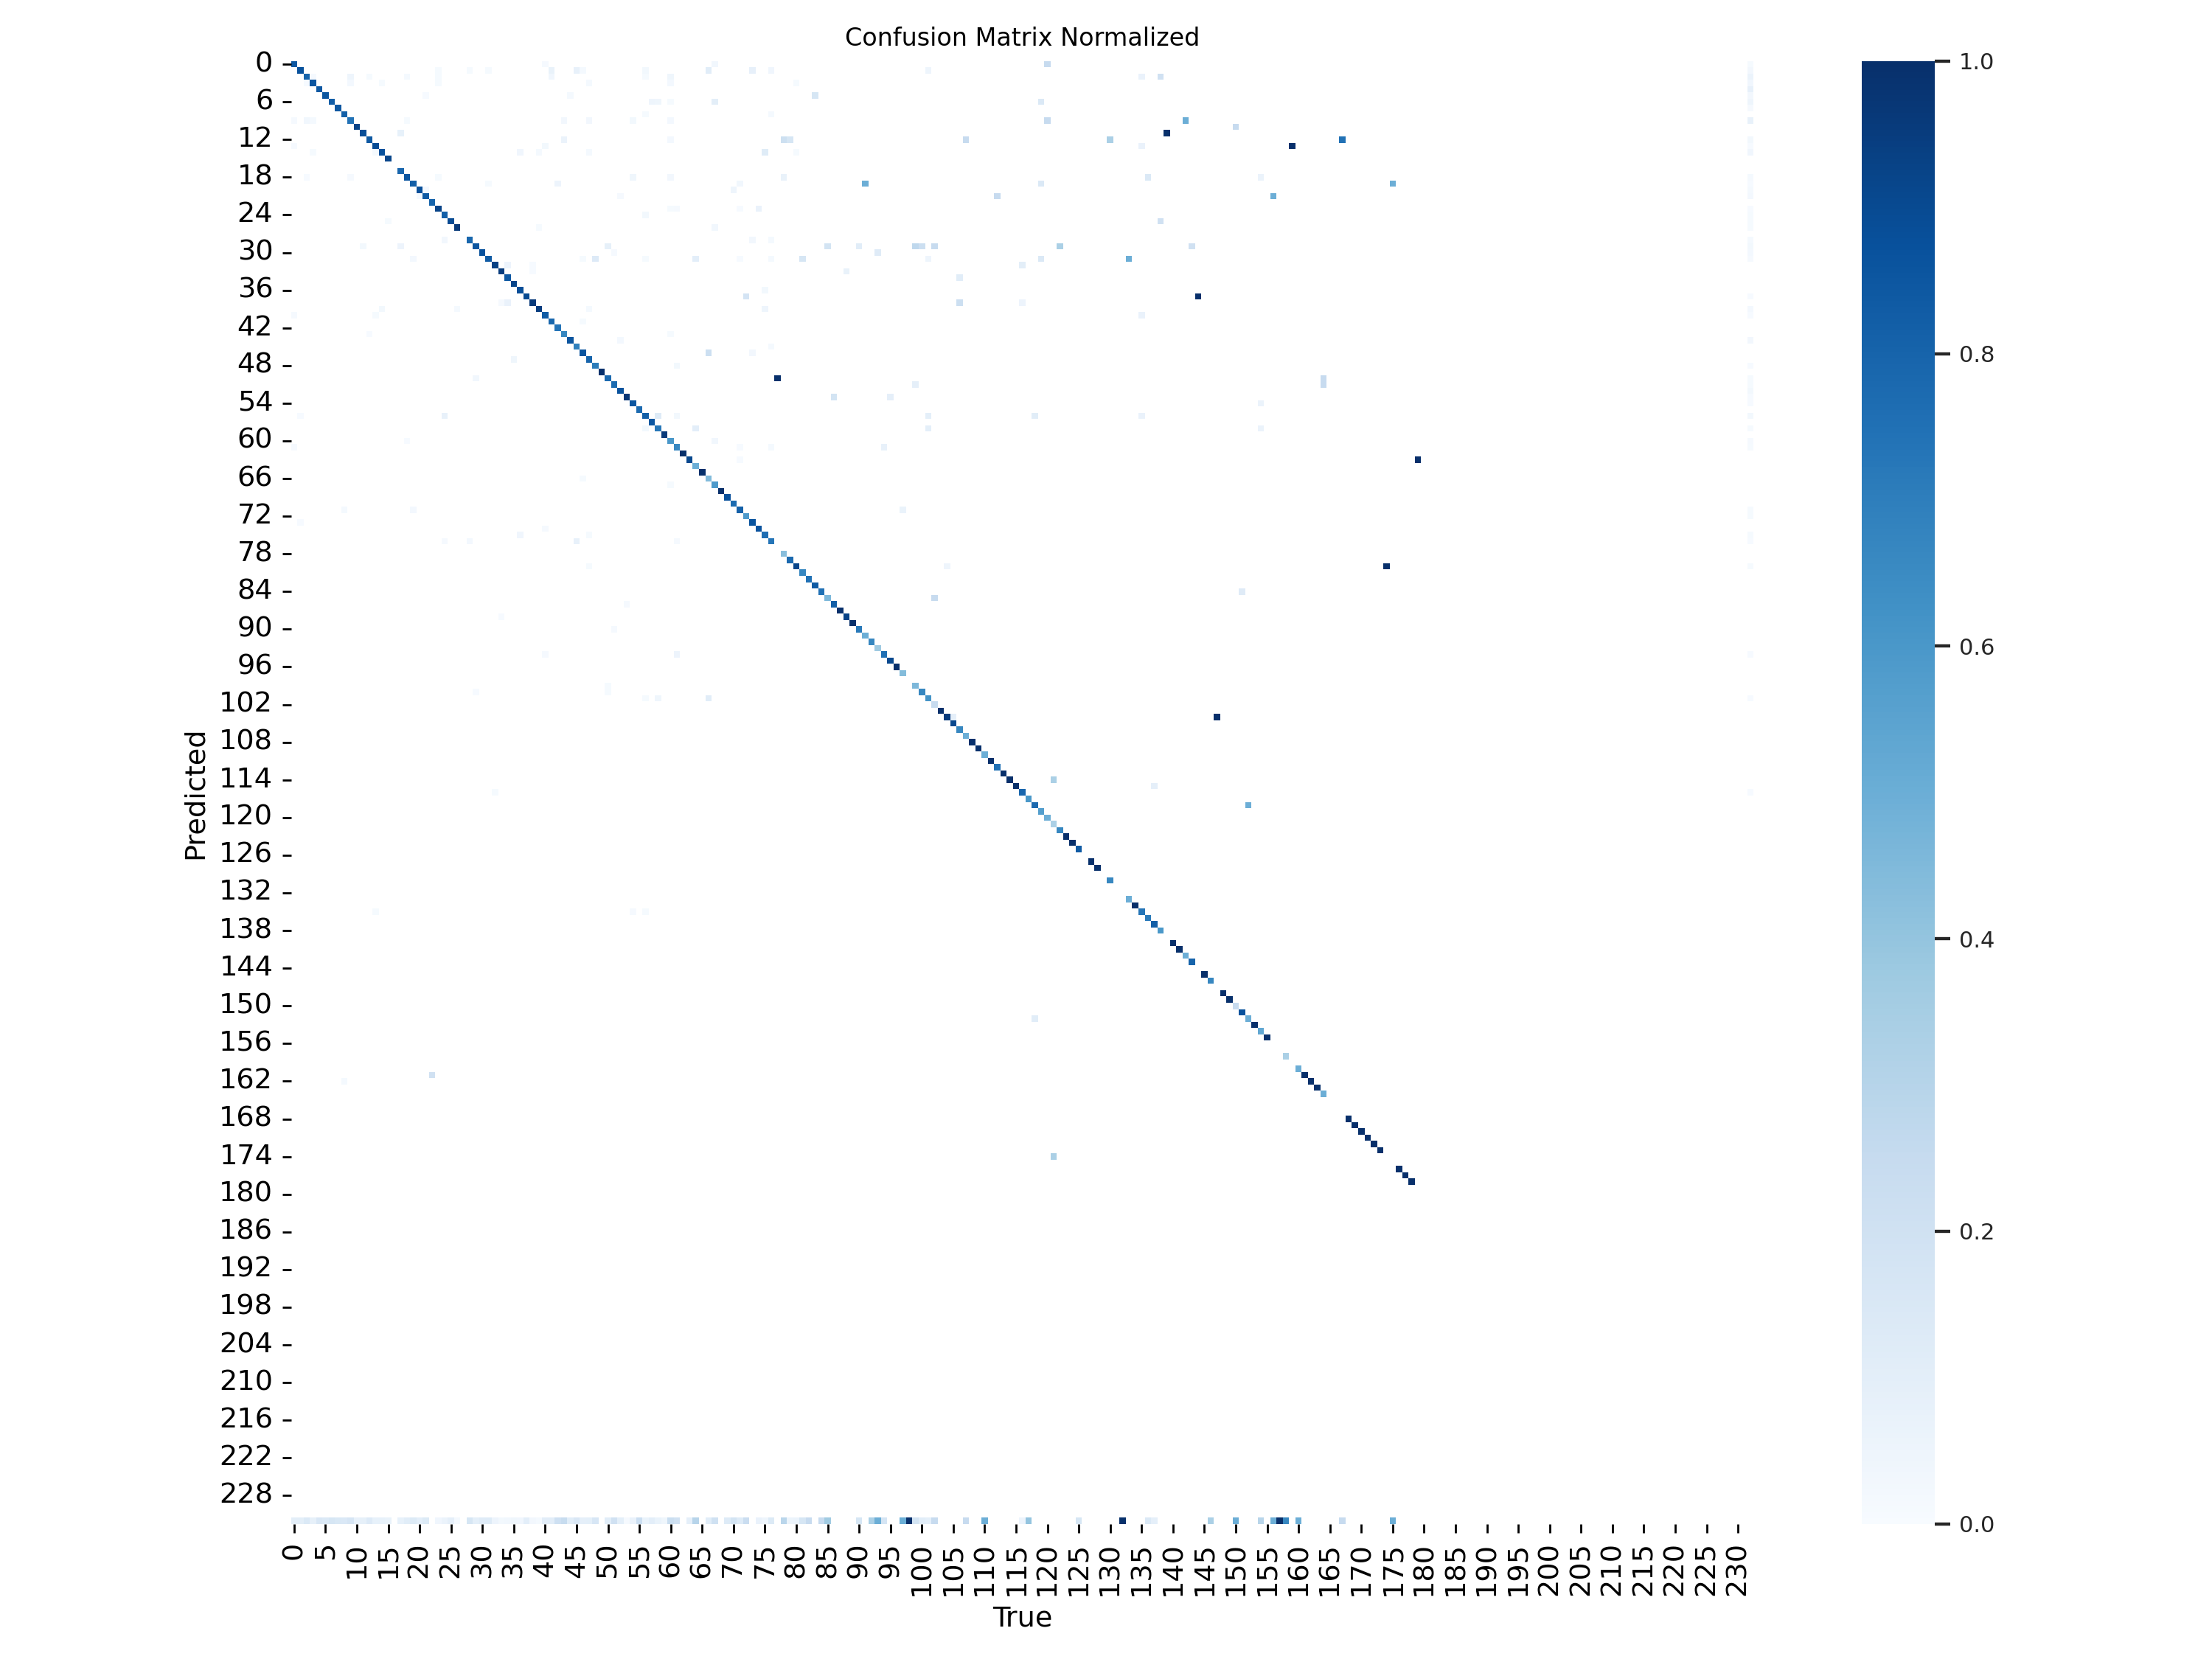
\includegraphics[width=0.4\textwidth]{../figure/tt100k_ex_confusion_matrix_normalized.png}
        }
        \subfloat[YOLOv11s\label{fig:tt100k_11s_cmn}]{
            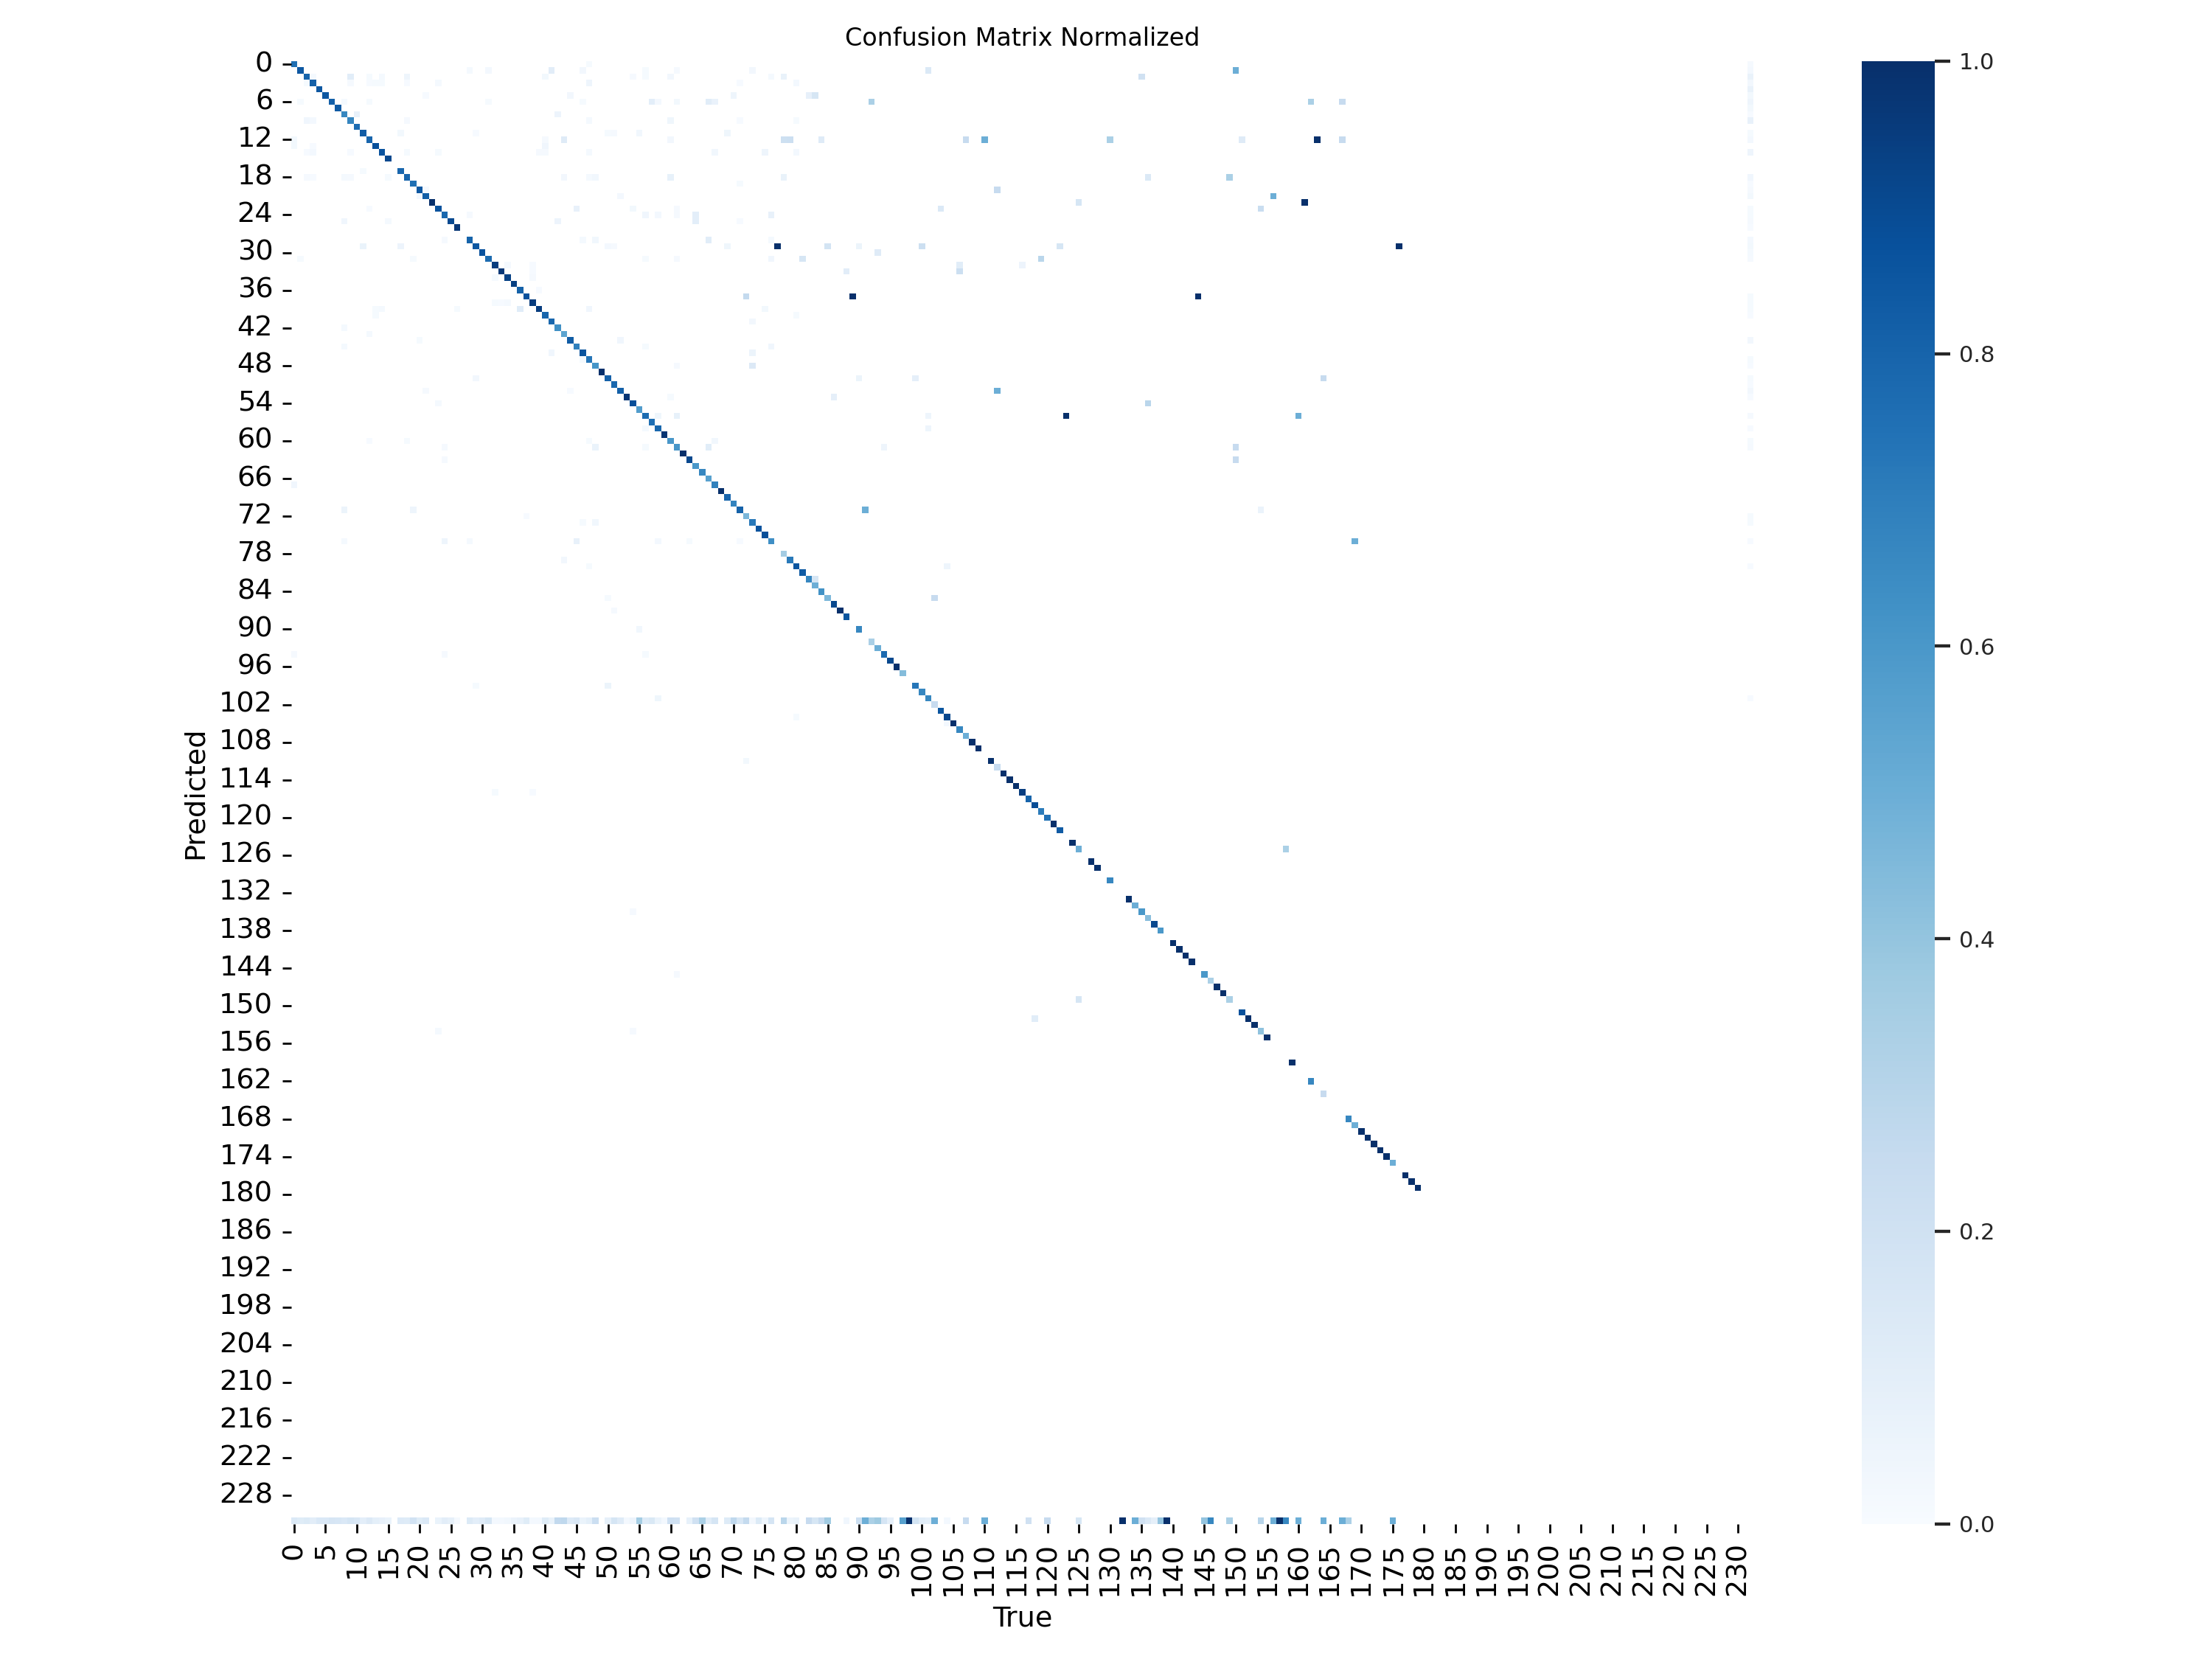
\includegraphics[width=0.4\textwidth]{../figure/tt100k_v11s_confusion_matrix_normalized.png}
        } \\
        \subfloat[YOLOv10s\label{fig:tt100k_10s_cmn}]{
            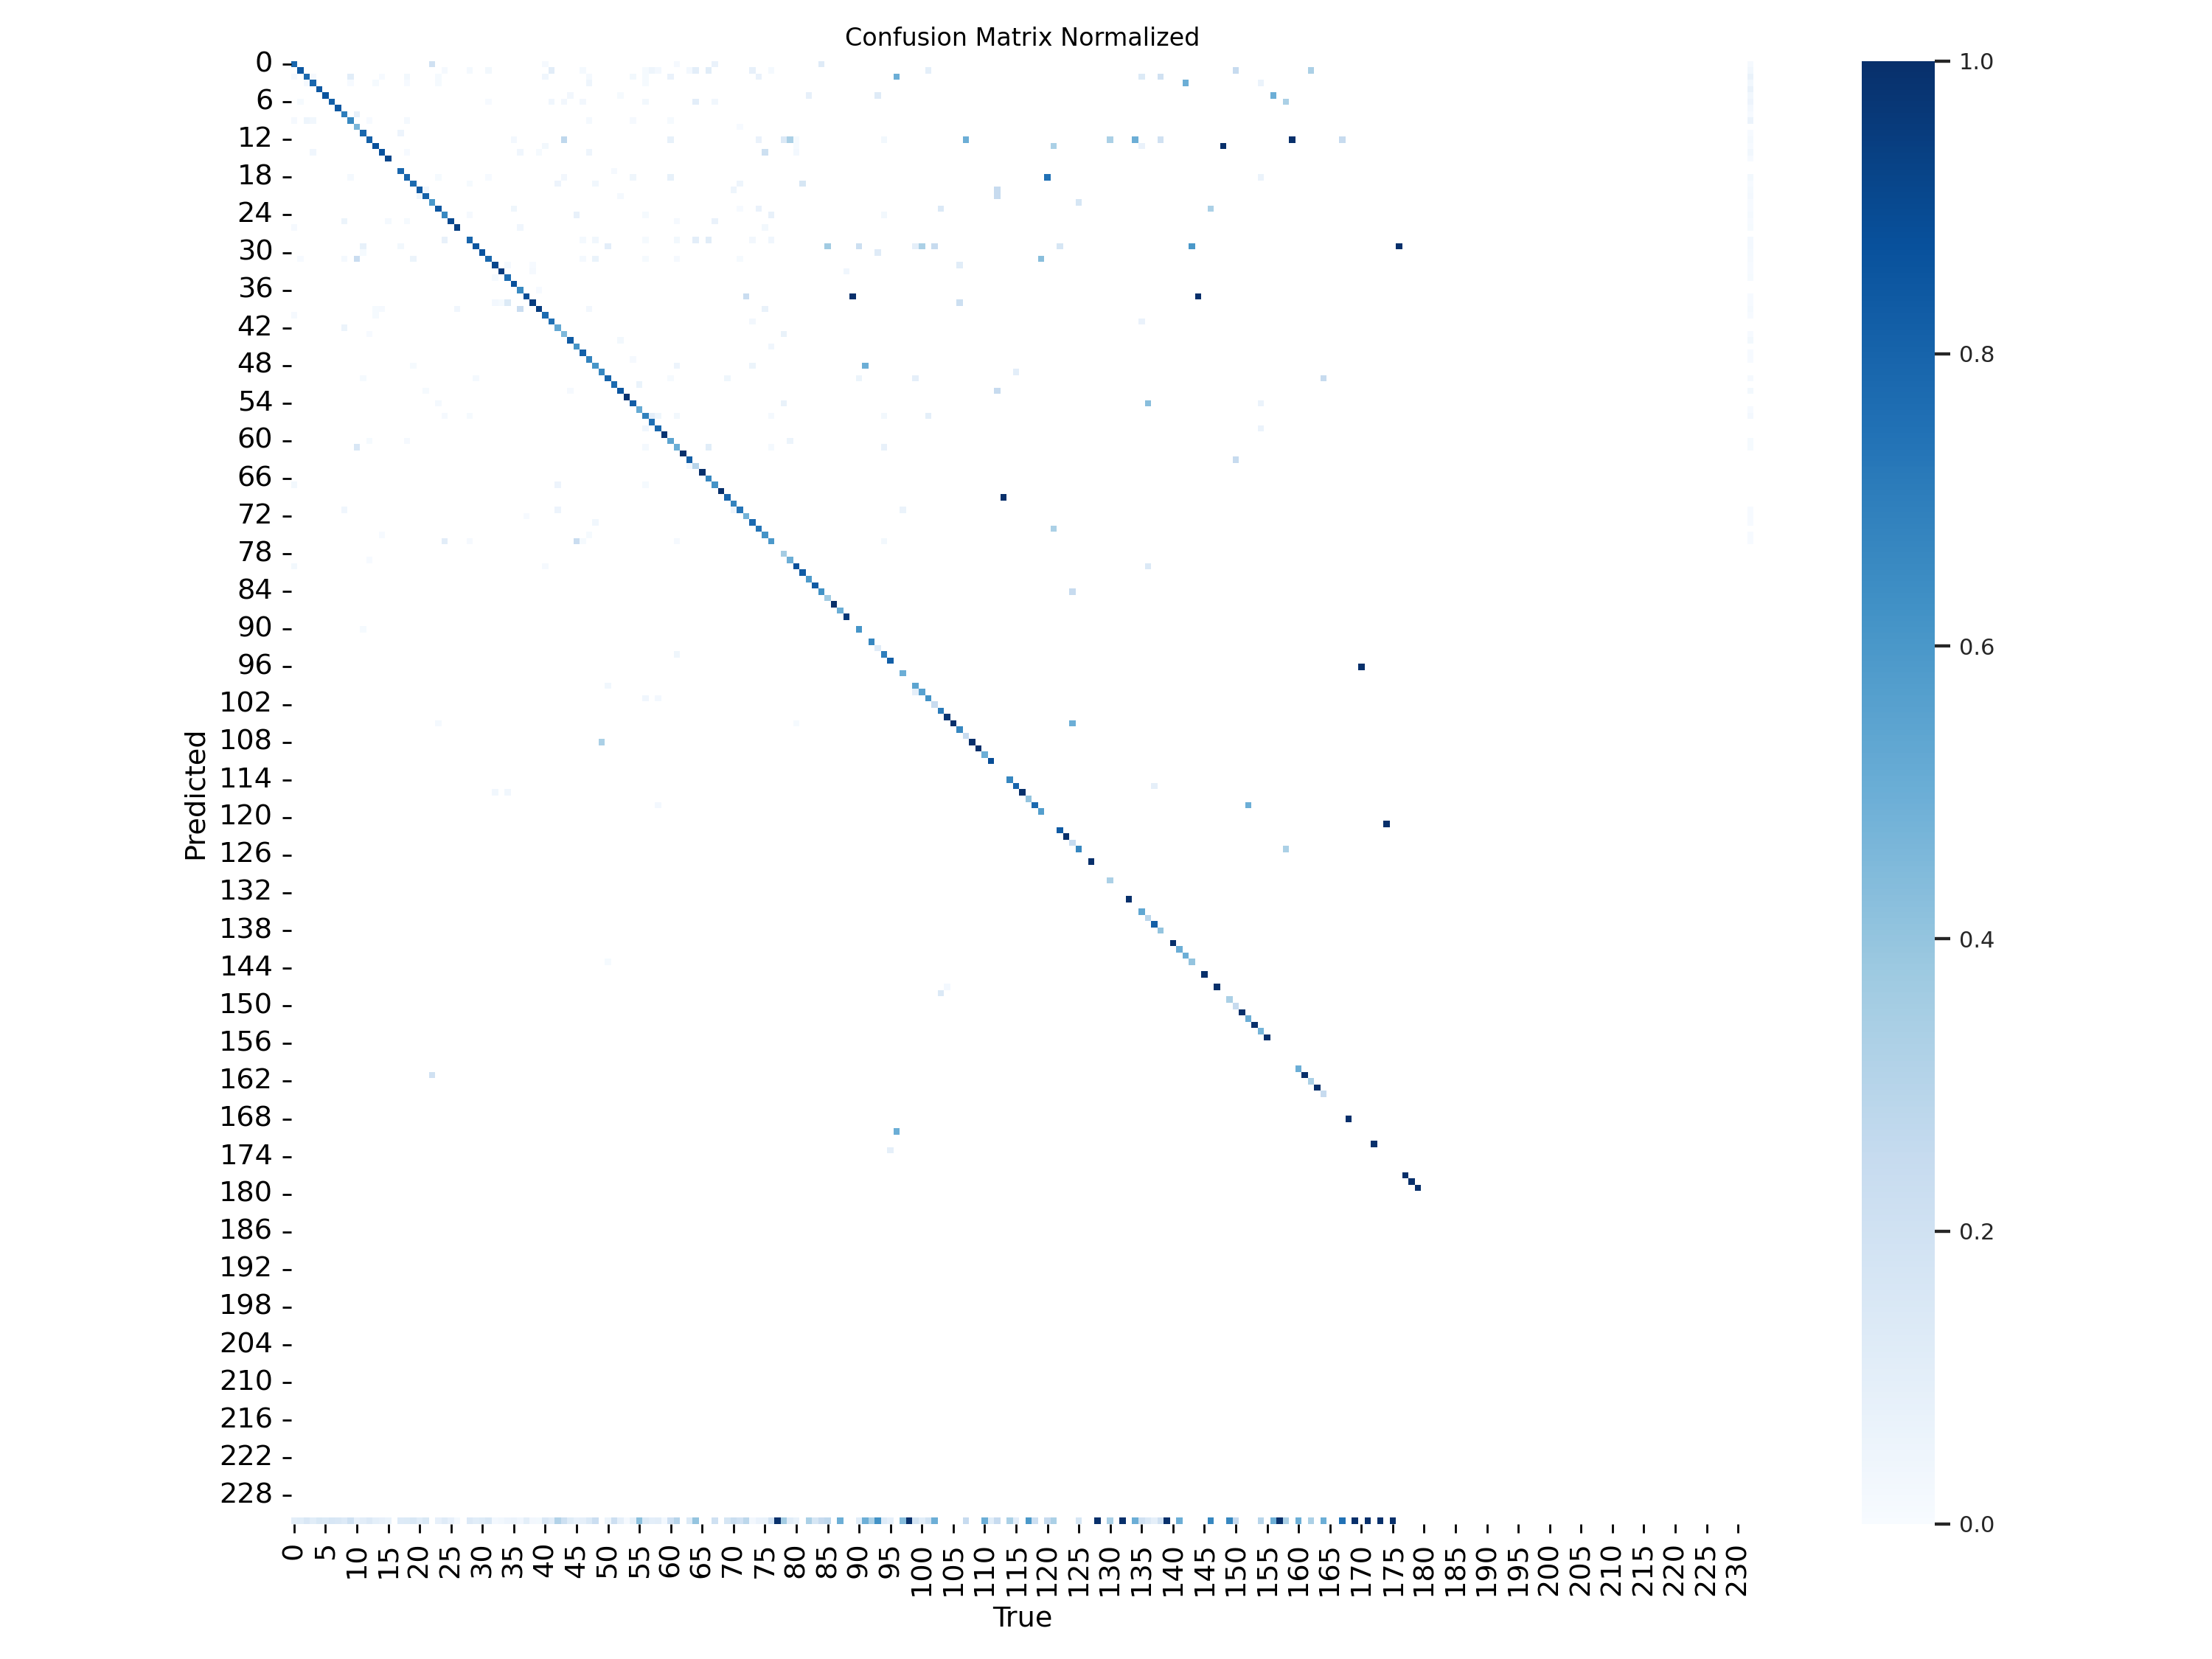
\includegraphics[width=0.4\textwidth]{../figure/tt100k_v10s_confusion_matrix_normalized.png}
        }
        \subfloat[YOLOv9s\label{fig:tt100k_9s_cmn}]{
            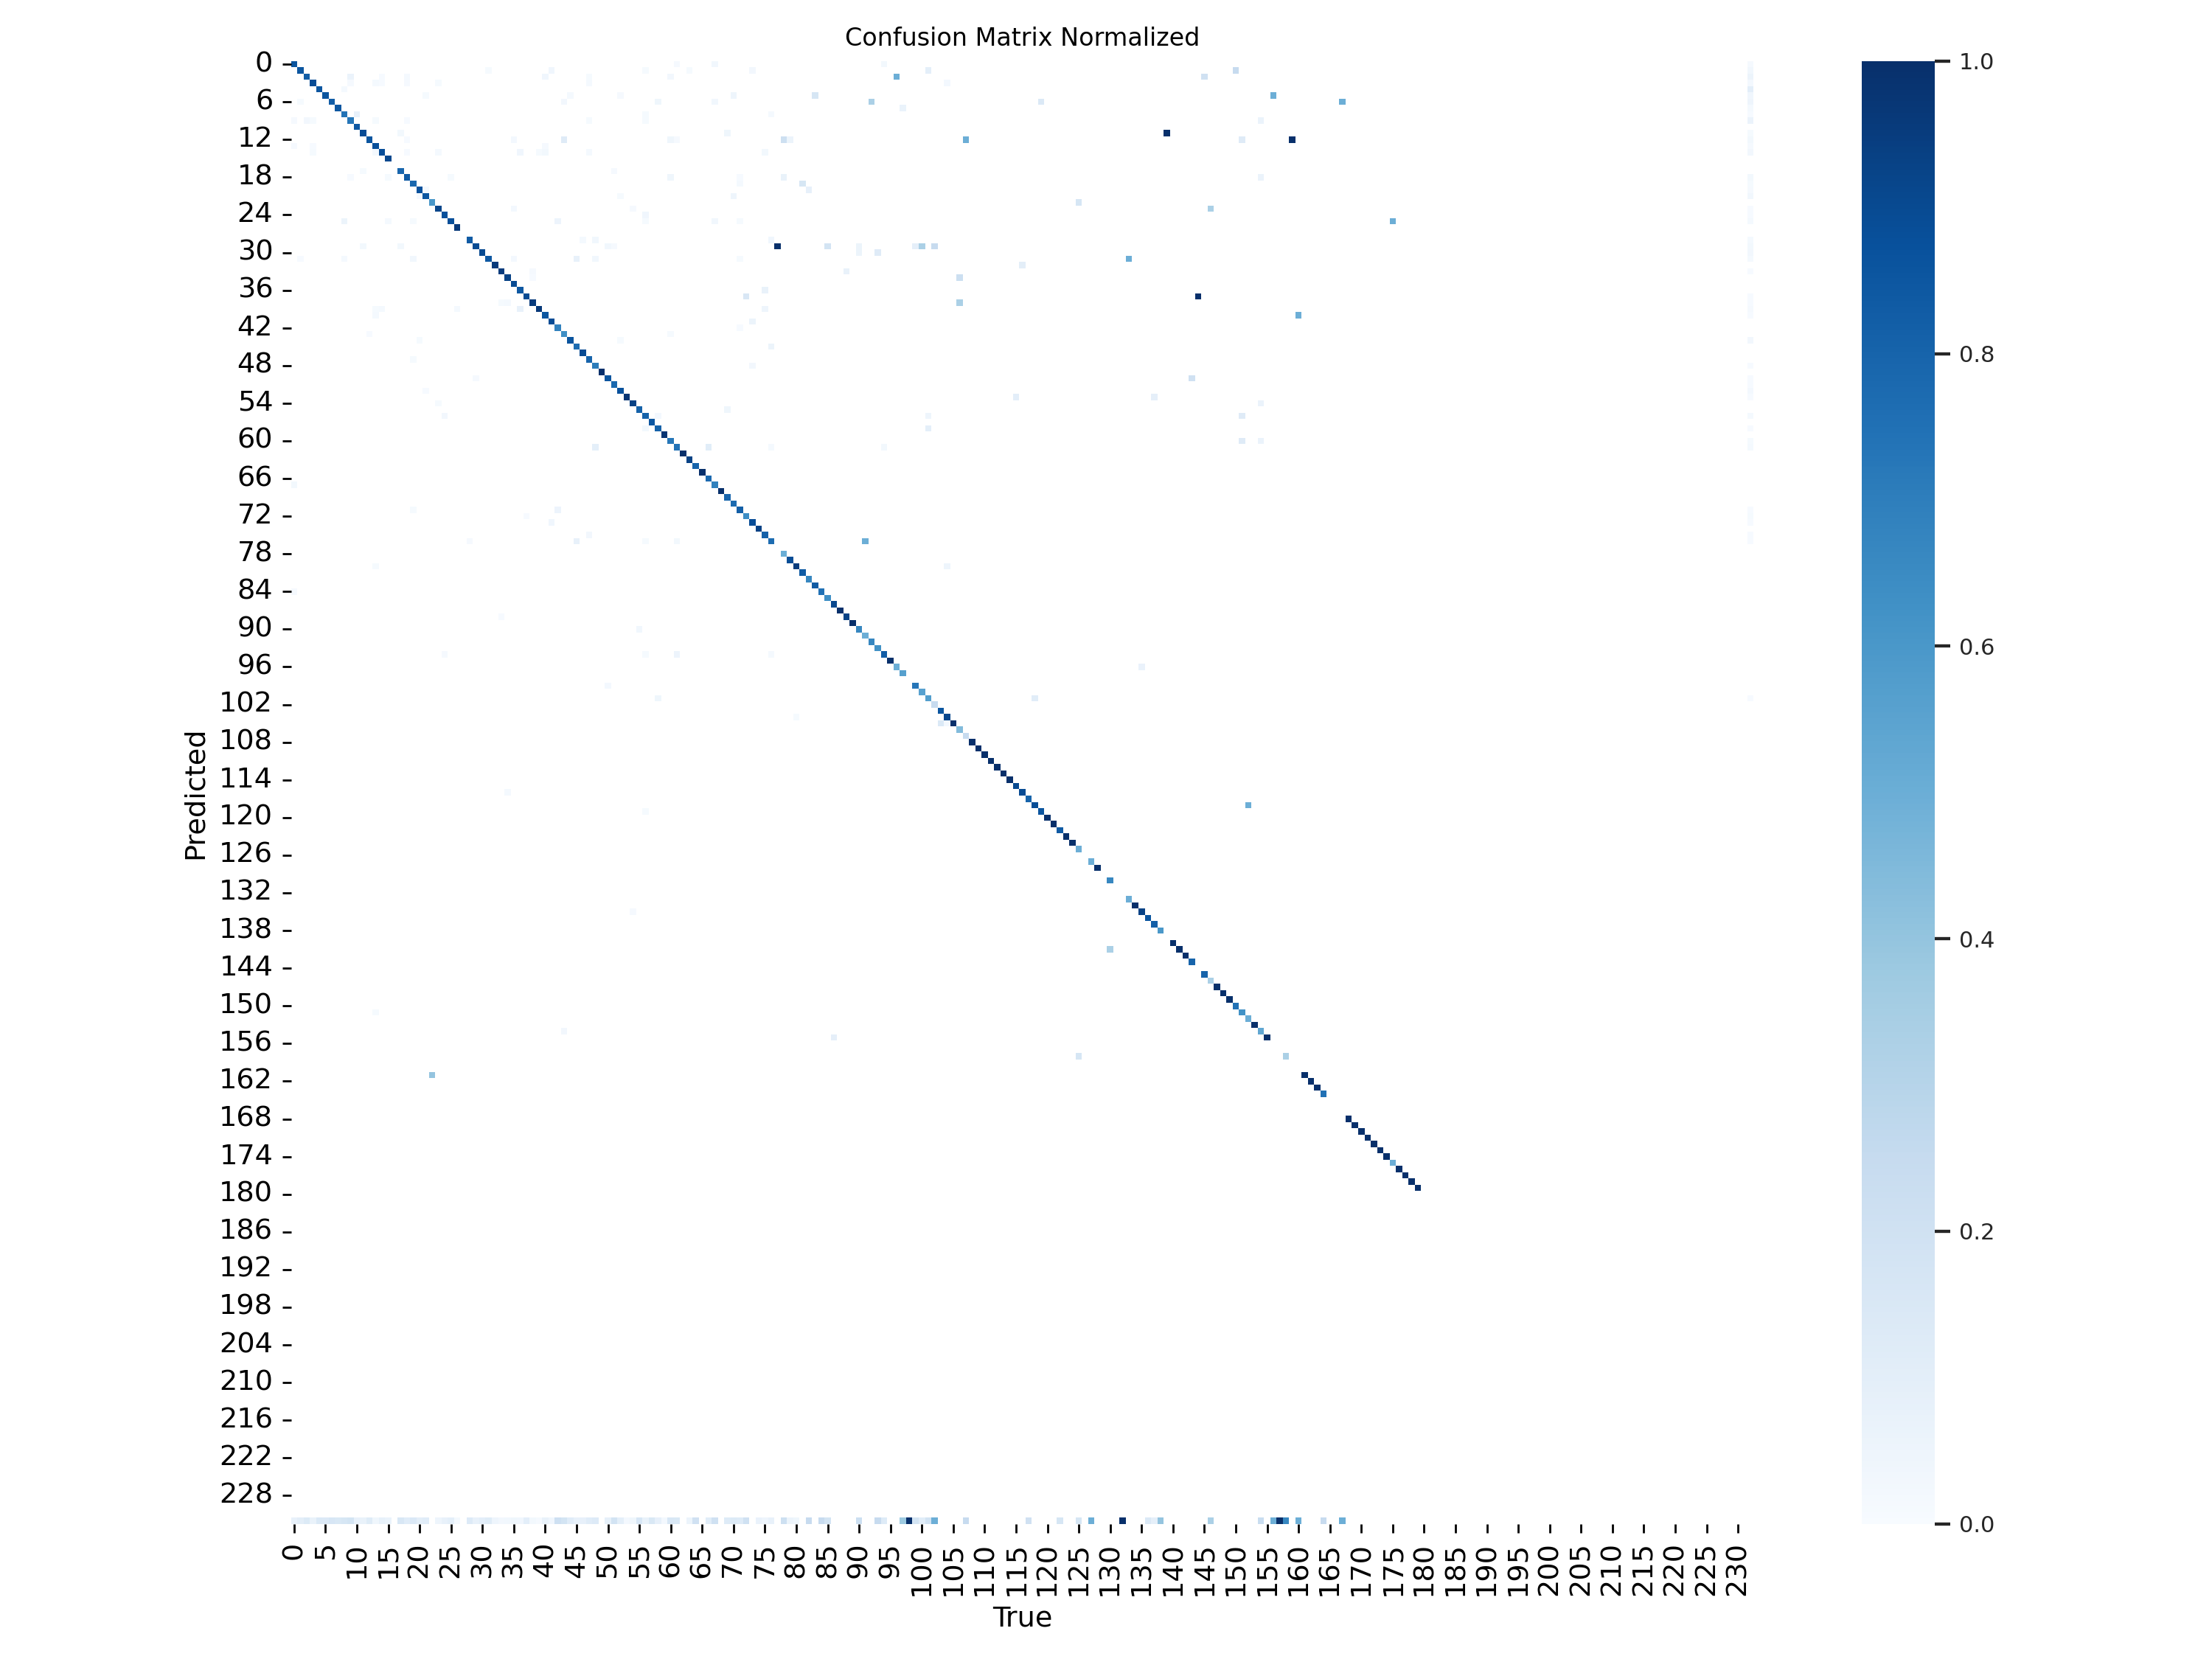
\includegraphics[width=0.4\textwidth]{../figure/tt100k_v9s_confusion_matrix_normalized.png}
        }
    \captionsetup{font=footnotesize}
    \bicaption{不同的网络模型在TT100K数据集上的归一化混淆矩阵}{Symbol cross-reference table}
    \label{fig:tt100k_cmn}
\end{figure}

\begin{figure}[htbp]
    \centering
        \subfloat[EX-YOLO\label{fig:tt100k_ex_f1}]{
            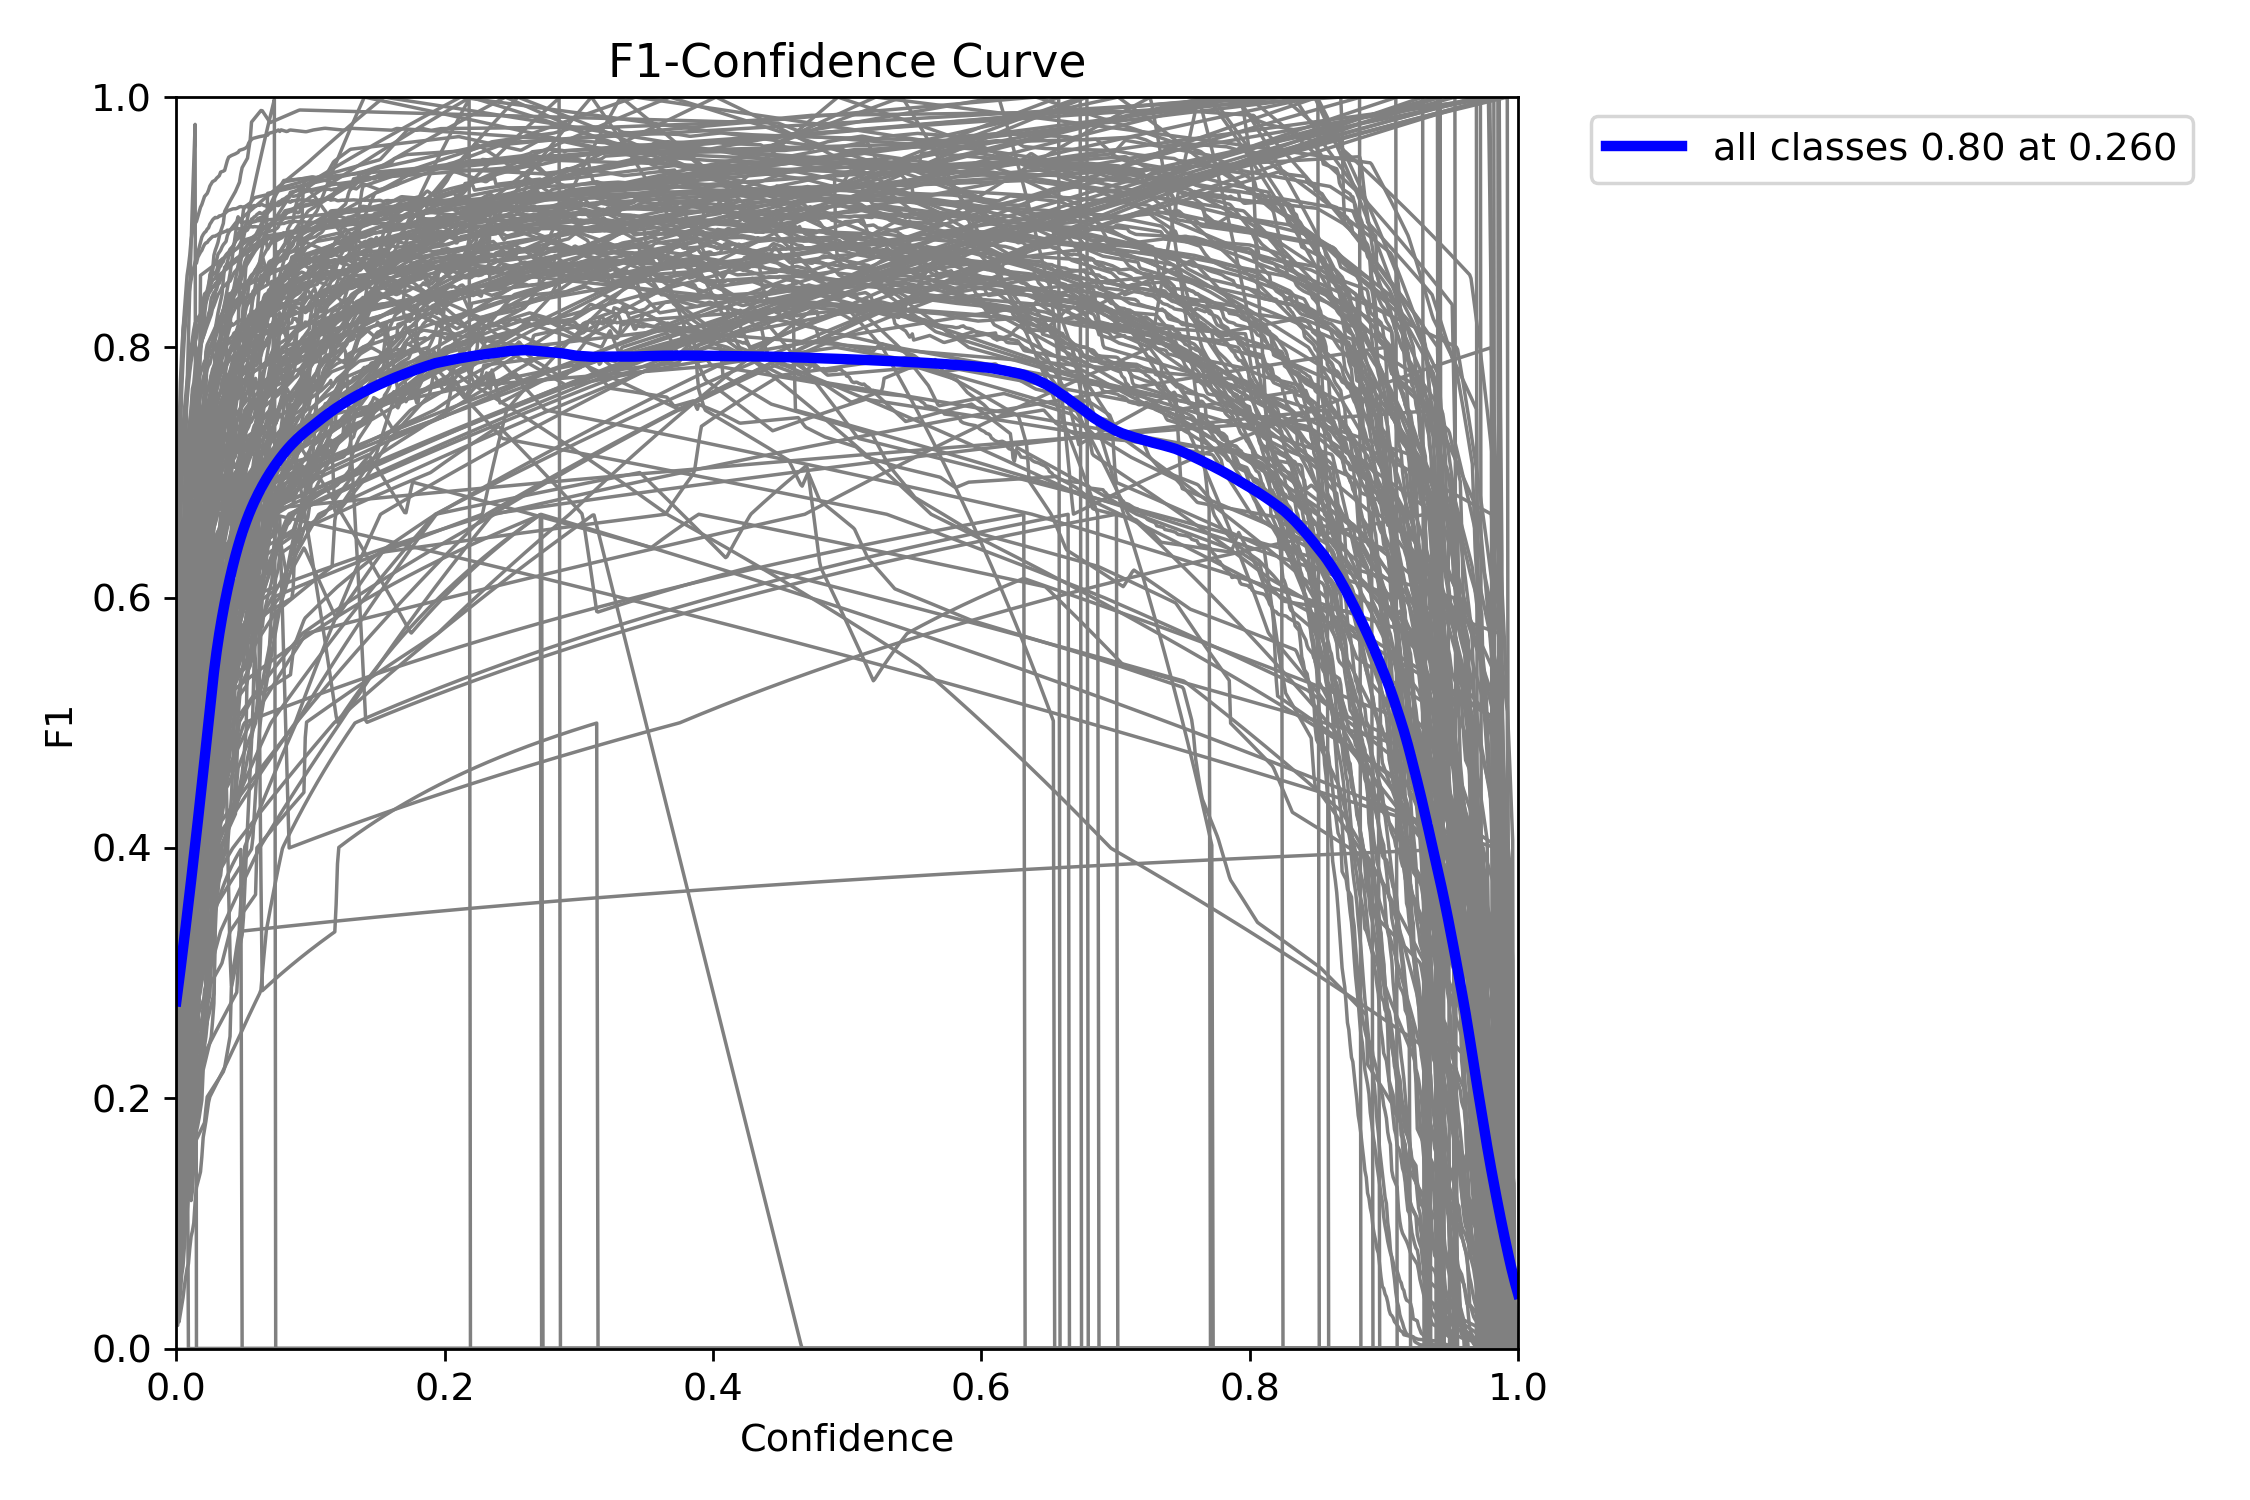
\includegraphics[width=0.4\textwidth]{../figure/tt100k_ex_F1_curve.png}
        }
        \subfloat[YOLOv11s\label{fig:tt100k_11s_f1}]{
            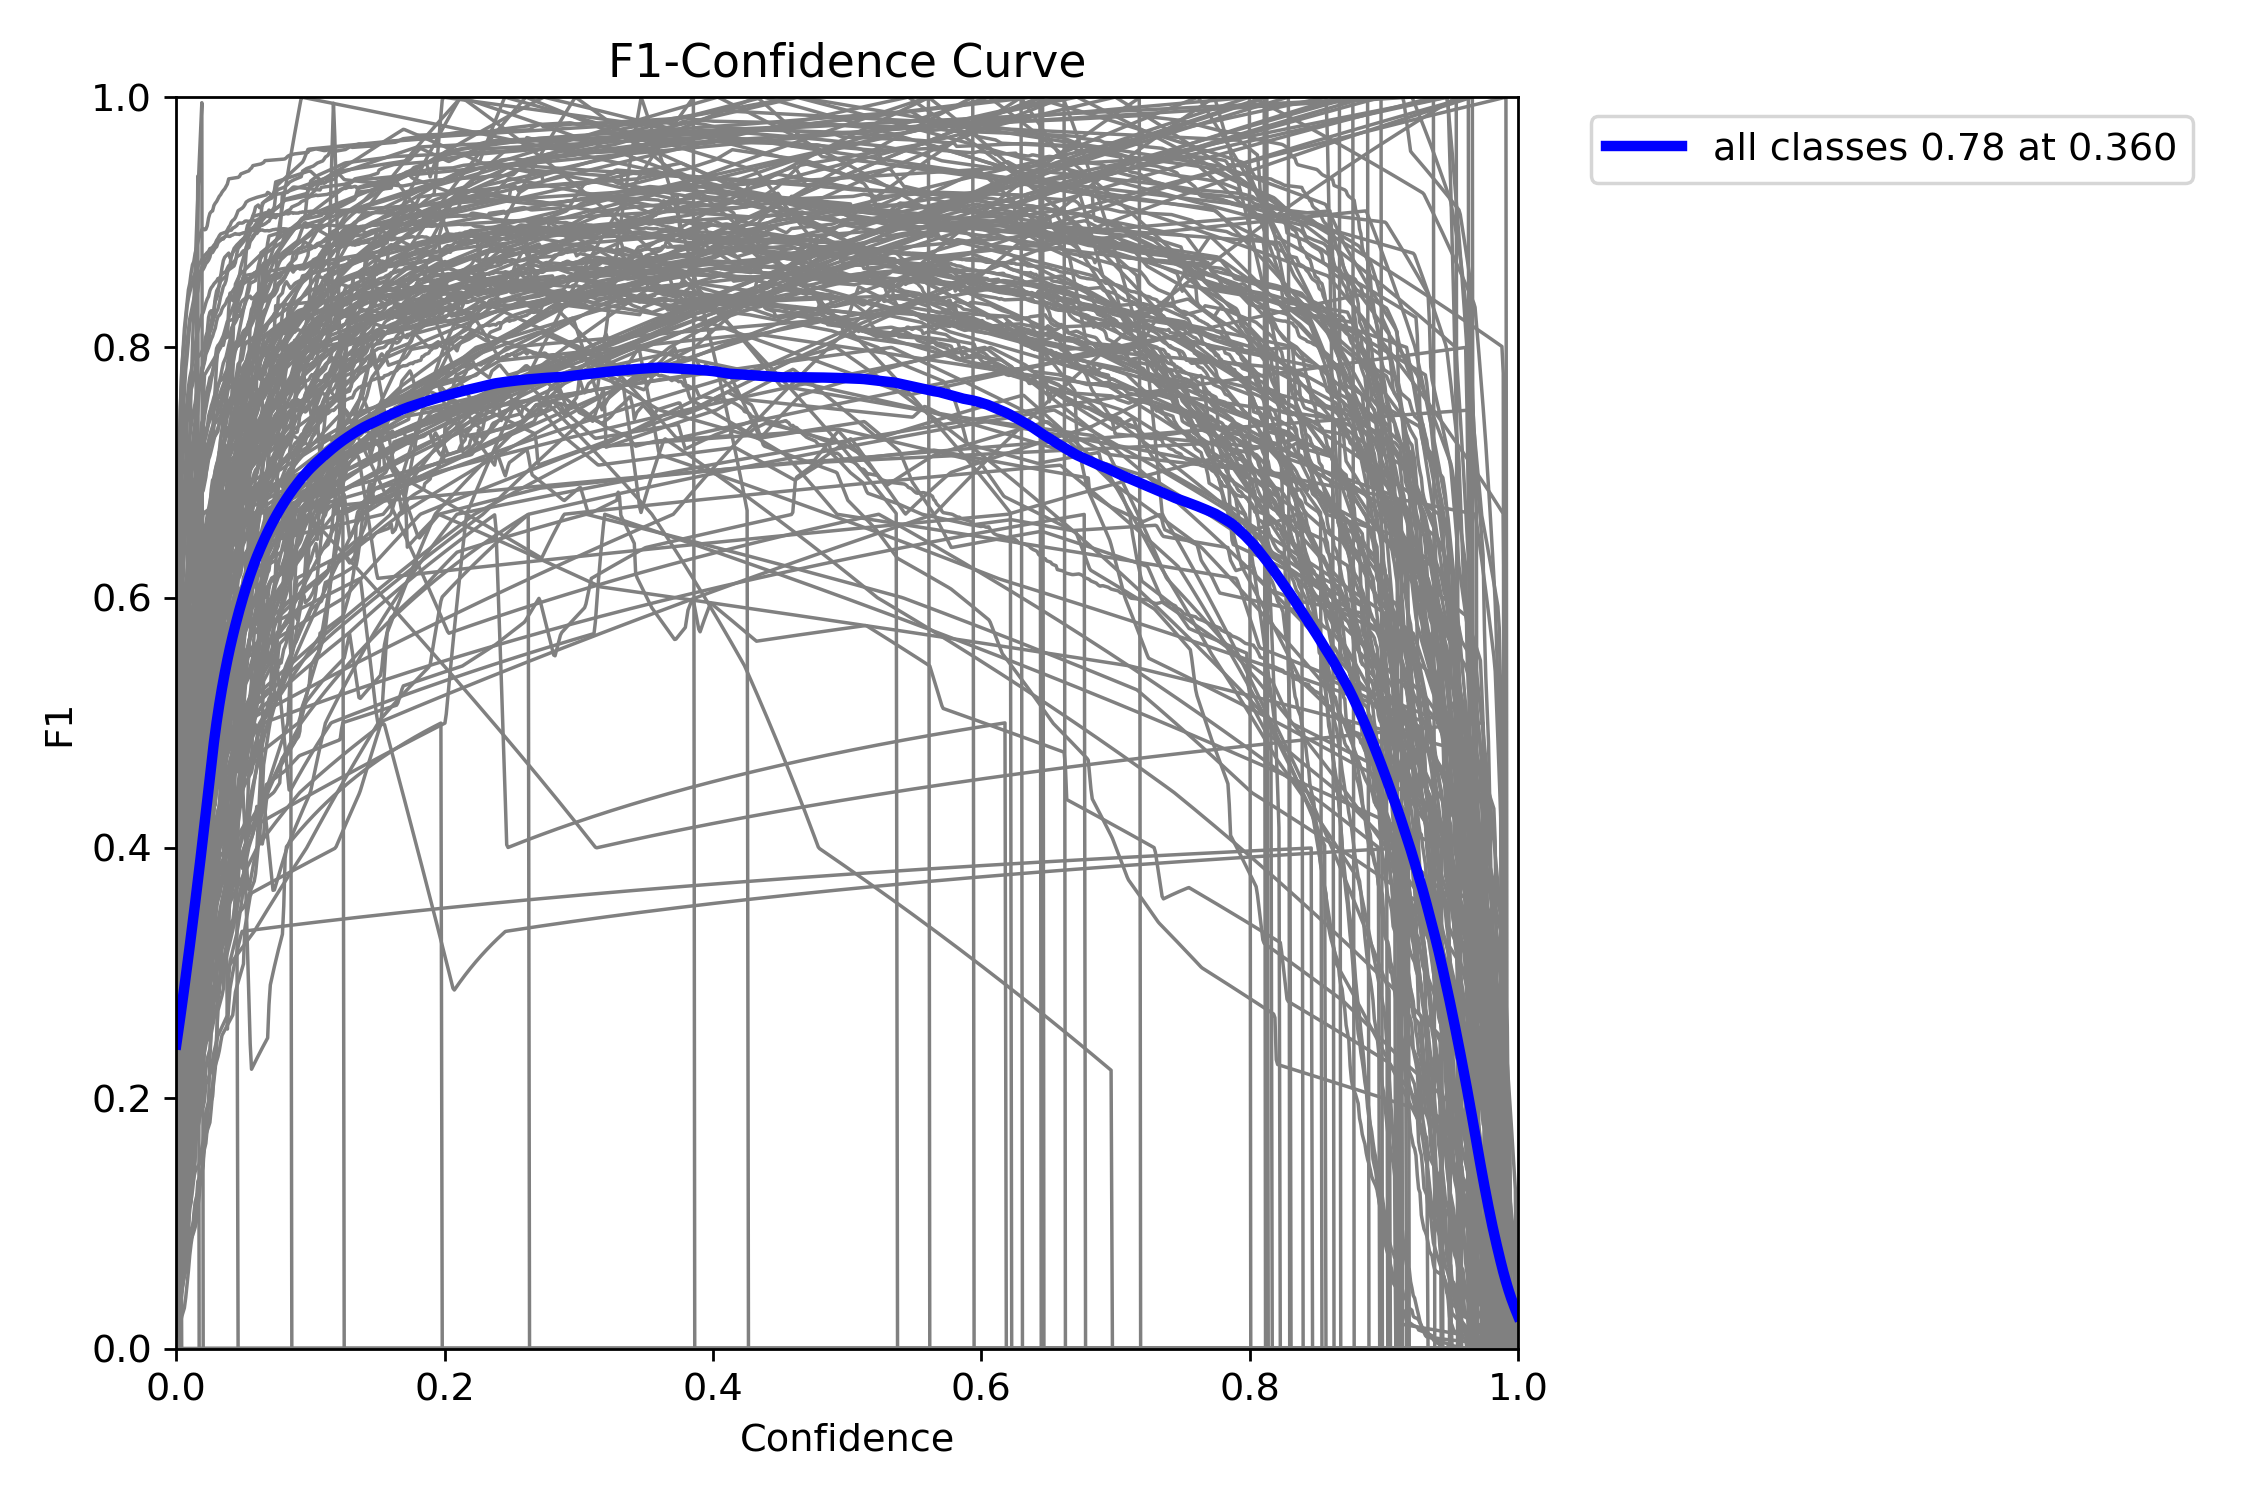
\includegraphics[width=0.4\textwidth]{../figure/tt100k_v11s_F1_curve.png}
        } \\
        \subfloat[YOLOv10s\label{fig:tt100k_10s_f1}]{
            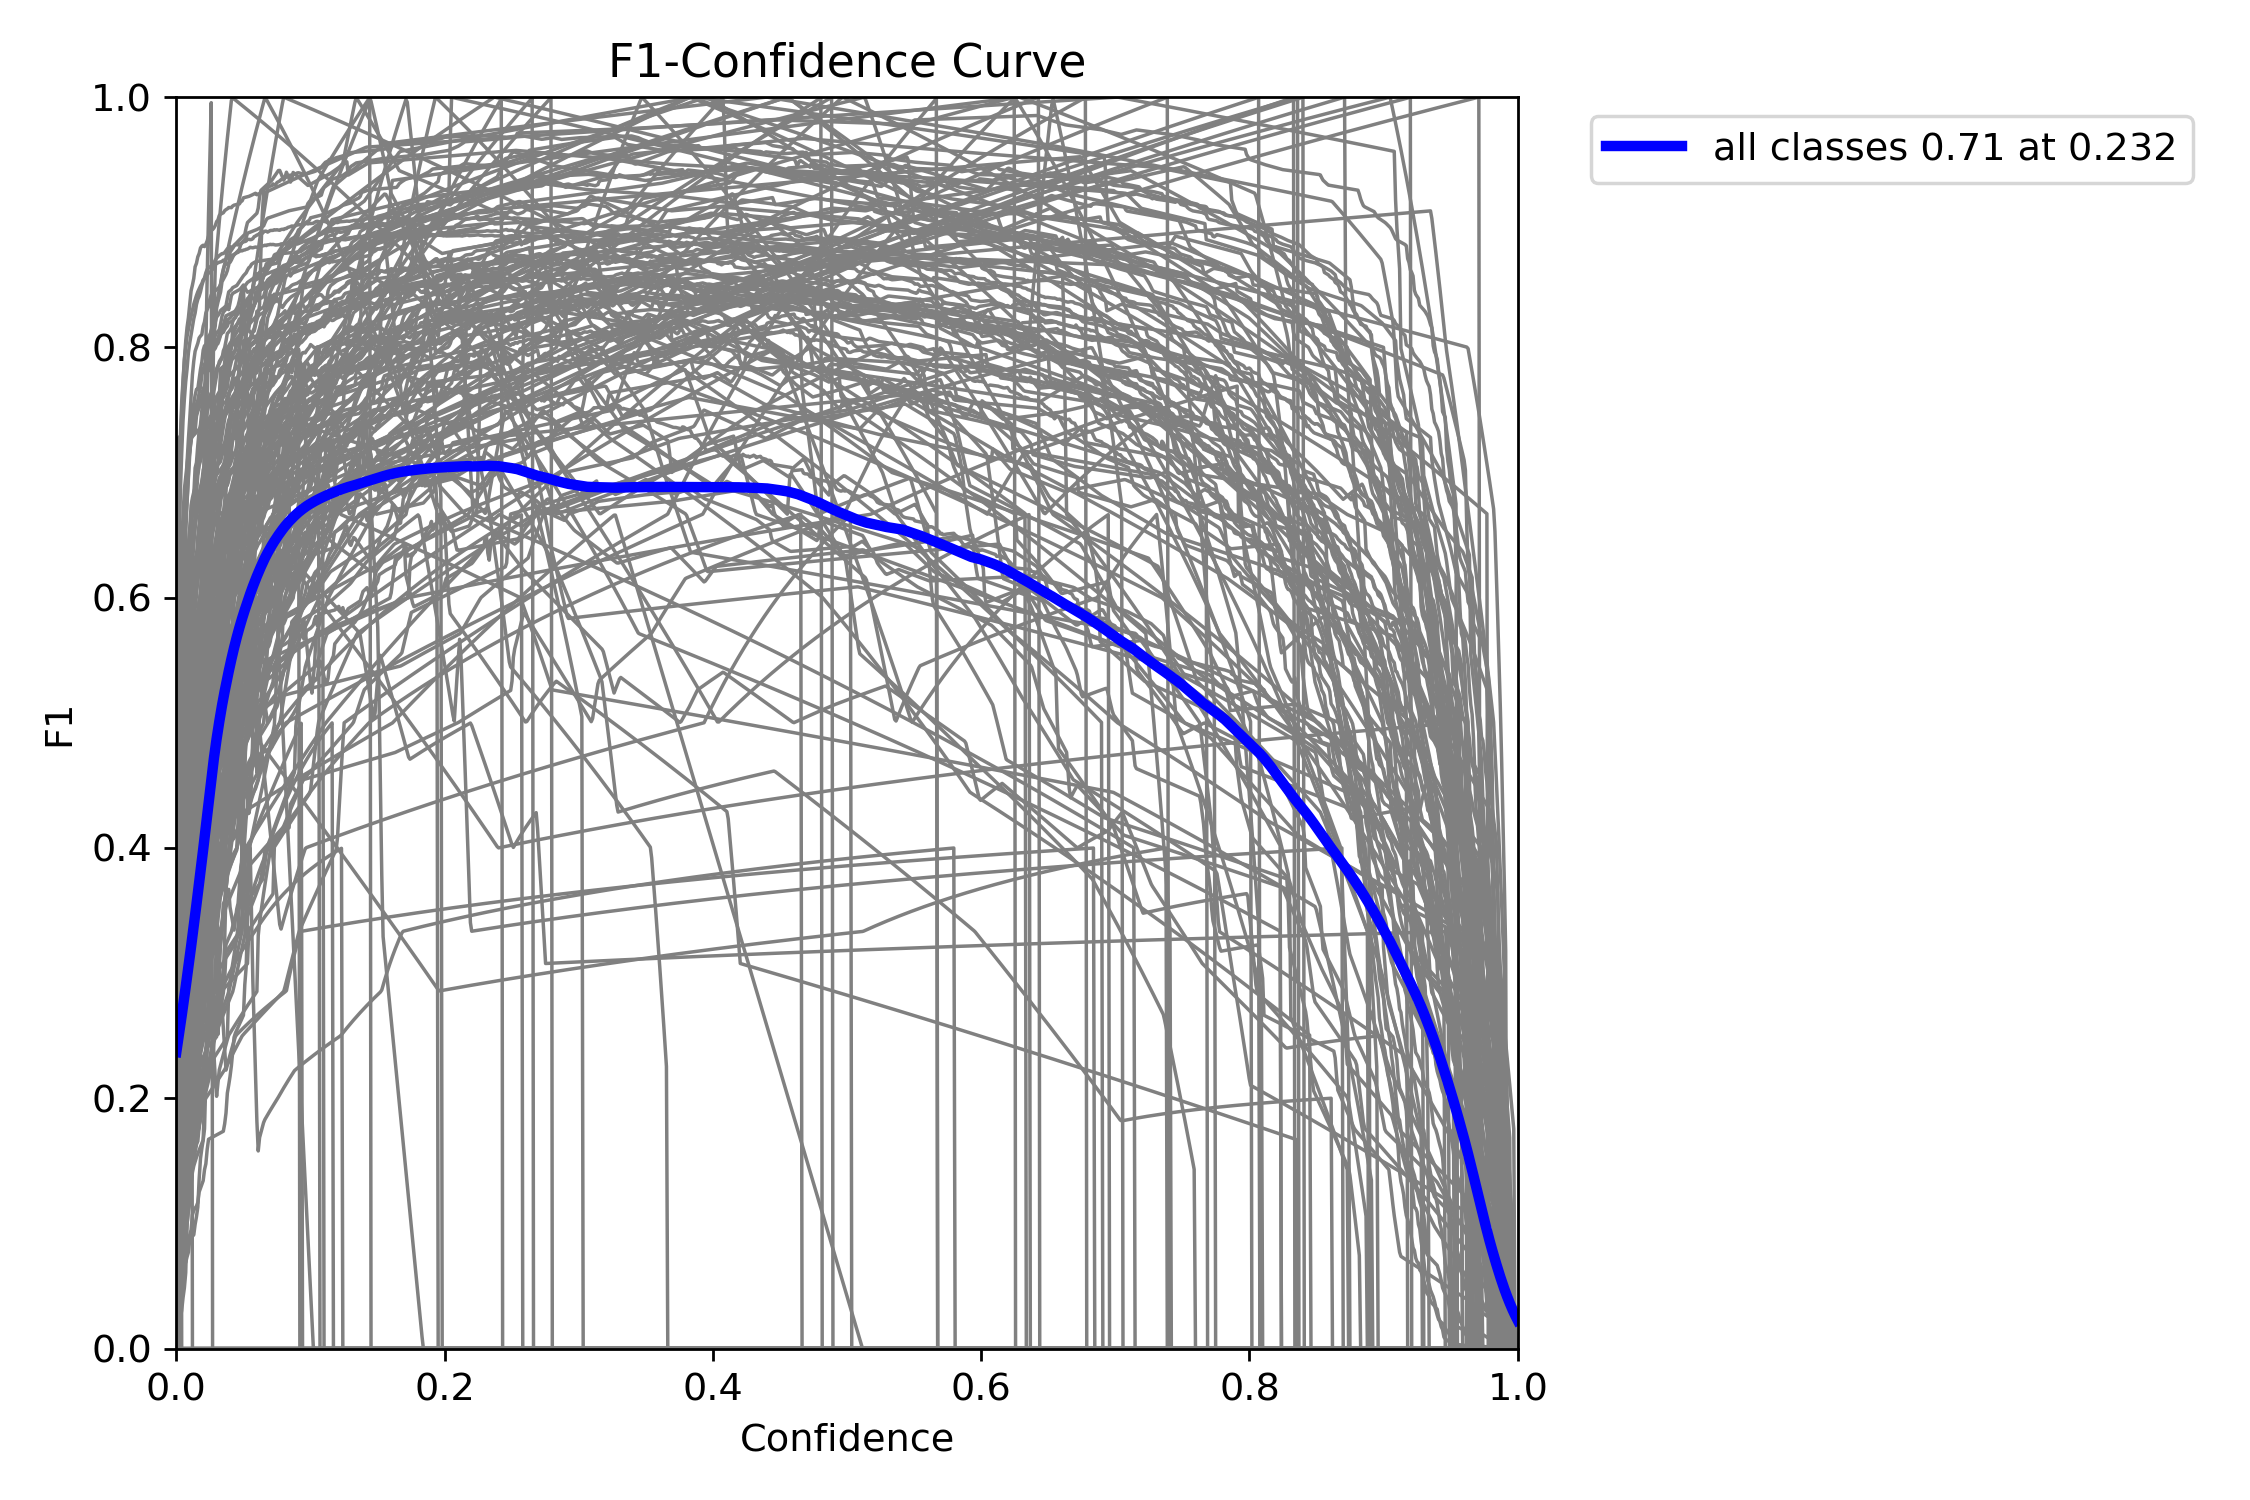
\includegraphics[width=0.4\textwidth]{../figure/tt100k_v10s_F1_curve.png}
        }
        \subfloat[YOLOv9s\label{fig:tt100k_9s_f1}]{
            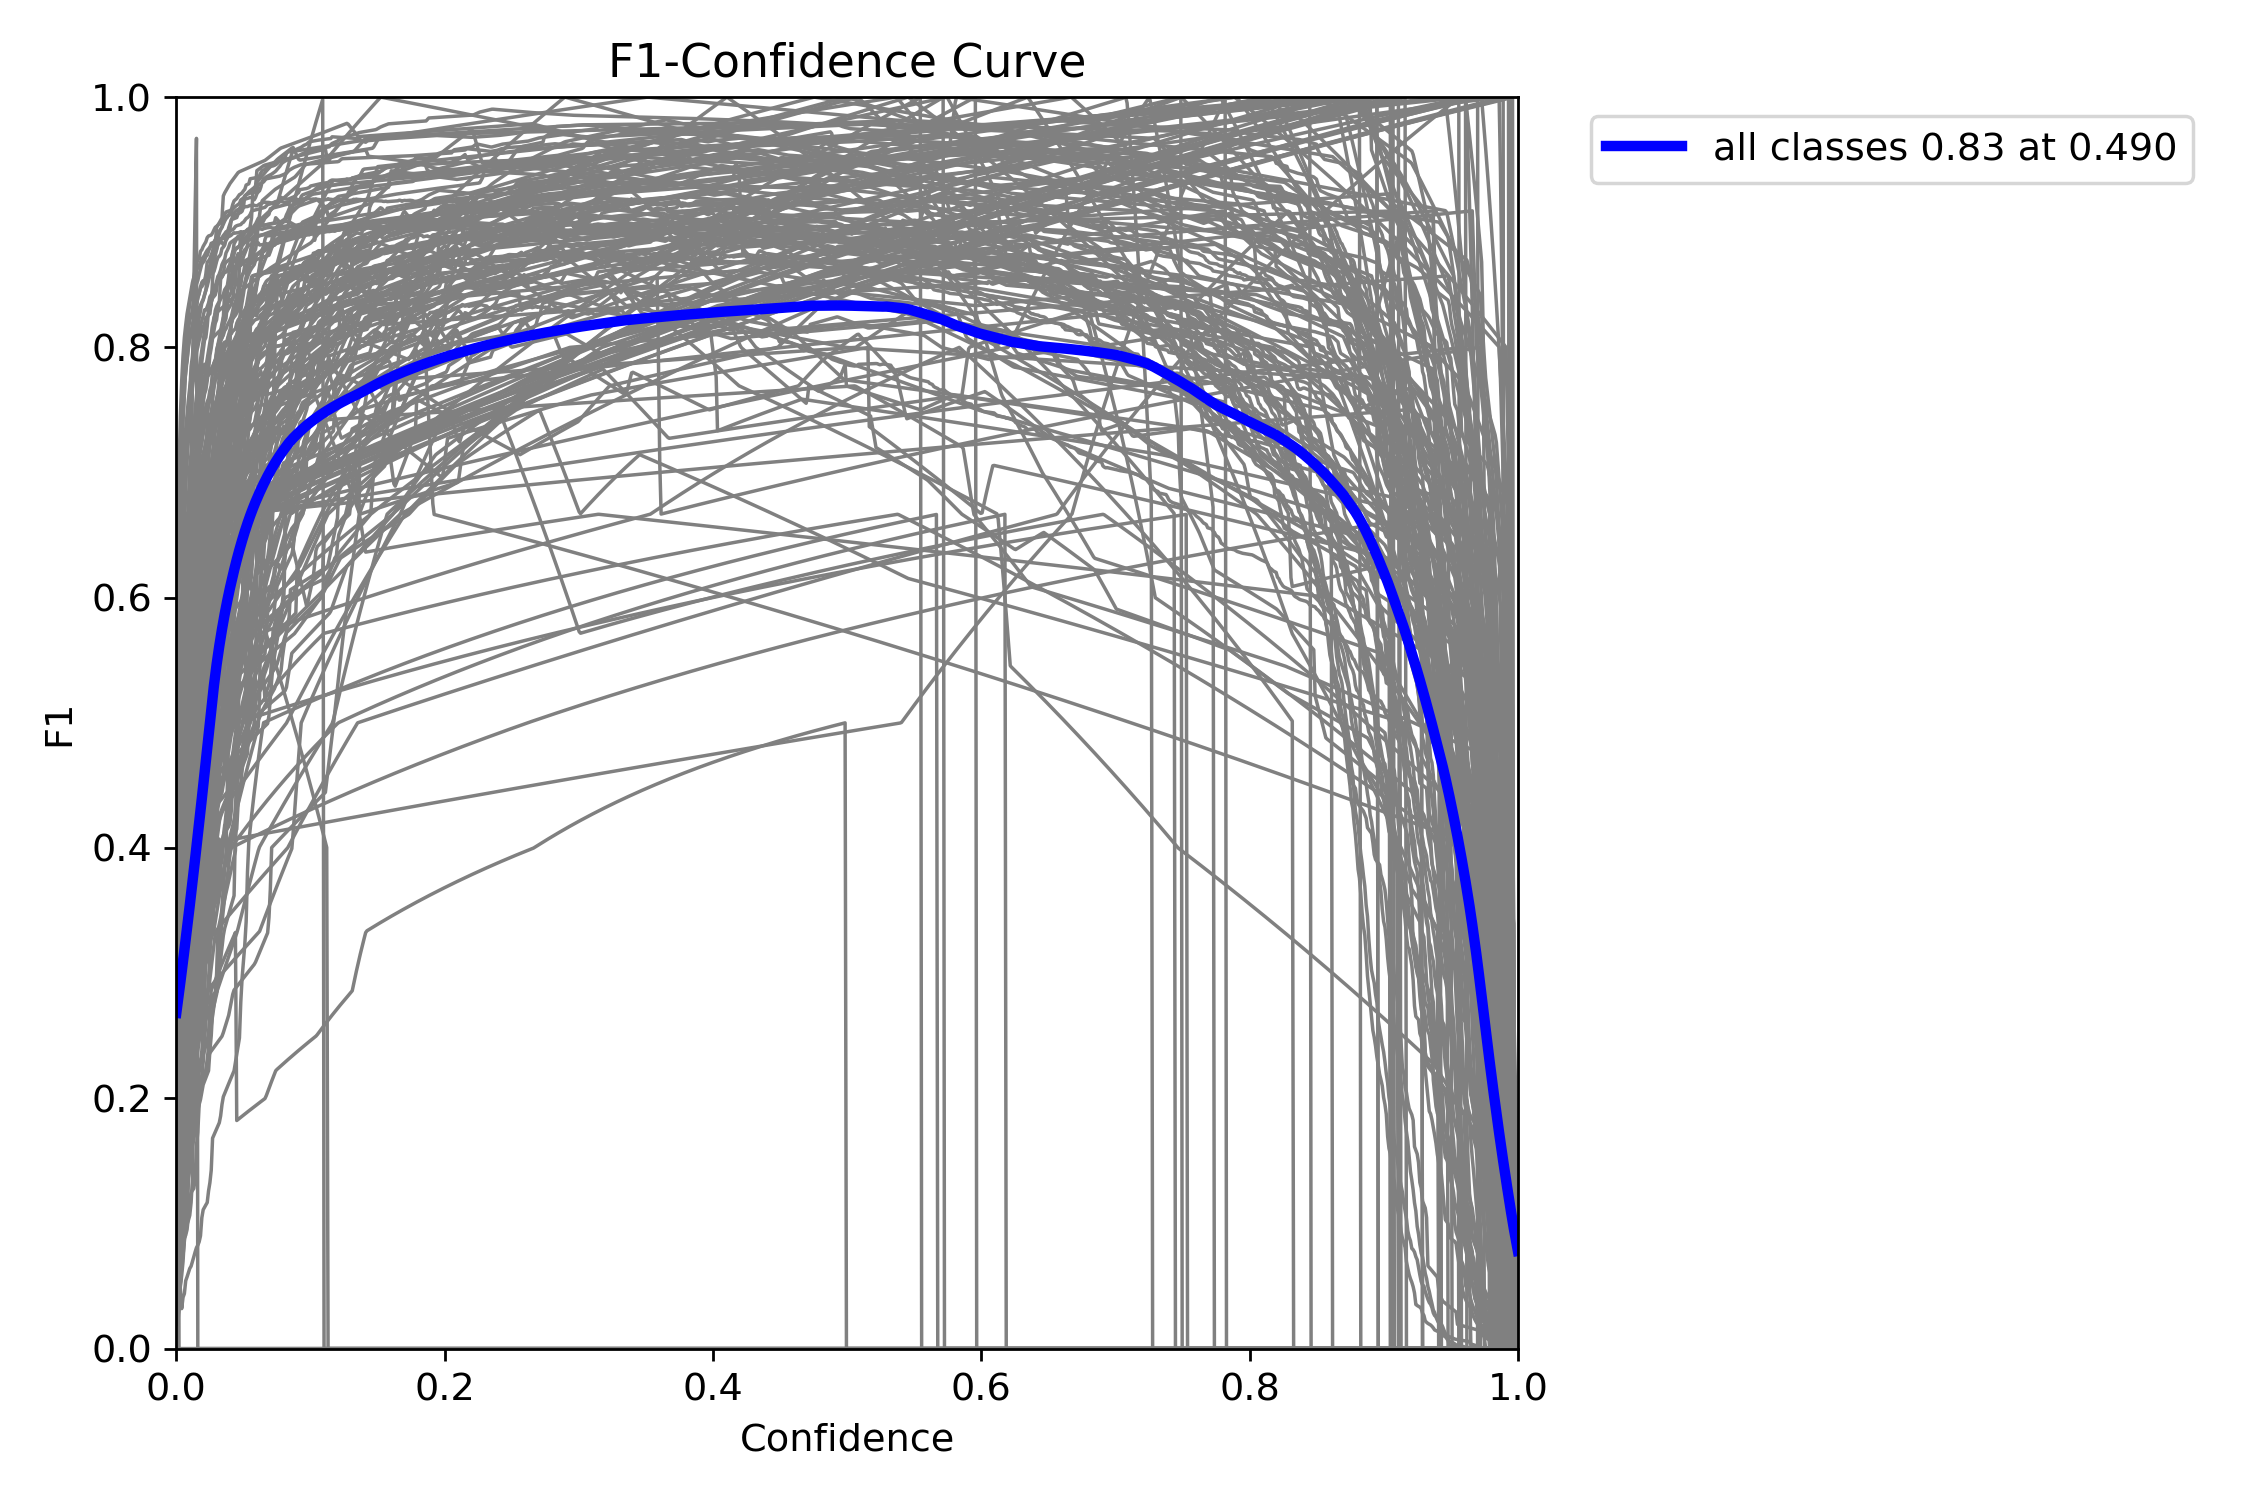
\includegraphics[width=0.4\textwidth]{../figure/tt100k_v9s_F1_curve.png}
        }
    \captionsetup{font=footnotesize}
    \bicaption{不同的网络模型在TT100K数据集上的F1得分}{Symbol cross-reference table}
    \label{fig:tt100k_f1}
\end{figure}

在表 \ref{tab:compare_studies_tt100k} 中,从模型参数来看,YOLOv9s参数容量是最小的,只有7.5MB,而改进后的模型参数容量相对较大,为11.4MB。
虽然our 模型在参数方面有所增加,但在计算量(GFLOP)方面显示出显著优势。
它的计算量只有17.0GFLOPs,远远低于YOLOv11s的21.8GFLOPs、YOLOv10s的25.4GFLOPs和YOLOv9s的27.2GFLOPs。
这表明our 模型在设计中更加关注计算效率。
通过优化算法结构和引入高效模块,它有效地降低了模型的计算复杂性。

在精度(P)方面,YOLOv9s表现最好,为0.914,our 模型为0.875,略低于YOLOv11s的0.878,但高于YOLOv10s的0.776。
在召回(R)方面,our 模型达到了0.830,高于0.777的YOLOv11s、0.752的YOLOv10s和0.818的YOLOv9s。
在mAP性能方面,YOLOv9s以0.906的$mAP_{0.5}$领先,但our 模型紧随其后,达到0.893的$mAP_{0.5}$,明显高于YOLOv11s的0.877和YOLOv10s的0.850。
这表明our 模型在小型目标检测任务中具有很强的竞争力,这可以有效地提高无人机对交通标志等小型目标的检测精度。
虽然与YOLOv9s存在一定的差距,但考虑到我们模型的计算量大幅减少,这种差距在实际应用中是可以接受的,our 模型在精度和效率之间实现了良好的平衡。

图 \ref{fig:tt100k_cmn} 呈现了 YOLOv9s、YOLOv10s、YOLOv11s 以及 our 模型在TT100K数据集针对不同类别目标的预测状况。具体而言,图 \ref{fig:tt100k_cmn} 为归一化混淆矩阵的热力图形式,其中颜色深浅与预测概率呈正相关,颜色愈深,意味着预测准确率愈高,相应地,颜色愈浅,则表明预测准确率较低。需要强调的是,热力图对角线上的数据对应着模型成功预测正确标签的情况,而非对角线部分的数据则反映了模型出现标签预测错误的情形。

然而,从直观观察的角度来看,图 \ref{fig:tt100k_ex_cmn}、图 \ref{fig:tt100k_11s_cmn}、图 \ref{fig:tt100k_10s_cmn} 以及图 \ref{fig:tt100k_9s_cmn} 均难以清晰地辨识出每一个类别具体的预测数据细节。但深入分析可发现,于图 \ref{fig:tt100k_ex_cmn} 所示的 our 模型中,预测错误标签几率超过 0.5 的类别数量为 7 个;在图 \ref{fig:tt100k_11s_cmn} 展示的 YOLOv11s 模型里,这一数值同样为 7 个;从图 \ref{fig:tt100k_10s_cmn} 可知,在 YOLOv10s 模型中,预测错误标签几率大于 0.5 的类别有 9 个;而依据图 \ref{fig:tt100k_9s_cmn},YOLOv9s 模型中预测错误标签几率大于 0.5 的类别数量为 4 个。

综合图 \ref{fig:tt100k_cmn} 所揭示的归一化混淆矩阵热力图信息,可以明确地得出结论:在 TT100K 数据集上,YOLOv9s 模型在预测正确类别方面展现出更为卓越的性能,这一结论也得到了表 \ref{tab:compare_studies_tt100k} 中相关数据的有力印证 ——YOLOv9s 的精确度和召回率分别达到了 0.914 和 0.818。尽管 our 模型在预测正确标签的性能上稍逊于 YOLOv9s 模型,但与 YOLOv11s 模型相比,our 模型在预测正确标签方面维持了相近的性能水平,且二者的表现均优于 YOLOv10s 模型。

FPS受到硬件的极大影响,但就相对价值而言,我们模型的FPS为84.7,低于94.3的YOLOv11s、88.5的YOLOv10s和90.9的YOLOv9。 这主要是由于在our 模型中引入SPPC模块和DSC模块后,模型参数的增加,导致计算量相对较大,从而影响了处理速度。 然而,在实际应用中,FPS的差异并不大,our 模型仍然可以通过优化计算量,同时确保高检测性能,在一定程度上满足无人机实时检测的需求。

图 \ref{fig:tt100k_f1} 展示了不同模型的F1得分曲线。YOLOv9s的mAP是最高的(0.906),这与其高F1 AUC一致。 我们模型的mAP为0.893,略低于YOLOv9s,但高于YOLOv11s和YOLOv10s。 这表明,尽管our 模型在平均精度上略低于YOLOv9s,但不同F1分数级别的综合性能与YOLOv9s非常接近。 F1曲线的高性能与我们模型的精度和召回率之间的良好平衡有关。 虽然F1曲线的性能略低于YOLOv9s,但our 模型仍然保持了高检测精度和处理速度,同时降低了计算量,这使得它在无人机的小目标检测任务中具有很高的实际应用价值。

\begin{table}[htbp]
    \centering
    \captionsetup{font=footnotesize}
    \bicaption{在VisDrone数据集上的对比实验结果}{Symbol cross-reference table}
    \label{tab:compare_studies_vd}
    \begin{tabular}{p{0.13\textwidth}p{0.13\textwidth}p{0.19\textwidth}p{0.1\textwidth}p{0.07\textwidth}p{0.07\textwidth}p{0.07\textwidth}}
        \toprule
        模型       & 参数量 MB & 计算量 GFLOPs & $mAP_{0.5}$   & P     & R     & FPS \\ 
        \midrule
        YOLOv11s     & 9.4   & 21.3         & 0.383           & 0.485  & 0.381 & 82.6 \\
        YOLOv10s     & 8.0   & 24.5         & 0.390           & 0.501  & 0.380 & 78.1 \\
        YOLOv9s      & 7.2   & 26.7         & \textbf{0.402}           & 0.525  & 0.392 & 62.1 \\
        \textbf{our} & 11.4  & \textbf{15.4} & 0.390 & 0.514  & 0.372 & 68.5 \\
        \bottomrule
    \end{tabular}
\end{table}

\begin{figure}[htbp]
    \centering
        \subfloat[EX-YOLO\label{fig:vd_ex_cmn}]{
            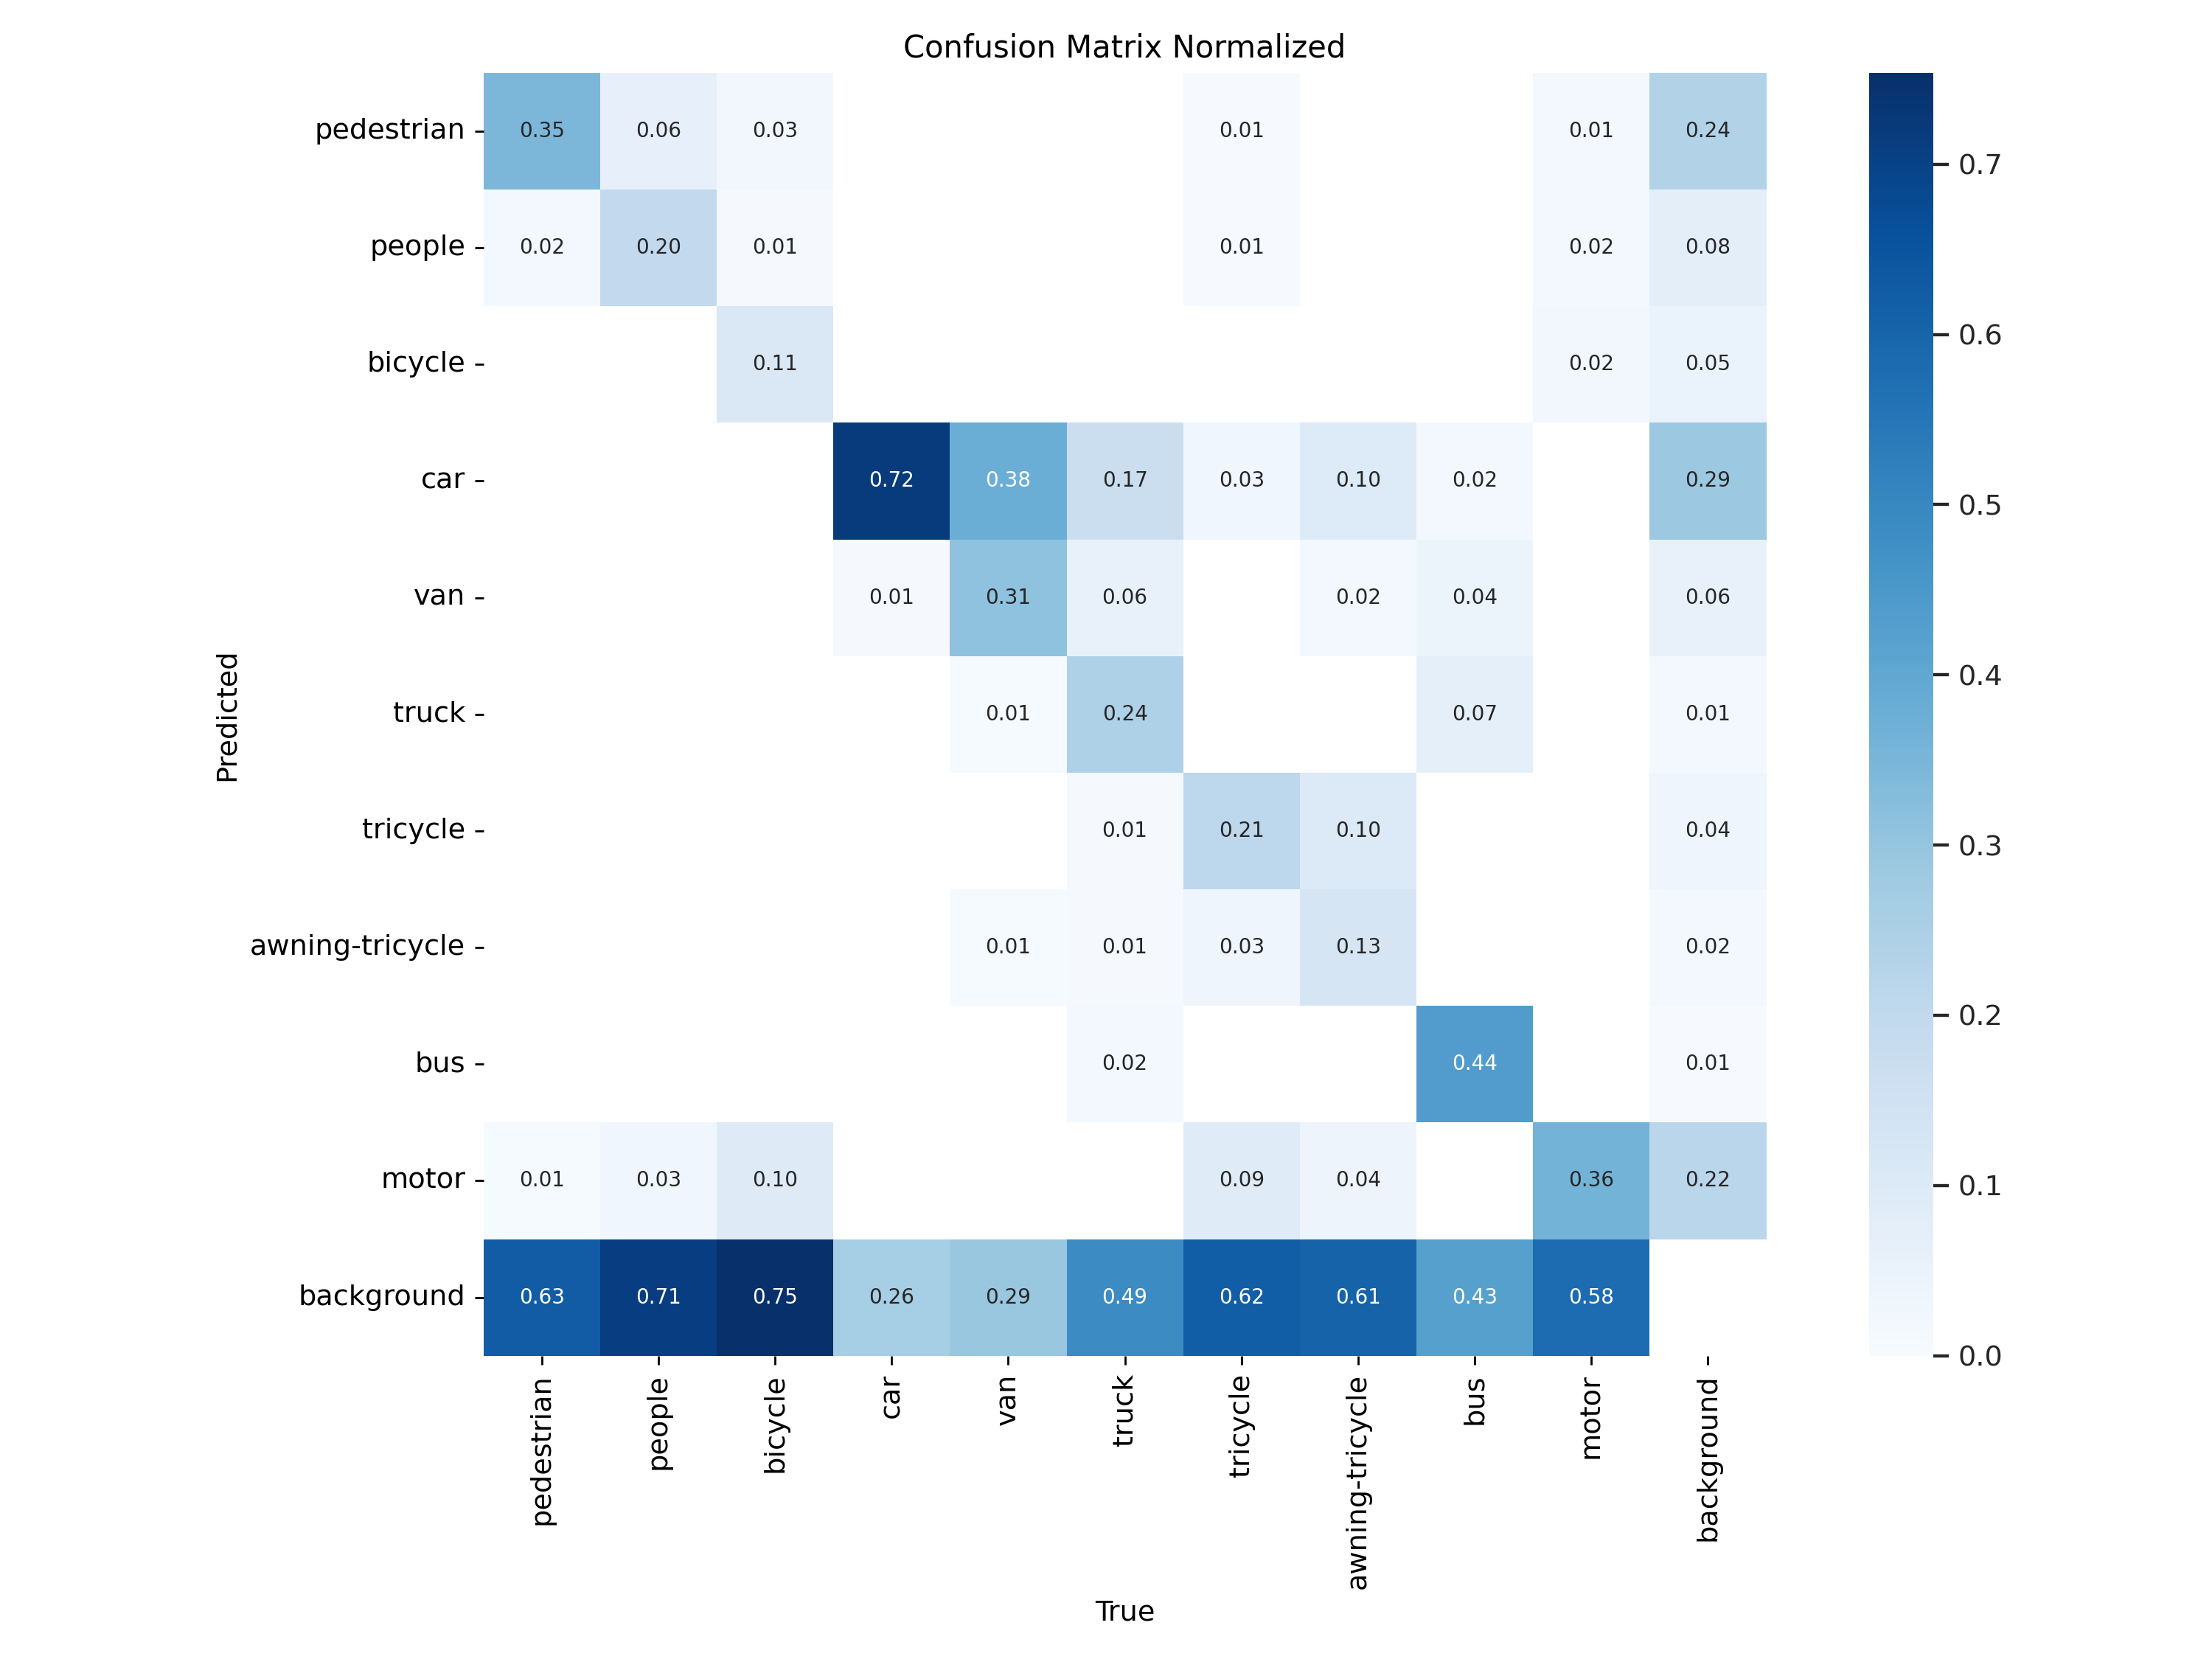
\includegraphics[width=0.4\textwidth]{../figure/vd_ex_confusion_matrix_normalized.png}
        }
        \subfloat[YOLOv11s\label{fig:vd_11s_cmn}]{
            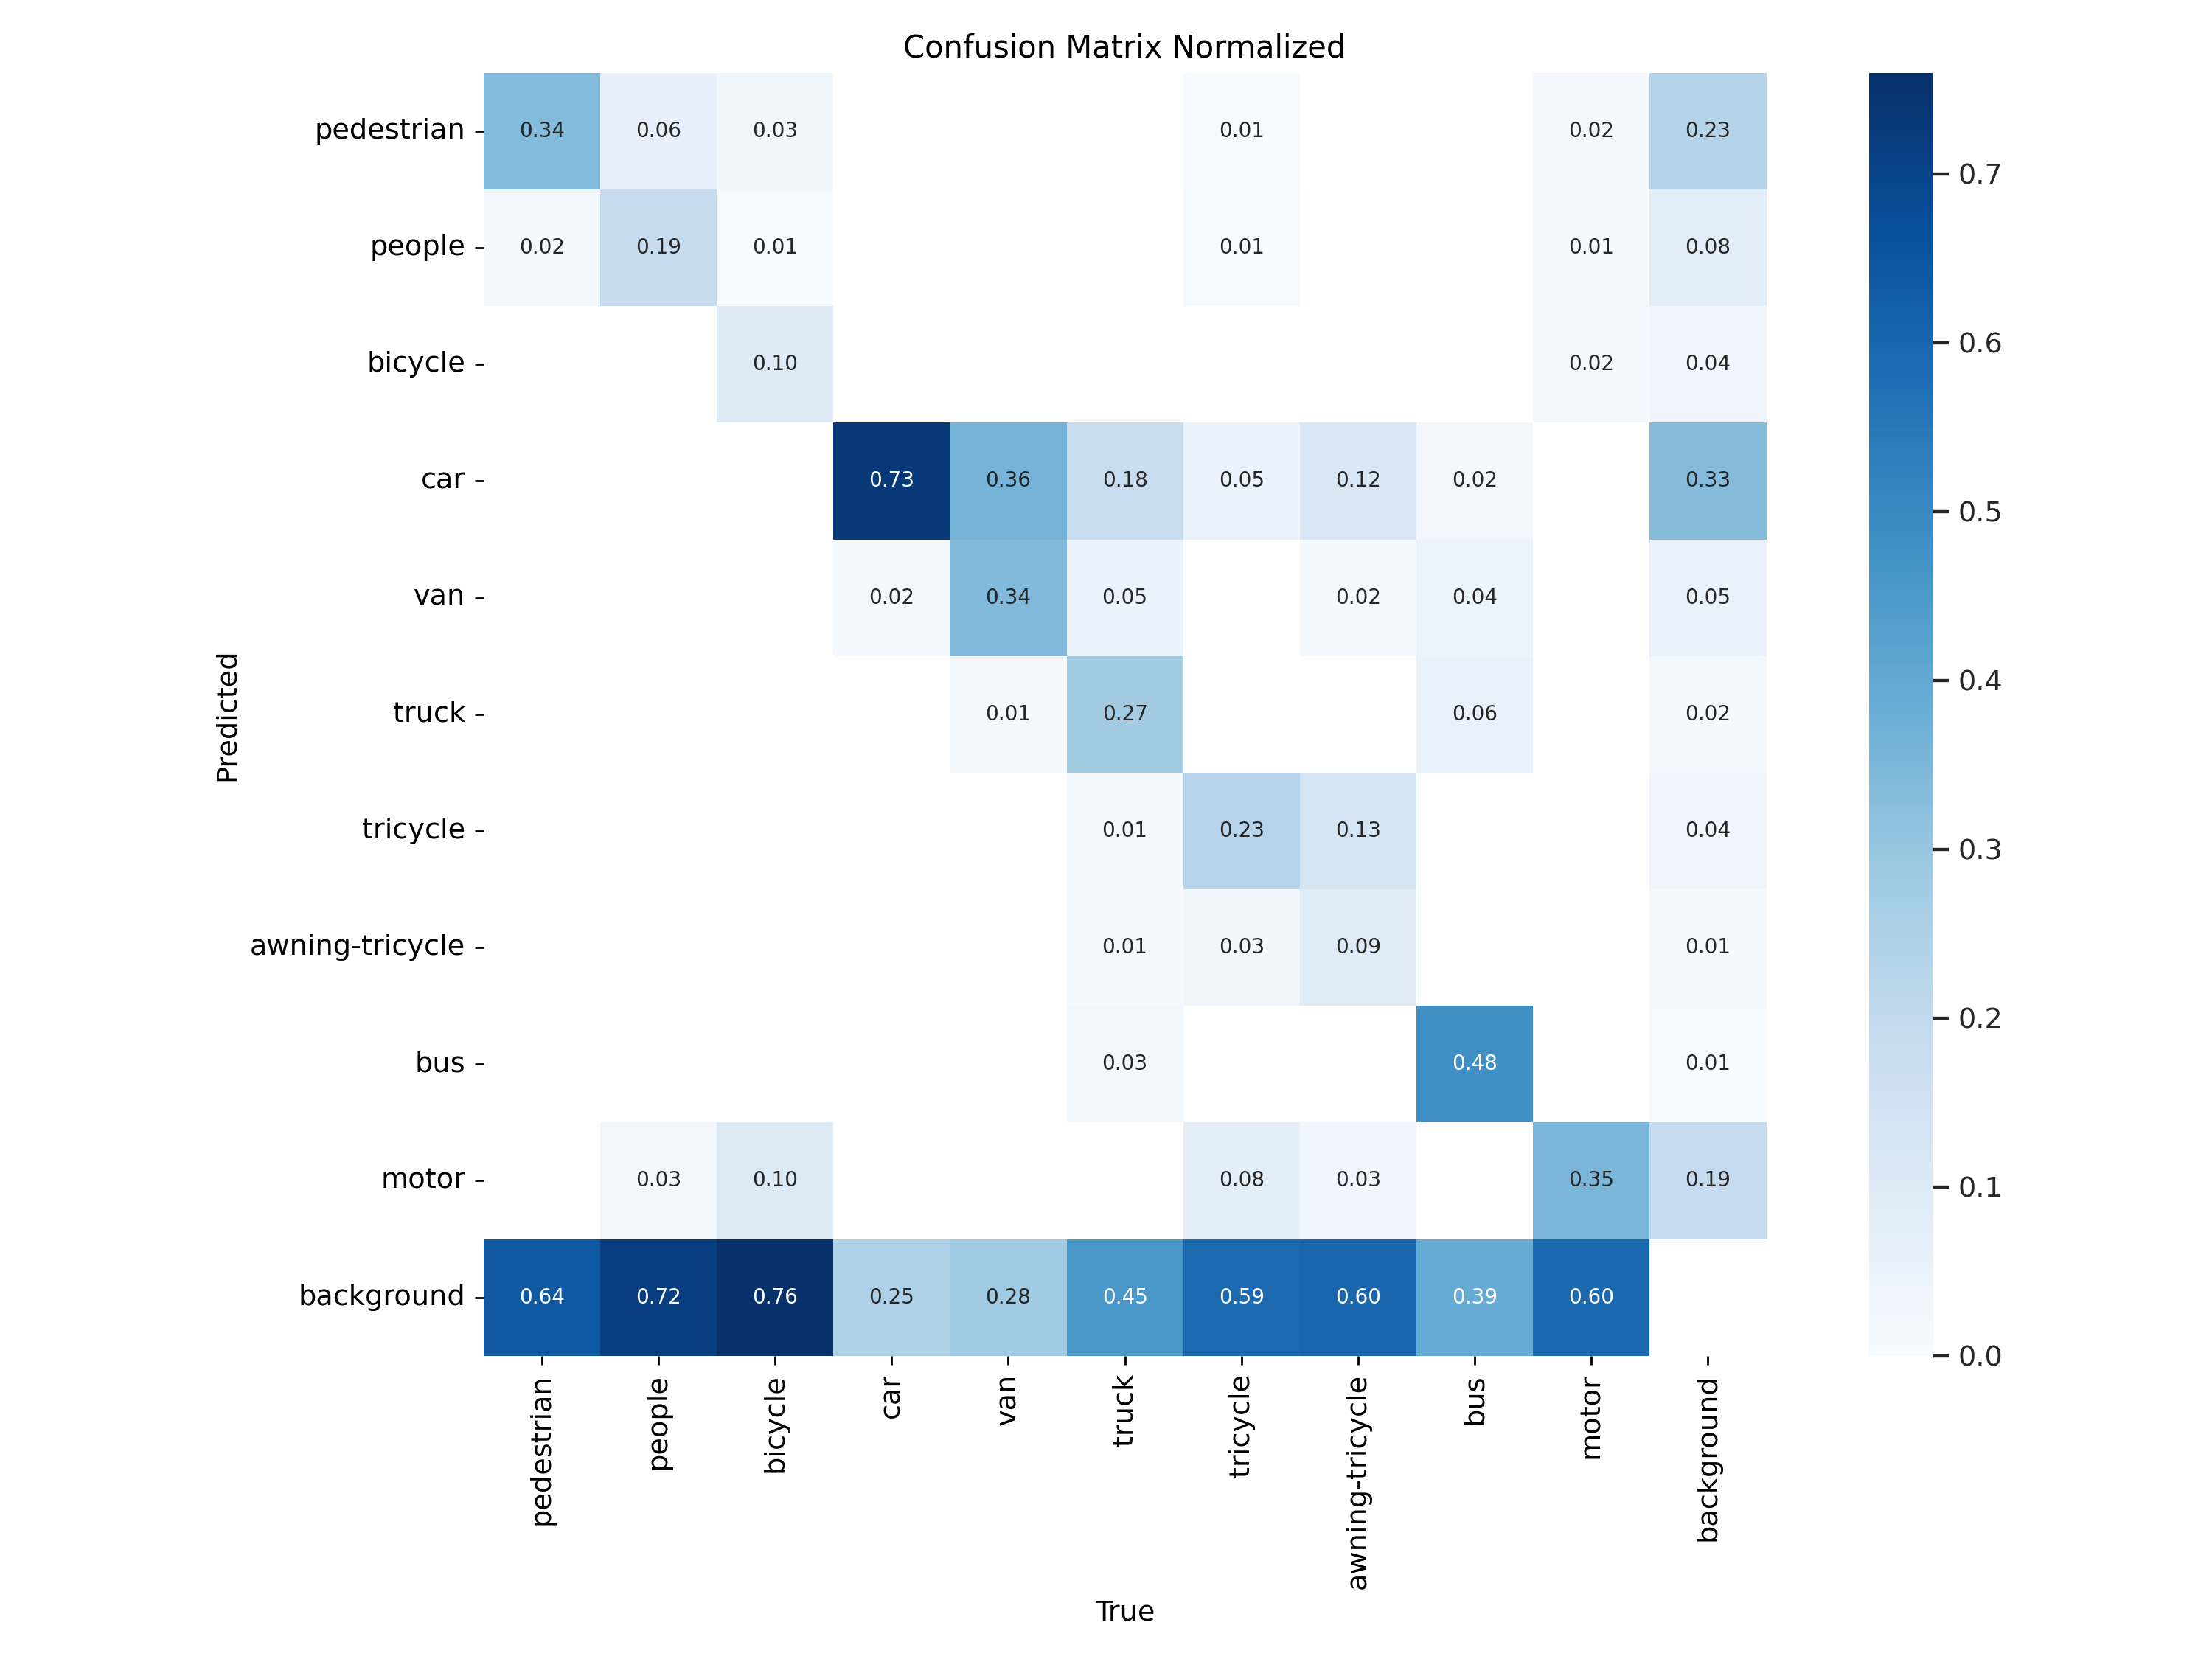
\includegraphics[width=0.4\textwidth]{../figure/vd_v11s_confusion_matrix_normalized.png}
        } \\
        \subfloat[YOLOv10s\label{fig:vd_10s_cmn}]{
            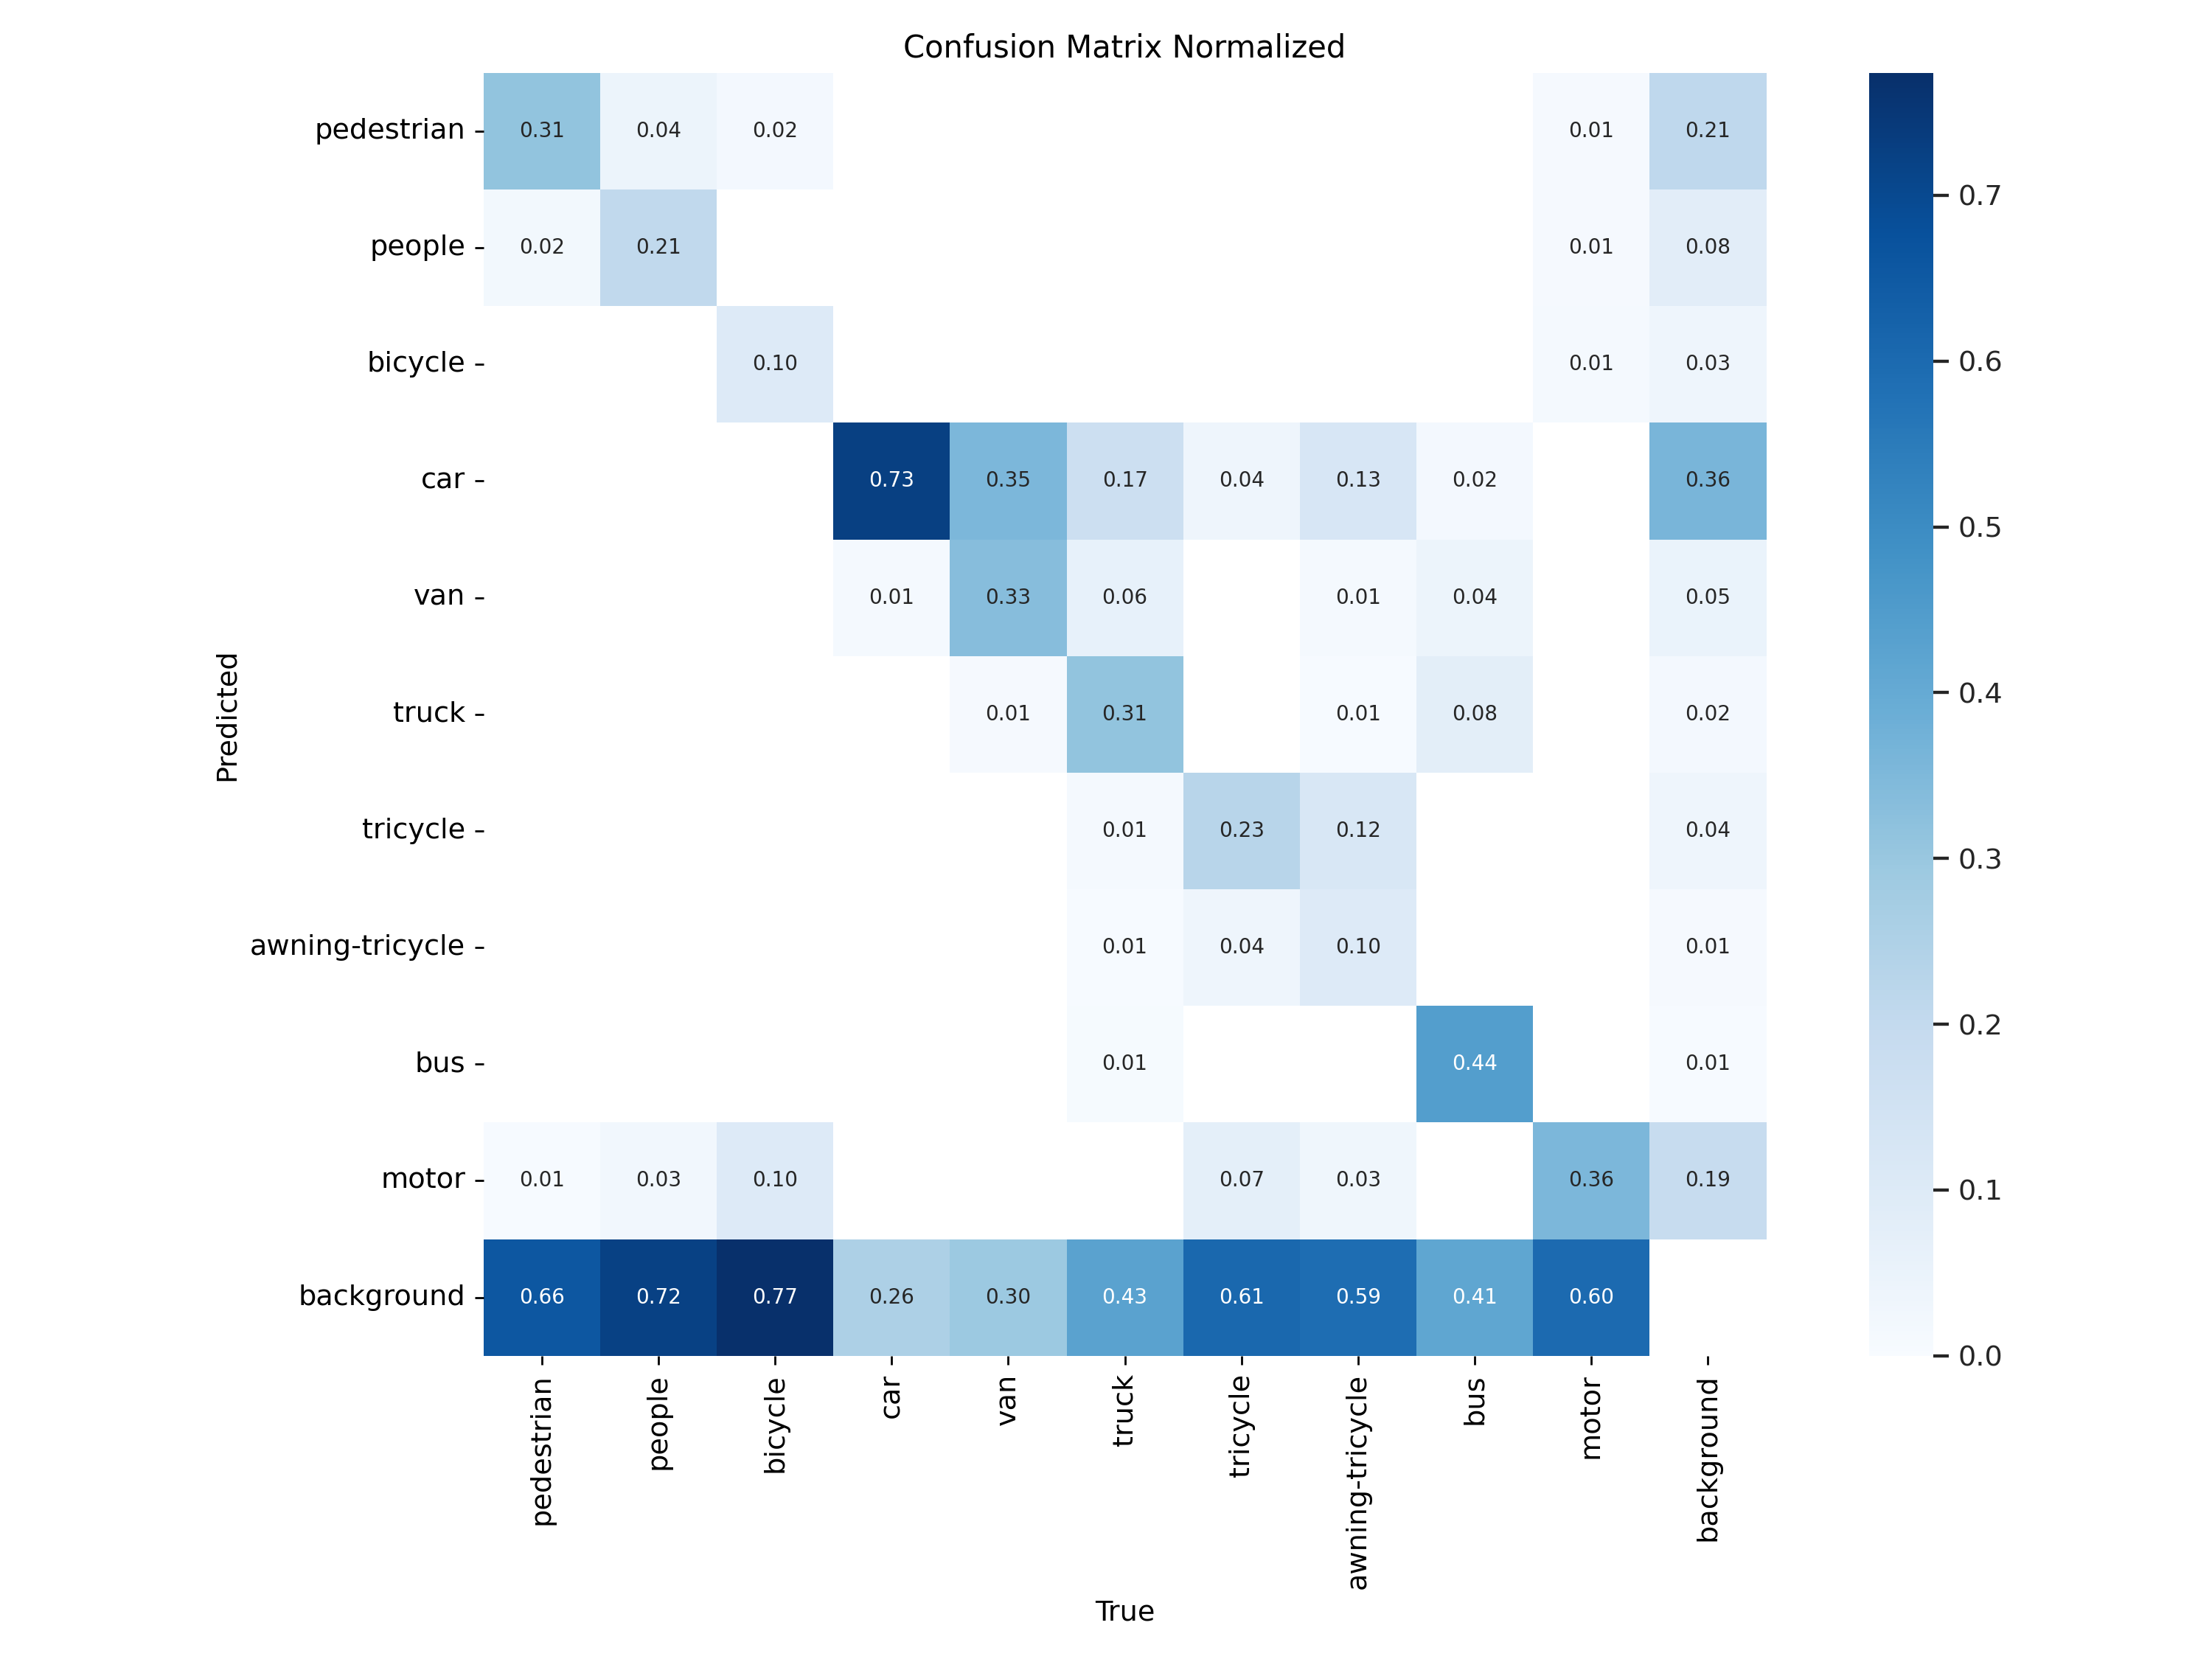
\includegraphics[width=0.4\textwidth]{../figure/vd_v10s_confusion_matrix_normalized.png}
        }
        \subfloat[YOLOv9s\label{fig:vd_9s_cmn}]{
            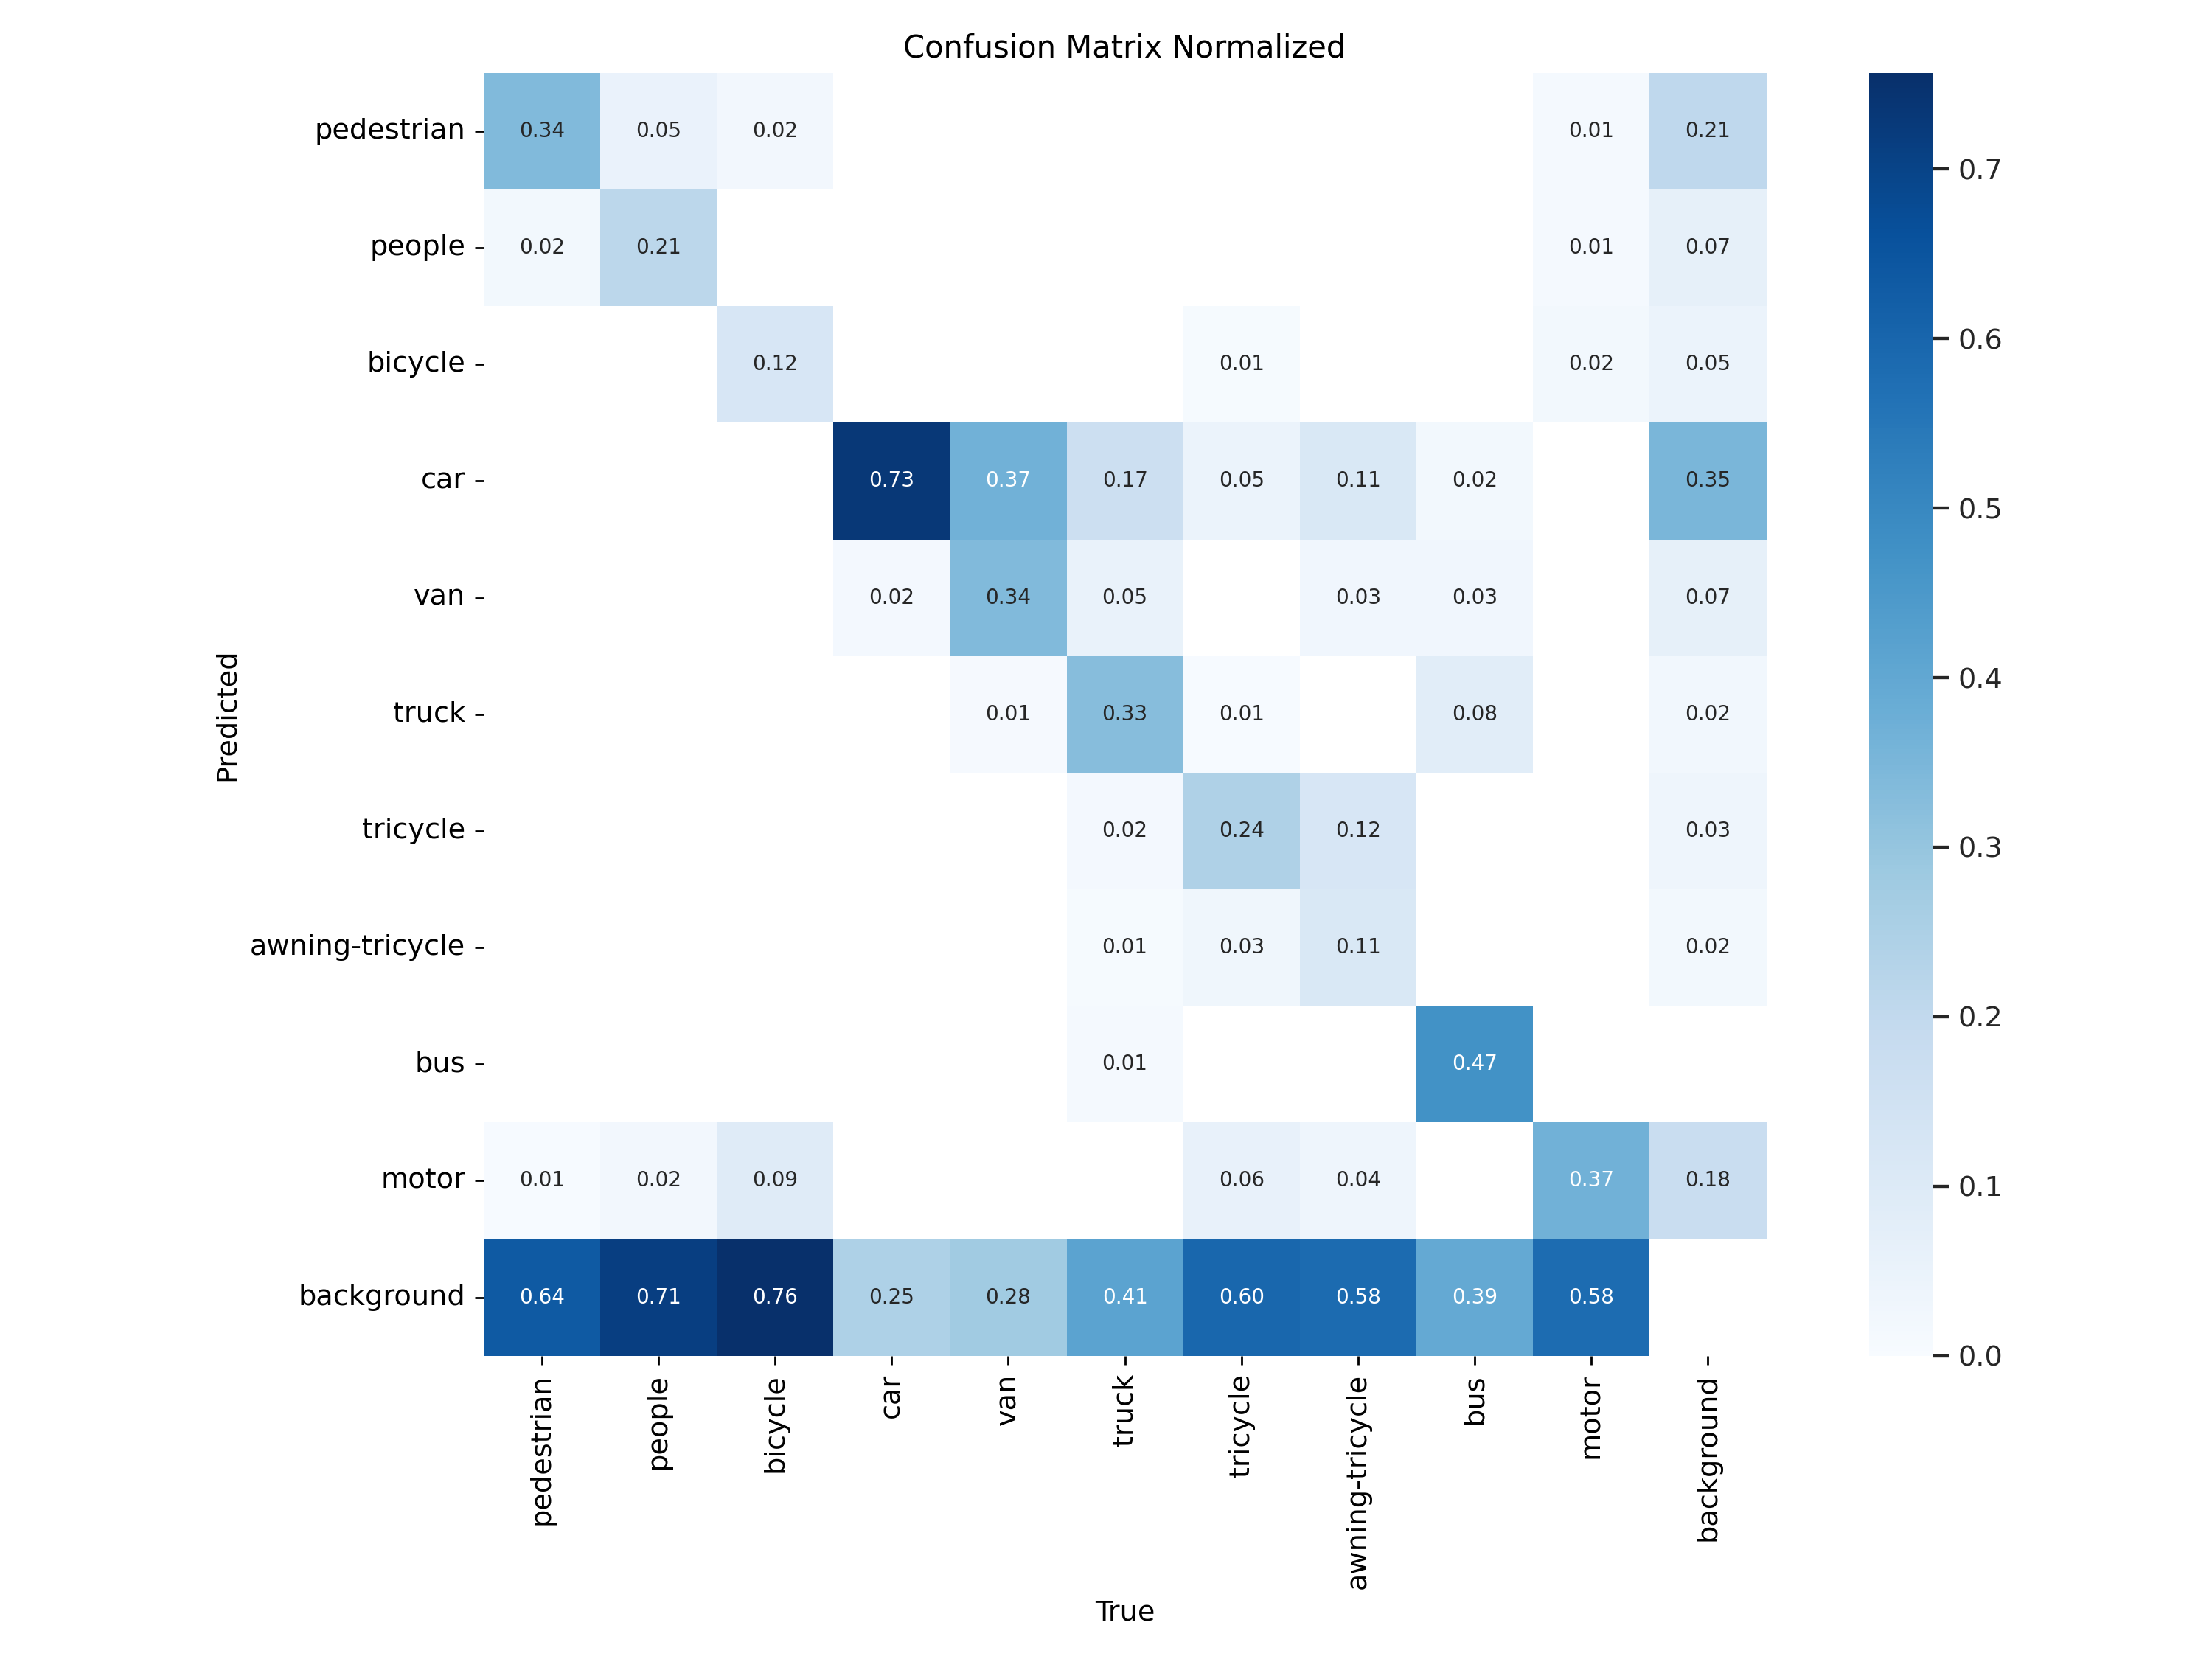
\includegraphics[width=0.4\textwidth]{../figure/vd_v9s_confusion_matrix_normalized.png}
        }
    \captionsetup{font=footnotesize}
    \bicaption{不同的网络模型在VisDrone数据集上的归一化混淆矩阵}{Symbol cross-reference table}
    \label{fig:vd_cmn}
\end{figure}

\begin{figure}[htbp]
    \centering
    \subfloat[EX-YOLO\label{fig:vd_ex_f1}]{
        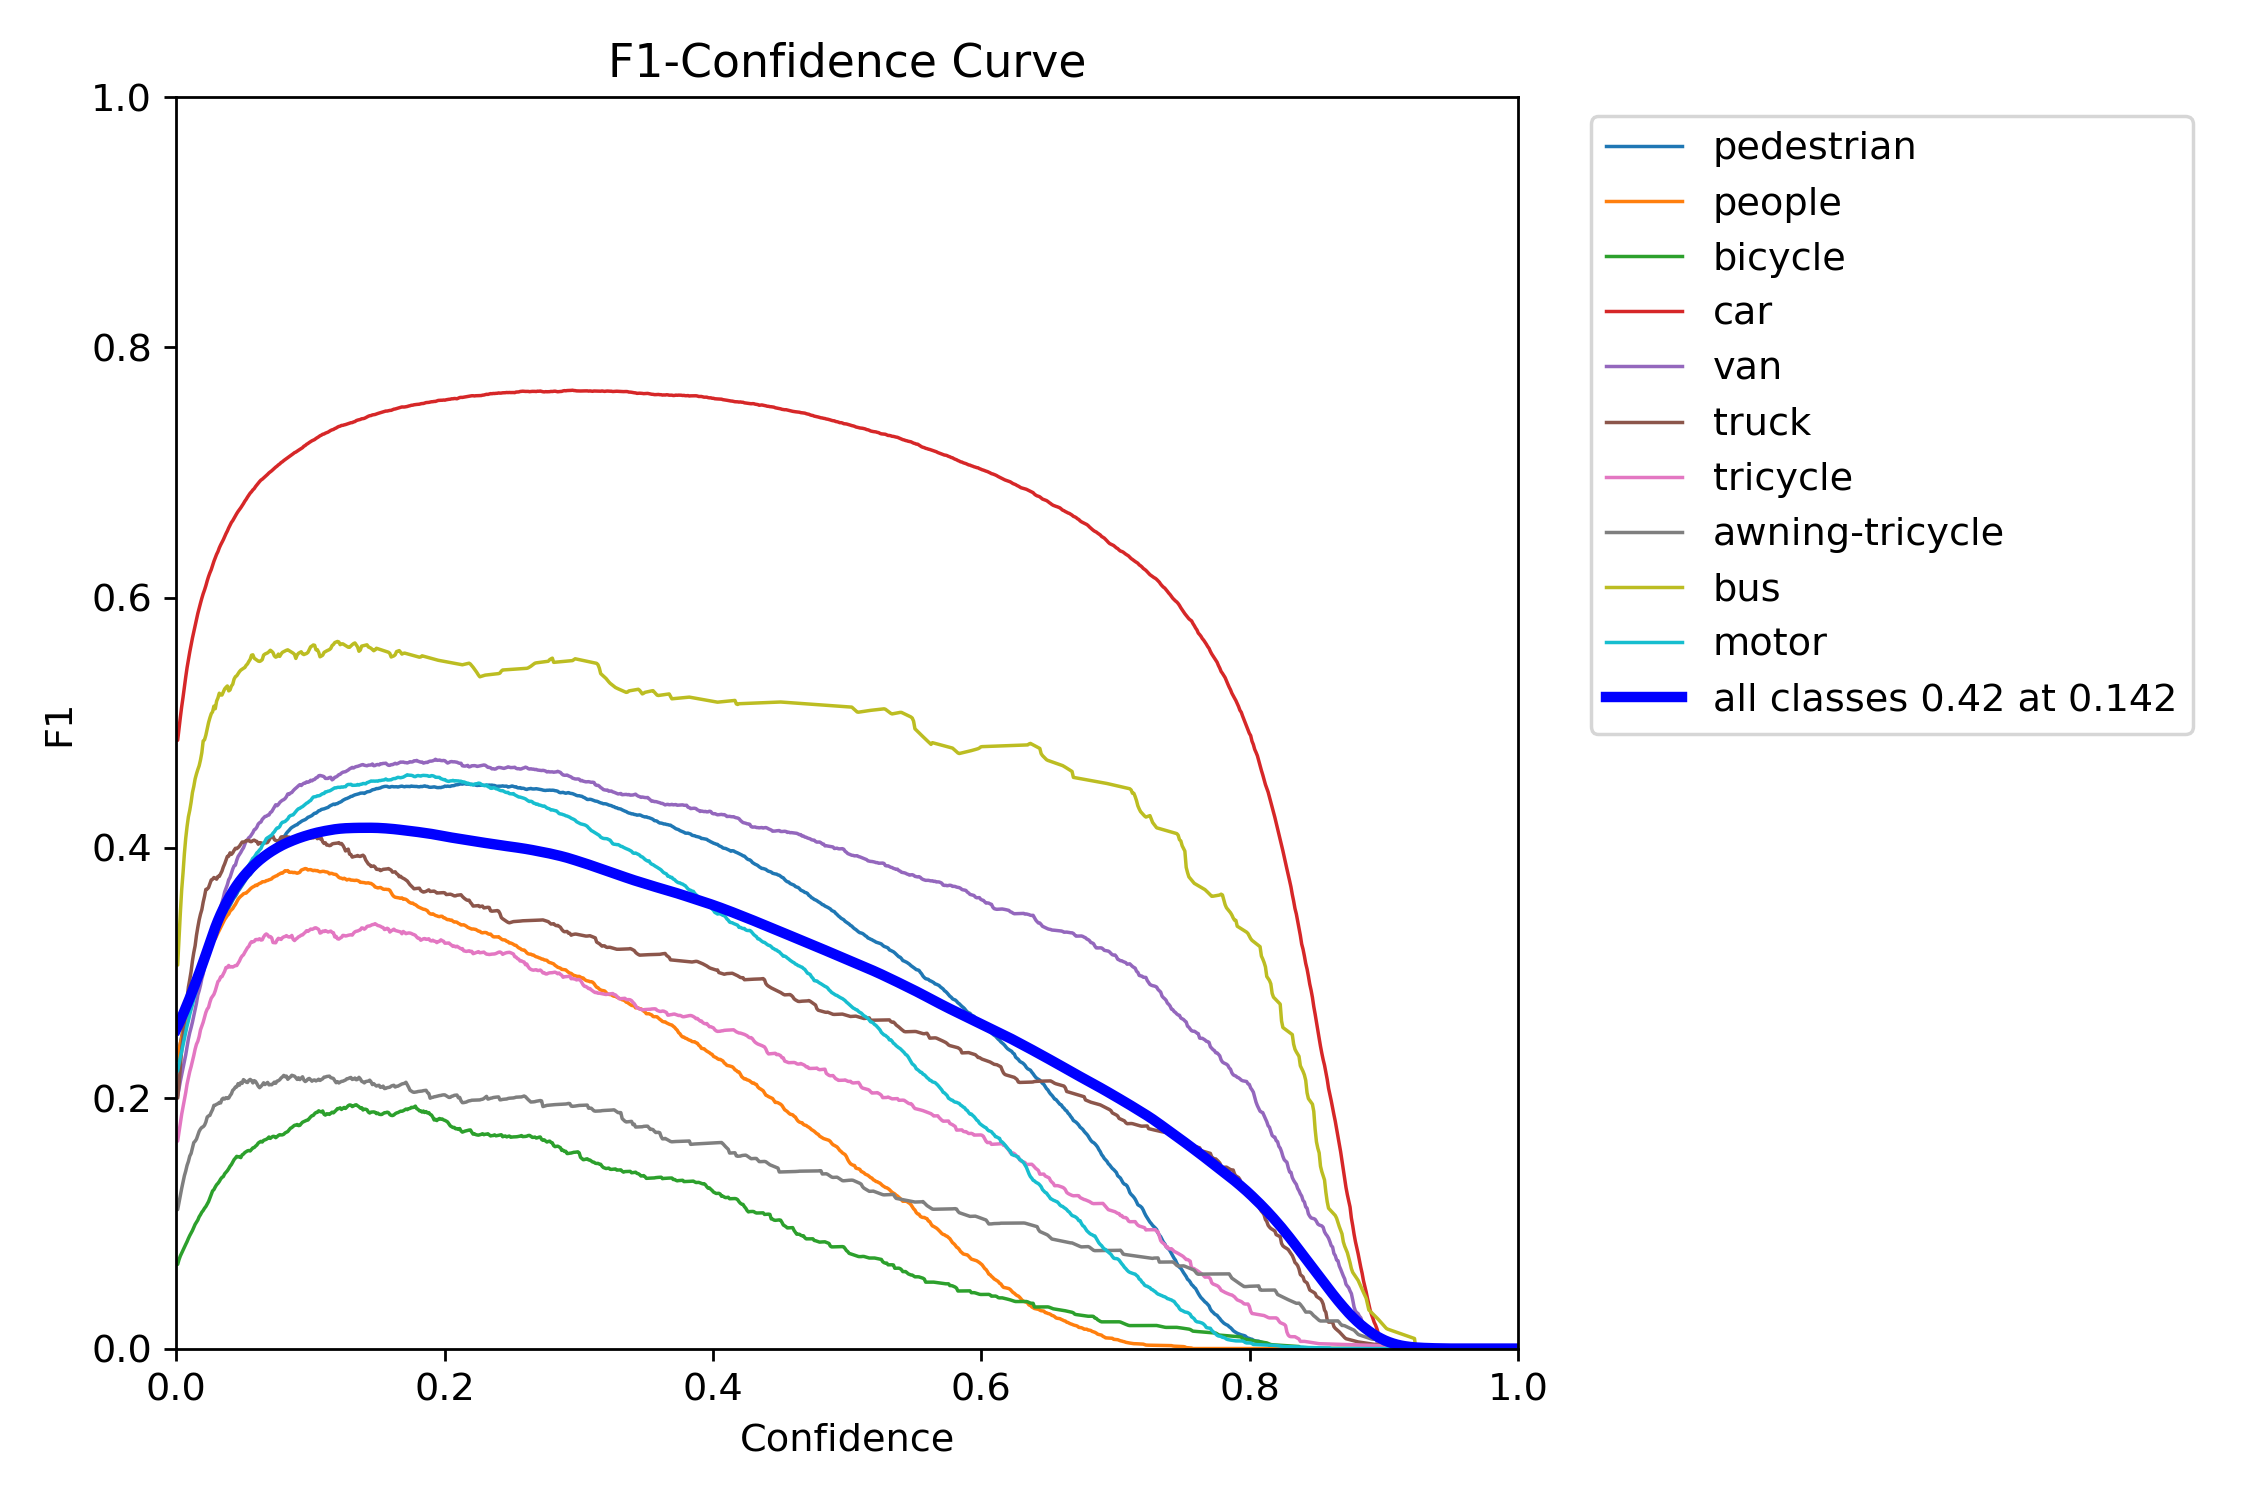
\includegraphics[width=0.4\textwidth]{../figure/vd_ex_F1_curve.png}
    }
    \subfloat[YOLOv11s\label{fig:vd_11s_f1}]{
        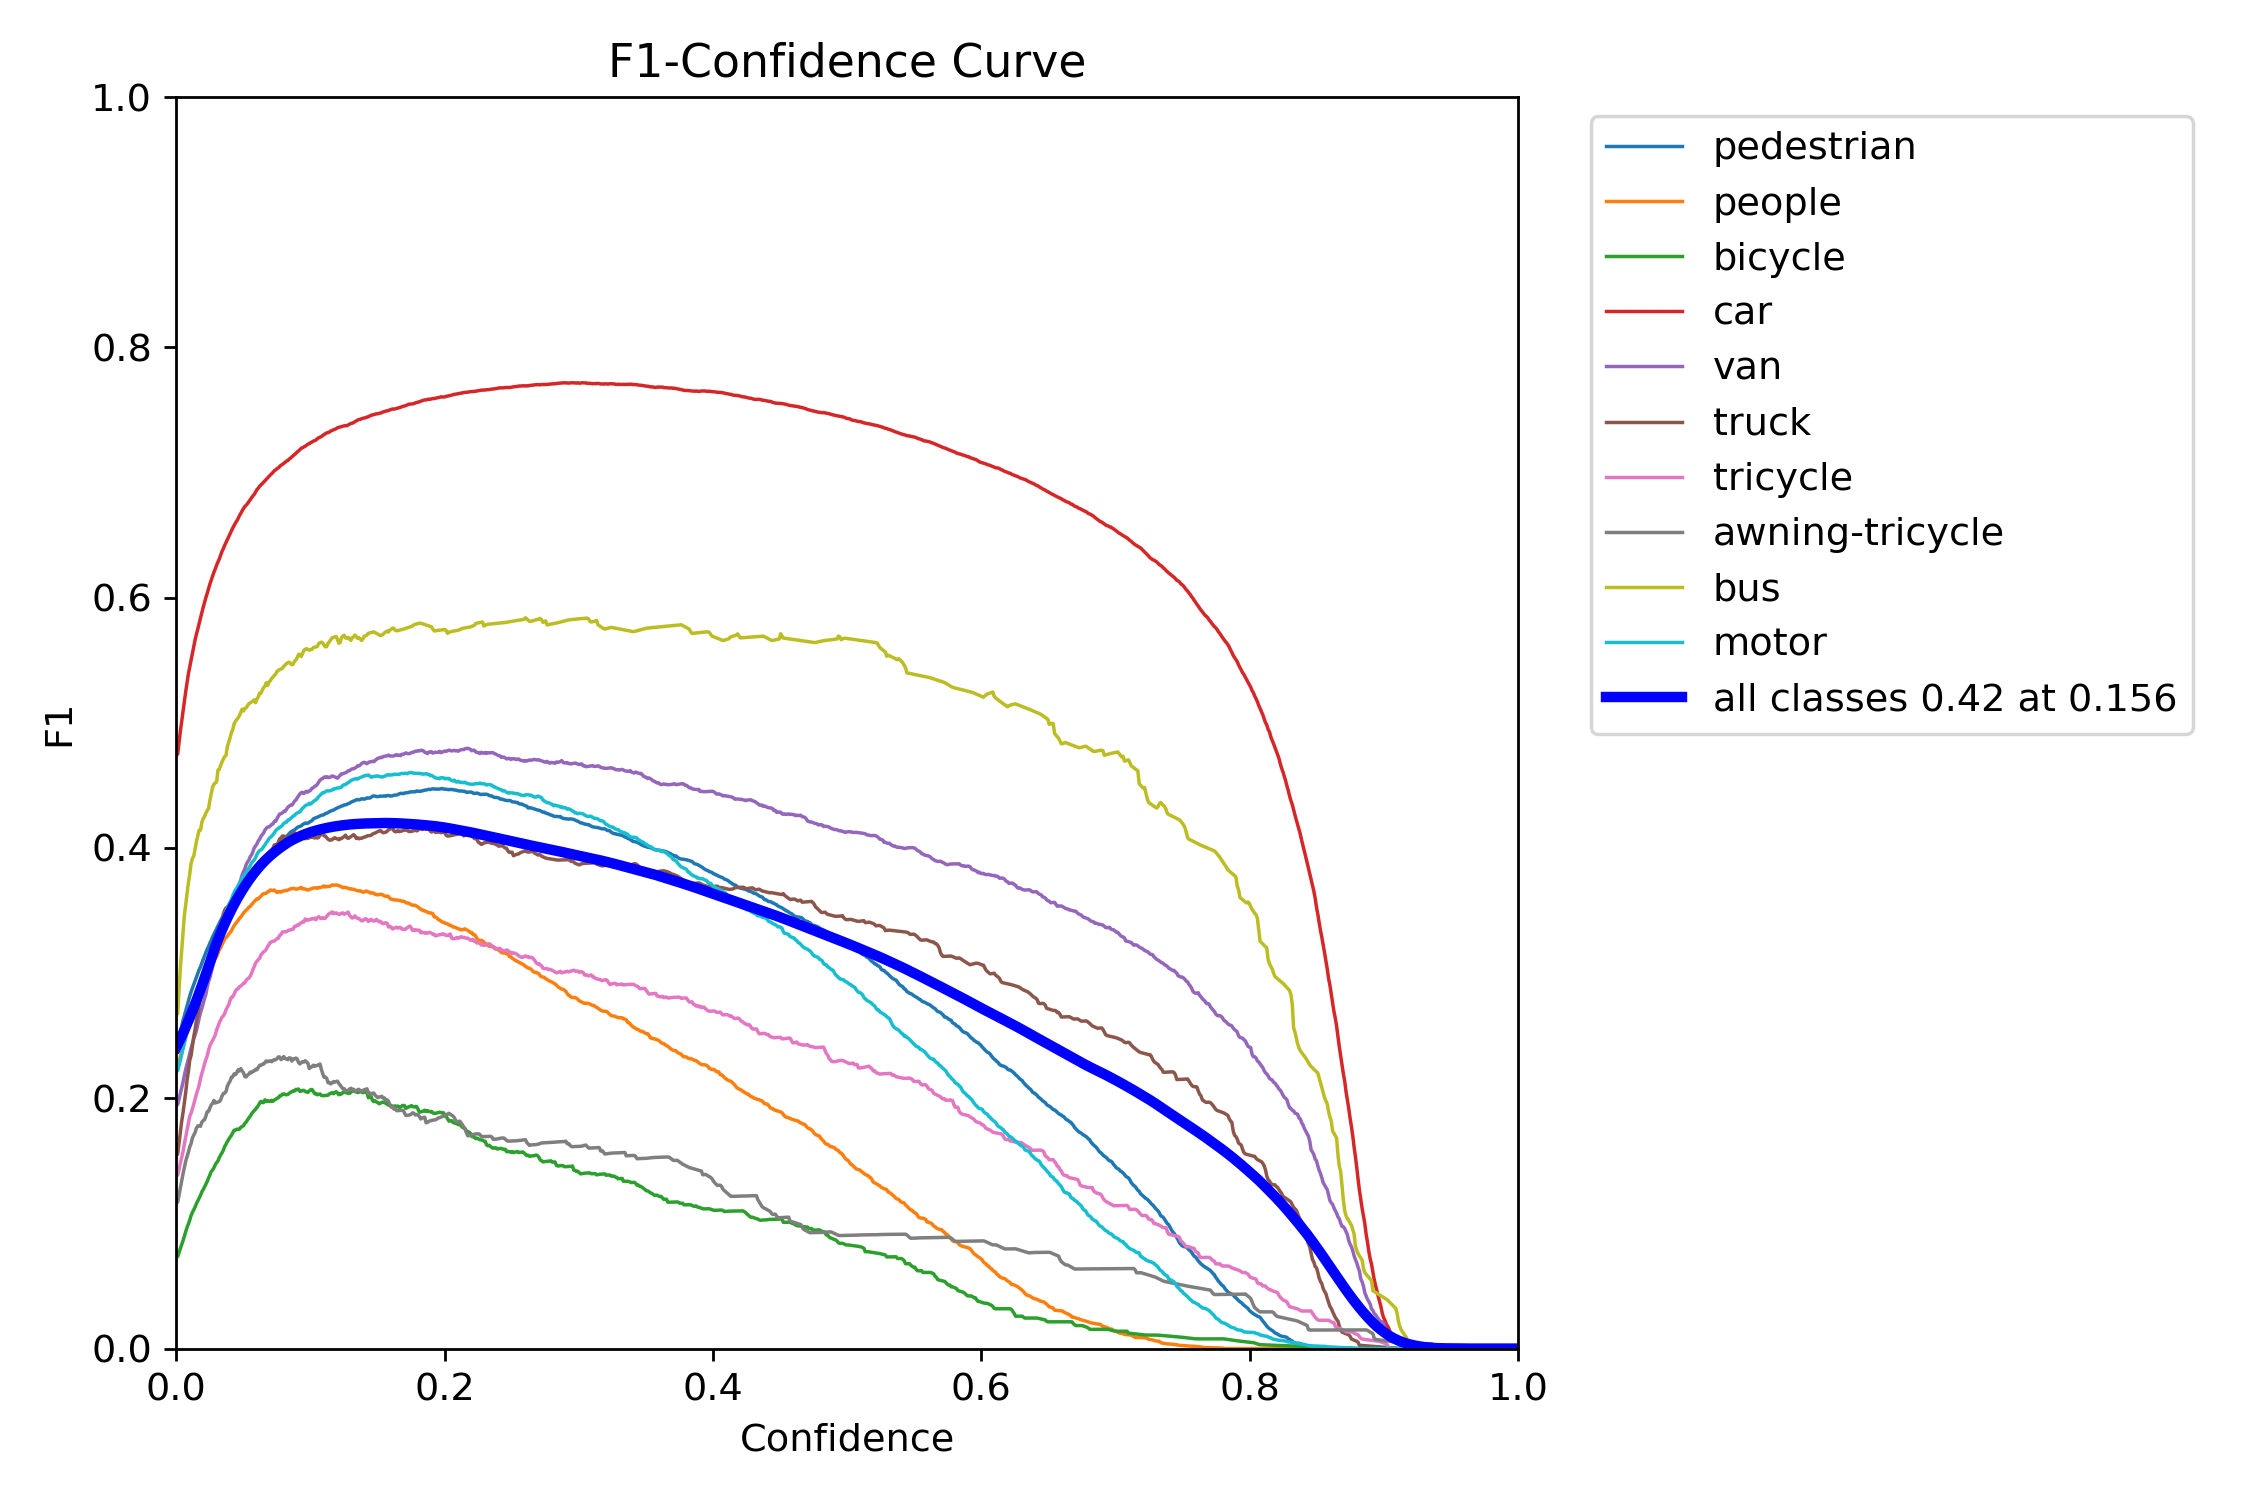
\includegraphics[width=0.4\textwidth]{../figure/vd_v11s_F1_curve.png}
    } \\
    \subfloat[YOLOv10s\label{fig:vd_10s_f1}]{
        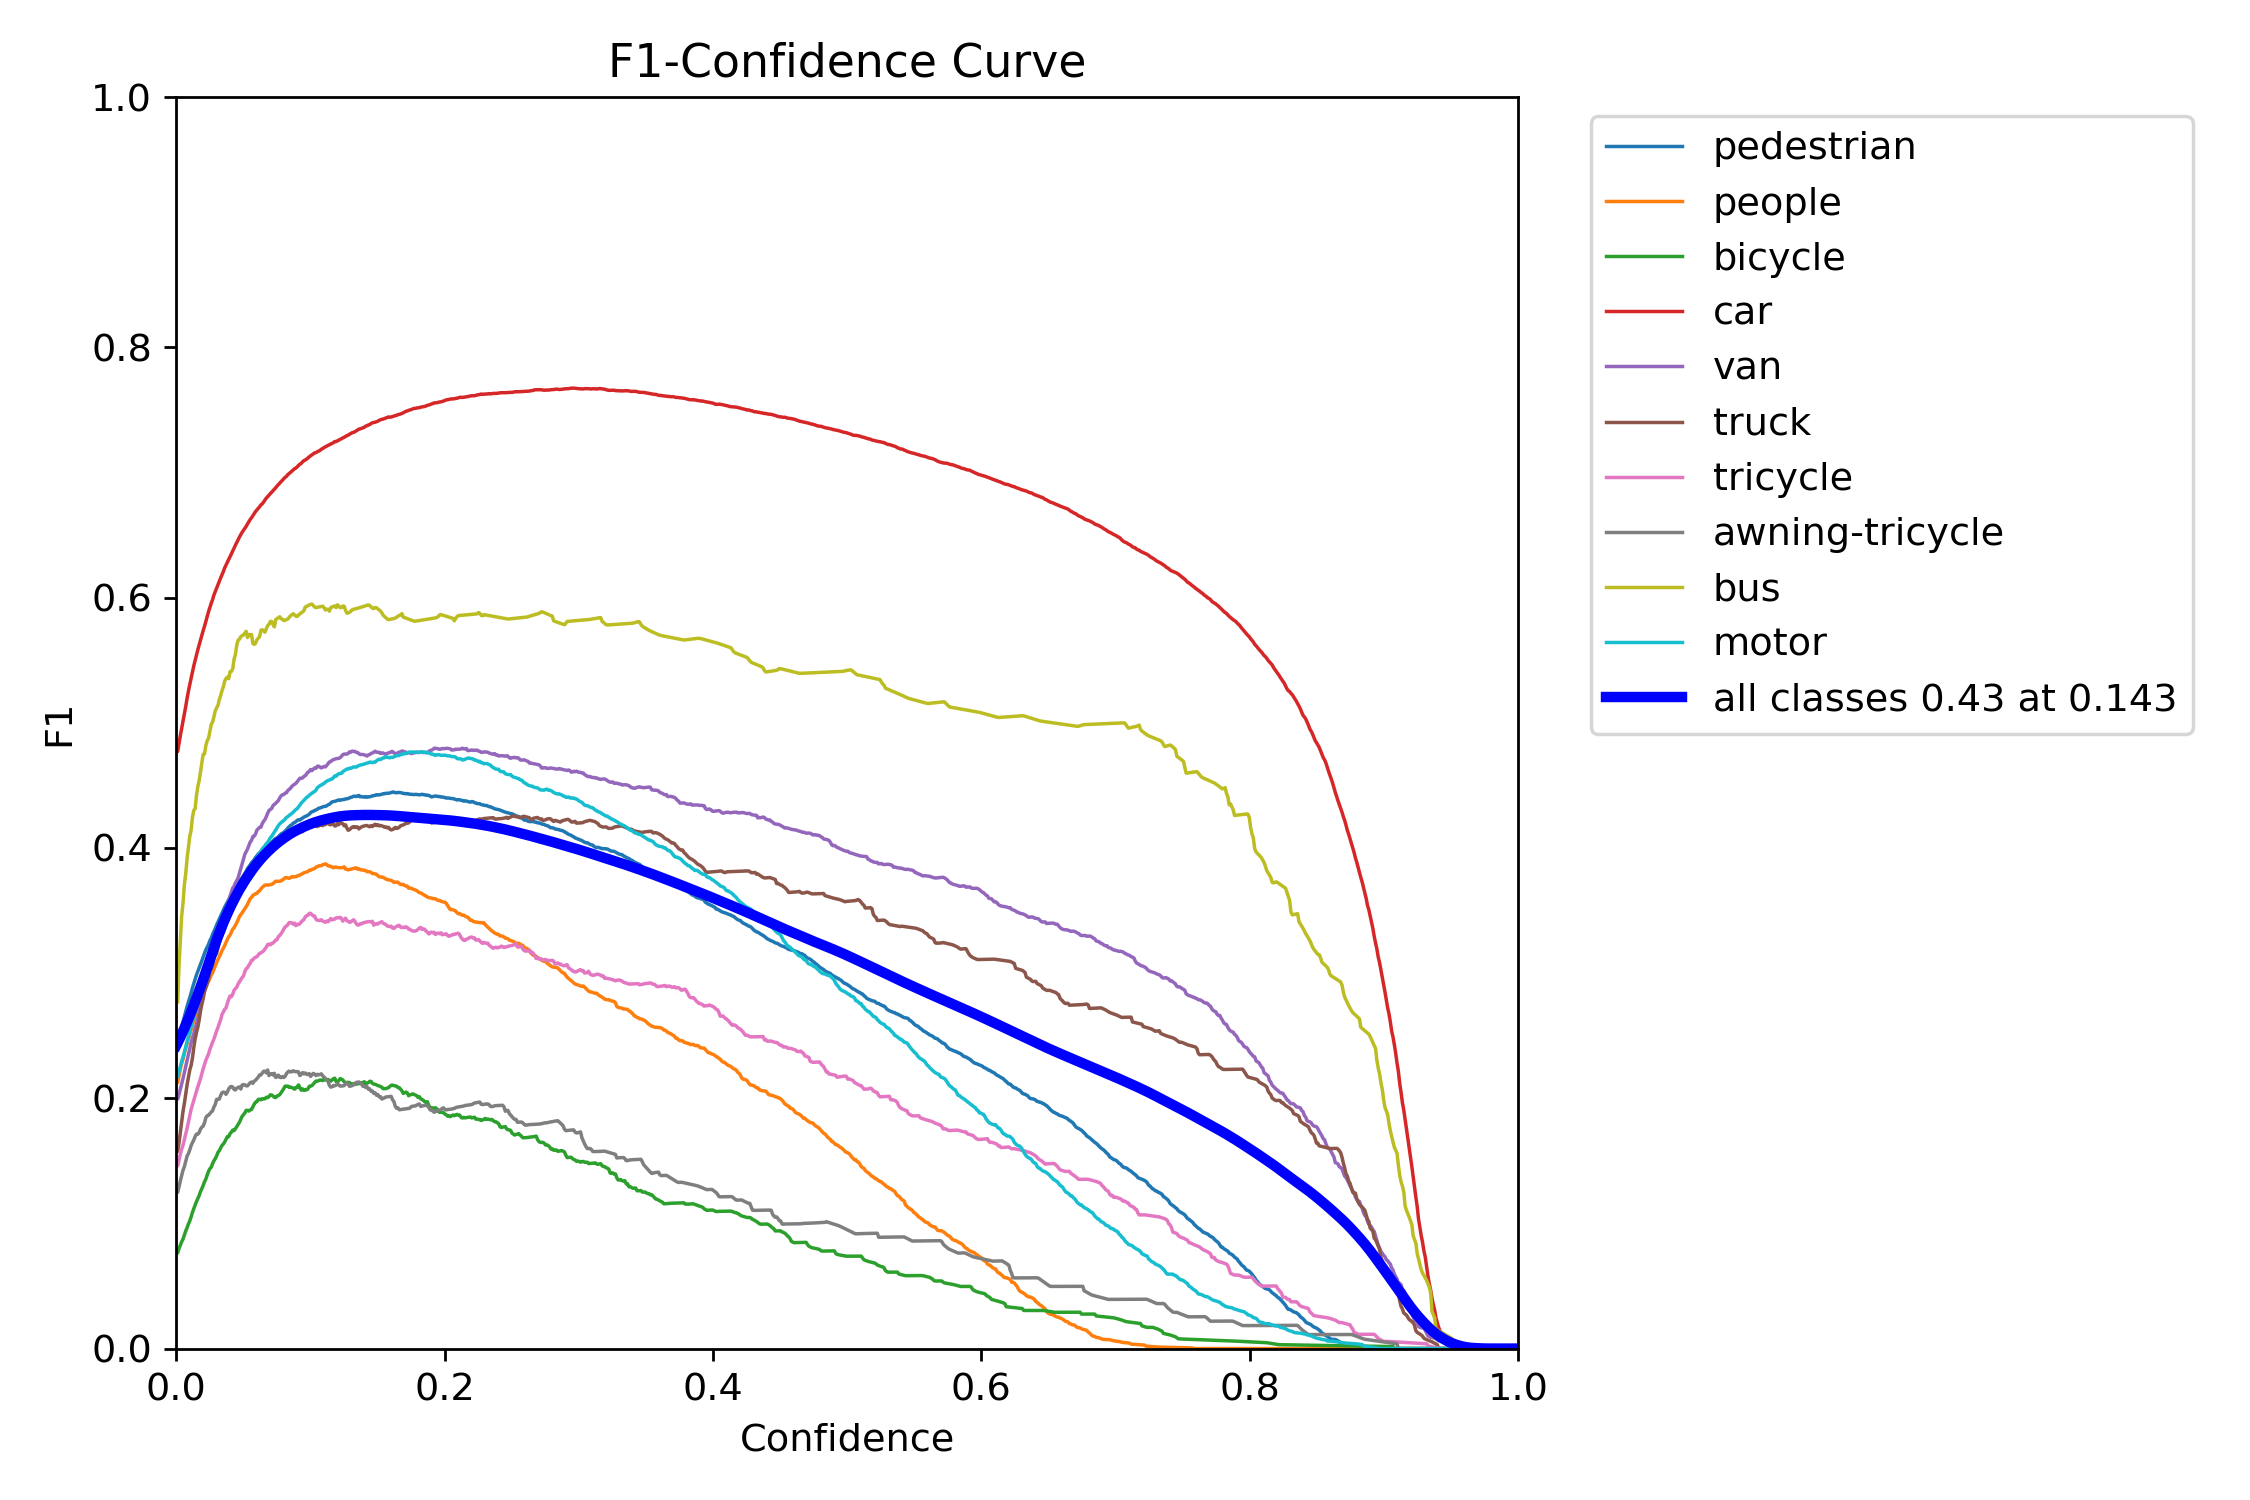
\includegraphics[width=0.4\textwidth]{../figure/vd_v10s_F1_curve.png}
    }
    \subfloat[YOLOv9s\label{fig:vd_9s_f1}]{
        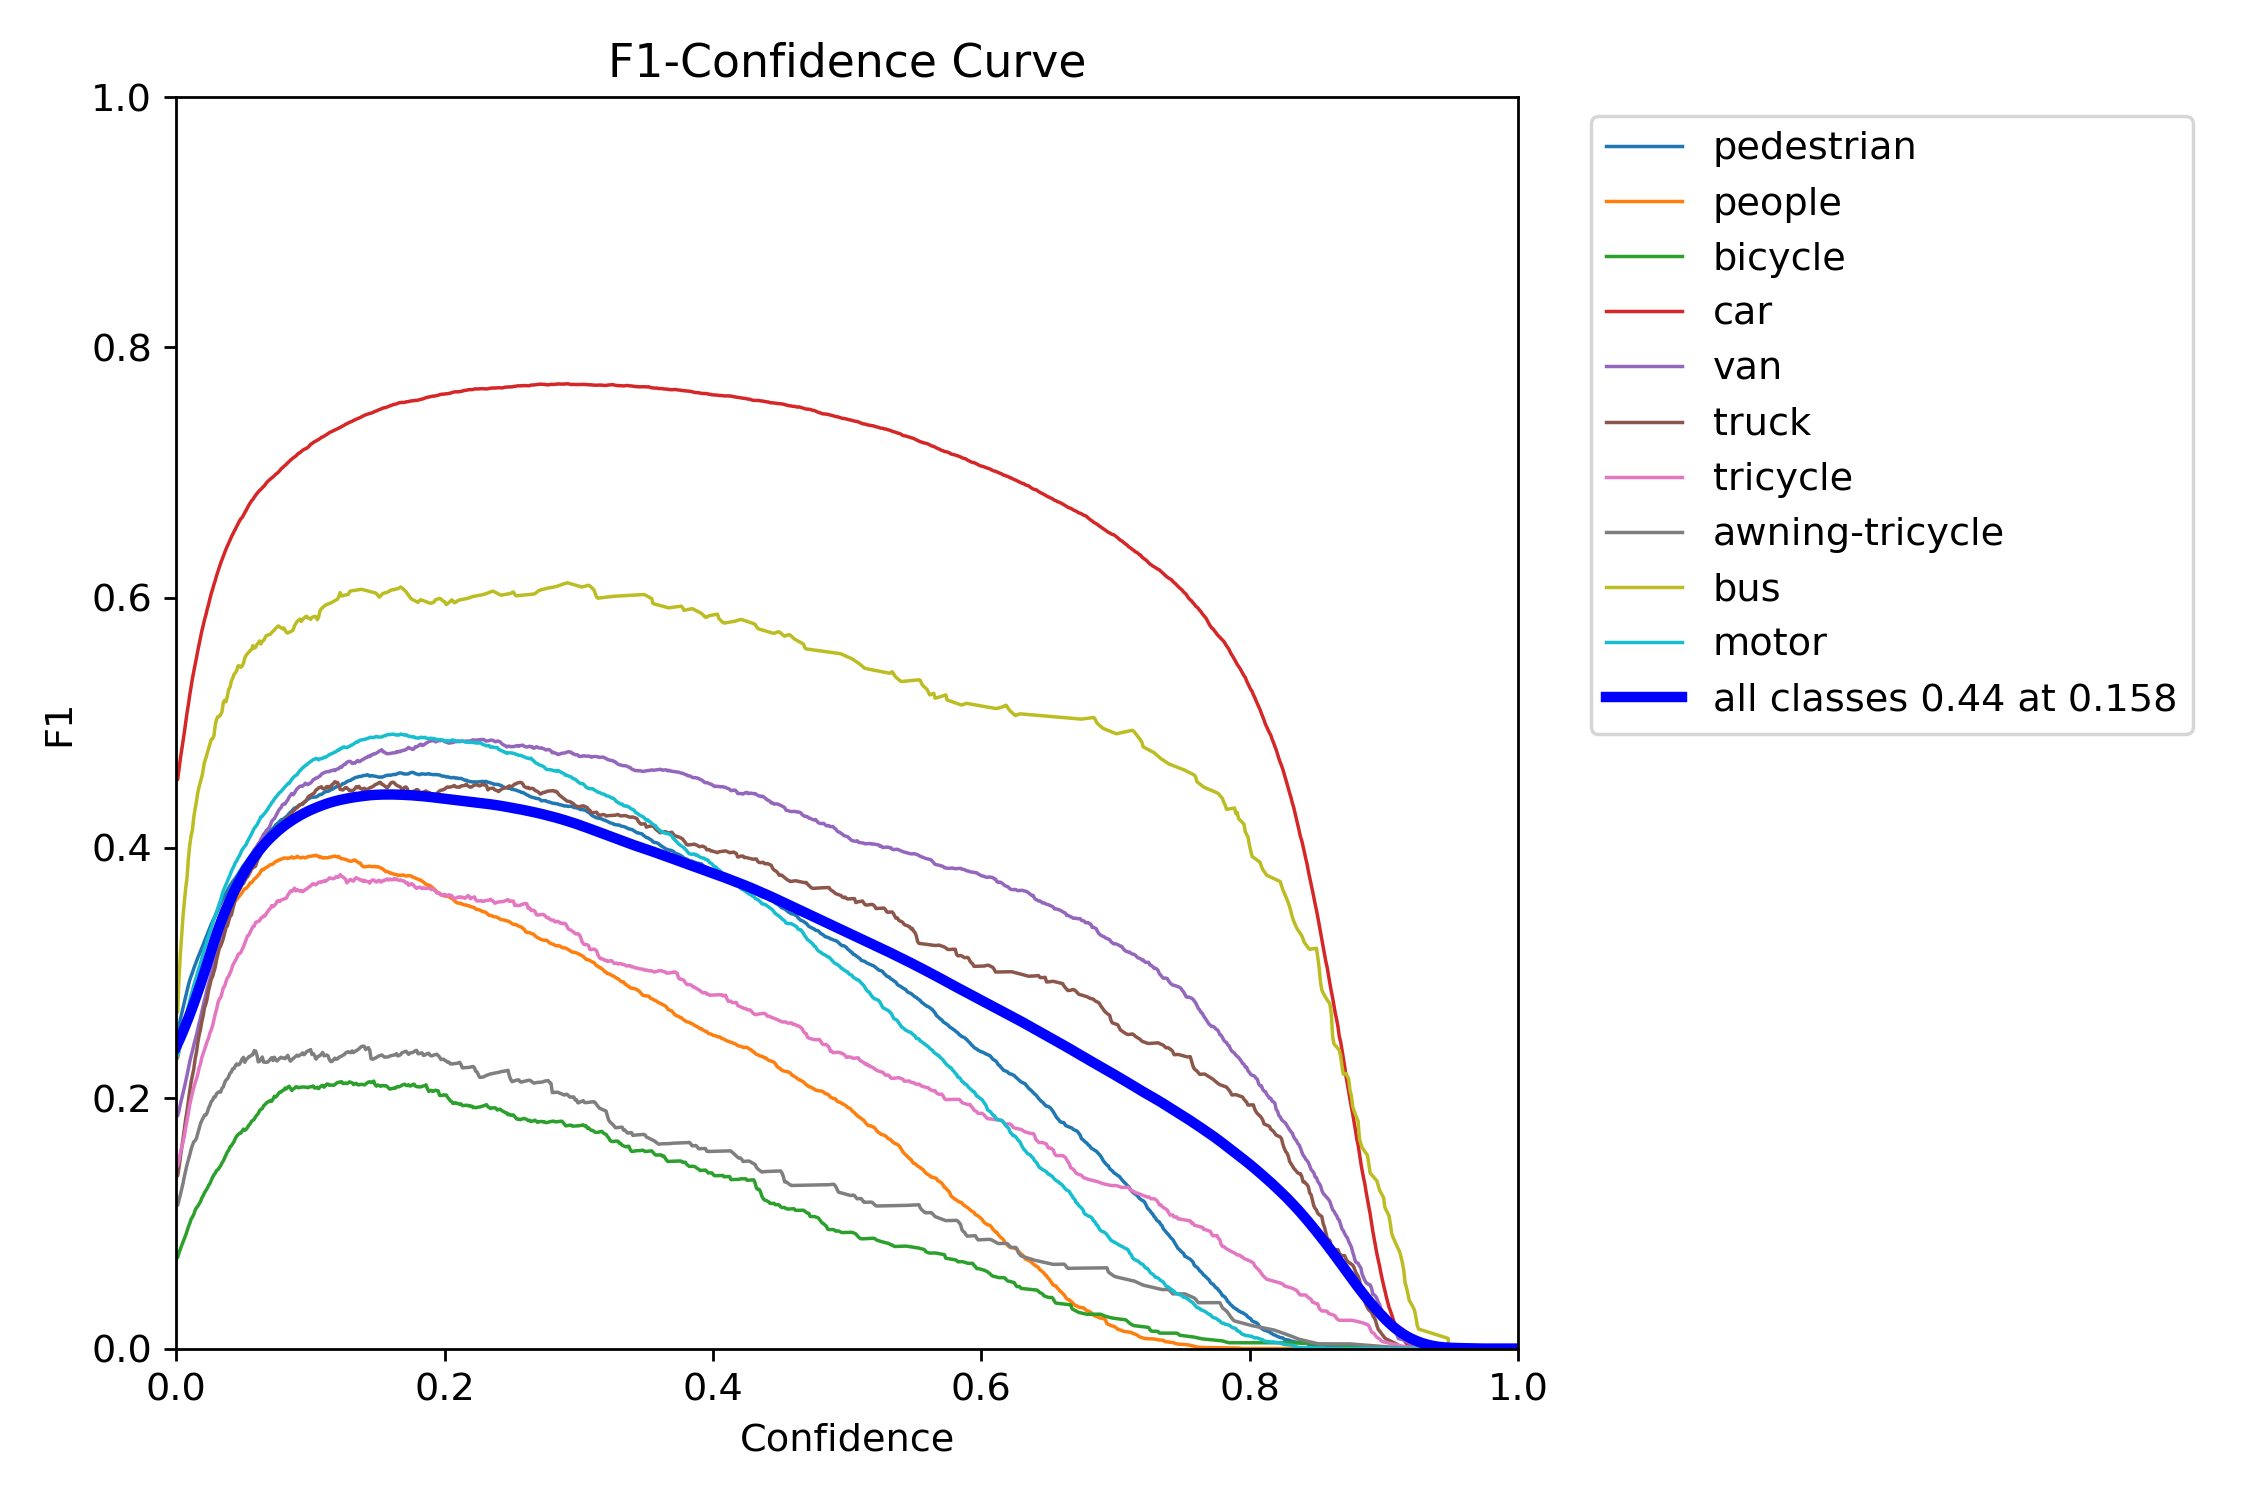
\includegraphics[width=0.4\textwidth]{../figure/vd_v9s_F1_curve.png}
    }
    \captionsetup{font=footnotesize}
    \bicaption{不同的网络模型在VidDrone数据集上的F1得分}{Symbol cross-reference table}
    \label{fig:vd_f1}
\end{figure}

在表 \ref{tab:compare_studies_vd} 中,就计算量(GFLOPs)而言,our 模型明显低于其他值为15.4的比较模型。 YOLOv11s是21.3,YOLOv10s是24.5,YOLOv9s高达26.7。 这一结果充分表明,改进后的算法在减少计算量方面取得了出色的效果。 较低的计算量有助于延长无人机的耐用性,并提高其在复杂环境中的运行效率,使其能够更快地处理图像数据并做出准确的判断。

在精度(P)方面,our 模型是0.514,高于YOLOv11s的0.485和YOLOv10s的0.501,略低于YOLOv9s的0.525。 在召回(R)方面,our 模型是0.372,略低于YOLOv11s的0.381和YOLOv10s的0.380,与YOLOv9的0.392相比存在一定的差距。

图 \ref{fig:vd_cmn} 展示了 YOLOv9s、YOLOv10s、YOLOv11s 以及 our 模型在 VisDrone 数据集针对不同类别目标的预测状况,以归一化混淆矩阵热力图形式呈现。热力图颜色深浅与预测概率正相关,颜色愈深表示预测准确率愈高,颜色愈浅则表明预测准确率较低。对角线数据反映模型成功预测正确标签的情况,非对角线数据则体现模型标签预测错误的情形。

从图 \ref{fig:vd_ex_cmn} 至图 \ref{fig:vd_9s_cmn} 可见,各模型在不同类别上的预测表现存在差异。
综合归一化混淆矩阵热力图信息可知,在 VisDrone 数据集上,YOLOv9s 模型在预测正确类别方面表现较为出色,这一结论与表 \ref{tab:compare_studies_vd} 中的数据相呼应 —— YOLOv9s 的精确度(0.525)和召回率(0.392)均处于较高水平。our 模型的精确度(0.514)略低于 YOLOv9s,但召回率(0.372)与 YOLOv11s(召回率 0.381)和 YOLOv10s(召回率 0.380)相近,整体性能优于 YOLOv10s 模型。尽管 our 模型在精确度和召回率上未超越 YOLOv9s,但其在特定类别预测上展现出独特优势,例如在 “pedestrian” 和 “awning-tricycle”类别预测中,our 模型的准确率达到了 0.35 和 0.13,相较于其他模型具有一定的竞争力。
总体而言,our 模型在 VisDrone 数据集上的表现与 YOLO 系列模型各有优劣。虽然在精确度和召回率上略逊于 YOLOv9s,但在部分类别预测上展现出独特优势,且整体性能优于 YOLOv10s 模型,与 YOLOv11s 模型相近,具有进一步优化和提升的潜力。

从$mAP_{0.5}$的主要性能指数来看,our 模型达到了0.390,与YOLOv10s相同,高于YOLOv11s的0.383,略低于YOLOv9s的0.402。 虽然YOLOv9s的mAP最高,但其计算量也是最大的,这在一定程度上限制了其在实际应用中的可行性。 相比之下,our 模型仍然保持高mAP,同时有效减少计算量,这反映了改进算法在提高检测精度方面的优势。 在无人机的小目标检测任务中,关键是准确识别各种目标。 our 模型可以在复杂的场景中更好地完成这项任务,这对于提高无人驾驶飞行器在实际应用中的可靠性和有效性具有重要意义。

至于FPS,FPS受到硬件的极大影响。 我们的型号是68.5,低于YOLOv11的82.6和YOLOv10的78.1,但高于YOLOv9的62.1。 our 模型可以实现相对可观的FPS,同时保持低计算量和高mAP,这表明它在处理速度方面也具有竞争力。

从mAP的角度来看,YOLOv9s的mAP是最高的(0.402),这与其较高的F1 AUC一致。 我们模型的mAP是0.390,与YOLOv10s相同,但F1 AUC略低。 这表明,尽管our 模型在平均精度上与YOLOv10s相当,但不同F1分数水平的综合性能不如YOLOv10s稳定。 F1曲线的差异可能反映了我们模型在某些F1分数区间中的性能波动。

通过对TT100K和VisDrone数据集的全面测试,我们改进的模型在小目标检测领域显示出竞争优势,特别是在资源有限的应用场景中。 我们的实验验证了SPPC模块、DBSS模块和NWD损失函数组合在提高检测性能和优化计算效率方面的贡献。 总的来说,这些改进增强了YOLOv11模型在小目标检测任务中的实用性,减少了对计算资源的需求,并使其更适合无人机等有限设备环境中的实际应用。

接下来使用消融实验分析不同改进方法对模型的影响。经过多次实验,根据硬件设施和多次实验尝试,我们设置了以下参数:BatchSize = 8,Epoch=300。 为了清楚地显示实验的真实性,本实验采用平均精度$mAP_{0.5}$作为性能评估指数,计算量(GFLOPs)作为计算量评估指数,参数量、精度率和召回率作为参考指标。 测试结果显示在表\ref{tab:ablation_studies_tt100k}和\ref{tab:ablation_studies_vd}中。 下表显示了每个模型的性能指标,包括平均精度($mAP_{0.5}$)、参数体积、计算量(GFLOPs)、精度率、召回率和FPS。

\begin{table*}[htbp]
    \centering
    \captionsetup{font=footnotesize}
    \bicaption{在TT100K数据集上的消融实验}{Symbol cross-reference table}
    \label{tab:ablation_studies_tt100k}
    \begin{tabular}{p{0.22\textwidth}p{0.1\textwidth}p{0.12\textwidth}p{0.07\textwidth}p{0.07\textwidth}p{0.07\textwidth}p{0.07\textwidth}}
        \toprule
        模型       & 参数量 MB & 计算量 GFLOPs & $mAP_{0.5}$   & P     & R     & FPS \\ 
        \midrule
        YOLOv11s(base) & 9.5           & 21.8         & 0.877          & 0.878  & 0.777 & 94.3 \\
        +NWD           & 9.5           & 21.8         & 0.882          & 0.876  & 0.802 & 95.2 \\
        +NWD+SPPC      & 11.5          & 26.5         & \textbf{0.909} & 0.877  & 0.827 & 78.1 \\
        +NWD+SPPC+DBSS & 11.4          & \textbf{17.0} & 0.893          & 0.875  & 0.830 & 84.7 \\
        \bottomrule
    \end{tabular}
\end{table*}

\begin{table*}[htbp]
    \centering
    \captionsetup{font=footnotesize}
    \bicaption{在VisDrone数据集上的消融实验}{Symbol cross-reference table}
    \label{tab:ablation_studies_vd}
    \begin{tabular}{p{0.22\textwidth}p{0.1\textwidth}p{0.12\textwidth}p{0.07\textwidth}p{0.07\textwidth}p{0.07\textwidth}p{0.07\textwidth}}
        \toprule
        模型       & 参数量 MB & 计算量 GFLOPs & $mAP_{0.5}$   & P     & R     & FPS \\ 
        \midrule
        YOLOv11s(base) & 9.4           & 21.3          & 0.383          & 0.485  & 0.381 & 82.6 \\
        +NWD           & 9.4           & 21.3          & 0.386          & 0.498  & 0.382 & 80.0 \\
        +NWD+SPPC      & 11.4          & 26.0          & \textbf{0.392} & 0.527  & 0.367 & 63.7 \\
        +NWD+SPPC+DBSS & 11.4          & \textbf{15.4} & 0.390 & 0.514  & 0.372 & 68.5 \\
        \bottomrule
    \end{tabular}
\end{table*}

在表 \ref{tab:ablation_studies_tt100k} 中,在TT100K数据集中,引入基于YOLOv11s(base)的NWD损失函数后,$mAP_{0.5}$从0.877增加到0.882,增加了0.5\%,召回率从0.777增加到0.802,精度略有下降。 计算和参数保持不变,FPS略有改进,表明NWD损失函数提高了识别小目标的能力,对计算效率影响不大。 然后添加SPPC模块,$mAP_{0.5}$跃升到0.909,增加3.6\%,精度稳定,召回率达到0.827,但参数增加到11.5MB,计算量上升到26.5GFLOPs,增加21\%,FPS下降,表明性能有所提高,对计算资源的需求增加。 但在高精度检测的情况下,这是合理的。 最后,添加了DBSS模块,计算量减少到17.0GFLOPs,减少了22\%,$mAP_{0.5}$略微减少到0.893,增加了1.8\%。 精度和召回率保持在高水平,FPS反弹,表明DBSS模块在保持检测性能的同时减少了计算量,并实现了效率。 利率的平衡。

在表 \ref{tab:ablation_studies_vd} 中,在VisDrone数据集中,以YOLOv11s(base)为起点,在引入NWD损失函数后,$mAP_{0.5}$从0.383增加到0.386,增加了0.7\%,精度从0.485增加到0.498,召回率保持不变。 计算量和参数保持不变,FPS略低,这对计算效率影响不大。 添加SPPC模块后,$mAP_{0.5}$达到0.392,增加2.4\%,精度提高到0.527,召回率降低但检测性能提高,参数增加到11.4MB,计算量增加到26.0GFLOPs,增加22\%,FPS显著下降,提高检测性能但增加计算资源要求。 最后,引入了DBSS模块,计算量减少到15.4GFLOPs,减少了27\%,$mAP_{0.5}$略微减少到0.390,但仍比基础高出2\%。 精度和召回率保持在良好的水平,FPS反弹,表明DBSS模块有效地减少了计算量,同时保持了检测性能并改进了模块。 复杂场景下的运营效率和适应性。

基于表 \ref{tab:ablation_studies_tt100k} 和表 \ref{tab:ablation_studies_vd} 的i消融实验结果,NWD损失函数在一定程度上提高了模型对小目标的检测性能,特别是在提高召回率方面,这在无人机小目标的检测任务中发挥了积极作用;SPPC该模块显著增强了模型的特征提取和识别能力,大大提高了$mAP_{0.5}$,但也增加了模型的计算量和参数规模;DBSS模块在减少模型计算量方面取得了显著效果,可以在保持高检测性能的同时减少计算资源的消耗。 消耗和提高模型的运行效率对于平衡无人驾驶飞行器在实际应用中的检测精度和计算效率具有关键意义。 通过这些减值实验,我们在不同数据集和小目标检测场景下验证了拟议改进模块的有效性,这为改进YOLOv11算法以增强无人机的小目标检测性能提供了强有力的支持和重要参考。

为了直观地看到EX-YOLO的检测效果,选择了两组复杂的场景图进行测试。 使用EX-YOLO、YOLOv11s、YOLOv10s和YOLOv9s的加权文件被保留并用于测试和比较。 图像选择标准包括具有不同尺寸和重叠目标的复杂场景。 基于上述要求,可以清楚地看到EX-YOLO、YOLOv11s、YOLOv10s和YOLOv9s之间的差异。 其中,图\ref{fig:tt100k_compare_1}
% 和图\ref{fig:tt100k_compare_2}
显示了与密集小目标分布在图片边缘的复杂场景的比较,图\ref{fig:vd_compare_1}
% 和图\ref{fig:vd_compare_2}
显示了与密集小目标和不同类别的复杂场景的比较。

\begin{figure}[htbp]
    \centering
        \subfloat[EX-YOLO\label{fig:tt100k_1_ex}]{%
            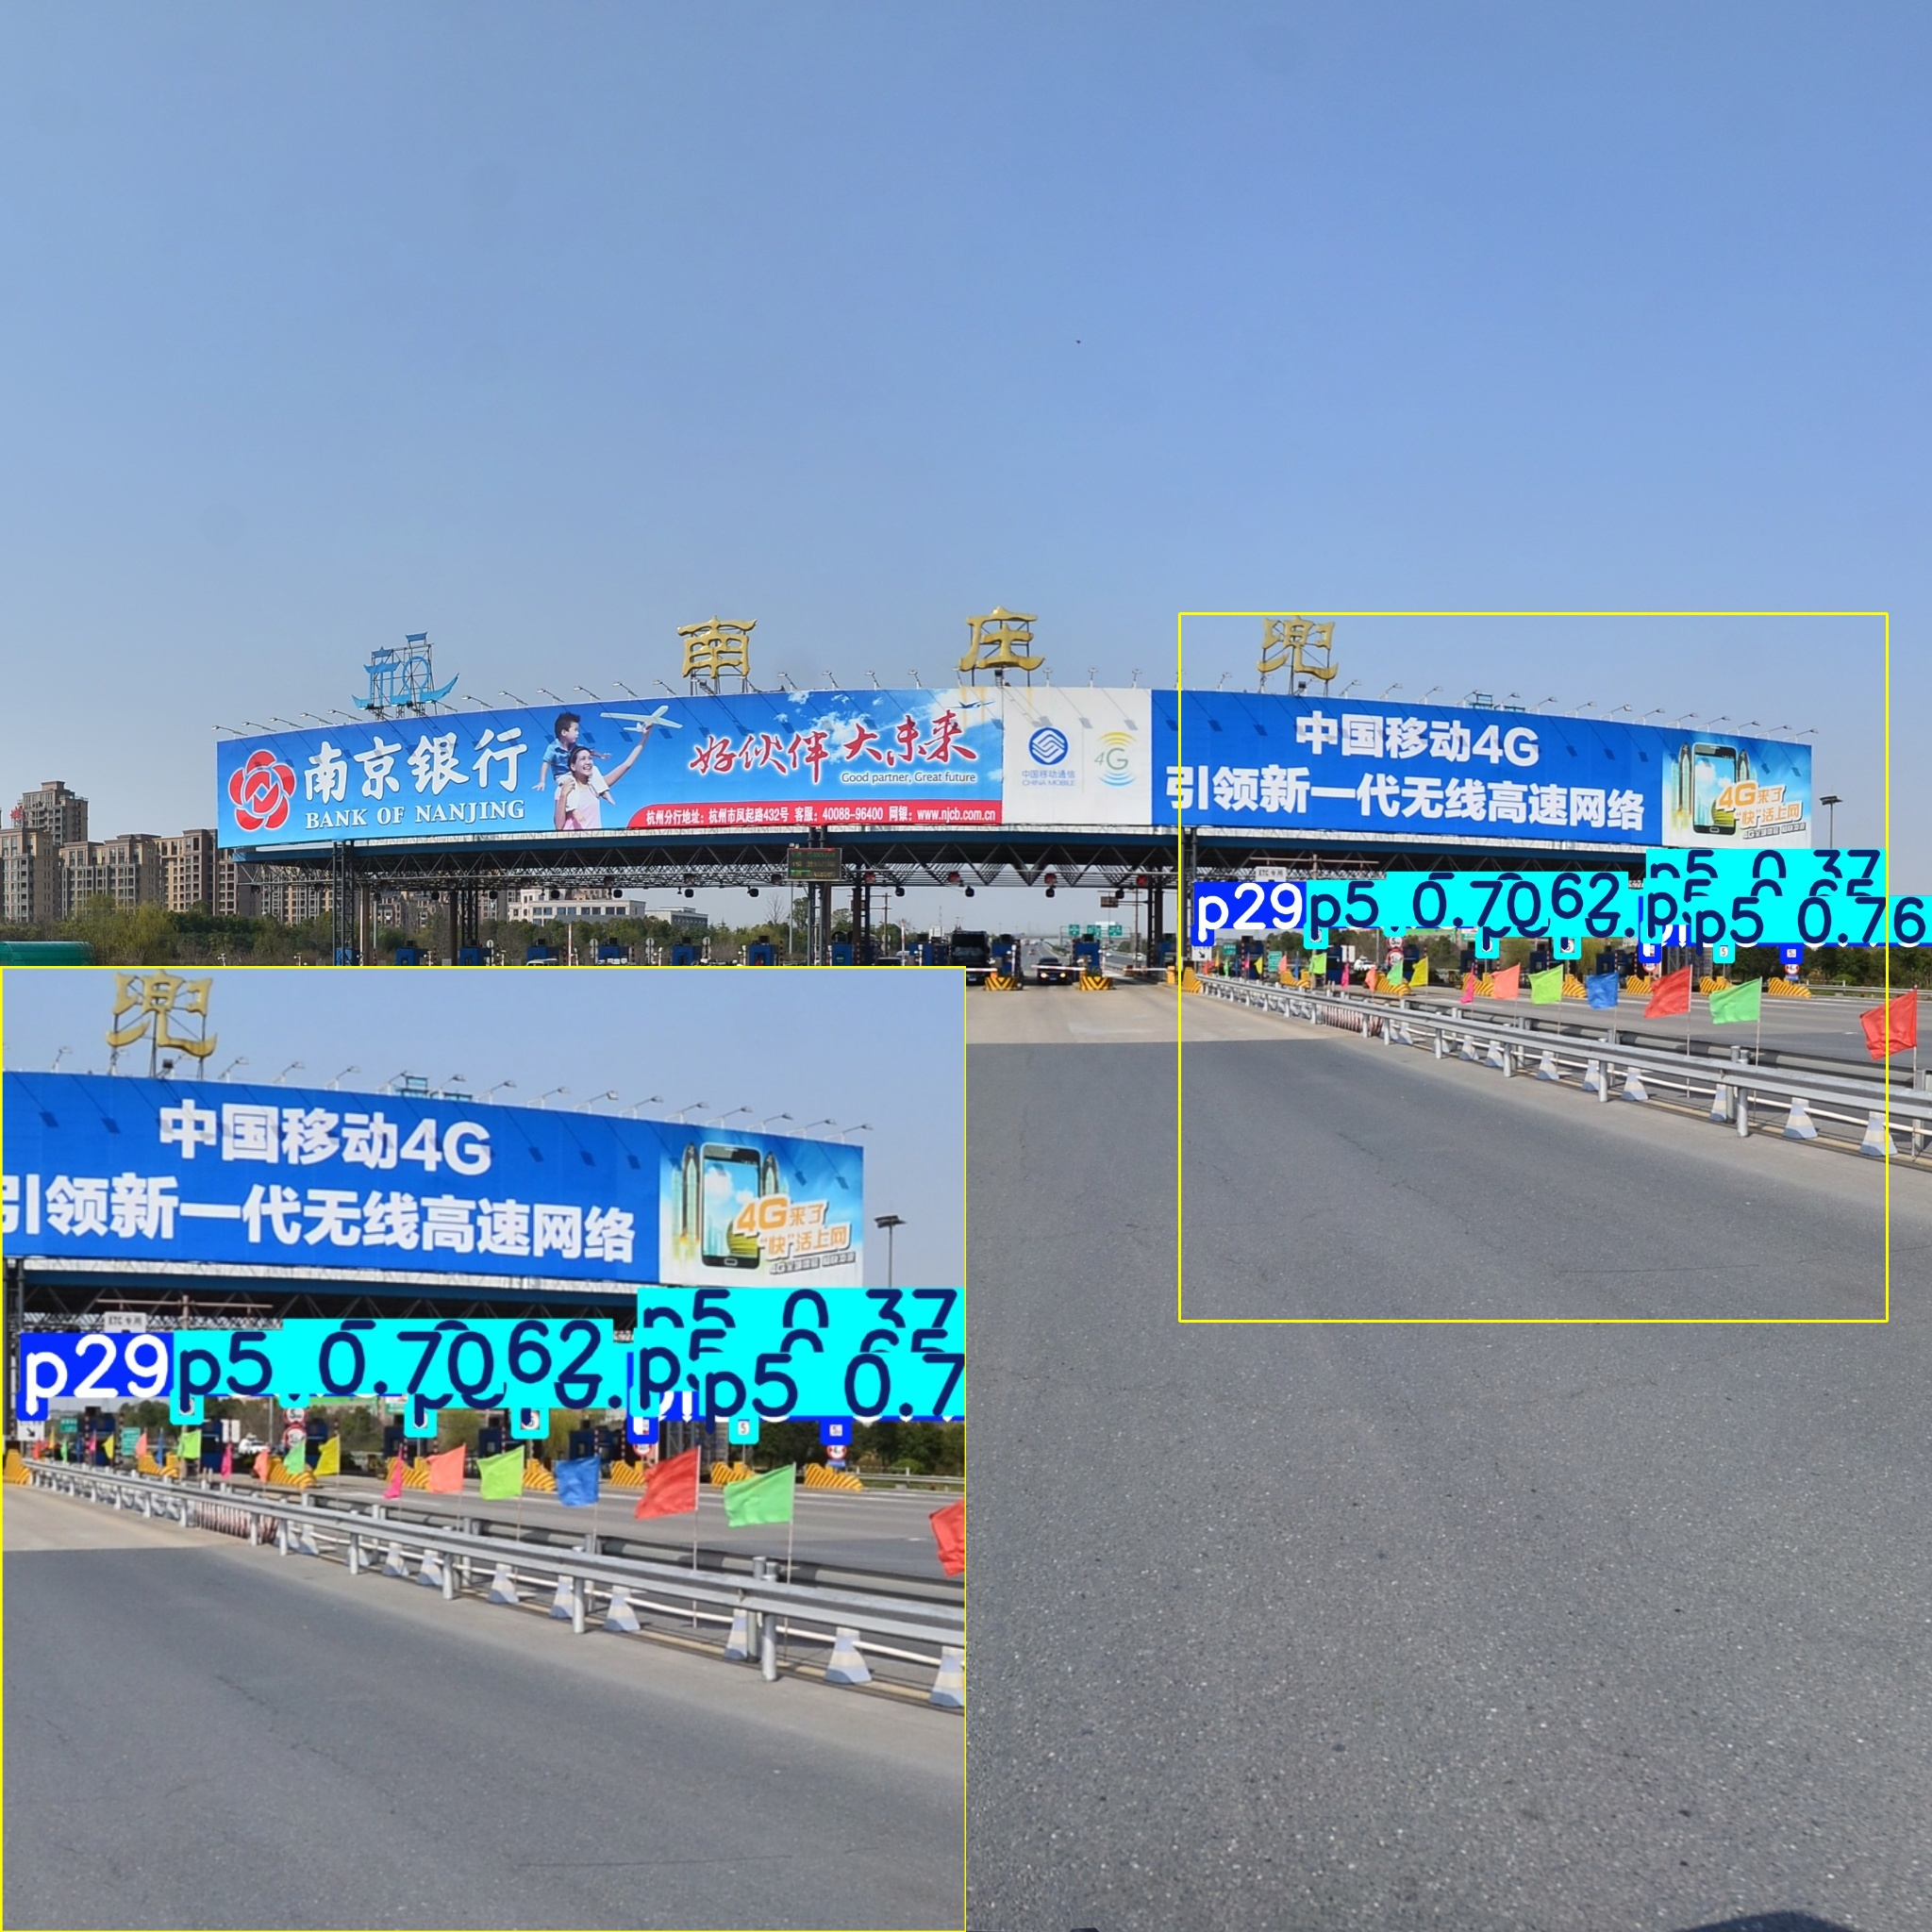
\includegraphics[width=0.45\textwidth]{../figure/ex-yolos_tt100k_44171.jpg}%
        } 
        \subfloat[YOLOv11s\label{fig:tt100k_1_11}]{%
            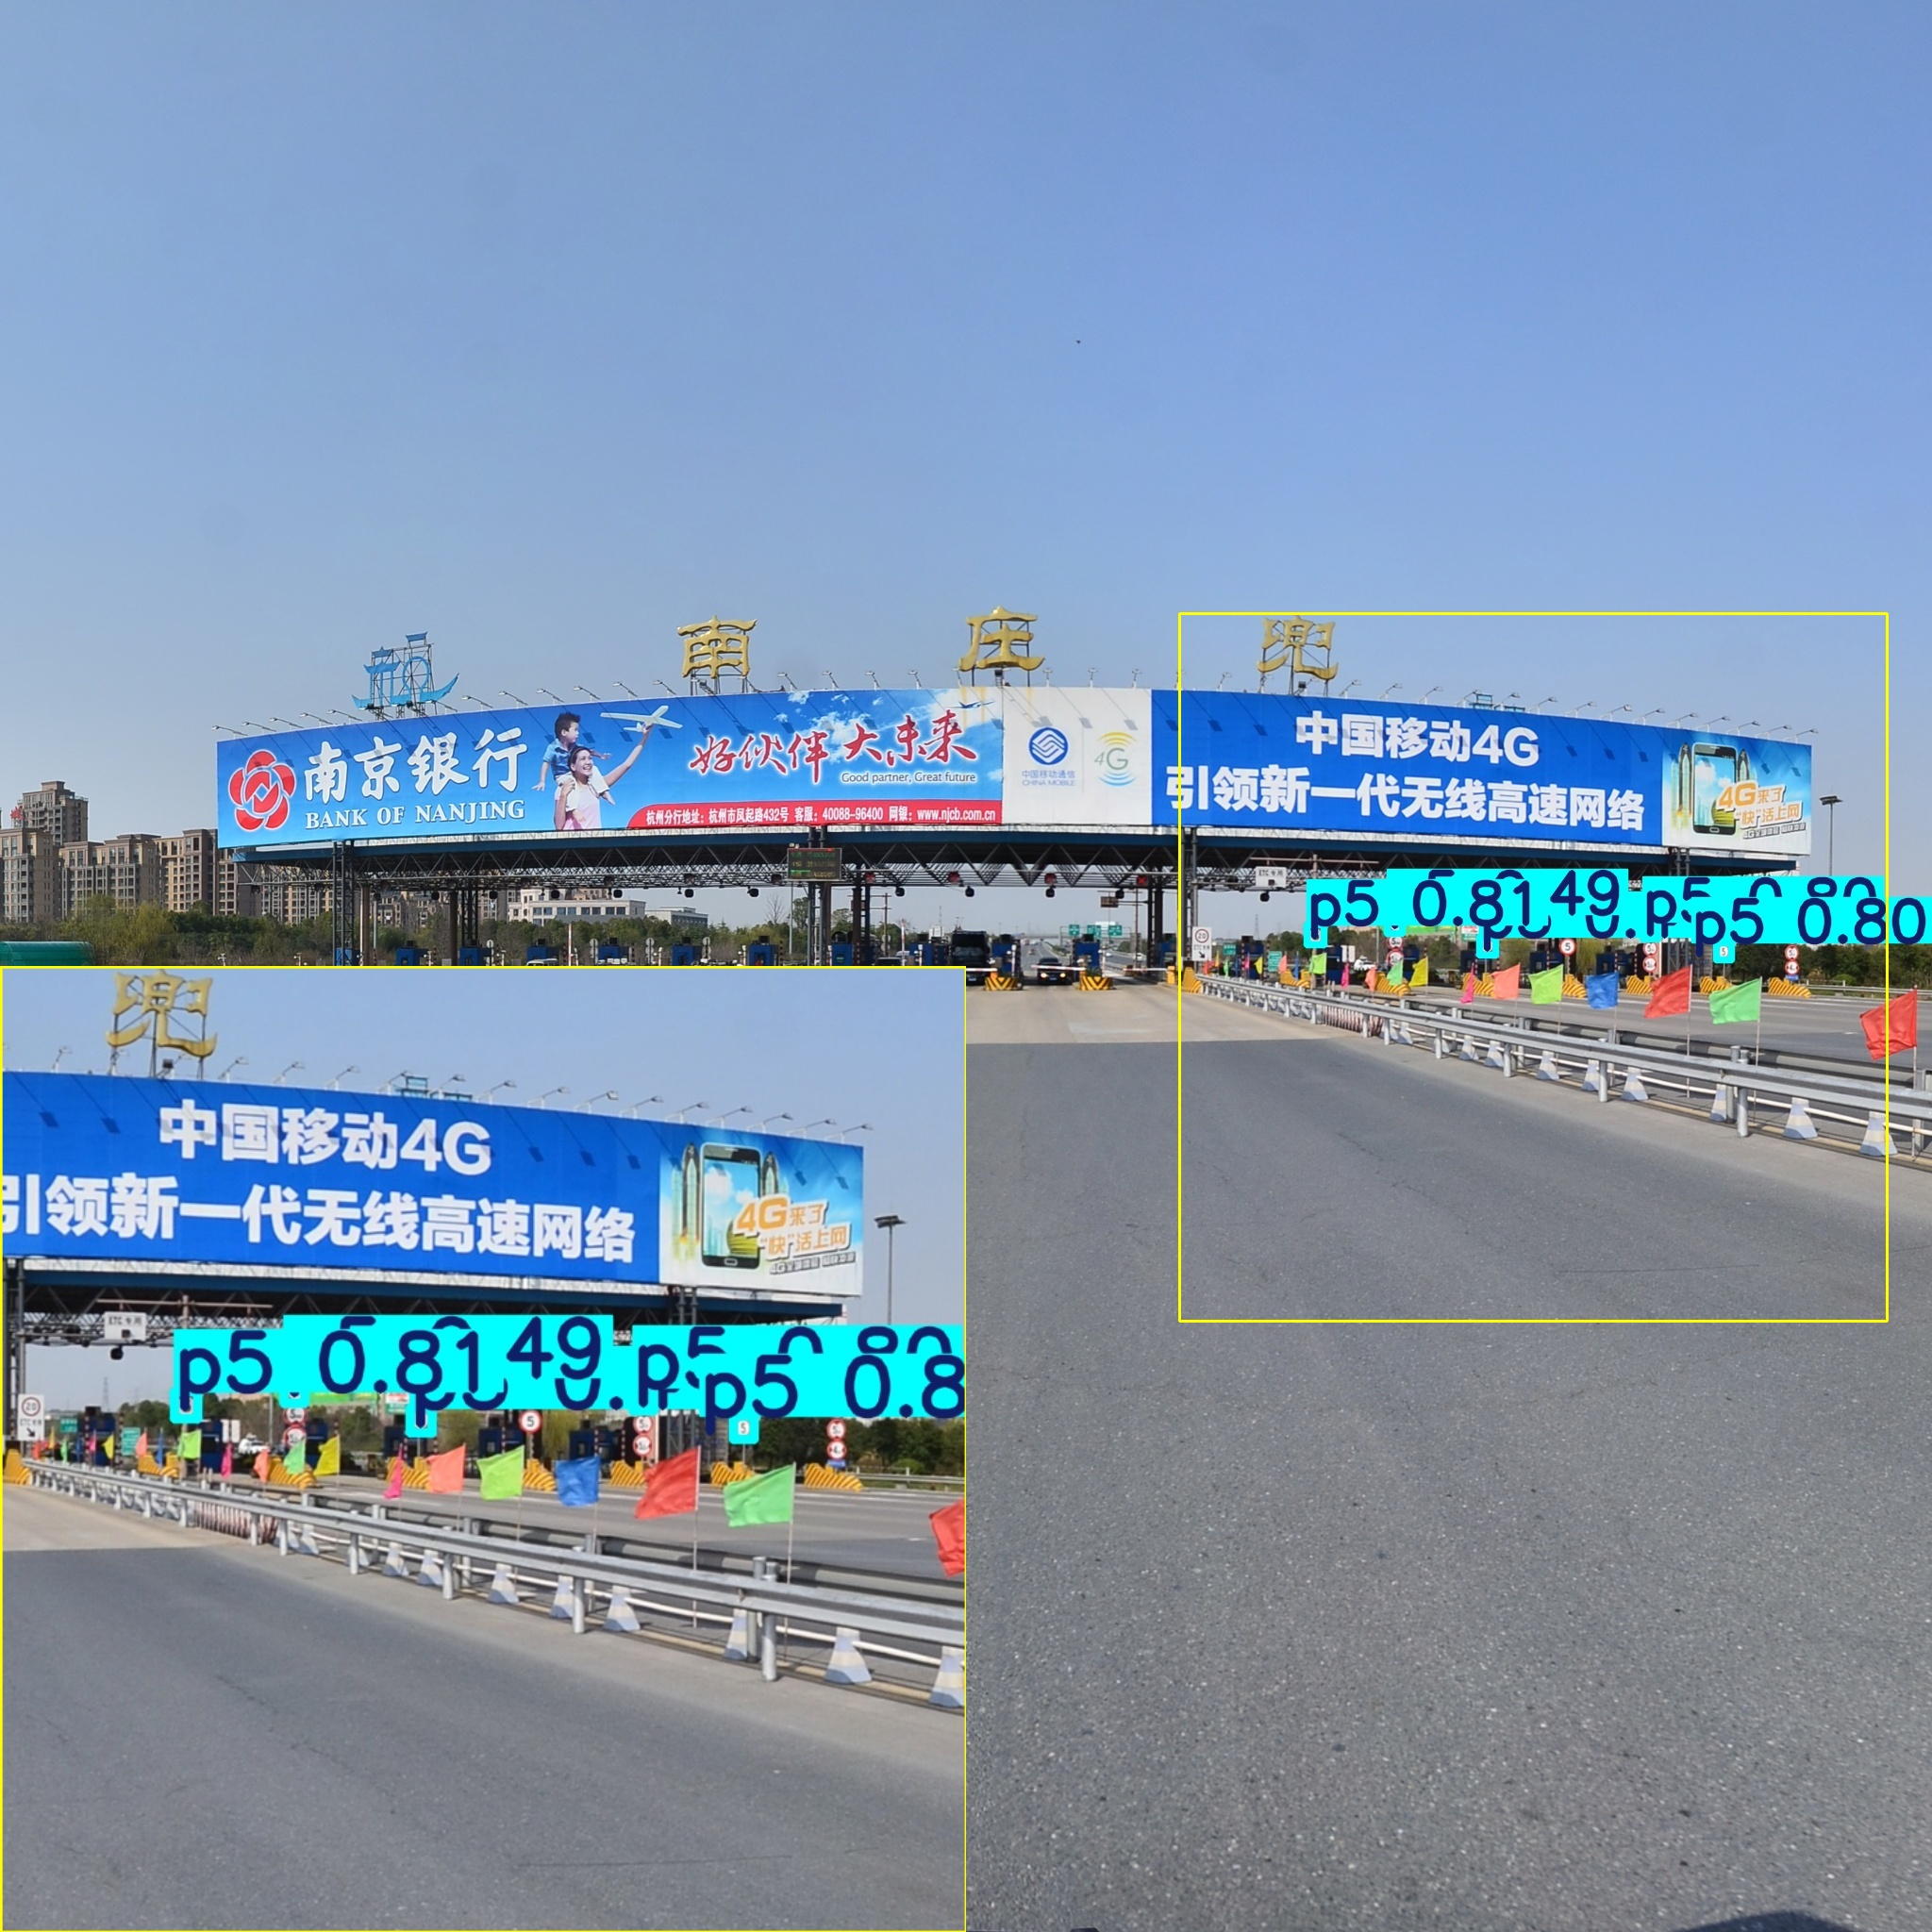
\includegraphics[width=0.45\textwidth]{../figure/v11s_tt100k_44171.jpg}%
        }
        \\
        \subfloat[YOLOv10s\label{fig:tt100k_1_10}]{%
            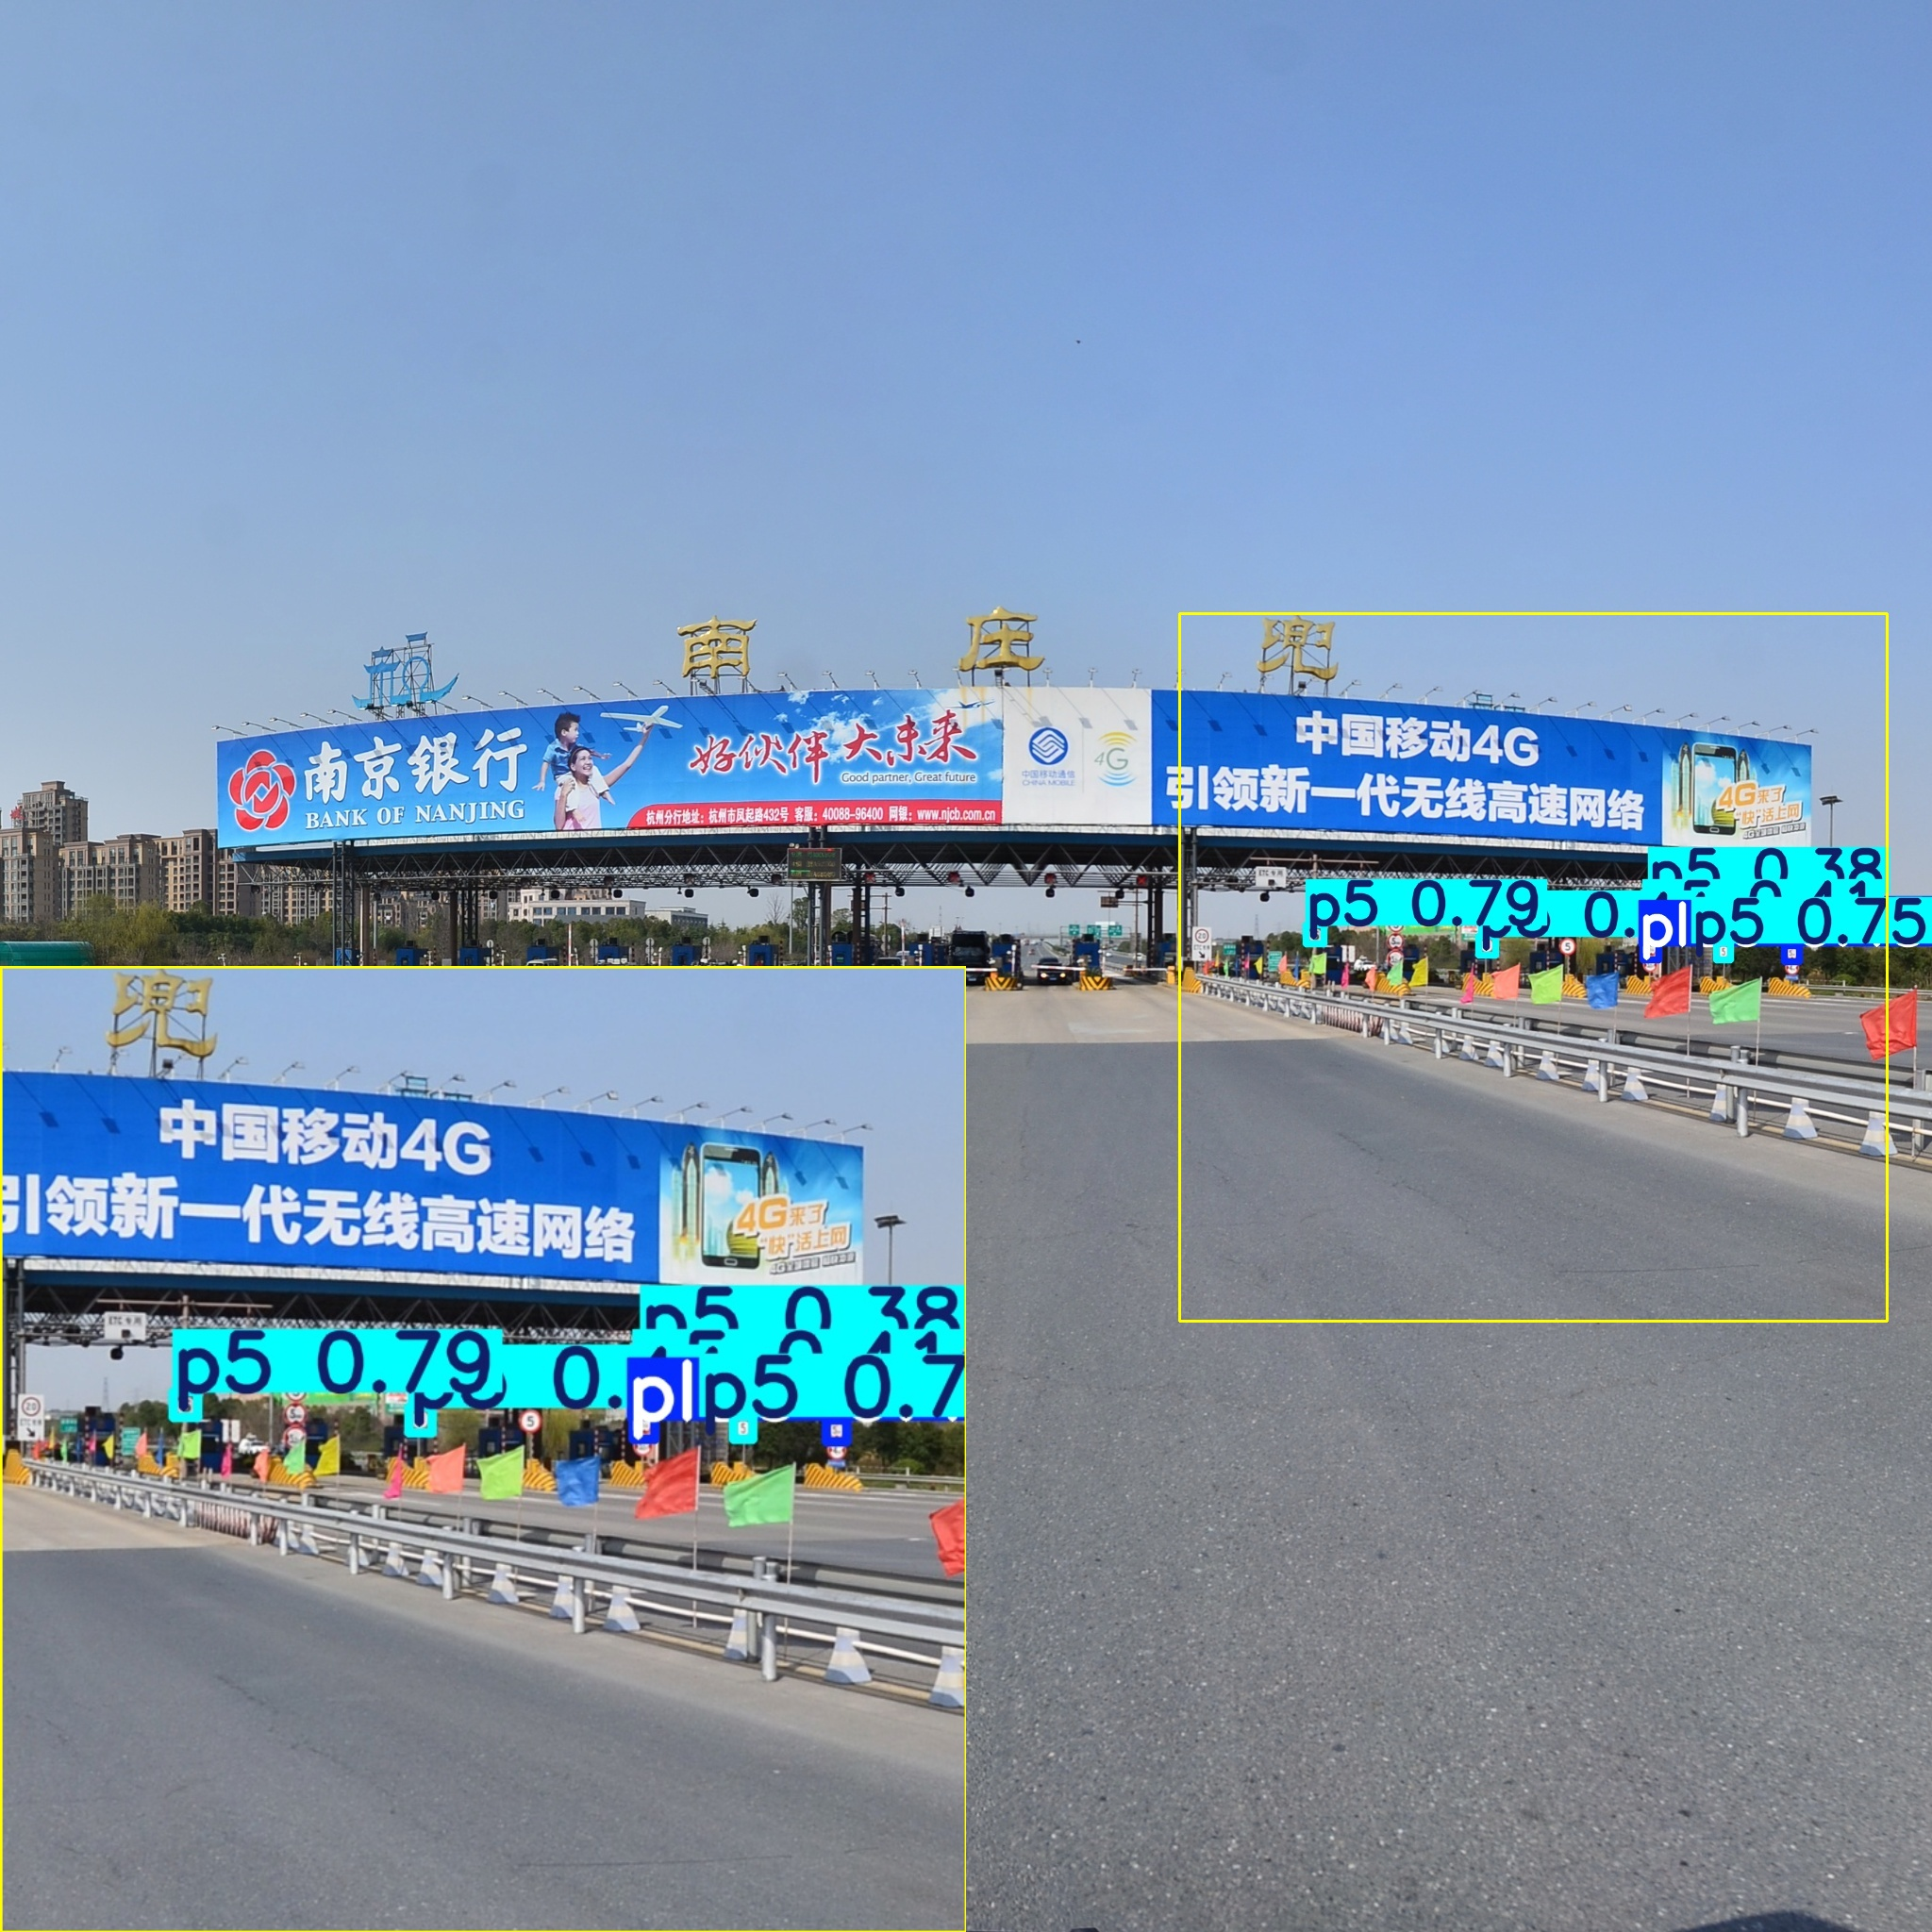
\includegraphics[width=0.45\textwidth]{../figure/v10s_tt100k_44171.jpg}%
        }
        \subfloat[YOLOv9s\label{fig:tt100k_1_9}]{%
            \includegraphics[width=0.45\textwidth]{../figure/v9s_tt100k_44171.jpg}%
        }
    \captionsetup{font=footnotesize}
    \bicaption{不同网络模型在TT100K数据集上的推理结果}{Some descriptions of the pictures in question.}
    \label{fig:tt100k_compare_1}
\end{figure}

% \begin{figure}[htbp]
%     \centering
%         \subfloat[EX-YOLO\label{fig:tt100k_2_ex}]{%
%             \includegraphics[width=0.33\textwidth]{../figure/ex-yolos_tt100k_44171.jpg}%
%         } 
%         \subfloat[YOLOv11s\label{fig:tt100k_2_11}]{%
%             \includegraphics[width=0.33\textwidth]{../figure/v11s_tt100k_44171.jpg}%
%         }
%         \\
%         \subfloat[YOLOv10s\label{fig:tt100k_2_10}]{%
%             \includegraphics[width=0.33\textwidth]{../figure/v10s_tt100k_44171.jpg}%
%         }
%         \subfloat[YOLOv9s\label{fig:tt100k_2_9}]{%
%             \includegraphics[width=0.33\textwidth]{../figure/v9s_tt100k_44171.jpg}%
%         }
%     \captionsetup{font=footnotesize}
%     \bicaption{不同网络模型在TT100K数据集上的推理结果}{Some descriptions of the pictures in question.}
%     \label{fig:tt100k_compare_2}
% \end{figure}

在图\ref{fig:tt100k_compare_1}
% 和图\ref{fig:tt100k_compare_2}
的比较实验中,选择了TT100K数据集中具有复杂场景和干扰的图像。
图\ref{fig:tt100k_compare_1}显示,由于目标场景的复杂性,YOLOv9s无法检测到图片中的所有目标信息,YOLOv10s只能检测到一小部分目标信息,而YOLOv11s和EX-YOLO检测到更完整的目标信息。 可以看出,YOLOv9和YOLOv10在检测小目标方面仍然存在一些问题。 相比之下,EX-YOLO可以用低计算能力准确检测正确的目标。
% 图\ref{fig:tt100k_compare_2}显示,由于目标场景的复杂性,YOLOv9s无法检测到图片中的所有目标信息,YOLOv10s只能检测到一小部分目标信息,而YOLOv11s和EX-YOLO检测到更完整的目标信息。 可以看出,YOLOv9和YOLOv10在检测小目标方面仍然存在一些问题。 相比之下,EX-YOLO可以用低计算能力准确检测正确的目标。

\begin{figure}[htbp]
    \centering
        \subfloat[EX-YOLO\label{fig:vd_1_ex}]{%
        \includegraphics[width=0.48\textwidth]{../figure/ex-YOLOs_VisDrone_0000151_00348_d_0000133.jpg}} 
        \subfloat[YOLOv11s\label{fig:vd_1_11}]{%
        \includegraphics[width=0.48\textwidth]{../figure/v11s_VisDrone_0000151_00348_d_0000133.jpg}}
        \\
        \subfloat[YOLOv10s\label{fig:vd_1_10}]{%
        \includegraphics[width=0.48\textwidth]{../figure/v10s_VisDrone_0000151_00348_d_0000133.jpg}}
        \subfloat[YOLOv9s\label{fig:vd_1_9}]{%
        \includegraphics[width=0.48\textwidth]{../figure/v9s_VisDrone_0000151_00348_d_0000133.jpg}}
    \captionsetup{font=footnotesize}
    \bicaption{不同网络模型在VisDrone数据集上的推理结果}{Some descriptions of the pictures in question.}
    \label{fig:vd_compare_1}
\end{figure}

% \begin{figure}[htbp]
%     \centering
%         \subfloat[EX-YOLO\label{fig:vd_2_ex}]{%
%         \includegraphics[width=0.4\textwidth]{../figure/ex-YOLOs_VisDrone_0000151_00348_d_0000133.jpg}} 
%         \subfloat[YOLOv11s\label{fig:vd_2_11}]{%
%         \includegraphics[width=0.4\textwidth]{../figure/v11s_VisDrone_0000151_00348_d_0000133.jpg}}
%         \\
%         \subfloat[YOLOv10s\label{fig:vd_2_10}]{%
%         \includegraphics[width=0.4\textwidth]{../figure/v10s_VisDrone_0000151_00348_d_0000133.jpg}}
%         \subfloat[YOLOv9s\label{fig:9}]{%
%         \includegraphics[width=0.4\textwidth]{../figure/v9s_VisDrone_0000151_00348_d_0000133.jpg}}
%     \captionsetup{font=footnotesize}
%     \bicaption{不同网络模型在VisDrone数据集上的推理结果}{Some descriptions of the pictures in question.}
%     \label{fig:vd_compare_2}
% \end{figure}

在图\ref{fig:vd_compare_1}
% 和图\ref{fig:vd_compare_2}
的比较实验中,在VisDrone数据集中选择具有复杂场景、小而密集的目标、各种目标、模糊和干扰的图像。
在图\ref{fig:vd_compare_1}中,所有模型的探测器都无法检测到所有检测目标,只能检测其中的一部分。 可以看出,YOLOv9s表现最好,这与其高mAP相吻合。 YOLOv10s和YOLOv11s在检测具有各种目标、模糊和干扰的小型密集目标方面仍然没有足够的性能。 相比之下,EX-YOLO可以在低计算量下准确检测更准确的目标,显示出接近YOLOv9s的检测性能,并且可以在复杂和重叠的场景中准确检测更多目标。 从图\ref{fig:vd_compare_1}可以看出,EX-YOLO的检测性能明显优于YOLOv10s和YOLOv11s,但略低于YOLOv9s。
% 在图\ref{fig:vd_compare_2}中,所有模型的探测器都无法检测到所有检测目标,只能检测其中的一部分。 可以看出,YOLOv9s表现最好,这与其高mAP相吻合。 YOLOv10s和YOLOv11s在检测具有各种目标、模糊和干扰的小型密集目标方面仍然没有足够的性能。 相比之下,EX-YOLO可以在低计算量下准确检测更准确的目标,显示出接近YOLOv9s的检测性能,并且可以在复杂和重叠的场景中准确检测更多目标。 从图\ref{fig:vd_compare_2}可以看出,EX-YOLO的检测性能明显优于YOLOv10s和YOLOv11s,但略低于YOLOv9s。

根据图\ref{fig:tt100k_compare_1}、
% 图\ref{fig:tt100k_compare_2}、
图\ref{fig:vd_compare_1}
% 和图\ref{fig:vd_compare_2}
,当目标分布不均匀且分布不密集时,YOLOv11s可以实现更好的识别性能,而YOLOv9s可以在目标分布密集的条件下正确捕获更多目标。 EX-YOLO可以平衡这两种情况,以实现尽可能高的识别性能,这显然优于YOLOv10s,EX-YOLO大大减少了计算量。 这有利于无人机在面对复杂场景时识别小目标。

\subsection{本章小结}

本研究聚焦交通小目标检测难题,对 YOLOv11 网络进行深度改进,提出 EX-YOLO 算法。YOLOv11 以改进的 CSPDarknet 为骨干网络,其多层特征金字塔与 CSP 模块设计在特征提取的深度与广度上达成平衡,为复杂场景目标检测奠定基础。特征融合网络借助 FPN 和 PANet 实现多尺度特征融合与自适应加权,提升检测精度与鲁棒性。但传统 YOLO 框架在交通小目标检测中存在浅层特征图分辨率不足、跨尺度融合效率低及背景噪声干扰分类置信度等问题。

针对上述挑战,本研究提出创新改进措施。改进的特征融合模块 SPPC 融合 SPPF 的多尺度特征提取与 CAM 的特征增强能力,显著提升小目标特征捕获能力,提高 mAP。轻量化卷积模块 DBSS 结合深度可分离卷积(DSC)与 SimAM 注意力模块,在降低计算复杂度的同时保持高精度,减少模型参数量与计算量,适用于资源受限设备。引入的 NWD 损失函数与 DIoU 损失函数结合,精准计算预测框与真实框的空间和规模差异,增强小目标检测能力,尤其在小目标定位精度方面表现出色。

实验在 TT100K 和 VisDrone 数据集上验证 EX-YOLO 算法。结果显示,EX-YOLO 在参数量、计算量、精度、召回率和 FPS 等关键指标上综合性能优异。与 YOLOv11s、YOLOv10s 和 YOLOv9s 等基准模型相比,EX-YOLO 在保持较高检测精度的同时大幅降低计算量,平衡精度与效率。例如,在 TT100K 数据集上,EX-YOLO 的 mAP0.5 为 0.893,略低于 YOLOv9s 的 0.906,但计算量仅为其 62.5\%(17.0 GFLOPs 对比 27.2 GFLOPs)。在 VisDrone 数据集上,EX-YOLO 的 mAP0.5 与 YOLOv10s 相同(0.390),计算量却仅为后者的 62.8\%(15.4 GFLOPs 对比 24.5 GFLOPs)。消融实验进一步证实各改进模块的有效性,NWD 损失函数、SPPC 模块和 DBSS 模块在提升检测性能与优化计算效率方面发挥关键作用。

实验表明,EX-YOLO 算法在交通小目标检测领域竞争优势显著,尤其适用于资源受限场景。通过引入创新模块,本研究增强 YOLOv11 模型的小目标检测实用性,降低计算资源需求,使其更适配无人机等有限设备环境。未来,随着深度学习技术发展,EX-YOLO 算法有望在智能交通系统、无人机监控等领域发挥更大作用,助力高效精准的交通目标检测。
\newpage

\section{方法B\label{方法B}}

\begin{figure}[htb]
    \centering
    \subfloat{
        \includegraphics[width=0.45\linewidth]{P1.jpg}
    }%\hfill
    \subfloat{
        \includegraphics[width=0.45\linewidth]{P2.jpg}
    }\\
    \captionsetup{font=footnotesize}
    \bicaption{一些有关图片的描述。}{Some descriptions of the pictures in question.}
    \label{fig:幂律参数空间B}
\end{figure}

\subsection{方法B的二级标题}

方法B二级标题的正文,方法B二级标题的正文,方法B二级标题的正文,方法B二级标题的正文,方法B二级标题的正文。

\subsubsection{方法B的三级标题}

方法B三级标题的正文,方法B三级标题的正文,方法B三级标题的正文,方法B三级标题的正文,方法B三级标题的正文。


% Please add the following required packages to your document preamble:
% \usepackage{booktabs}
\begin{table}[htb]
    \centering
    \captionsetup{font=footnotesize}
    \bicaption{符号对照表}{Symbol cross-reference table}
    \label{tab:符号对照表B}
    \begin{tabular}{@{}cc@{}}
        \toprule
        符号     & 含义       \\ 
        \midrule
        $a$     & 尺度因子    \\
        $k$     & 波尔兹曼常数 \\
        $T_c$   & 一些描述    \\
        $\beta$ & 一些描述    \\
        $t_b$   & 一些描述    \\
        \bottomrule
    \end{tabular}
\end{table}

\subsection{方法B的二级标题}

方法B二级标题的正文,方法B二级标题的正文,方法B二级标题的正文,方法B二级标题的正文,方法B二级标题的正文。

\subsubsection{方法B的三级标题}

方法B三级标题的正文,方法B三级标题的正文,方法B三级标题的正文,方法B三级标题的正文,方法B三级标题的正文。
\newpage

\section{雾天交通目标检测结果分析\label{实验结果分析}}

\subsection{雾天交通目标检测流程}

实验结果分析二级标题的正文,实验结果分析二级标题的正文,实验结果分析二级标题的正文,实验结果分析二级标题的正文,实验结果分析二级标题的正文。

\subsection{DH-YOLO网络分析}

实验结果分析三级标题的正文,实验结果分析三级标题的正文,实验结果分析三级标题的正文,实验结果分析三级标题的正文,实验结果分析三级标题的正文。

\subsection{实验结果和分析}


\subsection{本章小结}


\newpage

\section{结论\label{结论}}

\subsection{总结}

结论二级标题的正文,结论二级标题的正文,结论二级标题的正文,结论二级标题的正文,结论二级标题的正文。

\subsection{展望}

结论三级标题的正文,结论三级标题的正文,结论三级标题的正文,结论三级标题的正文,结论三级标题的正文。
\newpage

\pagebreak
{\zihao{5}\bibliography{references}}
\pagebreak

% \begin{appendices}
% \appendix
\setcounter{table}{0}
\setcounter{figure}{0}
\setcounter{equation}{0}
\renewcommand{\thetable}{\thesection-\arabic{table}}
\renewcommand{\theequation}{\thesection-\arabic{equation}}
\renewcommand{\thefigure}{\thesection-\arabic{figure}}

\ctexset{section={name={附录},number=\thesection}}%修改章节序号以符合附录
    
\section{第一个附录\label{附录:第一个附录}}
周后稷,名弃。其母有邰氏女,曰姜原。姜原为帝喾元妃。姜原出野,见巨人迹,心忻然说,欲践之,践之而身动如孕者。居期而生子,以为不祥,弃之隘巷,马牛过者皆辟不践;徙置之林中,適会山林多人,迁之;而弃渠中冰上,飞鸟以其翼覆荐之。姜原以为神,遂收养长之。初欲弃之,因名曰弃。

弃为兒时,屹如巨人之志。其游戏,好种树麻、菽,麻、菽美。及为成人,遂好耕农,相地之宜,宜穀者稼穑焉,民皆法则之。帝尧闻之,举弃为农师,天下得其利,有功。帝舜曰:“弃,黎民始饥,尔后稷播时百穀。”封弃於邰,号曰后稷,别姓姬氏。后稷之兴,在陶唐、虞、夏之际,皆有令德。

\pagebreak %强制结束此页,也可以使用\newpage代替


\section{第二个附录\label{附录:第二个附录}}
崇侯虎谮西伯於殷纣曰:“西伯积善累德,诸侯皆向之,将不利於帝。”帝纣乃囚西伯於羑里。闳夭之徒患之。乃求有莘氏美女,骊戎之文马,有熊九驷,他奇怪物,因殷嬖臣费仲而献之纣。纣大说,曰:“此一物足以释西伯,况其多乎!”乃赦西伯,赐之弓矢斧钺,使西伯得征伐。曰:“谮西伯者,崇侯虎也。”西伯乃献洛西之地,以请纣去砲格之刑。纣许之。

西伯阴行善,诸侯皆来决平。於是虞、芮之人有狱不能决,乃如周。入界,耕者皆让畔,民俗皆让长。虞、芮之人未见西伯,皆惭,相谓曰:“吾所争,周人所耻,何往为,祇取辱耳。”遂还,俱让而去。诸侯闻之,曰“西伯盖受命之君”。

\end{appendices}

% \pagebreak

\section*{攻读学位期间发表论文与研究成果清单}\addcontentsline{toc}{section}{攻读学位期间发表论文与研究成果清单}

% \noindent[1]\ Wang X Z, Deng C M. The primordial black holes solution to the cosmological monopole problem[J]. The European Physical Journal C, 2024, 84(1): 31.

发表论文:
1. 《Springer LNCS》期刊的1篇 CCF-C 会议论文,第一作者(已录用待刊)。
\pagebreak

\end{document}
